%%%%%%%%%%%%%%%%%%%%%%%%%%%%%%%%%%%
%%%%%%%%%%%%%%%%%%%%%%%%%%%%%%%%%%%
%%% if Kindle %%%%%%%%%%%%%%%%%%%%%
%\documentclass[6pt]{scrreprt}
%\usepackage[papersize={4.8in,3.5in},margin=2mm]{geometry}
%\usepackage[frame,center]{crop}
%%%%%%%%%%%%%%%%%%%%%%%%%%%%%%%%%%%
%%% if DinA4 %%%%%%%%%%%%%%%%%%%%%%
\documentclass[a4paper]{scrreprt}
\usepackage[left=2cm,right=2cm,top=2.5cm,bottom=2.5cm]{geometry}
%%%%%%%%%%%%%%%%%%%%%%%%%%%%%%%%%%%
%%%%%%%%%%%%%%%%%%%%%%%%%%%%%%%%%%%

% Usepackages, Kurzbefehle, etc.
\usepackage[ngerman]{babel}
\usepackage[utf8]{inputenc}

% Klickbare Verknüpfungen
\usepackage[hidelinks]{hyperref}

% Hübsche Header
\usepackage{fancyhdr}
\pagestyle{fancy}

% Zusätzliche Symbole (u.a. Widerspruchsblitz)
\usepackage{marvosym}

% Grafiken importieren
\usepackage{graphicx}

% Farben
\usepackage{xcolor}

% Zeichenpaket (Graphen, Zahlenstrahl, etc.)
\usepackage{tikz}
\usetikzlibrary{decorations.pathreplacing}
\usetikzlibrary{lindenmayersystems}
\usetikzlibrary{patterns}
\newcommand{\streiche}[1]{%
    \tikz[baseline=(tocancel.base)]{
        \node[inner sep=0pt,outer sep=0pt] (tocancel) {#1};
        \draw[red] (tocancel.south west) -- (tocancel.north east);
    }%
}%

\newlength{\hatchspread}
\newlength{\hatchthickness}
\newlength{\hatchshift}
\newcommand{\hatchcolor}{}
% declaring the keys in tikz
\tikzset{hatchspread/.code={\setlength{\hatchspread}{#1}},
         hatchthickness/.code={\setlength{\hatchthickness}{#1}},
         hatchshift/.code={\setlength{\hatchshift}{#1}},% must be >= 0
         hatchcolor/.code={\renewcommand{\hatchcolor}{#1}}}
% setting the default values
\tikzset{hatchspread=3pt,
         hatchthickness=0.4pt,
         hatchshift=0pt,% must be >= 0
         hatchcolor=black}
% declaring the pattern
\pgfdeclarepatternformonly[\hatchspread,\hatchthickness,\hatchshift,\hatchcolor]% variables
   {custom north west lines}% name
   {\pgfqpoint{\dimexpr-2\hatchthickness}{\dimexpr-2\hatchthickness}}% lower left corner
   {\pgfqpoint{\dimexpr\hatchspread+2\hatchthickness}{\dimexpr\hatchspread+2\hatchthickness}}% upper right corner
   {\pgfqpoint{\dimexpr\hatchspread}{\dimexpr\hatchspread}}% tile size
   {% shape description
    \pgfsetlinewidth{\hatchthickness}
    \pgfpathmoveto{\pgfqpoint{0pt}{\dimexpr\hatchspread+\hatchshift}}
    \pgfpathlineto{\pgfqpoint{\dimexpr\hatchspread+0.15pt+\hatchshift}{-0.15pt}}
    \ifdim \hatchshift > 0pt
      \pgfpathmoveto{\pgfqpoint{0pt}{\hatchshift}}
      \pgfpathlineto{\pgfqpoint{\dimexpr0.15pt+\hatchshift}{-0.15pt}}
    \fi
    \pgfsetstrokecolor{\hatchcolor}
%    \pgfsetdash{{1pt}{1pt}}{0pt}% dashing cannot work correctly in all situation this way
    \pgfusepath{stroke}
   }


% Linie unten
\renewcommand{\footrulewidth}{0.5pt}
% Kopfzeile Linie oben
\renewcommand{\headrulewidth}{0.5pt}
% Fußzeile
\fancyfoot[C]{- \thepage\ -}
% Kopfzeilen fürs Inhaltsverzeichnis:
% Kopfzeile links bzw. innen
\fancyhead[L]{\Large Inhaltsverzeichnis}
% Kopfzeile rechts bzw. außen
\fancyhead[R]{\Large{}}
% Kopfzeile beim Kapitelanfang:
\fancypagestyle{plain}{
	% Kopfzeilen fürs Inhaltsverzeichnis:
	% Kopfzeile links bzw. innen
	\fancyhead[L]{\Large Inhaltsverzeichnis}
	% Kopfzeile rechts bzw. außen
	\fancyhead[R]{\Large{}}
}

\usepackage{tocloft}
\renewcommand\cftsecnumwidth{1.2cm}
\renewcommand\cftchapnumwidth{0.75cm}

\setcounter{chapter}{-1} %Überschriftennummer neu setzen (zahl der bereits vergebenen Nummern)
\renewcommand{\thechapter}{§\arabic{chapter}}
\renewcommand{\thesection}{\arabic{chapter}.\arabic{section}}
\setcounter{tocdepth}{2}


% Mathegedöns
\usepackage{amsmath}%Mathebiblothek
\usepackage{amssymb} %Sonderzeichen (z.B. \checkmark)
\usepackage{enumitem}%Aufzählunden formatieren
\usepackage{polynom}

% Kurzbefehle

%Zahlenmengen start
\newcommand{\C}{\mathbb{C}}%komplexe Zahlen
\newcommand{\R}{\mathbb{R}}%reelle Zahlen
\newcommand{\Q}{\mathbb{Q}}%rationale Zahlen
\newcommand{\Z}{\mathbb{Z}}%ganze Zahlen
\newcommand{\N}{\mathbb{N}}%Natürliche Zahlen
\newcommand{\Lsg}{\mathbb{L}}%Lösungsmenge 
\newcommand{\F}{\mathbb{F}}%Körper (z.B. F_2)
\newcommand{\K}{\mathbb{K}}%Körper (z.B. K_2)
%Zahlenmengen end

\newcommand{\A}{\mathcal{A}} % Geschwungenes A
\newcommand{\E}{\mathcal{E}} % Geschwungenes E/großes Epsilon
\newcommand{\Pow}{\mathcal{P}} % Potenzmenge (engl. Power Set)
\newcommand{\eps}{\varepsilon}
\newcommand{\ok}{\hfill{\checkmark}}
\newcommand{\qed}{\hfill{q.e.d.}}
\newcommand{\wspruch}{\Lightning}
\newcommand{\nl}{\\[8pt]} %für Absätze
\newcommand{\es}{\emptyset}
\newcommand{\rem}[1]{} %Blockweise kommentieren ;)
%Aufzählung Zahlen
\newcommand{\en}[1]{\begin{enumerate}[label=(\arabic*)] #1 \end{enumerate}}
%Aufzählung Zahlen (ohne Klammer, mit Punkt)
\newcommand{\enk}[1]{\begin{enumerate}[label=\arabic*.] #1 \end{enumerate}}
%Aufzählung Buchstaben
\newcommand{\ena}[1]{\begin{enumerate}[label=(\alph*)] #1 \end{enumerate}}
%Aufzählung Römische Buchstaben
\newcommand{\enr}[1]{\begin{enumerate}[label=(\roman*)] #1 \end{enumerate}}
%Aufzählung Römische Großbuchstaben
\newcommand{\enR}[1]{\begin{enumerate}[label=(\Roman*)] #1 \end{enumerate}}
%Aufzählung
\newcommand{\items}[1]{\begin{itemize} #1 \end{itemize}}

% Große Summe, Produkt, Binomialkoeffizient, ...
\newcommand{\bigsum}{\displaystyle\sum}
\newcommand{\bigprod}{\displaystyle\prod}
\newcommand{\bigbin}{\displaystyle\binom}
\newcommand{\biglim}{\displaystyle\lim}
\newcommand{\bigfrac}{\displaystyle\frac}

% Große Klammern
\newcommand{\bigbrackets}[1]{\left( #1 \right)}
\newcommand{\bigbraces}[1]{\left\{ #1 \right\}}
% Auskommentieren, um große Schreibweise zu forcieren
\everymath{\displaystyle}

% "Nach Induktionsvoraussetzung" Gleich
\newcommand{\iv}{\underset{I.V.}{=}}

% Pfeile
\newcommand{\Ra}{\Rightarrow}
\newcommand{\La}{\Leftarrow}
\newcommand{\Lra}{\Leftrightarrow}
\newcommand{\rsa}{\rightsquigarrow}
\newcommand{\mto}{\mapsto}

% Grad von ... (Polynome)
\newcommand{\grad}{\text{grad }}

% Realteil, Imaginärteil
\newcommand{\RE}{\text{Re }}
\newcommand{\IM}{\text{Im }}

% Beginn Definition Dokument
\begin{document}
\title{Vorlesungsmitschrift\\Analysis für Informatiker}
\author{Michael Koch (Universität Paderborn)\\\texttt{\href{mailto:m.koch@emkay443.de}{m.koch@emkay443.de}}}
\date{Wintersemester 2013/14\\Stand: \today}
\maketitle

% Unterschiedliche Nummerierung IV/Inhalt
% Vielen Dank an Stefan Löwen für den Tipp. :)
\pagenumbering{Roman}
\tableofcontents\newpage
%% Kopfzeile beim Kapitelanfang:
\fancypagestyle{plain}{
%Kopfzeile links bzw. innen
\fancyhead[L]{}
%Kopfzeile rechts bzw. außen
\fancyhead[R]{}}
%Kopfzeile links bzw. innen
\fancyhead[L]{}
%Kopfzeile rechts bzw. außen
\fancyhead[R]{}
% **************************************************
\begin{center}
{\huge Frohe \href{http://www.stallman.org/grav-mass.html}{Schwernachten}!}\\
{\footnotesize\emph{(Feier von \href{https://de.wikipedia.org/wiki/Isaac_Newton}{Sir Isaac Newton}s Geburtstag, der nach dem \href{https://de.wikipedia.org/wiki/Julianischer_Kalender}{julianischen Kalender} auf den 25. Dezember fällt)}}\nl
\begin{tikzpicture}
\draw [color=green!50!black, l-system={rule set={S -> [+++G][---G]TS,
  G -> +H[-G]L, H -> -G[+H]L, T -> TL, L -> [-FFF][+FFF]F}, step=4pt, angle=18,
 axiom=+++++SLFFF, order=11}] lindenmayer system -- cycle;
\end{tikzpicture}\\
{\footnotesize\emph{Abbildung 1: Ein \href{https://de.wikipedia.org/wiki/Lindenmayer-System}{Lindenmayer-Schwernachtsbaum}}}\\[5mm]
\textbf{WE THREE LAWS OF ORBITING ARE}\nl
We three laws of orbiting are -\\
Ruling trajectories local and far -\\
Collisions billiard,\\
Particles myriad,\\
Planet and moon and star.\\
O-o-o-h ...\nl

Laws of wonder, laws of might,\\
Laws that steer the worlds aright,\\
Never failing - we are hailing\\
Your pow'r and mystery tonight!\nl

First Law am I, by Newton drawn:\\
An object in motion keeps moving on -\\
Ever proceeding, not slowing or speeding\\
Till another force acts thereon. O-o-o-h ...\nl

The Second Law, I come to say:\\
F is equal to m times a -\\
For acceleration calculation,\\
Second Law shows the way. O-o-o-h ...\nl

Third Law: to every action must be\\
An equal, opposing reaction. We\\
Now have said it - to Newton give credit,\\
Who gave us the Laws all three. O-o-o-h ...\nl

Laws of wonder, laws of might,\\
Laws that steer the worlds aright,\\
Never failing - we are hailing\\
Your pow'r and mystery tonight!\nl
{\footnotesize\emph{(Quelle: \href{http://www.stallman.org/we-three-laws.html}{http://www.stallman.org/we-three-laws.html})}}
\end{center}\newpage

%$\int\frac{x^{3}}{\sqrt{1+x^{2}}}dx=\int x^{3}\cdot\frac{1}{\sqrt{1+x^{2}}}dx$\\
$ \int \underbrace{x^{3}}_{u'}\cdot\underbrace{\frac{1}{\sqrt{1+x^{2}}}}_{v}dx= $
\newpage
% Kopfzeile beim Kapitelanfang:
\fancypagestyle{plain}{
%Kopfzeile links bzw. innen
\fancyhead[L]{\Large Wintersemester 2014/15}
%Kopfzeile rechts bzw. außen
\fancyhead[R]{}}
%Kopfzeile links bzw. innen
\fancyhead[L]{\Large Wintersemester 2014/15}
%Kopfzeile rechts bzw. außen
\fancyhead[R]{}
% **************************************************
\phantomsection
\addcontentsline{toc}{chapter}{Inhaltsverzeichnis für das Wintersemester 2014/15}
\chapter*{Inhaltsverzeichnis für das Wintersemester 2014/15}
Dieses Inhaltsverzeichnis erhebt keinen Anspruch auf Vollständigkeit!\\
Bitte besuchen Sie trotzdem die Vorlesung und Übungen, machen Sie die Heimübungen\\
und arbeiten Sie mit dem Buch \href{http://www.amazon.de/Analysis-Differential--Integralrechnung-Ver\%C3\%A4nderlichen-Mathematik/dp/3658003162/ref=sr\_1\_1?ie=UTF8\&qid=1414666359\&sr=8-1\&keywords=analysis+1+forster}{\textit{"`Analysis 1"' von Forster}}.
\section*{Einführung, Vorlesungsüberblick:}
\subsection*{2014-10-13 (Mo)}
\items{
\item Zahlenmystik: \href{http://de.wikipedia.org/wiki/Zahlensymbolik}{\textit{\underline{Wikipedia}}}
\item Assoziativ-, Kommutativ-, Distibutivgesetze: \ref{3.2}
\item Mengenlehre: \ref{Mengen}
\item Fibonacci: \ref{Fibonacci}
}

\subsection*{2014-10-16 (Do)}
\items{
\item Aussagen: \ref{Aussagen}
\item Mengenlehre: \ref{Mengen}
\item Abbildungen zwischen Mengen, Bild, Urbild: \ref{4.1}
\item Potenzmengen: \ref{1.7}
\item Vollständige Induktion: \ref{2.2}
}

\subsection*{2014-10-20 (Mo)}
\items{
\item Wurzelziehen: \ref{3.16}
\item Newton-Verfahren: \ref{Newton-Verfahren}
\item Rationale Zahlen: \ref{Rationale Zahlen}
\item \textit{"`Der kritische Mensch"', \href{http://de.wikipedia.org/wiki/Attac}{attac}, Gemeinnützigkeit, Freihandel, "`Einheitsbrei der Parteien"'}
\item Dezimalbruchdarstellung reeller Zahlen: \ref{8.2}
\item Folgen, Grenzwerte (nächste Woche): \ref{P5}
\item Mengenlehre (\href{http://de.wikipedia.org/wiki/Zermelo-Fraenkel-Mengenlehre}{Zermelo-Fraenkel-Axiome}, leere Menge, Paarbildungsaxiom): \ref{Mengen} und \href{http://de.wikipedia.org/wiki/Zermelo-Fraenkel-Mengenlehre}{\textit{\underline{Wikipedia}}}
\item Kartesisches Produkt: \ref{1.6}
}

\subsection*{2014-10-23 (Do)}
\items{
\item Exponentialfunktion: \ref{8.8}, \ref{10.5}, \href{https://de.wikipedia.org/wiki/Exponentialfunktion}{\textit{\underline{Wikipedia}}}
\item Fakultät: \ref{2.5}
\item differenzierbare Funktionen, Ableitungen: \ref{11.1}
\item Stammfunktion: \ref{14.9}
\item Funktionalgleichung: \ref{8.10}
\item Konvergenz, Grenzwert: \ref{5.2}
\item natürlicher Logarithmus: \ref{10.5}
\item Trigonometrie: \ref{P12}
\item Komplexe Zahlen: \ref{P6}
\item Gruppen: \href{https://de.wikipedia.org/wiki/Gruppe\_(Mathematik)}{\textit{\underline{Wikipedia}}}
\items{
\item Gruppenaxiome: Siehe Körperaxiome (\ref{3.2}), G1 = K3, G2 = K4
}
\item Komposition von Abbildungen: \ref{4.3}, \ref{4.4}
\item Beispiele für Abbildungen (Identität, konstante Abbildung, Bijektion): \ref{BeispieleAbbildungen}
\item Axiomatie für $\R$: \ref{AxiomeReelleZahlen}
\items{
\item Körperaxiome: \ref{Koerperaxiome}
\item Anordnumsaxiome: \ref{Anordnungsaxiome}
\item Vollständigkeitsaxiom: \ref{3.9}
}
}

\subsection*{2014-10-27 (Mo)}
\items{
\item Abgebrochene geometrische Reihe: \ref{2.4}, \ref{lim_xhochn}
\item Binomialkoeffizienten \& bin. Formel: \ref{2.7}, \ref{2.9}, \ref{binFormel}
\items{
\item Rekursionsformel: \ref{2.8}
\item Binomischer Satz und Beweis: \ref{2.10}
}
\item \textit{Dieter Nuhr, freies Land, "`political correctnes"', "`Neger"', "`man darf ja nix mehr sagen"'}
\item Gruppen: \href{https://de.wikipedia.org/wiki/Gruppe\_(Mathematik)}{\textit{\underline{Wikipedia}}}
\items{
\item Gruppenaxiome: Siehe Körperaxiome (\ref{3.2}), G1 = K3, G2 = K4
\item Kommutative / abelsche Gruppe: $x \circ y = y \circ x$ ($x,y \in G$)
}
\item Körper: \ref{3.2}
\items{
\item Endlicher Körper: \href{https://de.wikipedia.org/wiki/Endlicher\_K\%C3\%B6rper}{\textit{\underline{Wikipedia}}}, \ref{BspEndlKoerper}
}
}

\subsection*{2014-10-30 (Do)}
\items{
\item Körper: \ref{3.2}
\items{
\item Angeordnete Körper: \ref{3.5}
\items{
\item Endliche Körper $\F_p$ sind nicht anordbar.
}
\item Anordnungsaxiome: \ref{Anordnungsaxiome}
\item Jeder ang. Körper enthält $\Q$: \href{https://de.wikipedia.org/wiki/Geordneter\_K\%C3\%B6rper\#Strukturaussagen}{\textit{\underline{Wikipedia}}}
\item Archimedisches Axiom: \ref{3.14}
\items{
\item: Folgerungen: \ref{3.15}
\item: $\Q$ ist archimedisch angeordnet.
}
}
\item Betrag: \ref{3.7}
\items{
\item Dreiecksungleichung: \ref{3.8}
}
\item Gauß-Klammer: \ref{BeispieleAbbildungen}
\item Demnächst: Vollständigkeitsaxiom (\ref{3.9}), Cauchy-Folge (\ref{5.13})
\item Bernoulli-Ungleichung: \ref{3.6}
}

\subsection*{2014-11-03 (Mo)}
\items{
\item Mengenlehre (Zermalo-Fraenkel): \href{http://de.wikipedia.org/wiki/Zermelo-Fraenkel-Mengenlehre}{\textit{\underline{Wikipedia}}}
\item Abbildungen $\longleftrightarrow$ Graphen: \ref{4.1}
\item Folgen: \ref{P5}
\items{
\item Konstante, (un-)beschränkte, alternierende (Häufungspunkte) Folge: \ref{5.1}, \ref{5.3}
\item Teilfolgen: \ref{Teilfolgen}
\item Konvergenz, Grenzwert: \ref{5.3}
\items{
\item Beispiele für kon-/divergente Folgen: \ref{5.4}
}
}
\item \textit{Programm}:
\items{
\item Eindeutigkeit des Grenzwerts
\item Rechenregeln für Folgen: \ref{5.7}
\item Beschränktheit: \ref{5.5}
}
}

\subsection*{2014-11-06 (Do)}
\items{
\item Grenzwerte: \ref{5.3}
\item Rechenregeln für Folgen: \ref{5.7}
\item Beschränktheit: \ref{5.5}
\items{
\item Konvergenz $\Ra$ Beschränktheit: \ref{5.6}
}
\item Cauchy-Folgen: \ref{5.13}
\items{
\item Konvergenz $\Ra$ Cauchy-Folge: \ref{5.14}
}
\item Teilfolgen: \ref{5.11}
\item \textit{Demnächst:}
\items{
\item Bolzano-Weierstraß: \ref{5.12}
\item Vollständigkeit
\item Reelle Zahlen: \ref{P3}
}
}

\subsection*{2014-11-10 (Mo)}
\items{
\item Konvergenz $\Lra$ Cauchy-Folge: \ref{5.14} + \ref{3.9}
\item Bolzano-Weierstraß: \ref{5.12}
\item Monotonie: \ref{5.9}
\items{
\item Monotoniekriterium: \ref{5.10}
}
\item Reihen: \ref{P7}
\items{
\item Unendliche Reihen, Konvergenz: \ref{7.1}
\item Cauchy-Kriterium für Konvergenz von Reihen: \ref{7.3}
\item Geometrische Reihe, alternierende Reihe, Harmonische Reihe: \ref{7.2}, \ref{7.7}
\item Majorantenkriterium: \ref{7.11}
\item $\sum_n^\infty a_n$ konvergent $\Ra$ $a_n$ Nullfolge
\items{
\item Gegenrichtung gilt nicht, Bsp: harm. Reihe
}
\item Quotientenkriterium: \ref{7.13}
}
}

\subsection*{2014-11-13 (Do)}
\items{
\item Reihen: \ref{P7}
\item Leibniz-Kriterium: \ref{7.8}
\item Exponentialfunktion: \ref{8.8}, \ref{8.9}
\items{
\item Funktionalgleichung: \ref{8.10}
\item $\exp(x)>0\ \forall x \in \R$ mit $\exp(-x)=\frac{1}{\exp(x)}$: \ref{8.11} (2)
\item $exp: \R \to \R_{>0}, x \mto \exp(x)$ bijektiv
}
\item Cauchy-Produkt von Reihen: \ref{7.16}
\item Stetigkeit: \ref{P9}, \ref{9.1}
}

\subsection*{2014-11-17 (Mo)}
\items{
\item Vektorräume: Skript \textit{lineare Algebra} und \href{https://de.wikipedia.org/wiki/Vektorraum}{\textit{\underline{Wikipedia}}}
\items{
\item Vektor: \href{https://de.wikipedia.org/wiki/Vektor}{\textit{\underline{Wikipedia}}}
\item Skalar: \href{https://de.wikipedia.org/wiki/Skalar\_(Mathematik)}{\textit{\underline{Wikipedia}}}
}
\item Supremum, Infimum: \ref{3.10}
\item \href{https://de.wikipedia.org/wiki/Demokratismus}{\textit{Demokratismus}}, \href{https://de.wikipedia.org/wiki/Politische\_Korrektheit}{\textit{Political correctness}}, \href{https://de.wikipedia.org/wiki/Polygamy\_Porter}{\textit{Polygamy Porter}}, \href{https://de.wikipedia.org/wiki/Sildenafil}{\textit{Viagra}}, \href{https://de.wikipedia.org/wiki/Indignation}{\textit{\#Aufschrei}}
\item Stetige Funktionen: \ref{P9}
}

\subsection*{2014-11-20 (Do)}
\items{
\item \textit{Blondinenwitze, political correctness, "`man darf ja nix mehr sagen!"'}
\item Vektorräume: Skript \textit{lineare Algebra} und \href{https://de.wikipedia.org/wiki/Vektorraum}{\textit{\underline{Wikipedia}}}
\items{
\item Vektor: \href{https://de.wikipedia.org/wiki/Vektor}{\textit{\underline{Wikipedia}}} 
\item Skalar: \href{https://de.wikipedia.org/wiki/Skalar\_(Mathematik)}{\textit{\underline{Wikipedia}}}
}
\item Cauchy-Folge \& Vollständigkeit: $(x_n)_{n \in \N}$ Folge in Vektorraum $V$ heißt CF,\\
$\forall \eps > 0\ N_\eps \in \N\ \forall n,m > N_\eps ||x_n-x_m||<\eps$;\\
$V$ heißt vollständig, falls jede CF konvergiert.
\item Satz von Weierstraß: \ref{5.12}, \href{https://de.wikipedia.org/wiki/Satz\_von\_Bolzano-Weierstra\%C3\%9F}{\textit{\underline{Wikipedia}}}
\item \textit{"'Früher war alles besser, früher hatten Matheprofs noch Tafelwischer!"'}
\item $\eps-\delta$-Kriterium: \ref{9.1}
}

\subsection*{2014-11-24 (Mo)}
\items{
\item \textit{Sesamstraße, Muppet-Show, "`Der Mann ein Frosch, die Frau ein Schwein"', political correctness}
\item Stetigkeit: \ref{P9}
\items{
\item $\eps-\delta$-Kriterium: \ref{9.1}
}
\item Vollständigkeitssatz von Weierstraß: $(\eps([a,b]),||\cdot||_\infty)$ ist vollständig.\\
\textit{Im Forster nachgucken oder googlen - ich hab nichts unter dem Namen gefunden.}
\item Gleichmäßige Stetigkeit: \href{https://de.wikipedia.org/wiki/Gleichm\%C3\%A4\%C3\%9Fige\_Stetigkeit}{\textit{\underline{Wikipedia}}}
\item Zwischenwertsatz: \ref{9.18}
}

\subsection*{2014-11-27 (Do)}
\items{
\item Abgeschlossenheit, Kompaktheit: \ref{Intervalle}, \ref{AbgeschlossenKompakt}
\item Satz von Maximum und Minimum: \ref{9.20}
\item Punktweise Konvergenz: \ref{13.1}
\item Gleichmäßige Konvergenz: \ref{13.2}
\item Monotonie und Injektivität: \ref{10.2}
\item \textit{Systemfrage, \href{https://de.wikipedia.org/wiki/Bologna-Prozess}{Bologna}, Kritik an übertriebenen Regelwerken, Prüfungen doch lieber am Ende der Semesterferien, stattdessen "`hin zum Schlechteren"'}
\item Umkehrfunktion, Bijektivität: \ref{4.6}, \ref{4.7}, \ref{10.3}
\item Exponentialfunktion: \ref{8.8}, \ref{8.9}
\item Logarithmus (naturalis): \ref{10.5}
\item Allgemeine Potenzrechnung: \ref{Potenzfunktionen}
}

\subsection*{2014-12-01 (Mo)}
\items{
\item \textit{Drogen, "`was soll man studieren"', "`Politiker koksen"', alternative Medizin, "`Deutschland hat keine Verfassung"' (Grundgesetz $\neq$ Verfassung), "`Würde"' (Art. 1 (1) GG) nicht definiert, ebensowenig "`Geld"'}
\item Komplexe Zahlen: \ref{P6}
\items{
\item Geometrische Darstellung komplexer Zahlen: \ref{GeoKompZE}
\item Rechnen mit komplexen Zahlen: \ref{6.1}
\item Körper der komplexen Zahlen ($\C$): \ref{6.2}
\item Realteil, Imaginärteil: \ref{6.3}
\item Konjugiert komplexe Zahl, Betrag: \ref{6.4}
}
\item Sinus, Cosinus: \ref{SinCos}
\items{
\item Eigenschaften: \ref{8.17}
\item Grafische Darstellung: \ref{SinCosGraph}
}
}

\subsection*{2014-12-04 (Do)}
\items{
\item \textit{Kiffen, \href{https://de.wikipedia.org/wiki/Dimethyltryptamin}{DMT}, Nikotin: höchste Abhängigkeit, Heroin: Harte Entzugsphase, LSD: geringere Abhängigkeit, Gras: nur bei Überdosis abhängig, "`Ich finde, man sollte alle Drogen legalisieren. Wenn Sie 18 sind, sollten Sie selbst entscheiden dürfen."', Wirtschaftliche Vorteile (Steuern), hohe Qualität der "`Ware"' bei Legalisierung}
\item Komplexe Zahlen: \ref{P6}
\item Integration: \ref{P14}
\item Umkehrfunktion: \ref{4.6}
\items{
\item Ableitung: \ref{11.8}
}
\item Relationen: \href{https://de.wikipedia.org/wiki/Relation\_(Mathematik)}{\textit{\underline{Wikipedia}}}
\item Äquivalenzrelationen: \href{https://de.wikipedia.org/wiki/\%C3\%84quivalenzrelation}{\textit{\underline{Wikipedia}}}
}\newpage

\subsection*{2014-12-08 (Mo)}
\items{
\item \textit{"'Stell dir vor, es ist Krieg, und keiner geht hin"', "`Deutschland wird am Hindukusch verteidigt"' für'n Arsch, Spiegel Online lesen macht keinen kritischen Bildungsbürger}
\item Differentialrechnung: \ref{P11}
\items{
\item Ableitung: \ref{11.1}
\item Differenzierbarkeit $\Ra$ Stetigkeit: \ref{11.3}
\item Summe, Produkt, Differenzierbarkeit: \ref{11.4}
\item Kettenregel: \ref{11.6}
\item Ableitung der Umkehrfunktion: \ref{11.8}
\items{
\item \underline{Beweis (Klausuraufgabe):}\nl
$f$ stetig bei $x_0$, $f(x_0) > 0 \Ra\ \exists \delta > 0:\ f(x) > 0\ \forall (x-x_0) < \delta$.\nl
$\frac{\frac{1}{f(x)}-\frac{1}{f(x_0)}}{x-x_0} = \frac{\frac{f(x_0)-f(x)}{f(x)f(x_0)}}{x-x_0} = \underbrace{\frac{-1}{f(x)f(x_0)}}_{\Ra -\frac{1}{f'(x_0)}} \underbrace{\frac{f(x)-f(x_0)}{x-x_0}}_{\Ra f'(x_0)}$\nl
Quotientenregel: $\frac{NAZ-ZAN}{N^2}$ (\textit{"`Nenner Ableitung Zähler minus Zähler Ableitung Nenner durch Nenner Quadrat"'})\nl
$\left(\frac{f}{g}\right)'(x_0)=\frac{g(x_0)f'(x_0)-f(x_0)g'(x_0)}{(g'(x_0))^2}$\nl
Schreibweise: $\frac{df}{dx} = f'$
}
}
\item \textit{"'Auschwitz-Keule"', "`Nazi-Keule"', Kissinger, Fischer und co. "`geistige Elite"', "`Ich habe damals den Schröder in Hannover getroffen, auf der Straße. Wissen Sie, was ich zu ihm gesagt habe? 'Sie Arschloch!'. Diese Zivilcourage müssen Sie haben!"'}
\item Potenzreihen: \ref{13.8}
\items{
\item Konvergenzradius: \ref{13.10}
\item Ableitung von Potenzreihen: \ref{13.14}
}
}\newpage

\subsection*{2014-12-11 (Do)}
\items{
\item \textit{Studentische Mitbestimmung, Basisdemokratie, Dezentralität statt Bologna, "`Wollen Sie lieber ein flexibles Hauptstudium, wo Sie lernen, was Sie wollen, oder wollen Sie nur Zertifikate erlangen?"', Überbürokratisierung, "`Wie viel wollen wir uns vorschreiben lassen?"'}
\item \textit{"`Früher waren überall in der Uni noch Wasserspender"', lieber kostenfreie Trinkwasserbrunnen statt "`Nestle und CocaCola"'}
\item \textit{Bindestrichstudiengänge sind Mist - lieber einen vernünftigen Studiengang zuende studieren}
\item \textit{lieber richtiges Studium Generale, "`wo Sie studieren, was Sie interessiert, nicht, was die Professoren interessiert!"'}
\item \textit{Science Slam Mumpitz, "`Rechtsesoterischer, grobintellektueller Größenwahnsinniger"', "`Antisemit"', Nazi-Keule}
\item \textit{\textbf{"`Beteiligen Sie sich! Machen Sie Ihren Mund auf! Gehen Sie zu den Fachschaften!"'}}
\item Differentialrechnung: \ref{P11}
\items{
\item Produktregel, Quotientenregel: \ref{11.4}
\item Ableitung von Polynom: \ref{11.5}
\item Kettenregel: \ref{11.6}
}
\item \textit{\href{https://de.wikipedia.org/wiki/Alfred\_Herrhausen}{Alfred Herrhausen}, \href{https://de.wikipedia.org/wiki/Detlev\_Rohwedder}{Detlev Karsten Rohwedder} - beide von der \href{https://de.wikipedia.org/wiki/Rote\_Armee\_Fraktion}{RAF} ermordet}
\item \textit{"'Der Deutsche Depp muss alles bezahlen in Europa"' $\Ra$ Nationalismus, "`'Den Krötz kann man nicht verstehen, der spricht ja Dialekt!' - Du verstehst mich nicht, weil du'n Idiot bist!"'}
\item \textit{Pädagogische Erkenntnisse der letzten 20 Jahre sind Mist}
\item Differentialrechnung: \ref{P11}
\items{
\item Lokale Extrema: \ref{11.10}, \ref{11.15}
\item Ableitungen von Umkehrfunktionen: \ref{11.8}
\item Umkehrfunktion von $\exp$ ($\ln$ / $\log$): Beispiel von \ref{11.8}
\item Umkehrfunktionen von $\sin$ ($\arcsin$) und von $\cos$ ($\arccos$): \ref{12.7}
}
}\newpage

\subsection*{2014-12-15 (Mo)}
\items{
\item \textit{Deutschlandreise, Dialekte des Landes, in Dresden ist die Exponentialfunktion "`ö hoch x"', Bielefeld: "`Freunde der komplexen Zahlen kommen in Bielefeld wegen des hohen Imaginärteils der Stadt voll auf ihre Kosten"'}
\item \textit{"`Monsters of Poetry"' (\href{http://www.amazon.de/Monsters-Poetry-Die-Anthologie-Tour/dp/3941552023}{\underline{Amazon-Link}}), "`Mit gutem Wein kann man nichts falsch machen"'}
\item \textit{\textbf{Es gibt keine Übungsblätter über die Weihnachtsferien: "`Sie sollen in den zwei Wochen entspannen, nicht arbeiten!"'}}
\item \textit{\href{http://de.ria.ru/}{Ria Novosti}: "`Noch nie Satire $\Ra$ rechts?"', Gérard Depardieu trinkt 14 Flaschen Rotwein am Tag und knallt Löwen ab, Helmut Kohl hält BND für nutzlos}
\item \textit{"'Wie schmeckt eigentlich Löwenfleisch?"'}
\item \textit{In Franken (Prof. Dr. kommt aus Franken) sind die Kneipen und -gänger um 1 dicht}
\item \textit{Asterix \& Obelix, Analogien zum Unileben ("`Sebigbos"', "`Dekan"' $\Lra$ "`Derkannix"')}
\item \textit{Christian Wulff, "`Deutschland ist ein christlich geprägtes Land"' Mumpitz}
\item \textit{"'Die maßgebenden Menschen: Sokrates, Buddha, Konfuzius, Jesus"' (\href{http://www.amazon.de/Die-ma\%C3\%9Fgebenden-Menschen-Sokrates-Konfuzius/dp/3492201261}{\underline{Amazon-Link}})}
\item \textit{Kohl rechnet ab: Wulff "`Verräter"', "`Null"', Merkel "`lungert herum"', Geißler "`hinterfotzig"', Scheel "`charakterliche Null"' und "`nichts als NSDAP-Mitglied"', allgemein viel Kritik an Bundespräsidenten (\href{http://www.amazon.de/Verm\%C3\%A4chtnis-Die-Kohl-Protokolle-Heribert-Schwan/dp/3453200772}{\underline{Amazon-Link zur Kohl-Biographie}})}
\item \textit{CDU war mal "`Bildungs- und Professorenpartei"', "`hat mal liberales Gedankengut vertreten"'}
\item \textit{Atlantikbrücke, "`Alternativlosigkeit"', Deutschland hat keine Verfassung, "`Ich kann das Verantwortungsgeschwafel nicht mehr hören!"', sollte endlich mal neutral und pazifistisch werden - stattdessen mischen wir uns in Kriege ein und liefern Waffen in Krisengebiete, Einmarschieren "`darf nicht sein"'}
\item \textit{Hussein, Gaddafi - "`alles Hitlers"', Putin "`der nächste Hitler?"'}
\item Potenzreihen: \ref{13.8}
\items{
\item Konvergenzradius: \ref{13.10}, Berechnung: \ref{13.12}
\item Wurzelkriterium: \href{https://de.wikipedia.org/wiki/Wurzelkriterium}{\textit{\underline{Wikipedia}}}
}
\item Mittelwertsatz der Differentialrechnung, Satz von Rolle: \ref{11.12}
}\newpage

\subsection*{2014-12-18 (Do)}
\items{
\item \textit{Lektüre:}
\items{
\item \textit{Schiller, "`Sämtliche Gedichte"', Insel Verlag (\href{http://www.amazon.de/S\%C3\%A4mtliche-Gedichte-Balladen-Friedrich-Schiller/dp/3458172408/ref=sr\_1\_1?ie=UTF8\&qid=1418898008\&sr=8-1\&keywords=Schiller+Gedichte}{\underline{Amazon-Link}})}
\items{
\item \textit{"`Der Handschuh"', \href{http://www.literaturwelt.com/werke/schiller/handschuh.html}{\underline{Link}}}
\item \textit{"`Die Worte des Wahns"', \href{http://www.deutschelyrik.de/index.php/die-worte-des-wahns.html}{\underline{Link}}}
\item \textbf{Anmerkung des Mitschreibers:} \textit{"`Schiller"', Wise Guys, \href{https://www.youtube.com/watch?v=HptAN-B523w}{\underline{YouTube-Link}}}
}
\item \textit{Friedrich Nietzsche, "`Gedichte"', Diogenes Verlag, 16,80 DM (\href{http://www.amazon.de/Gedichte-Friedrich-Nietzsche/dp/3257227418/ref=sr\_1\_1?ie=UTF8\&qid=1418898076\&sr=8-1\&keywords=nietzsche+gedichte+diogenes}{\underline{Amazon-Link}})}
\item \textit{Albert Camus, "`Der Mythos von Sisyphos"', ro ro ro Verlag, 10,90 DM (\href{http://www.amazon.de/Mythos-Sisyphos-Albert-Camus/dp/3499227657/ref=sr\_1\_1?ie=UTF8\&qid=1418898121\&sr=8-1\&keywords=camus+mythos}{\underline{Amazon-Link}})}
\item \textit{Giolo Mann, "`Deutsche Geschichte des 19. \& 20. Jahrhunderts"', Fischer Verlag (\href{http://www.amazon.de/Deutsche-Geschichte-19-20-Jahrhunderts/dp/359611330X/ref=sr\_1\_1?ie=UTF8\&qid=1418898172\&sr=8-1\&keywords=mann+deutsche+geschichte}{\underline{Amazon-Link}})}
\items{
\item \textit{Thomas Mann, "`Der Zauberberg"' (\href{http://www.amazon.de/Zauberberg-Roman-Thomas-Mann/dp/3596294339/ref=sr\_1\_1?ie=UTF8\&qid=1418901461\&sr=8-1\&keywords=zauberberg}{\underline{Amazon-Link}}, \href{http://de.wikipedia.org/wiki/Der\_Zauberberg}{\underline{Wikipedia-Link}})}
\item \textit{Thomas Mann, "`Doktor Faustus"' (\href{http://www.amazon.de/Doktor-Faustus-deutschen-Tonsetzers-Leverk\%C3\%BChn/dp/3596294282/ref=sr\_1\_1?ie=UTF8\&qid=1418901563\&sr=8-1\&keywords=doktor+faustus}{\underline{Amazon-Link}}, \href{https://de.wikipedia.org/wiki/Doktor\_Faustus}{\underline{Wikipedia-Link}})}
}
}
\item \textit{Interessante und lustige Leute:}
\items{
\item \textit{\href{http://de.wikipedia.org/wiki/Marcel\_Reich-Ranicki}{\underline{Marcel Reich-Ranicki}}, Buchkritiker}
\item \textit{\href{http://de.wikipedia.org/wiki/Stan\_Laurel}{\underline{Stan Laurel}}, Komiker ("`Dick und Doof"')}
\item \textit{\href{http://de.wikipedia.org/wiki/Sigi\_Zimmerschied}{\underline{Sigi Zimmerschmied}}, Kabarettist}
\item \textit{\href{http://de.wikipedia.org/wiki/Gerhard\_Polt}{\underline{Gerhard Polt}}, Kabarettist}
\item \textit{\href{http://de.wikipedia.org/wiki/Karl\_Valentin}{\underline{Karl Valentin}}, Komiker}
\item \textit{\href{http://de.wikipedia.org/wiki/J\%C3\%BCrgen\_von\_Manger}{\underline{Jürgen von Manger}}, Schauspieler, Kabarettist und Komiker, Bühnenfigur "`Adolf Tegtmeier"', CD: Wunderbar (\href{http://www.amazon.de/Wunderbar-Manger-J\%C3\%BCrgen-Von/dp/B00008VAHI/ref=sr\_1\_1?ie=UTF8\&qid=1418898710\&sr=8-1\&keywords=wunderbar+manger}{\underline{Amazon-Link}})}
\item \textit{\href{https://de.wikipedia.org/wiki/Wilhelm\_Tell}{\underline{Wilhelm Tell}}, "`Asterix bei den Schweizern"' (\href{http://www.amazon.de/Asterix-16-bei-den-Schweizern/dp/3770436164/ref=sr\_1\_1?ie=UTF8\&qid=1418898888\&sr=8-1\&keywords=asterix+bei+den+schweizern}{\underline{Amazon-Link}})}
}
\item \textit{Prof. Dr. hat mit 18 seine Entschuldigungen selbst unterschrieben und Deutsch geschwänzt, "`Wenn die anderen in der Schule waren, saß Krötz alleine im Café"'}
\item \textit{Prof. Dr. hält \href{https://de.wikipedia.org/wiki/Urknall}{\underline{Urknalltheorie}} für Mumpitz, "`Nur weil ein Mann im Rollstuhl sitzt, soll er plötzlich schlau sein?!"'}
\item \textit{Mit offenen Augen durch die Welt gehen}
\item \textit{Prof. Dr. kritisiert vereinheitlichtes Europa "`der Vorschriften aus Brüssel"', lieber ein Europa nationaler Identitäten, "`Kontroversen aushalten - das ist Europa. Nicht Einheitsbrei"', "`Europa braucht keinen Euro"'}
\item \textit{Mit Mathe sind wir fast durch, nur noch \href{http://de.wikipedia.org/wiki/Riemannsches_Integral}{\underline{Riemann-Integrale}} nach den Ferien}
\item \textit{\textbf{Frohe Feiertage! Entspannt euch! :)}}
}

\subsection*{2015-01-05 (Mo)}
\items{
\item Krümmung: \href{https://de.wikipedia.org/wiki/Kr\%C3\%BCmmung}{\underline{\textit{Wikipedia}}}
\item Satz (Kriterium für lokale Extrema): \ref{11.15}
\item Konvexität: \ref{11.17}
\item Konvexitätskriterium: \ref{11.18}
\item Ungleichungen
\items{
\item AGM (arithm.-geom. Mittel): \href{https://de.wikipedia.org/wiki/Arithmetisch-geometrisches\_Mittel}{\underline{\textit{Wikipedia}}}
\item CSU (Cauchy-Schwarzsche Ungleichung): \href{https://de.wikipedia.org/wiki/Cauchy-Schwarzsche\_Ungleichung}{\underline{\textit{Wikipedia}}}
\item DEU (Dreiecksungleichung): \ref{3.8}, \ref{6.7}, \href{https://de.wikipedia.org/wiki/Dreiecksungleichung}{\underline{\textit{Wikipedia}}}
\item Verallgemeinerung: Hölder-Ungleichung: \href{https://de.wikipedia.org/wiki/H\%C3\%B6lder-Ungleichung}{\underline{\textit{Wikipedia}}}
}
}

\subsection*{2015-01-08 (Do)}
\items{
\item Normen auf Vektorräumen: \href{https://de.wikipedia.org/wiki/Norm\_(Mathematik)\#Vektornormen}{\underline{\textit{Wikipedia}}}
\items{
\item Maximumsnorm: \href{https://de.wikipedia.org/wiki/Maximumsnorm\#Als\_Vektornorm}{\underline{\textit{Wikipedia}}}
}
}

\subsection*{2015-01-12 (Mo)}
\items{
\item Integration: \ref{P14}
\item Riemannsches Integral, Riemann-Summe: \href{https://de.wikipedia.org/wiki/Riemannsches\_Integral}{\textit{\underline{Wikipedia}}}
\item Treppenfunktionen: \ref{14.1}
\item Eigenschaften des Integrals von Trepenfunktionen: \ref{14.2}
}

\subsection*{2015-01-15 (Do)}
\items{
\item \textit{Ausgefallen}
}

\subsection*{2015-01-19 (Mo)}
\items{
\item Riemannsches Integral, Riemann-Summe: \href{https://de.wikipedia.org/wiki/Riemannsches\_Integral}{\textit{\underline{Wikipedia}}}
\item Eigenschaften des Integrals: \ref{14.2}
\items{
\item Zusätzlich: $f: [a,c] \to \R$ integrierbar $\Lra \forall a < b < c:\ f|_[a,b], f|_[b,c]$ integrierbar und $\int_a^c f\ dx = \int_a^b f\ dx + \int_b^c f\ dx$
}
\item $f$ stetig $\Ra$ integrierbar
\item $f$ monoton $\Ra$ integrierbar
\item Mittelwertsatz der Integralrechnung: \ref{14.8}
\item Stammfunktion: \ref{14.9}
\item Hauptsatz der Differential- und Integralrechnung: \ref{14.11} $\Ra$ Integrieren = "`Aufleiten"'
\item Substitutionsregel: \ref{14.14}
\item Partielle Integration: \ref{14.13}
}

\subsection*{2015-01-22 (Do)}
\items{
\item Hauptsatz der Differential- und Integralrechnung: \ref{14.11}
\item Taylor: \ref{P15}
\item Restglied-Abschätzung (Lagrange-Formel): \ref{15.3}
\item Approximation n-ter Ordnung
}

\subsection*{2015-01-26 (Mo)}
\items{
\item Uneigentliche Integrale: \ref{UneigentlicheIntegrale}
\item Gamma-Funktion: \ref{14.19}
\items{
\item Eigenschaften: \ref{EigenschaftenGamma}
}
\item Logarithmische Konvexität: \href{https://de.wikipedia.org/wiki/Logarithmische\_Konvexit\%C3\%A4t}{\textit{\underline{Wikipedia}}}
}

\subsection*{2015-01-29 (Do)}
\items{
\item Satz von Bohr-Mollerup: \href{https://de.wikipedia.org/wiki/Gammafunktion\#Der\_Satz\_von\_Bohr-Mollerup}{\textit{\underline{Wikipedia}}}
\item Gauß'sche Limesdarstellung: \href{https://de.wikipedia.org/wiki/Gammafunktion\#Weitere\_Darstellungsformen}{\textit{\underline{Wikipedia}}}
\item Wallis'sches Produkt: \href{https://de.wikipedia.org/wiki/Wallissches\_Produkt}{\textit{\underline{Wikipedia}}}
\item Stirling-Formel: \href{https://de.wikipedia.org/wiki/Stirlingformel}{\textit{\underline{Wikipedia}}}
}

\subsection*{2015-02-02 (Mo)}
\items{
\item Trapezregel: \href{https://de.wikipedia.org/wiki/Trapezregel}{\textit{\underline{Wikipedia}}}
\item Wallis'sches Produkt: \href{https://de.wikipedia.org/wiki/Wallissches\_Produkt}{\textit{\underline{Wikipedia}}}
}\newpage %Links
\pagenumbering{arabic}
% Kopfzeile beim Kapitelanfang:
\fancypagestyle{plain}{
%Kopfzeile links bzw. innen
\fancyhead[L]{\Large Vorwort}
%Kopfzeile rechts bzw. außen
\fancyhead[R]{}}
%Kopfzeile links bzw. innen
\fancyhead[L]{\Large Vorwort}
%Kopfzeile rechts bzw. außen
\fancyhead[R]{}
% **************************************************
\chapter{Vorwort}
\section{Zur Mitschrift}\label{0.1}
Dies ist eine Mitschrift der Vorlesung ``Analysis für Informatiker'' (Prof. Dr. Margit Rösler).\nl
Die Mitschrift ist an die Vorlesung angelehnt, beinhaltet aber u.U. eigene Ausführungen und andere Formulierungen, und garantiert auch irgendwo, wenn auch ungewollt, Fehler.\nl
Daher ist es ratsam, zusätzlich zu dieser Mitschrift das handschriftliche Skriptum von Prof. Dr. Rösler auf \href{https://koala.uni-paderborn.de/desktop/explorer/4027186}{koaLA} sowie eigene Mitschriften zu Rate zu ziehen.\nl
Diese Mitschrift ersetzt nicht den Besuch der Vorlesungen und Übungen!

\section{Danksagung}\label{0.2}
Vielen Dank an Prof. Dr. Rösler für ihre Vorlesungen, sowie den Tutorinnen und Tutoren für den Übungsbetrieb.\nl
Vielen Dank an Björn Beckendorf, Ngoc Chi Banh und Stefan Heid, die mir mit ihrer Stochastik-Mitschrift als Motivation für eine eigene Mitschrift gedient haben.\nl
Außerdem danke ich Wikibooks für das großartige \href{https://en.wikibooks.org/wiki/LaTeX}{\LaTeX-Tutorial}, das mir beim Anfertigen dieser Mitschrift ungemein geholfen hat.

\section{Anmerkungen}\label{0.3}
\subsection*{Nummerierung}
Die Nummerierung muss nicht zwingend mit der aus den Vorlesungen übereinstimmen, obwohl ich schon versuche, mich einigermaßen daran zu halten, um nicht unnötige Verwirrung zu stiften.

\subsection*{Symbolik}
\items{
\item Echte Teilmengen werden mit $\subset$ angegeben
\item Normale Teilmengen (oder gleich) werden mit $\subseteq$ angegeben
\item Wenn nicht ausdrücklich als $\N_0$ angegeben, beinhaltet $\N$ nicht die Null
\item \wspruch steht für einen Widerspruch (in Beweisen bspw.)
}

\section{Bedingungen}\label{0.4}
Sollten Fehler gefunden werden, würde ich bitten, diese an ``\href{mailto:m.koch@emkay443.de}{m.koch@emkay443.de}'' oder in den entsprechenden Facebook-Gruppen zu melden.\\
Das Weiterverteilen und Veröffentlichen der Mitschrift ist aus urheberrechtlichen Gründen unerwünscht.\newpage
% Kopfzeile beim Kapitelanfang:
\fancypagestyle{plain}{
%Kopfzeile links bzw. innen
\fancyhead[L]{\Large Vorlesung 1 (14.10.2013)}
%Kopfzeile rechts bzw. außen
\fancyhead[R]{}}
%Kopfzeile links bzw. innen
\fancyhead[L]{\Large Vorlesung 1 (14.10.2013)}
%Kopfzeile rechts bzw. außen
\fancyhead[R]{}
% **************************************************
\chapter{Logik und Mengen}\label{P1}

\phantomsection
\addcontentsline{toc}{section}{Aussagen}
\section*{Aussagen}\label{Aussagen}
Eine math. \underline{Aussage} ist ein sprachlicher Ausdruck, dem genau ein Wahrheitswert $wahr (w)$ oder $falsch (w)$ zugeordnet werden kann. 

\subsection*{Beispiel}
\items{
\item $2\cdot3=6$ ist wahr
\item $1+2=4$ ist falsch
\item ``Tom ist ein guter Koch'' ist keine Aussage, da nicht eindeutig wahr oder falsch
}

\section{Verknüpfung von Aussagen}\label{1.1}
Die Verknüpfung von Aussagen liefert neue Aussagen.\\
Seien $P$ und $Q$ zwei Aussagen.
\en{
\item \underline{Konjunktion}: $P \wedge Q$ (sprich: $P$ und $Q$)\\
Ist wahr genau dann, wenn $P$ und $Q$ wahr sind.
\item \underline{Disjunktion}: $P \vee Q$ (sprich: $P$ oder $Q$)\\
Ist wahr genau dann, wenn $P$ oder $Q$ wahr ist (oder beide).
\item \underline{Negation}: $\neg P$ (sprich: nicht $P$)\\
Ist wahr genau dann, wenn $P$ falsch ist.
\item \underline{Implikation}: $P \Rightarrow Q$ (sprich: $P$ impliziert $Q$, aus $P$ folgt $Q$)\\
Ist falsch genau dann, wenn $P$ wahr, aber $Q$ falsch ist.\\
Ist immer wahr, wenn $P$ falsch ist.
\item \underline{Äquivalenz}: $P \Leftrightarrow Q := (P \Rightarrow Q) \wedge (Q \Rightarrow P)$\\
Ist wahr genau dann, wenn $P$ und $Q$ denselben Wahrheitswert haben.\\
Beispiel: Für ganze Zahlen $n$ gilt: $n^2 \le 4 \Leftrightarrow -2 \le n \le 2$
}

\subsection*{Wahrheitstafel}
\begin{tabular}{c|c|c|c|c|c|c}
$P$ & $Q$ & $P \wedge Q$ & $P \vee Q$ & $\neg P$ & $P \Rightarrow Q$ & $P \Leftrightarrow Q$ \\ 
\hline 
w & w & w & w & f & w & w \\
w & f & f & w & f & f & f \\
f & w & f & w & w & w & f \\
f & f & f & f & w & w & w
\end{tabular} 

\newpage

\section{Bezeichnung: Semantische Äquivalenz}\label{1.2}
Zwei Aussagen $P$ und $Q$ mit selber Wahrheitstafel heißen \underline{semantisch äquivalent}: $P \equiv Q$

\subsection*{Beispiele}
\en{
\item $\neg (\neg P) \equiv P$ denn:\\
\begin{tabular}{c|c|c}
$P$ & $\neg P$ & $\neg (\neg P)$ \\ 
\hline 
w & f & w \\
f & w & f
\end{tabular} 
\item \underline{Regeln von de Morgan}:\\
$\neg (P \wedge Q) = \neg P \vee \neg Q$\\
$\neg (P \vee Q) = \neg P \wedge \neg Q$\\
Erkenntnis: $\neg$ bindet stärker als $\wedge$ und $\vee$.
\item \underline{Distributivgesetze}:\\
$P \wedge (Q \vee R) = (P \wedge Q) \vee (P \wedge R)$\\
$P \vee (Q \wedge R) = (P \vee Q) \wedge (P \vee R)$
}

\newpage

\phantomsection
\addcontentsline{toc}{section}{Mengen}
\section*{Mengen}\label{Mengen}
Definition nach \href{https://de.wikipedia.org/wiki/Georg_Cantor}{G. Cantor}: \emph{``Eine Menge ist eine Zusammenfassung bestimmter, wohlunterschiedener Objekte unseres Denkens zu einem Ganzen. Diese Objekte heißen Elemente der Menge.''}\nl
Diese Definition ist \emph{vage}!\\
Pragmatischer Standpunkt: Eine Menge ist gebildet, wenn feststeht, welche Elemente ihr zugehörig sind.

\subsection*{Schreibweisen}
\items{
\item $x \in A$ falls $x$ Element der Menge $A$ ist
\item $x \notin A$ falls $x$ kein Element der Menge $A$ ist
\item $A \subseteq B$ (sprich: $A$ ist Teilmenge von oder gleich $B$) falls jedes Element aus $A$ auch in $B$ vorkommt
\item $B \supseteq A$ (sprich: $B$ ist Obermenge von oder gleich $A$)
\item $A = B$ falls $A \subseteq B$ und $B \subseteq A$
\item $\emptyset$ ist die leere Menge
\item $A \subset B$ (auch: $A \subsetneq B$) heißt, $A$ ist eine Teilmenge von, aber nicht gleich $B$
}

\subsection*{Beschreibung von Mengen}
\en{
\item \underline{Durch Aufzählung der Elemente, z.B.}:\\
$A=\{rot,blau\}$\\
$B=\{1,\{1,2\},\{1,2,\{1,2\}\}\}$\\
$\N=\{1,2,3,\hdots\}$ Menge der natürlichen Zahlen\\
$\N_0=\{0,1,2,3,\hdots\}$ Menge der natürlichen Zahlen inklusive der Null\\
$\Z=\{0,\pm 1,\pm 2,\hdots\}$ Menge der ganzen Zahlen
\item \underline{Durch eine charakterisierende Eigenschaft, z.B.}:\\
$A=\{n \in \Z : n \text{ ist gerade}\}$\\
$B=\{n \in \Z : \text{es gibt } k \in \Z \text{ mit } n=2k\}$\\
$P=\{p \in \N : p \text{ ist Primzahl}\}$
}

\newpage

\section{Definition: Teiler}\label{1.3}
Seien $m,n \in \Z$.\\
$m$ heißt \underline{Teiler von $n$} (kurz: $m \mid n$), falls es ein $k \in \Z$ gibt mit $n=k \cdot m$.\\
Sonst ist $m$ kein Teiler von $n$, also $m \nmid n$.

\subsection*{Beispiele}
\items{
\item $-3 \mid 6$, da es ein $k \in \Z$ gibt mit $6=k \cdot -3$, nämlich $k=-2$
\item $5 \nmid 6$, da es kein $k \in \Z$ gibt mit $6=k \cdot 5$
\item $p \in \N$ heißt \underline{Primzahl}, falls $p \neq 1$ und $p$ keine Teiler in $\N$ hat außer $1$ und $p$
}

\subsection*{Weitere Mengen von Zahlen}\label{Rationale Zahlen}
$\Q = \left \{ \frac{m}{n} : m,n \in \Z : n \neq 0 \right \}$ Menge der rationalen Zahlen\\
Rechnen in $\Q$ ist aus der Schule bekannt.\\
Wichtig:$\frac{a}{b} = \frac{c}{d} \Leftrightarrow ad = bc$\\
$\R$ Menge der reellen Zahlen

\subsection*{Inklusionen}
$\N \subset \N_0 \subset \Q \subset \R$

\section{Mengenoperationen}\label{1.4}
Seien $A$ und $B$ zwei Mengen.
\items{
\item $A \cup B := \{x : x \in A \vee x \in B \}$ Vereinigung von $A$ und $B$
\item $A \cap B := \{x : x \in A \wedge x \in B \}$ Durchschnitt von $A$ und $B$
\item $A \setminus B := \{x : x \in A \wedge x \notin B\}$ Komplement von $A$ und $B$
}

\section{Regeln von de Morgan}\label{1.5}
\en{
\item $A \cap (B \cup C) = (A \cap B) \cup (A \cap C)$
\item $A \cup (B \cap C) = (A \cup B) \cap (A \cup C)$
}

\subsection*{Beweis der ersten Regel von de Morgan}
$x \in A \cap (B \cup C) \Leftrightarrow (x \in A) \wedge (x \in (B \cup C)) \Leftrightarrow (x \in A) \wedge ((x \in B) \vee (x \in C))$\\
$\Leftrightarrow ((x \in A) \wedge (x \in B)) \vee ((x \in A) \wedge (x \in C)) \Leftrightarrow (x \in A \cap B) \vee (x \in A \cap C) \Leftrightarrow x \in (A \cap B) \cup (A \cap C)$ \\
\qed

\newpage

\section{Kartesisches Produkt von Mengen}\label{1.6}
Seien $A$ und $B$ zwei Mengen.\\
$A \times B := \{(a,b) : a \in A , b \in B \}$ Menge aller geordneten Paare $(a,b)$\\
Im Gegensatz zu $\{a,b\}=\{b,a\}$ kommt es beim kartesischen Produkt auf die Reihenfolge an!\\
Insbesondere: $(a,b)=(a',b') \Leftrightarrow a=a' \wedge b = b'$

\subsection*{Beispiele}
$A=\{1,2,3\}$\\
$B=\{\ast,\circ\}$\\
$A \times B = \{(1,\ast),(1,\circ),(2,\ast),(2,\circ),(3,\ast),(3,\circ)\}$

\section{Bezeichnung: Potenzmengen, Mächtigkeit}\label{1.7}
Sei $A$ eine Menge.
\en{
\item $\Pow(A) := \{B : B \subseteq A \}$ \underline{Potenzmenge von $A$}\\
Beispiel: $A=\{0,1\} \Rightarrow \Pow(A)=\{\emptyset,\{0\},\{1\},\{0,1\}\}$
\item Ist $A$ endlich, so kennzeichnet $|A|$ die \underline{Mächtigkeit}, die \underline{Anzahl der Elemente} von $A$.\\
Falls $A$ nicht endlich ist, so ist $|A|=\infty$
}
Es gilt: $|A| = n \in \N_0 \Rightarrow |\Pow(A)|=2^n$ (mit Konvention $2^0=1$)\\
Beachte: $A=\emptyset \Rightarrow \Pow(A)=\{\emptyset\}$\newpage %V1
% Kopfzeile beim Kapitelanfang:
\fancypagestyle{plain}{
%Kopfzeile links bzw. innen
\fancyhead[L]{\Large Vorlesung 2 (17.10.2013)}
%Kopfzeile rechts bzw. außen
\fancyhead[R]{}}
%Kopfzeile links bzw. innen
\fancyhead[L]{\Large Vorlesung 2 (17.10.2013)}
%Kopfzeile rechts bzw. außen
\fancyhead[R]{}
% **************************************************
\chapter{Natürliche Zahlen und vollständige Induktion}\label{P2}
Die vollständige Induktion ist ein wichtiges Beweisprinzip für Aussagen über natürliche Zahlen.\\
Es beruht auf dem...
\section{Induktionsaxiom}\label{2.1}
Sei $M \subseteq \N$ mit
\en{
\item $1 \in M$
\item Für alle $n \in \N$ gilt: $n \in M \Rightarrow n+1 \in M$
}
Dann ist $M=\N$, die Menge der natürlichen Zahlen:\\
$1 \rightarrow 2 \rightarrow 3 \rightarrow \hdots \rightarrow n \rightarrow n+1$

\subsection*{Bemerkung}
Axiome sind grundlegende Aussagen in einer Theorie, die ohne Beweis vorausgesetzt werden.

\section{Satz: Prinzip der vollständigen Induktion}\label{2.2}
Zu jedem $n \in \N$ sei eine Aussage $A(n)$ gegeben. Es gelte:
\en{
\item $A(1)$ ist wahr (Induktionsanfang)
\item Für alle $n \in \N$ gilt: $A(n) \Rightarrow A(n+1)$
}
Dann ist $A(n)$ wahr für alle $n \in \N$\\
``Dominoeffekt'': $A(1)$ ist wahr $\Rightarrow A(2)$ ist wahr $\Rightarrow \hdots$

\subsection*{Beweis}
Setze $M := \{n \in \N : A(n) \text{ ist wahr}\}$\\
$M$ erfüllt 1. und 2. des Induktionsaxioms. Also ist $M=\N$.\\
\qed

\newpage

\phantomsection
\addcontentsline{toc}{section}{Verschiebung des Induktionsanfangs}
\section*{Verschiebung des Induktionsanfangs}
Seien $A(n)$ Aussagen für $n \in \Z$ mit $n \ge n_0$ ($n_0 \in \Z$ fest).\\
Dann gilt das Prinzip der vollständigen Induktion entsprechend mit dem Induktionsanfang bei $n_0$ statt $1$.

\subsection*{Beispiele}
Zuvor: Summen- und Produktzeichen\\
Gegeben seien relle Zahlen $a_k$ für $m \le k \le n$ wobei $m,n \in \Z$ und $m \le n$.\\
Man setzt $\bigsum_{k=m}^n a_k := a_m + a_{m+1} + a_{m+2} + \hdots + a_n$ und $\bigprod_{k=m}^n a_k := a_m \cdot a_{m+1} \cdot a_{m+2} \cdot \hdots \cdot a_n$\\
Konvention für $m>n$ ist:\\
$\bigsum_{k=m}^n a_k := 0$ (leere Summe) und $\bigprod_{k=m}^n a_k := 1$ (leeres Produkt)\\
Oft nützlich: Indexverschiebung, zum Beispiel $\bigsum_{k=m}^n a_k = \bigsum_{k=m-1}^{n-1} a_{k+1}$

\subsubsection*{Beispiel: Arithmetische Summe}
$\bigsum_{k=1}^n k = 1 + 2 + 3 + \hdots + n = ?$ ($n \in \N$)\\
Idee von \href{https://de.wikipedia.org/wiki/Carl_Friedrich_Gau\%C3\%9F}{Carl Friedrich Gauß} für $n=100$ (\emph{Gaußsche Summenformel}):\\
$1+2+3+\hdots+98+99+100 = (1+100)+(2+99)+\hdots+(50+51) = 101 \cdot 50 = 5050$

\section{Satz: Gaußsche Summenformel}\label{2.3}
$\forall n \in \N : \bigsum_{k=1}^n k = \frac{n \cdot (n+1)}{2}$ \emph{(Erinnerung aus dem Vorwort: $\forall$ steht für ``für alle'')}

\subsection*{Beweis mit vollständiger Induktion}
Für ein beliebiges, aber festes $n \in \N$ gelte $A(n)$ $\bigsum_{k=1}^n k = \frac{n \cdot (n+1)}{2}$ \emph{(Induktionsvoraussetzung)}
\en{
\item Induktionsanfang: $n=1$\\
$A(1)$ ist wahr, denn $\bigsum_{k=1}^1 k = \frac{1 \cdot 2}{2} = 1$ \ok
\item Induktionsschluss: $n \rightarrow n+1$\\
Es sei $A(n)$ wahr (Induktionsvoraussetzung, s.o.).\\
$\Rightarrow \bigsum_{k=1}^{n+1} k = \left(\bigsum_{k=1}^n k \right) + (n+1) \iv \frac{n \cdot (n+1)}{2} + (n+1) = (n+1) \cdot \left(\frac{n}{2} + 1 \right) = \frac{(n+1) \cdot (n+2)}{2}$\\
$\Rightarrow A(n+1)$ ist wahr. Mit vollständiger Induktion folgt die Behauptung. \ok
}
\qed

\newpage

\phantomsection
\addcontentsline{toc}{section}{Bemerkung: Rechnen mit Summen (analog für Produkte)}
\section*{Bemerkung: Rechnen mit Summen (analog für Produkte)}
$\bigsum_{k=1}^{n+1} a_k = \bigsum_{k=1}^n a_k + a_{n+1}$\\
Für alle $m \in \N$ gilt: $\bigsum_{k=1}^{n+m} a_k = \bigsum_{k=1}^n a_k + \bigsum_{k=n+1}^{n+m} a_k$

\subsection*{Potenzen}
Sei $x \in \R$ und $n \in \N_0$.\\
Dann: $x^n := \underbrace{x \cdot x \cdot ... \cdot x}_{n \text{ Faktoren}} = \bigprod_{k=1}^n x$\\
Insbesondere: $x^0 = 1$

\section{Satz: Geometrische Summenformel}\label{2.4}
Für $x \in \R \setminus \{1\}$ und $n \in \N_0$ gilt: \fbox{$\bigsum_{k=0}^n x^k = \frac{1-x^{n+1}}{1-x}$}

\subsection*{Beweis mit vollständiger Induktion}
\en{
\item Induktionsanfang: $n=0$\\
$x^0 = 1 = \frac{1-x}{1-x}$ \ok
\item Induktionsvoraussetzung: Für ein beliebiges, festes $n$ gelte: $\bigsum_{k=0}^n x^k = \frac{1-x^{n+1}}{1-x}$
\item Induktionsschluss: $n \rightarrow n+1$\\
$\bigsum_{k=0}^{n+1} x^k \iv \bigsum_{k=0}^n x^k + x^{n+1} = \frac{1-x^{n+1}}{1-x}+x^{n+1} = \frac{1-x^{n+1}+(1-x) \cdot x^{n+1}}{1-x} = \frac{1-x^{n+2}}{1-x}$ \ok
}
\qed

\subsection*{Anmerkung}
Ein Beweis mit vollständiger Induktion setzt voraus, dass man die zu beweisende Identität bereits kennt bzw. vermutet.\\
Eine solche Vermutung gewinnt man z.B. durch Berechnung für kleine Werte von $n$.

\newpage

\phantomsection
\addcontentsline{toc}{chapter}{Binomialkoeffizienten \& Kombinatorik}
\chapter*{Binomialkoeffizienten \& Kombinatorik}

\section{Definition: Fakultät}\label{2.5}
Für $n \in \N_0$ setze $n! = \bigprod_{k=1}^n k = 1 \cdot 2 \cdot \hdots \cdot n$ (sprich: $n$ Fakultät)\\
Also: $0!=1$, $1!=1$, $2!=1 \cdot 2 = 2$, $3!=2 \cdot 3$, $n!=(n-1)! \cdot n$\\
$n!$ wächst sehr schnell, z.B. $13! \approx 6{,}2 \cdot 10^9$\\
Es gibt dafür keine einfache Formel analog zur arithmetischen Summenformel.

\subsection*{Beispiel}
Sei $M=\{a_1 , ... , a_n\}$ eine Menge mit $|M|=n$\\
Wie viele mögliche Anordnungen von $M$ gibt es?\\
$n=2 \Rightarrow M=\{1,2\} \Rightarrow 12, 21 \Rightarrow 2!=2$ Anordnungen\\
$n=3 \Rightarrow M=\{1,2,3\} \Rightarrow 123, 132, 213, 231, 312, 321 \Rightarrow 3!=6$ Anordnungen\\
$n=1 \Rightarrow M=\{1\} \Rightarrow 1 \Rightarrow 1!=1$ Anordnung

\section{Satz: Permutationen}\label{2.6}
Die Anzahl der möglichen Anordnungen \emph{(=Permutationen)}\\
der Elemente einer Menge $M$ mit $|M|=n$ ist $n!$.

\subsection*{Beweis mit vollständiger Induktion}
\en{
\item Induktionsanfang: $n=1$\\
Eine Menge mit einem Element hat genau $1!=1$ Anordnung. \ok
\item Induktionsvoraussetzung: Für ein beliebiges, festes $n$ gelte: $|M|=n \Rightarrow \# \text{Permutationen} = n!$
\item Induktionsschluss: $n \rightarrow n+1$\\
Besetze zunächst die erste Position, dafür gibt es $n+1$ Möglichkeiten.\\
Sei $P_k := \{\text{Permutationen von } 1 , \hdots , n+1 \text{ mit } k \text{ an Position } 1\}$.
Nach Induktionsvoraussetzung ist $|P_k|=n!$ (Anzahl der Möglichkeiten die Stellen $2, 3, \hdots, n+1$ zu besetzen)\\
$\Rightarrow$ Anzahl der Permutationen von $1, 2, \hdots, n+1$ ist $(n+1) \cdot n! = (n+1)!$ \ok
}
\qed

\newpage

\section{Definition: Binomialkoeffizient}\label{2.7}
Seien $k,n \in \N_0$\\
$\bigbin{n}{k} := \bigprod_{j=1}^k \frac{n-j+1}{j} = \frac{n \cdot (n-1) \cdot \hdots \cdot (n-k+1)}{k!}$ (sprich: $k$ aus $n$, oder $n$ über $k$)

\subsection*{Folgerungen}
\en{
\item $\bigbin{n}{0}=1$, $\bigbin{n}{1}=n$, $\bigbin{n}{n}=1$
\item $\bigbin{n}{k}=0$ falls $k>n$
\item $\bigbin{n}{k}=\frac{n!}{k! \cdot (n-k)!}$ falls $0 \le k \le n$
}

\section{Satz: Rekursionsformel}\label{2.8}
$\bigbin{n+1}{k+1} = \bigbin{n}{k} + \bigbin{n}{k+1}$ für $0 \le k \le n$

\subsection*{Beweis}
In der Übung.

\subsection*{Veranschaulichung: Pascalsches Dreieck}
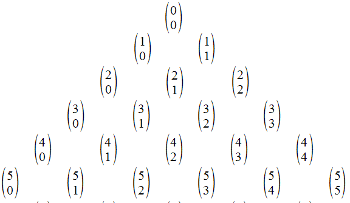
\includegraphics[scale=0.5]{img/2013-10-17/1} $\equiv$ 
\includegraphics[scale=0.5]{img/2013-10-17/2}

\subsection*{Anmerkung}
Binomialkoeffizienten sind wichtig in der Kombinatorik! \emph{(Stochastik)}

\section{\texorpdfstring{Satz: $k$-elementige Teilmengen}{Satz: k-elementige Teilmengen}}\label{2.9}
Die Anzahl der $k$-elementigen Teilmengen einer $n$-elementigen Menge ist $\bigbin{n}{k}$ ($n \in \N$)

\subsection*{Beispiel}
Beim Zahlenlotto ``6 aus 49'' werden $6$ aus $49$ nummerierten Kugeln gezogen ohne Zurücklegen.\\
Es gibt $\bigbin{49}{6} = 13.983.816$ mögliche Ziehungen.\\
Die Wahrscheinlichkeit für ``6 Richtige'' ist also rund: $\frac{1}{14.000.000}$\newpage %V2
% Kopfzeile beim Kapitelanfang:
\fancypagestyle{plain}{
%Kopfzeile links bzw. innen
\fancyhead[L]{\Large Vorlesung 3 (21.10.2013)}
%Kopfzeile rechts bzw. außen
\fancyhead[R]{}}
%Kopfzeile links bzw. innen
\fancyhead[L]{\Large Vorlesung 3 (21.10.2013)}
%Kopfzeile rechts bzw. außen
\fancyhead[R]{}
% **************************************************

\subsection*{Folgerung}
$\bigbin{n}{k} \in \N_0$ für $1 \le k \le n$

\subsection*{Beweis}
Ziehe $k$ Kugeln aus einer Urne mit $n$ nummerierten Kugeln ohne Zurücklegen (zunächst unter Beachtung der Reihenfolge):\nl
1. Zug: $n$ Möglichkeiten\\
2. Zug: $n-1$ Möglichkeiten\\
$k$. Zug: $n-k+1$ Möglichkeiten\nl
Insgesamt: $n \cdot (n-1) \cdot \hdots \cdot (n-k+1)$ Möglichkeiten\nl
Nach \emph{Satz 2.6} kommt dabei jede $k$-elementige Teilmenge in $k!$ verschiedenen Anordnungen vor (Reihenfolge der Kugeln).\nl
$\Rightarrow$ Die Anzahl der $k$-elementigen Teilmengen ist: $\frac{n \cdot {n-1} \cdot \hdots \cdot (n-k+1)}{k!} = \bigbin{n}{k}$ \qed

\subsection*{Wichtige Anwendung}\label{binFormel}
Seien $x,y \in \R$ und $n \in \N_0$.\\
Was ist dann $(x+y)^n$?\nl
$(x+y)^0=1$ (per Definition)\\
$(x+y)^1=x+y$\\
$(x+y)^2=x^2+2xy+y^2$ (Binomische Formel)\\
$(x+y)^3=x^3+3x^2y+3xy^2+y^3$\nl
Vermutung: Die Koeffizienten sind gerade Binomialkoeffizienten.

\newpage

\section{Binomischer Satz}\label{2.10}
Seien $x,y \in \R$ und $n \in \N_0$.\\
Dann ist \fbox{$(x+y)^n = \bigsum_{k=0}^n \bigbin{n}{k} x^k y^{n-k}$}\\
Insbesondere gilt für $y=1$: $(x+1)^n = \bigsum_{k=0}^n \bigbin{n}{k} x^k$

\subsection*{Beweis mit vollständiger Induktion}
\en{
\item Induktionsanfang: $n=0$\\
$(x+y)^0 = \bigbin{0}{0} x^0 y^0 = 1$ \ok
\item Induktionsvoraussetzung: Die Formel gilt für ein beliebiges, festes $n$.
\item Induktionsschluss: $n \rightarrow n+1$\\
$(x+y)^{n+1}=(x+y)\cdot(x+y)^n=(x+y)\cdot\left(\bigsum_{k=0}^n \bigbin{n}{k} x^k y^{n-k}\right)$\\
$=x \cdot \left(\bigsum_{k=0}^n \bigbin{n}{k} x^k y^{n-k}\right)+y \cdot \left(\bigsum_{k=0}^n \bigbin{n}{k} x^k y^{n-k}\right)$\\
$=\bigsum_{k=0}^n \bigbin{n}{k} x^{k+1} y^{n-k} + \bigsum_{k=0}^n \bigbin{n}{k} x^k y^{n-k+1}$\\
$=\bigsum_{k=1}^{n+1} \bigbin{n}{k-1} x^k y^{n-(k-1)} + \bigsum_{k=0}^n \bigbin{n}{k} x^k y^{n-k+1}$\\
$=\underbrace{y^{n+1}}_{k=0} + \underbrace{x^{n+1}}_{k=n+1} + \bigsum_{k=1}^n \underbrace{\left(\bigbin{n}{k} + \bigbin{n}{k-1}\right)}_{\bigbin{n+1}{k}} x^k y^{n+1-k}$\\
$=\bigsum_{k=0}^{n+1} \bigbin{n+1}{k} x^k y^{n+1-k}$ \ok
}
\qed

\newpage

\chapter{Die reellen Zahlen}\label{P3}
Ein Ziel bei der Erweiterung von Zahlenbereichen ist die Lösbarkeit von Gleichungen.\\
$\N \rightarrow \Z$: Löse $x+n=m$ mit $n,m \in \N_0$\\
$\Z \rightarrow \Q$: Löse $x \cdot n=m$ mit $n,m \in \Z$ und $n \neq 0$\\
Aber: $x^n=m$ mit $n,m \in \N$ hat in der Regel keine Lösung in $\Q$!

\section*{Beispiel (aus der Zentralübung)}
Es gibt kein $x \in \Q$ für $x^2=2$.\\
Abhilfe: Erweiterung $\Q \rightarrow \R$ (reelle Zahlen).\\
Im $\R$ hat $x^2=2$ zwei Lösungen: $x=\pm \sqrt{2}$

\section*{Axiomatische Einführung des reellen Zahlenraums}\label{AxiomeReelleZahlen}
\emph{(geht zurück auf \href{https://de.wikipedia.org/wiki/David_Hilbert}{David Hilbert})}\nl
Wir geben eine Reihe von grundlegenden Eigenschaften für $\R$ an:
\en{
\item Körperaxiome
\item Anordnungsaxiome
\item Vollständigkeitsaxiom (sichert u.a. die Lösbarkeit von $x^n=m$ mit $n,m \in \N$ ab)
}
Das Körper- sowie das Anordnungsaxiom werden übrigens auch von $\Q$ erfüllt.\nl
Man kann zeigen (wichtiger Satz), dass es genau eine Menge $\R$ mit diesen Eigenschaften (bis auf Umbenennungen) gibt.\\
Es gibt präzise Konstruktionen $\N \rightarrow \Z \rightarrow \Q \rightarrow \R$ so dass $\N \subset \Z \subset \Q \subset \R$ ist.

\section{Vorbemerkung: Quantoren}\label{3.1}
Gegeben seien Aussagen $P(x)$ mit $x \in X$ ($X$ sei eine Menge),\\
z.B. $X=\N$ und $P(x)=x \text{ ist gerade}$.\nl
\begin{tabular}{c|c}
Aussage & Schreibweise \\ 
\hline 
Für alle $x \in X$ gilt $P(x)$ & $\forall x \in X : P(x)$\\
Es gibt mindestens ein $x \in X$ mit $P(x)$ & $\exists x \in X : P(x)$\\
Es gibt genau ein $x \in X$ mit $P(x)$ & $\exists! x \in X : P(x)$\\
Es gibt kein $x \in X$ mit $P(x)$ & $\nexists x \in X : P(x)$
\end{tabular}\nl
Aus dem Vorwort wissen wir: $\forall$ ist der Allquantor, $\exists$ der Existenzquantor.

\subsection*{Beispiele}
$\exists n \in \N : n \ge 2$, $\nexists x \in \Q : x^2 = 2$, $\forall x \in \Q \exists n \in \N : x \cdot n \in \Z$

\newpage

\phantomsection
\addcontentsline{toc}{section}{Definition: Körperaxiome}
\section*{Definition: Körperaxiome}\label{Koerperaxiome}
Auf der Menge $\R$ sind zwei Rechenoperationen $+$ (die Addition) und $\cdot$ (die Multiplikation) erklärt, so dass $(\R, +, \cdot)$ ein Körper ist.

\section{Definition: Körper}\label{3.2}
Ein Körper ist eine Menge $K$ mit zwei Operationen $+$ und $\cdot$, so dass gilt:
\begin{enumerate}[label=(K\arabic*)]
\item Assoziativgesetz:\\
$\forall x,y,z \in K : (x+y)+z = x+(y+z)$ (Assoziativität für die Addition)\\
$\forall x,y,z \in K : (x \cdot y) \cdot z = x \cdot (y \cdot z)$ (Assoziativität für die Multiplikation)
\item Kommutativgesetz:\\
$\forall x,y \in K : x+y = y+x$ (Kommutativität für die Addition)\\
$\forall x,y \in K : x \cdot y = y \cdot x$ (Kommutativität für die Multiplikation)
\item Existenz neutraler Elemente:\\
$\forall x \in K \exists 0 \in K : x+0 = x$ (Nullelement)\\
$\forall x \in K \exists 1 \in K : x \cdot 1 = x$ (Einselement)
\item Existenz von Inversen:\\
$\forall x \in K \exists y \in K : x+y = 0$ (additives Inverses von $x$)\\
$\forall x \in K \setminus \{0\} \exists z \in K : x \cdot z = 1$ (multiplikatives Inverses von $x$)
\item Distributivgesetz:\\
$\forall x,y,z \in K : x \cdot (y+z) = x \cdot y + x \cdot z$
\end{enumerate}

\subsection*{Anmerkung}
Jedem Paar $(x,y) \in K \times K$ wird genau ein Element $x+y \in K$ bzw. $x \cdot y = xy \in K$ zugeordnet.

\section{Folgerungen}\label{3.3}
Sei $K$ ein Körper.
\en{
\item $0$ und $1$ sind eindeutig bestimmt.\\
Beweis für $0$ (für $1$ analog): Sei auch $0'$ neutral bezüglich der Addition.\\
$\Rightarrow 0=0+0' \underset{K2}{=} 0'+0 \underset{K3}{=} 0'$
\item $y$ und $z$ in (K4) sind (bei festem $x$) eindeutig bestimmt.\\
Beweis für $y$ (Addition): Sei $x+y'=0=x+y$\\
$\Rightarrow y \underset{K3}{=} y+0 = y+(x+y') \underset{K1}{=} (y+x)+y' \underset{K2}{=} (x+y)+y' = 0+y' \underset{K2}{=} y'$\\
Bezeichnung: $-x$ ist das additive Inverse von $x$ und $x^{-1} = \frac{1}{x}$ das multiplikative Inverse von $x \neq 0$
\item $a,b \in K \Rightarrow$ die Gleichung $a+x=b$ hat eine eindeutige Lösung $x=b+(-a) =: b-a$\\
Falls $a \neq 0 \Rightarrow$ auch $a \cdot x = b$ hat eine eindeutige Lösung $x=a^{-1} \cdot b =: \frac{b}{a}$\\
Beweis für die Addition: $a+x=b \Leftrightarrow a+x+(-a)=b+(-a) \Leftrightarrow (a+(-a))+x=b-a \Leftrightarrow x=b-a$\\
Analog für die Multiplikation.
\item $-(-x)=x$ und falls $x \neq 0$ gilt: $(x^{-1})^{-1}=x$\\
Beweis für das additive Inverse: $(-x)+x \underset{K2}{=} x+(-x)=0 \underset{K2}{\Rightarrow} -(-x)$
\item $-(x+y)=-x-y$ und falls $x,y \neq 0$ gilt: $(xy)^{-1} = x^{-1} y^{-1}$ (Beweis in Übung)
\item $\forall x \in K : x \cdot 0 = 0$\\
Denn: $\frac{x \cdot 0}{a}+x \cdot 0 = x \cdot (0+0) = \frac{x \cdot 0}{b} \Rightarrow x \cdot 0 = x \cdot 0 - x \cdot 0 = 0$
\item $xy = 0 \Leftrightarrow x=0 \vee y=0$
\item $(-x)y=-xy$\\
Insbesondere: $(-1)y=-y$
}
Beweise von 7. und 8. in der Übung.\newpage %V3
% Kopfzeile beim Kapitelanfang:
\fancypagestyle{plain}{
%Kopfzeile links bzw. innen
\fancyhead[L]{\Large Vorlesung 4 (24.10.2013)}
%Kopfzeile rechts bzw. außen
\fancyhead[R]{}}
%Kopfzeile links bzw. innen
\fancyhead[L]{\Large Vorlesung 4 (24.10.2013)}
%Kopfzeile rechts bzw. außen
\fancyhead[R]{}
% **************************************************
\phantomsection
\addcontentsline{toc}{section}{Allgemeines Assoziativ- und Kommunitativgesetz}
\section*{Allgemeines Assoziativ- und Kommunitativgesetz}
$x_1+x_2+\hdots+x_n := (\hdots((x_1+x_2)+x_3)+\hdots)$\\
Wiederholte Anwendung des A- und K-Gesetzes zeigt: Das Eregbnis ist unabhängig von Klammerung (also Klammern weglassen!) und Reihefolge.\\
Das gilt auch für Produkte.

\section*{Potenzen}
Sei $x \in K$.\\
Für $n \in \N$ setze $x^n := \underbrace{x \cdot x \cdot \hdots \cdot x}_{n \text{ Faktoren}}$ mit $x^0=1$\\
Falls $x \neq 0$ setze $x^{-1} := (x^{-1})^n$\\
Damit: $x^{-n} = (x^n)^{-1}$\\
Regeln für $x,y \in K$ und $n,m \in \N_0$ seien:
\items{
\item $x^n x^m = x^{n+m}$
\item $x^n y^n = (xy)^n$
\item $(x^n)^m = x^{nm}$
}
Falls $x,y \neq 0$ gelten diese Regeln auch für alle $n,m \in \Z$.

\subsection*{Beispiele}
$\R$ und $\Q$ sind Körper mit den üblichen Operationen.\\
$\Z$ ist kein Körper, denn nur $+1$ und $-1$ haben multiplikative Inverse.

\subsection*{Beispiel eines endlichen Körpers}\label{BspEndlKoerper}
$\F_2=\{0,1\}$ mit Operationen wie folgt:\nl
\begin{tabular}{c|c|c}
$+$ & $0$ & $1$ \\ 
\hline 
$0$ & $0$ & $1$\\
$1$ & $1$ & $0$
\end{tabular}\hspace{5em}
\begin{tabular}{c|c|c}
$\cdot$ & $0$ & $1$ \\ 
\hline 
$0$ & $0$ & $0$\\
$1$ & $0$ & $1$
\end{tabular}\nl
Nachweis des Axioms: direktes Nachprüfen.\\
In $\F_2$ gilt: $1+1=0$

\newpage

\phantomsection
\addcontentsline{toc}{section}{Definition: Anordnungsaxiome}
\section*{Definition: Anordnungsaxiome}\label{Anordnungsaxiome}
$\R$ enthält eine Teilmenge von Elementen, die als positiv ausgezeichnet sind (Schreibweise: $x>0$).
\begin{enumerate}[label=(A\arabic*)]
\item Jedes $x \in \R$ genügt genau eine der Beziehungen $x>0$, $x=0$, $-x>0$ (Trichotomie)
\item $x>0 \wedge y>0 \Rightarrow x+y>0, x \cdot y > 0$
\end{enumerate}

\subsection*{Beziehungen}
$x>y \Leftrightarrow x-y>0$\\
$x<y \Leftrightarrow y>x$\\
$x \ge y \Leftrightarrow x>y \vee x=y$\\
$x \le y \Leftrightarrow y \ge x$

\section{Folgerungen}\label{3.4}
\en{
\item $x<0 \Leftrightarrow -x>0$
\item $\forall x,y \in \R$ gilt genau eine der Beziehungen $x>y, x=y, x<y$
\item $x<y \wedge y<z \Rightarrow x<z$ (Transitivität)
\item $x<y, z \in \R \Rightarrow x+z<y+z$ 
\item $x<y \Leftrightarrow -y < -x$
\item $x<y \wedge a < b \Rightarrow x+a < y+b$
\item $x<y \wedge a > 0 \Rightarrow ax < ay$ (i)\\
$x<y \wedge a < 0 \Rightarrow ax > ay$ (ii)
\item $0 \le x < y, 0 \le a < b \Rightarrow ax < by$\\
Folgerung (mit $a=x, b=y$): $0 \le x < y \Rightarrow x^2 < y^2 \Rightarrow x^n < y^n$ ($\forall n \in \N$)
\item $x \neq 0 \Rightarrow x^2 > 0$, insbesondere $1=1 \cdot 1 > 0$
}

\subsection*{Beweise}
\en{
\item $x<0 \Leftrightarrow 0>x \Leftrightarrow 0-x=-x>0$
\item aus Trichotomie für $x-y$
\item $z-x=(z-y)+(y-x)>0$
\item bilde Differenz
\item bilde Differenz
\item $(y+b)-(x+a)=\underbrace{(y-x)}_{>0} + \underbrace{(b-a)}_{>0} > 0$
\item (i) $ay-ax=\underbrace{a}_{>0} \underbrace{(y-x)}_{>0} > 0$\\
(ii) $a<0 \Rightarrow -a>0$ analog
\item In der Übung
\item Falls $x>0$: $\Rightarrow x^2>0$\\
Falls $x<0$: $\Rightarrow [\text{7.(ii) mit }y=0, a=x]\,x^2>0$
}

\newpage

\section{Definition: Angeordnete Körper}\label{3.5}
Ein Körper $K$, in dem eine Teilmenge von Elementen als positiv ausgezeichnet ist ($x>0$), so dass die Axiome (A1) und (A2) gelten, heißt \underline{angeordneter Körper}.\\
Die Folgerungen 3.5 gelten in jedem angeordneten Körper.\nl
$\R$ und $\Q$ sind angeordnete Körper.\\
$\F_2$ ist kein angeordneter Körper, denn in $\F_2$ gilt: $1+1=0$\\
Annahme: $\F_2$ wäre angeordnet. $\Rightarrow 1>0 \Rightarrow 1+1 > 0$ \wspruch

\section{Bernoulli-Ungleichung}\label{3.6}
Sei $x \in \R$, $x>-1$ und $n \in \N_0$.\\
Dann ist $(1+x)^n \ge 1+nx$.

\subsection*{Beweis mit vollständiger Induktion}
\en{
\item Induktionsanfang: $n=0$\\
$(1+x)^0 = 1 = 1+0 \cdot x$ \ok
\item Induktionsvoraussetzung: Die Bernoulli-Ungleichung gelte für ein beliebiges, festes $n$.
\item Induktionsschluss: $n \rightarrow n+1$\\
$(1+x)^{n+1} = \underbrace{(1+x)}_{>0} \cdot \underbrace{(1+x)^n}_{>=1 \text{ nach IV}} \ge (1+x) \cdot (1+nx)$\\
$=1+(n+1)x+nx^2 \ge 1+(n+1)x$ \ok
}
\qed

\section{Definition: Betrag}\label{3.7}
Sei $x \in \R$.\\
$|x| := \left\{
\begin{array}{l l}
x & \quad \text{falls } x \ge 0\\
-x & \quad \text{falls } x<0
\end{array} \right.$\\
Insbesondere: $|x| \ge 0$ und $|-x|=|x|$\\
Anschaulich: $|x|$ ist der Abstand von $x$ und $-x$ zu $0$.\\
\begin{tikzpicture}[decoration=brace]
% Die Grundlinie:
\draw(0,0)--(5,0);
\foreach \x/\xtext in {0.5/$-x$,2.5/$0$,4.5/$x$}
  \draw(\x,5pt)--(\x,-5pt) node[below] {\xtext};
\draw[decorate, yshift=2ex]  (0.5,0) -- node[above=0.4ex] {$|x|$}  (2.5,0);
\draw[decorate, yshift=2ex]  (2.5,0) -- node[above=0.4ex] {$|x|$}  (4.5,0);
\end{tikzpicture}

\newpage

\section{Satz: Regeln für Beträge}\label{3.8}
\en{
\item $|x| \ge 0$ wohei $|x|=0 \Leftrightarrow x=0$
\item $|xy| = |x| \cdot |y|$ (Multiplikativität)
\item $\left| \frac{x}{y} \right| = \frac{|x|}{|y|}$ falls $y \neq 0$
\item $|x+y| \le |x|+|y|$ (Dreiecksungleichung)
}

\subsection*{Beweise}
\en{
\item Klar aus Definition \ok
\item $|xy| \in \{\pm xy\}, |x| \cdot |y| \in \{\pm xy\}$\\
Beide sind $\ge 0 \Rightarrow$ Gleichheit \ok
\item $x=\frac{x}{y} \cdot y \Rightarrow |x|=\left|\frac{x}{y}\right| \cdot \underbrace{|y|}_{\neq 0} \Rightarrow$ Behauptung \ok
\item $\pm x\le|x|, \pm y\le|y| \Rightarrow \pm(x+y)\le|x|+|y| \Rightarrow$ Behauptung \ok
}
\qed

\phantomsection
\addcontentsline{toc}{section}{Intervalle}
\section*{Intervalle}\label{Intervalle}
Seien $a,b \in \R$ mit $a \le b$.
\en{
\item Abgeschlossenes Intervall: $[a,b] := \{x \in \R : a \le x \le b\}$\\
\begin{tikzpicture}[decoration=brace]
\draw[->](0,0)--(5,0);
\foreach \x/\xtext in {0.5/$a$,2.5/$x$,4.5/$b$}
  \draw(\x,-5pt) node[below] {\xtext};
\draw(0.5,0pt) node{[};
\draw(4.5,0pt) node{]};
\end{tikzpicture}
\item Offenes Intervall: $(a,b) := \{x \in \R : a < x < b\}$\\
\begin{tikzpicture}[decoration=brace]
\draw[->](0,0)--(5,0);
\foreach \x/\xtext in {0.5/$a$,2.5/$x$,4.5/$b$}
  \draw(\x,-5pt) node[below] {\xtext};
\draw(0.5,0pt) node{(};
\draw(4.5,0pt) node{)};
\end{tikzpicture}
\item Halboffene Intervalle: $[a,b) := \{x \in \R : a \le x < b\}$ und $(a,b] := \{x \in \R : a < x \le b\}$\\
\begin{tikzpicture}[decoration=brace]
\draw[->](0,0)--(5,0);
\foreach \x/\xtext in {0.5/$a$,2.5/$x$,4.5/$b$}
  \draw(\x,-5pt) node[below] {\xtext};
\draw(0.5,0pt) node{[};
\draw(4.5,0pt) node{)};
\end{tikzpicture}
\begin{tikzpicture}[decoration=brace]
\draw[->](0,0)--(5,0);
\foreach \x/\xtext in {0.5/$a$,2.5/$x$,4.5/$b$}
  \draw(\x,-5pt) node[below] {\xtext};
\draw(0.5,0pt) node{(};
\draw(4.5,0pt) node{]};
\end{tikzpicture}
\item Uneigentliche Intervalle: $[a,\infty) := \{x \in \R : x \ge a\}$ und $(\infty,a] := \{x \in \R : x \le a\}$\\
\begin{tikzpicture}[decoration=brace]
\draw[->](0,0)--(5,0);
\foreach \x/\xtext in {0.5/$a$}
  \draw(\x,-5pt) node[below] {\xtext};
\draw(0.5,0pt) node{[};
\end{tikzpicture}
\begin{tikzpicture}[decoration=brace]
\draw[->](0,0)--(5,0);
\foreach \x/\xtext in {4.5/$a$}
  \draw(\x,-5pt) node[below] {\xtext};
\draw(4.5,0pt) node{]};
\end{tikzpicture}
}

\newpage

\section{Definition: Vollständigkeitsaxiom}\label{3.9}
\emph{In eckigen Klammern stehendes bezieht sich auf ``nach unten beschränkt''}\nl
$M \subseteq \R$ heißt \underline{nach oben [unten] beschränkt} $\Leftrightarrow \exists s \in \R : x \le s \forall x \in M$ [$x \ge s \forall x \in M$]\\
Das $s$ ist dann die \underline{obere [untere] Schranke von $M$}.\\
Eine obere [untere] Schranke, die in $M$ liegt, ist das \underline{Maximum [Minimum] von $M$}.\\
$M$ heißt \underline{beschränkt} $\Leftrightarrow M$ ist nach oben \underline{und} unten beschränkt.\\
\begin{tikzpicture}[decoration=brace]
\draw[->](0,0)--(5,0);
\foreach \x/\xtext in {0.75/$t$,2.5/$M$,4.25/$s$}
  \draw(\x,-5pt) node[below] {\xtext};
\draw(1.5,0pt) node {$|$};
\draw(3.5,0pt) node {$|$};
\end{tikzpicture}

\subsection*{Beispiele}
\en{
\item $M=[0,1] \Rightarrow M$ ist beschränkt.\\
Jedes $s \ge 1$ ist obere Schranke und jedes $t \le 0$ ist untere Schranke von $M$.\\
$1$ ist Maximum, $0$ ist Minimum von $M$ ($1=\text{max }M$ und $0=\text{min }M$).
\item $M=[0,1)$\\
$M$ hat kein Maximum, denn es gibt kein $m \in [0,1)$, welches obere Schranke des Intervalls ist.\\
Es gibt immer größere Zahlen, die sich auch im Intervall befinden. ($m < \underbrace{\frac{1}{2}(m+1)}_{\in [0,1)} < 1$)
\item Das Intervall, das zur linken Seite geöffnet ist, hat kein Minimum (analog).
}\newpage %V4
% Kopfzeile beim Kapitelanfang:
\fancypagestyle{plain}{
%Kopfzeile links bzw. innen
\fancyhead[L]{\Large Vorlesung 5 (28.10.2013)}
%Kopfzeile rechts bzw. außen
\fancyhead[R]{}}
%Kopfzeile links bzw. innen
\fancyhead[L]{\Large Vorlesung 5 (28.10.2013)}
%Kopfzeile rechts bzw. außen
\fancyhead[R]{}
% **************************************************
\section{Definition: Supremum, Infimum}\label{3.10}
Sei $M \subseteq \R$.
\en{
\item $s \in \R$ heißt \underline{Supremum von $M$} $\Leftrightarrow s$ ist kleinste obere Schranke von $M$.\\
Das heißt:
\begin{enumerate}[label=\roman*.]
\item $s$ ist obere Schranke von $M$.
\item $s \le s'$ für jede weitere obere Schranke $s'$ von $M$.
\end{enumerate}
\item $t \in \R$ heißt \underline{Infimum von $M$} $\Leftrightarrow t$ ist größte untere Schranke von $M$.
}
1.ii. zeigt: $M$ hat höchstens ein Supremum $s$ (bezeichnet mit $s = \text{sup } M$),\\
denn: $s, s'$ seien Suprema $\Rightarrow s \le s' \wedge s' \le s \Rightarrow s=s'$\\
Analog: $M$ hat höchstens ein Infimum $t$ (bezeichnet mit $t = \text{inf } M$).

\subsection*{Beispiel}
$M = [0,1] \Rightarrow 1 = \text{sup } M$ (denn: $1$ ist obere Schranke, und kein $x<1$ ist obere Schranke).

\section{\texorpdfstring{Vollständigkeitsaxiom: Supremumseigenschaft von $\R$}{Vollständigkeitsaxiom: Supremumseigenschaft von \R}}\label{3.11}
Sei $M \subseteq \R, M \neq \emptyset$ nach oben beschränkt $\Rightarrow M$ besitzt ein Supremum.

\section{\texorpdfstring{Folgerung aus der Supremumseigenschaft von $\R$}{Folgerung aus der Supremumseigenschaft von \R}}\label{3.12}
Sei $M \subseteq \R, M \neq \emptyset$ nach unten beschränkt $\Rightarrow M$ beistzt ein Infimum.\\
Betrachte $-M = \{-x : x \in M\}$. $-M$ hat ein Supremum $s$, da es nach oben beschränkt ist.\\
Also hat $M$ ein Infimum $-s$.\nl
\begin{tikzpicture}[decoration=brace]
\draw(0,0)--(5,0);
\foreach \x/\xtext in {1.5/$s$,2.5/$0$,3.5/$-s$}
  \draw(\x,-5pt) node[below] {\xtext};
\draw(2.5,0pt) node{$|$};
\draw(1.5,0pt) node{)};
\draw(3.5,0pt) node{(};
\draw(0.75,7pt) node{$-M$};
\draw(4.25,7pt) node{$M$};
\end{tikzpicture}

\subsection*{Beispiel}
$M=(-3,2] \Rightarrow \text{inf } M = -3$

\subsection*{Beachte}
Hat $M$ ein Maximum $m=\text{max } M$, so ist zugleich $m=\text{sup } M$,\\
denn: $x<m \Rightarrow x \text{ ist keine obere Schranke für } M$.

\section{Lemma}\label{3.13}
Sei $M \subseteq \R, M \neq \es$ nach oben beschränkt und $s = \text{sup }M$.\\
$\Rightarrow \forall \eps>0 \exists x \in M:s-\eps<x \le s$

\subsection*{Beweis}
$s-\eps$ ist keine obere Schranke von $M$ (da $s$ schon die kleinste obere Schranke ist).\\
$\Rightarrow \exists x \in M:s-\eps<x$ Dabei ist $x \le s$, da obere Schranke von $M$. \qed

\section{\texorpdfstring{Satz: Archimedische Eigenschaft von $\R$}{Satz: Archimedische Eigenschaft von \R}}\label{3.14}
\begin{enumerate}[label=(AR)]
\item $\forall x \in \R \exists n \in \N : n > x$\\
\begin{tikzpicture}[decoration=brace]
\draw[->](0,0)--(5,0);
\foreach \x/\xtext in {1.5/$0$,3.5/$x$,4.5/$n$}
  \draw(\x,-5pt) node[below] {\xtext};
\draw(1.5,0pt) node{$|$};
\draw(3.5,0pt) node{$|$};
\draw(4.5,0pt) node{$|$};
\end{tikzpicture}
\end{enumerate}

\subsection*{Beweis durch Widerspruch}
Angenommen, (AR)  gelte nicht, also:\\
$\exists x \in \R : n \le x \forall n \in \N$\\
$\Rightarrow \N$ ist (durch $x$) nach oben beschränkt $\Rightarrow s = \text{sup } \N$ existiert.\\
$\Rightarrow$ (nach Lemma 3.13) $\exists n \in \N : s-1 < n$ ($\eps = 1$)\\
$\Rightarrow \underbrace{n+1}_{\in \N} > s$ \wspruch \qed

\section{\texorpdfstring{Folgerungen aus der archimedischen Eigenschaft von $\R$}{Folgerungen aus der archimedischen Eigenschaft von \R}}\label{3.15}
\en{
\item $\forall \eps > 0 \exists n \in \N : \frac{1}{n} < \eps$
\item Wachstum von Potenzen:\\
Sei $a \in \R, a > 1 \Rightarrow \forall M > 0 \exists n \in \N : a^n > M$
\item Sei $a \in \R, 0 < a < 1 \Rightarrow \forall \eps > 0 \exists n \in \N : a^n < \eps$\\
\begin{tikzpicture}[decoration=brace]
\draw[->](0,0)--(5,0);
\foreach \x/\xtext in {0.0/$0$,0.5/$a^n$,1.0/$\eps$,3.5/$a$,4.5/$1$}
  \draw(\x,-5pt) node[below] {\xtext} (\x,0pt) node{$|$};
\end{tikzpicture}
}

\subsection*{Beweis}
\en{
\item Sei $\eps > 0$. Dann: (AR) $\Rightarrow \exists n \in \N : n > \frac{1}{\eps} \Rightarrow \frac{1}{n} < \eps$
\item Sei $M>0$. $x = a-1 > 0 \Rightarrow a^n=(1+x)^n > 1+nx > nx \forall n \in \N$\\
(AR) $\Rightarrow \exists n \in \N : n > \frac{M}{x} \Rightarrow a^n > M$
\item Sei $\eps>0$. $\frac{1}{a}>1 \underset{\text{(2)}}{\Rightarrow} \exists n \in \N : \left(\frac{1}{a}\right)^n > \frac{1}{\eps} \Rightarrow a^n < \eps$
} \qed \nl
Man kann sagen: Es gibt (bis auf Umbenennungen) genau einen angeordneten Körper,\\
der das Vollständigkeitsaxiom erfüllt, nämlich $\R$.

\newpage

\section*{\texorpdfstring{Wichtige Konsequenz der Vollständigkeit von $\R$:}{Wichtige Konsequenz der Vollständigkeit von \R:}}
\section{Satz: Existenz von Wurzeln}\label{3.16}
Sei $a \in \R, a \ge 0$ mit $k \in \N \Rightarrow \exists! x \in \R , x \ge 0 : x^k = a$

\subsection*{Schreibweise}
$x=a^{\frac{1}{k}} = \sqrt[k]{a}$ (sprich: $k$-te Wurzel aus $a$)\\
$\sqrt[2]{a} = \sqrt{a}$

\subsection*{Beachte}
$\sqrt[k]{0}=0$ und $\forall a>0$ ist $\sqrt[k]{a}>0$ (per Definition)

\subsection*{Beweis}
\en{
\item \underline{Eindeutigkeit}:\\
Seien $x_1 , x_2 \ge 0, x_1 \neq x_2$ mit $x_1^k = a = x_2^k$.
Sei etwa $x_1 < x_2 \underset{\text{3.4}}{\Rightarrow} x_1^k < x_2^k$ \wspruch
\item \underline{Existenz}:\\
Hier für $k=2$ ($k>2$ ähnlich, etwas aufwendiger).\\
Sei ohne Einschränkung \emph{(kurz: o.e.)} $a \ge 1$.\\
(Für $a=0$ klar; für $0<a<1$ betrachten wir den Kehrwert $\frac{1}{a}>1$.\\
Ist $y^k = \frac{1}{a} \underset{y \neq 0}{\Rightarrow} (\frac{1}{y})^k = a$)\\
Setze $M := \{y>0 : y^2 \le a\}$. $M \neq \es$ (da $1 \in M$) ist nach oben beschränkt durch $a$, denn:\\
Angenommen, $\exists y \in M : y > a \Rightarrow y^2 > a^2 \underset{a \ge 1}{\ge} a$. \wspruch \\
Setze $x := $ sup $M$.\nl
\underline{Behauptung}: $x^2=a$\\
\underline{Annahme 1}: $x^2 > a \Rightarrow \eps := \frac{x^2-a}{2x} > 0$\\
\begin{tikzpicture}[decoration=brace]
\draw[->](0,0)--(5,0);
\foreach \x/\xtext in {1.0/$x-\eps$,2.5/$y \in M$,4.0/$x$}
  \draw(\x,-5pt) node[below] {\xtext} (\x,0pt) node{$|$};
\end{tikzpicture}\\
Nach Lemma 3.13 $\Rightarrow \exists y \in M : x - \eps < y \le x$. Dabei $y^2 \le a$.\\
$x^2-a \le x^2 - y^2 = \underbrace{(x+y)}_{\in (0,2x]} \underbrace{(x-y)}_{\in [0,\eps)} < 2x \eps - x^2 - a$ \wspruch \\
\underline{Annahme 2}: $x^2 < a \Rightarrow \frac{1}{x^2} > 1 \Rightarrow \frac{a}{x^2} -1 > 0$\\
Sei $r := $ min $\left\{1, \frac{1}{3} \cdot \left(\frac{a}{x^2} - 1\right)\right\} > 0 \Rightarrow (1+r)^2 = 1+(2+r) \cdot r < 1 + 3r \le \frac{1}{x^2}$\\
$\Rightarrow (x(1+r))^2 \le a \Rightarrow x(1+r) \in M$, aber $x(1+r) > x$ (\wspruch zu $x=$ sup $M$!)
} \qed

\newpage

\section{Rechenregel für Wurzeln gleichen Exponents}\label{3.17}
Seien $x,y \in \R$ und $x,y > 0$ und $k \in \N \Rightarrow \sqrt[k]{x} \cdot \sqrt[k]{y} = \sqrt[k]{xy}$

\subsection*{Beweis}
$\left(\sqrt[k]{x} \cdot \sqrt[k]{y}\right)^k = \left(\sqrt[k]{x}\right)^k \cdot \left(\sqrt[k]{y}\right)^k = x \cdot y$ (Behauptung)\nl
Wir wissen: $\sqrt{2} \in \R \setminus \Q$. Also $\Q \subset \R \wedge \Q \neq \R$ ($\R$ ist bedeutend größer!).\\
Die Zahlen aus $\R \setminus \Q$ heißen irrational.

\subsection*{Bemerkung}
Im Körper $\Q$ ist das Vollständigkeitsaxiom \underline{nicht} erfüllt, das heißt es gibt beschränkte Mengen $M \subsetneq \Q$, so dass $M$ kein Supremum in $\Q$ hat.\\
Denn sonst würde 3.16 auch in $\Q$ gelten $\Rightarrow x^2=2$ hätte eine Lösung in $\Q$ \wspruch

\subsection*{Beispiel}
$\{y \in \Q : y > 0 \wedge y^2 \le 2 \}$ hat kein Supremum in $\Q$.

\newpage

\chapter{Funktionen}\label{P4}
\section{Definition: Funktionen, Abbildungen}\label{4.1}
Seien $X, Y$ Mengen. Eine \underline{Abbildung} \emph{(=Funktion)} $f$ von $X$ nach $Y$ ist eine Vorschrift, die jedem $x \in X$ genau ein $y=f(x) \in Y$ zuordnet.

\subsection*{Schreibweise}
$f: X \to Y, x \mapsto f(x)$\\
$X$: Definitionsbereich von $f$\\
$Y$: Ziel-, Wertebereich von $f$\\
$f(x)$: Bild von $x$ unter $f$ (Wert von $f$ in $x$)

\phantomsection
\addcontentsline{toc}{section}{Graph von f}
\section*{\texorpdfstring{Graph von $f$}{Graph von f}}
$\Gamma_f=\{(x,f(x)): x \in X\} \subseteq X \times Y$ \nl
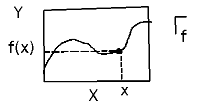
\includegraphics[scale=0.5]{img/2013-10-28/1}
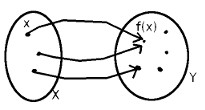
\includegraphics[scale=0.5]{img/2013-10-28/2}\\
Beachte: Bei jedem $x \in X$ (im rechten Bild) startet genau ein Pfeil!

\subsection*{Bezeichnung}
Der Begriff ``Funktion'' ist insbesondere gängig, falls $X$ und $Y$ Mengen von Zahlen sind.\newpage %V5
% Kopfzeile beim Kapitelanfang:
\fancypagestyle{plain}{
%Kopfzeile links bzw. innen
\fancyhead[L]{\Large Vorlesung 6 (31.10.2013)}
%Kopfzeile rechts bzw. außen
\fancyhead[R]{}}
%Kopfzeile links bzw. innen
\fancyhead[L]{\Large Vorlesung 6 (31.10.2013)}
%Kopfzeile rechts bzw. außen
\fancyhead[R]{}
% **************************************************
\subsection*{Beispiele}\label{BeispieleAbbildungen}
\en{
\item $X=\{$Studenten an der Uni Paderborn$\}, f: X \to \N, x \mapsto $ Alter von $x$
\item $f: \R \to \R, x \mapsto x^2$\\
$\Gamma_f:$ Normalparabel\\
$f(\R)=\{x \in \R, x>0\}$\\
Wenn einem $x \in X$ mehrere $y \in Y$ zugeordnet werden können, ist es keine Funktion!
\item \underline{Lineare Funktionen}:\\
$f: \R \to \R, x \mapsto ax+b$ ($a,b \in \R$)\\
$\Gamma_f$: Gerade, $a$: Steigung, $b$: Achsenabschnitt
\item \underline{Polynomfunktionen}:\\
Funktion der Form $p: \R \to \R, p(x)=a_n x^n + \hdots + a_1 x + a_0$\\
mit $n \in \N_0$ und $a_1 , \hdots , a_n \in \R$ Koeffizienten
\item \underline{Floorfunktion (Gauß-Klammer)}:\\
$\lfloor . \rfloor = \R \to \R$\\
$\lfloor x \rfloor :=$ größtes $k \in \Z$ mit $k \le x$
\item \underline{Identische Abbildung}:\\
$id_x: X \to X, x \mapsto x$
\item $P :=$ Menge aller Sortierprogramme für endliche Listen\\
$L: P \times \N \to \R$\\
$L(p,n) :=$ max. Laufzeit, die Programm $p$ zum Sortieren einer Liste der Länge $n$ braucht
}
Für die Charakterisierung einer Abbildung ist neben der Abbildungsvorschrift auf der Definitionsbereich $X$ wichtig.

\subsection*{Beispiel}
$f: \R \to \R, f(x)=|x|$ und $g: [-1,1] \to \R, g(x)=|x|$ sind verschiedene Abbildungen, denn $g$ ist eine Restriktion von $f$.

\section{Definition: Bild, Urbild}\label{4.2}
\begin{enumerate}[label=(\roman*)]
\item Sei $f: X \to Y$ eine Abbildung. Sei $A \subseteq X$.\\
$f(A) := \{f(x) : x \in A\}$ ist das \underline{Bild von $A$ unter $f$}.\\
$f(X) \subseteq Y$ ist der Wertebereich von $f$.
\item Sei $B \subseteq Y$.\\
$f^{-1}(B) := \{x \in X : f(x) \in B\}$ ist das \underline{Urbild von $B$ unter $f$}.\\
$f^{-1}$ ist hierbei \underline{keine} eigenständige Funktion, sondern nur eine Bezeichnung!
\end{enumerate}

\subsection*{Beispiel}
$f: \Z \to \Z: x \mapsto x^2$\\
$f(\{-2,5\})=\{4,25\}$\\
$f^{-1}(\{4,25\})=\{\pm 2,\pm 5\}$\\
$f^{-1}(\{3\})=\es$\\
$f^{-1}(\{4\})=\{\pm 2\}$\\
$f^{-1}(\{3,4\})=\{\pm 2\}$

\newpage

\section{Definition: Komposition von Abbildungen}\label{4.3}
Seien $f: X \to Y$ und $g: Y \to Z$ Abbildungen.\\
Die Komposition (Verknüpfung, Verkettung) von $f$ und $g$ ist die Abbildung:\\
$g \circ f: X \to Z, x \mapsto g(f(x))$ ($g$ nach $f$)

\subsection*{Beispiel}
$f,g : \R \to \R, f(x)=2x+1, g(x)=x^2$\\
$\left. \begin{array}{l}
(g \circ f)(x) = (2x+1)^2=4x^2+4x+1\\
(f \circ g)(x) = 2x^2+1
\end{array} \right \} \Rightarrow f \circ g \neq g \circ f$

\section{Satz: Assoziativität der Komposition}\label{4.4}
Seien $f: X \to Y$, $g: Y \to Z$ und $h: Z \to W$ Abbildungen.\\
$\Rightarrow h \circ (g \circ f) = (h \circ g) \circ f$

\subsection*{Beweis}
$(h \circ (g \circ f))(x)=h((g \circ f)(x))=h(g(f(x)))=((h \circ g) \circ f)(x)$ \qed

\section{Definition: Eigenschaften von Abbildungen (Injektivität, Surjektivität, Bijektivität)}\label{4.5}
$f: X \to Y$ heißt:
\en{
\item \underline{injektiv}, falls es zu jedem $y \in Y$ \underline{höchstens} ein $x \in X$ gibt mit $f(x)=y$
\item \underline{surjektiv}, falls es zu jedem $y \in Y$ \underline{mindestens} ein $x \in X$ gibt mit $f(x)=y$
\item \underline{bijektiv}, falls $f$ sowohl injektiv als auch surjektiv ist, also falls es zu jedem $y \in Y$ \underline{genau} ein $x \in X$ gibt mit $f(x)=y$
}

\subsection*{Also}
$f$ injektiv $\Leftrightarrow \forall x_1, x_2 \in X$ gilt: wenn $f(x_1)=f(x_2)$ dann $x_1=x_2$\\
$f$ surjektiv $\Leftrightarrow \forall y \in Y \exists x \in X: y=f(x) \Leftrightarrow f(X)=Y$\\
$f$ bijektiv $\Leftrightarrow \forall y \in Y \exists! x \in X: y=f(x)$

\subsection*{Anmerkungen zur Hausübung}
$2^n-1$ prim $\Rightarrow n$ prim\\
Beweis durch Widerspruch:\\
Angenommen, $n=pq$ und $p,q \neq 1$\\
$2^n-1=2^{pq}-1=(\underbrace{2^p}_{x})^q -1=x^q -1$

\newpage

\subsection*{Beispiele}
$f: \N \to \N$ drei Varianten:
\begin{enumerate}[label=(\roman*)]
\item $f(n)=n+1$ ist injektiv, aber nicht surjektiv
\item $f(n)=\left\{ \begin{array}{l l}
1 & \text{falls } n=1 \\
n-1 & \text{falls } n \ge 2
\end{array} \right.$ ist surjektiv, aber nicht injektiv
\item $f(n)=\left\{ \begin{array}{l l}
n-1 & \text{falls } n \text{ gerade} \\
n+1 & \text{falls } n \text{ ungerade}
\end{array} \right.$ ist bijektiv
\end{enumerate}
Sei $f:X \to Y$ bijektiv, das heißt $\forall y \in Y \exists! x \in X : f(x)=y$.\\
Wir können dann $g: Y \to X$ definieren durch: $g(y) := x$ falls $y=f(x)$.\\
Damit ist $g(f(x))=x \forall x \in X$ und $f(g(y)) = y \forall y \in Y$.\\
Das heißt: $g \circ f = id_x$ und $f \circ g = id_y$.

\section{Definition: Umkehrabbildung}\label{4.6}
$g$ heißt \underline{Umkehrabbildung von $f$}.\\
Bezeichnung: $g=f^{-1}$ \emph{(hier ist $f^{-1}$ tatsächlich eine Funktion!)}\nl
Damit (falls $f$ bijektiv): $y=f(x) \Leftrightarrow x=f^{-1}(y)$

\section{Satz: Äquivalenz Bijektivität, Umkehrabbildung}\label{4.7}
Für $f: X \to Y$ sind äquivalent:
\begin{enumerate}[label=(\roman*)]
\item $f$ ist bijektiv
\item $\exists g: Y \to X: g \circ f = id_x, f \circ g = id_y$\\
In diesem Fall ist $g=f^{-1}$.
\end{enumerate}

\subsection*{Beweis}
\items{
\item[(i) $\Rightarrow$ (ii)] siehe oben
\item[(ii) $\Rightarrow$ (i)] $f$ ist injektiv, denn: Sei $f(x-1)=f(x_2) \Rightarrow x_1=g(f(x_1))=g(f(x_2))$\\
$f$ ist surjektiv, denn: Sei $y \in Y \Rightarrow y=f(g(y))$\\
$g$ ist in (ii) eindeutig, da $g(f(x))=x$ und $f$ surjektiv $\Rightarrow g=f^{-1}$ 
} \qed

\subsection*{Frage}
Sei $f: X \to Y$ bijektiv und $X,Y \subseteq \R$.\\
Was ist der Graph von $f^{-1}$?\\
$\Gamma_f = \{(x,f(x)): x \in X\}$\\
$\Gamma_{f^{-1}} = \{(f(x),x): x \in X\}$ entsteht durch Spiegelung an der Hauptdiagonalen $y=x$

\subsection*{Beispiele}
\en{
\item $f: \R \to \R, f(x)=x^2$ (Normalparabel)\\
$f$ ist weder surjektiv (da $x^2>0 \forall x \in \R$ also $f(\R) \subseteq [0,\infty)$) noch injektiv (da $f(-x)=f(x)$).\nl
$f(\R)=[0,\infty)$ denn $y \ge 0 \Rightarrow \exists! x \ge 0: x^2-y$\nl
Betrachte $g: [0,\infty) \to [0,\infty), g(x)=x^2$\\
$\Rightarrow g$ ist bijektiv mit Umkehrfunktion $g^{-1}(y)=\sqrt{y}$
\item $f: \R \to \R, f(x)=3x+2$ ist bijektiv mit $f^{-1}(y)=\frac{y-2}{3}$
}
\newpage %V6
% Kopfzeile beim Kapitelanfang:
\fancypagestyle{plain}{
%Kopfzeile links bzw. innen
\fancyhead[L]{\Large Vorlesung 7 (04.11.2013)}
%Kopfzeile rechts bzw. außen
\fancyhead[R]{}}
%Kopfzeile links bzw. innen
\fancyhead[L]{\Large Vorlesung 7 (04.11.2013)}
%Kopfzeile rechts bzw. außen
\fancyhead[R]{}
% **************************************************
\chapter{Folgen}\label{P5}
\section{Definition: Folgen}\label{5.1}
Sei $X$ eine Menge. Eine \underline{Folge in $X$} ist eine Abbildung $f: \N \to X, x \mapsto f(x) =: a_n \in X$.

\subsection*{Schreibweise}
$(a_n)_{n \in \N} \subseteq X$\\
Varianten: $(a_n)_{n \in \N_0}$, $(a_n)_{n \ge k} = (a_k, a_{k+1}, a_{k+2}, \hdots)$ mit festen $k \in \Z$\nl
Folgen im $\R$ bezeichnet man auch als ``reelle Folgen''

\subsection*{Beispiele}
\en{
\item $a_n = n^2$, $(a_n)_{n \in \N} = (1,4,9,\hdots)$
\item $a_n = (-1)^n$, $(a_n)_{n \ge 0} = (1,-1,1,-1,\hdots)$
\item Konstante Folgen: $a_n = a \forall n \in \N$, $(a_n) = (a,a,a,\hdots)$\\
Dagegen: $\{a_n : n \in \N\} = \{a\}$
}

\section*{Rekursive Definition von Folgen $(a_n)_{n \in \N} \subseteq X$}
\begin{enumerate}[label=(\Roman*)]
\item Angabe von $a_1$
\item Angabe einer Vorschrift, mit der $a_{n+1}$ aus $a_n$ berechnet wird: $a_{n+1} = F(a_n)$ mit einer Funktion $F: X \to X$
\end{enumerate}
Nach Induktionsaxiom ist dann $a_n$ definiert für alle $n \in \N$.

\subsection*{Beispiele}
\en{
\item Potenzen: $a_n = x^n$ ($x \in \R, n \in \N_0$)\\
$a_0 := 1$, $a_{n+1} := x \cdot a_n$
\item Fakultät: $a_n = n!$ ($n \in \N_0$)\\
$a_0 := 1$, $a_{n+1} := (n+1) \cdot a_n$
}

\subsection*{Allgemeiner}
\begin{enumerate}[label=(\Roman*')]
\item Angabe von $a_1 , \hdots , a_k$ ($k \in \N$)
\item $a_{n+1} = F(a_{n-k+1} , \hdots , a_n)$ ($n \ge k$) mit $F: X^k \to X$
\end{enumerate}
Zur Notation: Seien $X_1 , \hdots , X_k$ Mengen.\\
Kartesisches Produkt der $X_1$:\\
$\bigprod_{i=1}^k X_i := X_1 \times \hdots \times X_k := \{\underbrace{(x_1 , \hdots , x_k)}_{k \text{-Tupel (geordnet)}} : x_i \in X_i , 1 \le i \le k \}$\\
$X^k := X \times X \times \hdots \times X$ ($k$ Faktoren)\\
z.B.: $\R^2 = \R \times \R$

\subsection*{Beispiel: Fibonacci-Zahlen}\label{Fibonacci}
$a_0 := 1$, $a_1 := 1$, $a_{n+1} := a_{n-1} + a_n$ ($n \ge 1$)\\
$(a_n) = (1,1,2,3,5,8,13,\hdots)$

\section{Definition: Konvergenz, Grenzwert}\label{5.2}
Eine Folge $(a_n)_{n \in \N} \subseteq \R$ heißt \underline{konvergent}, falls ein $a \in \R$ existiert, so dass gilt:\\
$\forall \eps > 0 \exists n_0 \in \N : |a_n - a| < \eps \forall n \ge n_0$\nl
\begin{tikzpicture}[decoration=brace]
\draw(0,0)--(5,0);
\foreach \x/\xtext in {0.5/$a_1$,1.5/$a_2$,2.5/$a$,3.5/$a_3$,4.5/$a_4$}
  \draw(\x,-5pt) node[below] {\xtext};
\foreach \x/\xtext in {1.5/$a-\eps$,3.5/$a+\eps$}
  \draw(\x,+5pt) node[above] {\xtext};
\foreach \x in {1.6,1.7,1.8,1.9,2,2.1,2.2,2.3,2.4,2.5,2.6,2.7,2.8,2.9,3,3.1,3.2,3.3,3.4}
  \draw(\x,0pt) node{$|$};
\draw(1.5,0pt) node{$($};
\draw(3.5,0pt) node{$)$};
\end{tikzpicture}\\
Das heißt: $\forall \eps > 0$ liegen alle bis auf höchstens endlich viele Folgenglieder im Intervall $(a-\eps, a+\eps)$\\
$a$: \underline{Grenzwert (Limes)} der Folge $(a_n)$

\subsection*{Schreibweise}
$\biglim_{n \to \infty} a_n = a$ oder $a_n \to a$ für $n \to \infty$

\subsection*{Beispiel}
Konstante Folge $a_n = a$ (also: $a = a_1 = a_2 = \hdots$) $a_n \to a$

\section{Lemma: Grenzwert von Folgen}\label{5.3}
Jede Folge $(a_n) \subseteq \R$ hat höchstens $1$ Grenzwert.

\subsection*{Beweis}
Sei $a_n \to a$, $a_n \to a'$ und $a \neq a'$.\\
Wähle $\eps := \frac{1}{2} |a-a'| > 0 \Rightarrow \exists n_1 , n_2 \in \N : |a_n - a| < \eps \forall n \ge n_1 , |a_n - a'| < \eps \forall n \ge n_2$\\
Für $n \ge n_0 := max(n_1 , n_2)$ folgt: $|a-a'| \le |a-a_n| + |a_n-a'| < 2 \eps = |a-a'|$ \wspruch

\subsection*{Bezeichnung}
\en{
\item Eine Folge $(a_n)$ mit $a_n \to 0$ heißt \underline{Nullfolge}.
\item Eine Folge, die nicht konvergiert, heißt \underline{divergent}.
}

%\newpage

\section{Beispiele für kon-/divergente Folgen}\label{5.4}
\en{
\item $\biglim_{n \to \infty} \frac{1}{n}=0$, $(a_n)=(1,\frac{1}{2},\frac{1}{3},\frac{1}{4},\hdots)$\\
\underline{Beweis}: Sei $\eps > 0$. Wir wollen: $|\frac{1}{n}-0| < \eps \forall n \ge n_0$\\
Wähle $n_0 \in \N$ so dass $n_0 > \frac{1}{\eps}$ (archimedische Eigenschaft von $\R$!)\\
$n \ge n_0 \Rightarrow |\frac{1}{n}| \le \frac{1}{n_0} < \eps$ \qed
\item $a_n = (-1)^n = \left\{\begin{array}{l l}
1 & \text{falls } n \text{ gerade}\\
-1 & \text{falls } n \text{ ungerade}
\end{array} \right.$\\
$(a_n)$ divergiert, denn: $|a_{n+1}-a_n| = 2 \forall n$\\
Angenommen, $a_n \to a \Rightarrow \exists n_0 \in \N : |a_n-a| < 1 \forall n \ge n_0$\\
Also: $n \ge n_0 \Rightarrow |a_{n+1}-a_n| = |a_{n+1}-a+a-a_n| \underset{\text{Dreiecksungl.}}{\le} |a_{n+1}-a| + |a-a_n| < 1+1 = 2$ \wspruch
\item Sei $x \in \R$ mit $|x| < 1 \Rightarrow \biglim_{n \to \infty} x^n = 0$\label{lim_xhochn}
$(1,x,x^2,x^3,\hdots) = (x^n)_{n \ge 0}$\\
Denn: Sei $\eps > 0 \underset{\text{3.15}}{\Rightarrow} \exists n_0 = n_0(\eps) \in \N : |x^{n_0}| = |x|^{n_0} < \eps$\\
$n \ge n_0 \Rightarrow |x^n| \underset{|x| < 1}{\le} |x|^{n_0} < \eps$ \qed
\item $x \in \R$ mit $|x| > 1 \Rightarrow \biglim_{n \to \infty} \left(\bigfrac{1}{x^n}\right) = 0$\\
Folgt aus dem dritten Beispiel, da $\bigfrac{1}{x^n} = \left(\bigfrac{1}{x}\right)^n$ und $|\bigfrac{1}{x}| < 1$
\item $|x| > 1 \Rightarrow \biglim_{n \to \infty} \bigfrac{n}{x^n} = 0$\\
Denn: $y := |x|-1 > 0 \Rightarrow |x^n| = |x|^n = (1+y)^n \underset{\text{Bin. Formel}}{=}$\\
$\bigsum_{k=0}^{n} \bigbin{n}{k} y^k = 1+ny+\bigbin{n}{2} y^2 + \hdots > \bigbin{n}{2} y^2 = \bigfrac{n(n-1)}{2} y^2 \Rightarrow \left|\bigfrac{n}{x^n}\right| < \bigfrac{2}{n-1} \cdot y^2$ ($n > 1$)\\
Bedingung: $\bigfrac{2y^2}{n-1} < \eps \Leftrightarrow n > 1 + \bigfrac{2}{\eps y^2}$\\
Wähle $n_0 \in \N$ mit $n_0 > 1 + \bigfrac{2}{\eps y^2}$.\\
$\Rightarrow \forall n \ge n_0 \Rightarrow \left|\bigfrac{n}{x^n}\right| < \eps \Rightarrow$ Behauptung \qed
\item $\biglim_{n \to \infty} \sqrt[n]{n} = 1$, $(1,\sqrt{2},\sqrt[3]{3},\sqrt[4]{4},\hdots)$\\
\underline{Beweis}: $n > 1 \Rightarrow \sqrt[n]{n} > \sqrt[n]{1} = 1 \Rightarrow x_n := \sqrt[n]{n} - 1 > 0 \Rightarrow n=(1+x_n)^n \underset{\text{Bin. Formel}}{=}$\\
$\bigsum_{k=0}^n \bigbin{n}{k} x_n^k > 1+\bigbin{n}{2} x_n^ \Rightarrow n-1 \ge \bigfrac{n(n-1)}{2} x_n^2$\\
$n > 1 \Rightarrow 1 > \frac{n}{2} x_n^2 \Rightarrow 0 < x_n < \sqrt{\frac{2}{n}}$\\
$n \ge n_0 \Rightarrow \sqrt{\frac{2}{n}} \le \sqrt{\frac{2}{n_0}} < \eps$, sofern $n_0 > \frac{2}{\eps^2}$\\
$\Rightarrow 0 < x_n < \eps$ für $n \ge n_0 \Rightarrow x_n \to 0$ \qed 
}

\newpage

\section{Definition: Beschränktheit}\label{5.5}
Eine Folge $(a_n) \subseteq \R$ heißt \underline{beschränkt}, falls $\exists M > 0 : |a_n| \le M \forall n \in \N$

\section{Lemma}\label{5.6}
Jede konvergente Folge ist beschränkt.

\subsection*{Beispiel}
$(n^2)_{n \in \N}$ ist unbeschränkt (da $n^2 \ge n$), also divergent.

\subsection*{Anmerkung}
Die Umkehrung von Lemma 5.6 gilt nicht!

\subsection*{Beispiel}
$((-1)^n)_{n \ge 0}$ ist beschränkt, aber nicht konvergent.

\subsection*{Beweis von 5.6}
Sei $a_n \to a \Rightarrow \exists n_0 \in \N: |a_n-a|<1 \forall n \ge n_0$\\
$\Rightarrow |a_n| = |a_n-a+a| \underset{\text{Dreiecksungl.}}{\le} |a_n-a|+|a| < 1+|a| \forall n \ge n_0$\\
$\forall n \in \N$ folgt: $|a_n| \le max\{|a_1|,\hdots,|a_{n_0}|,1+|a|\} =: M$ \qed

\newpage

\section{Rechenregeln für Folgen}\label{5.7}
Seien $(a_n), (b_n) \subseteq \R$ Folgen mit $a_n \to a$, $b_n \to b$. Dann gilt:
\en{
\item $a_n + b_n \to a+b$
\item $a_n \cdot b_n \to a \cdot b$
\item Ist $b \neq 0 \Rightarrow \exists N \in \N : b_n \neq 0 \forall n \ge N$ und $\left(\bigfrac{a_n}{b_n}\right)_{n \ge N} \to \bigfrac{a}{b}$
\item $|a_n| \to |a|$
}
Aus Regeln 1. und 2. folgen: $b \in \R \Rightarrow a_n + b \to a+b$ und $a_n \cdot b \to a \cdot b$

\subsection*{Beispiele}
\en{
\item $k \in \N \Rightarrow \biglim_{n \to \infty} \bigfrac{1}{n^k} = 0$\\
Also: $\bigfrac{1}{n^2} \to 0, \bigfrac{1}{n^3} \to 0$\\
Folgt aus Regel 2., denn $\bigfrac{1}{n^k} = \left(\bigfrac{1}{n}\right)^k \to 0^k=0$ (da $\bigfrac{1}{n} \to 0)$
\item $a_n = \bigfrac{n+1}{n}$, $(a_n) = (\frac{2}{1},\frac{3}{2},\frac{4}{3},\hdots)$\\
$a_n = 1+\frac{1}{n} \to 0 \Rightarrow a_n \to 1+0 = 1$
\item $a_n = \bigfrac{n^2-5}{2n^2+n} = \bigfrac{n^2(1-\frac{5}{n^2})}{n^2 (2+\frac{1}{n})} = \bigfrac{1-\frac{5}{n^2}}{2+\frac{1}{n}} \to \bigfrac{1}{2}$
}\newpage %V7
% Kopfzeile beim Kapitelanfang:
\fancypagestyle{plain}{
%Kopfzeile links bzw. innen
\fancyhead[L]{\Large Vorlesung 8 (07.11.2013)}
%Kopfzeile rechts bzw. außen
\fancyhead[R]{}}
%Kopfzeile links bzw. innen
\fancyhead[L]{\Large Vorlesung 8 (07.11.2013)}
%Kopfzeile rechts bzw. außen
\fancyhead[R]{}
% **************************************************
\subsection*{Beweise der Rechenregeln}
\en{
\item $|a_n+b_n-(a+b)| \underset{\text{Dreiecksungl.}}{\le} |a_n-a|+|b_n-b| =: s_n$\\
Zu $\eps > 0$ wähle $n_n \in \N$ so groß, dass $|a_n-a| < \frac{\eps}{2}, |b_n-b| < \frac{\eps}{2} \forall n \ge n_0$ \qed
\item In der Übung.
\item Wegen (2) o.E.: $a_n = a = 1 \forall n$\\
$|b| > 0$ und $b_n \to b \Ra \exists N \in \N: |b_n-b| < \frac{|b|}{2} \forall n \ge N$\\
$n \ge N \Ra |b_n| = |b-(b-b_n)| \underset{\text{umgk. Dreiecksungl.}}{\ge} |b|-|b-b_n| > \frac{|b|}{2}$\\
Ferner: $\left|\frac{1}{b_n} - \frac{1}{b} \right| = \frac{|b-b_n|}{|b_n| \cdot |b|} \le \frac{1}{|b|} \cdot \frac{2}{|b|} \cdot |b-b_n| \forall n \ge N$\\
Sei $\eps > 0: b_n \to b \Ra \exists n_0 \ge N: |b-b_n| < \frac{|b|^2}{2} \cdot \eps \forall n \ge n_0$\\
$\Ra \left|\frac{1}{b_n} - \frac{1}{b}\right| < \eps \forall n \ge n_0$ \qed
\item Sei $|a_n-a| < \eps \forall n \ge n_0 \Ra ||a_n|-|a|| \underset{\text{umgk. Dreiecksungl.}}{\le} |a_n-a| < \eps \forall n \ge n_0$ \qed
}

\section{Satz: Vergleichskriterium, Sandwich-Regel}\label{5.8}
\en{
\item Seien $(a_n), (b_n) \subseteq \R$ Folgen mit $a_n \to a, b_n \to b$ und $a_n \le b_n \forall n \in \N$. Dann gilt: $a \le b$
\item Speziell: Sei $a_n \to a, A \le a_n \le B \forall n \Ra A \le a \le B$
\item Seien $(a_n),(c_n) \subseteq \R$ Folgen mit $a_n \le c_n \forall n \in \N$ und $lim_{n \to \infty} a_n = a = \lim_{n \to \infty} c_n$\\
Sei $(b_n) \subseteq \R$ eine weitere Folge mit $a_n \le b_n \le c_n \forall n$\\
$\Ra (b_n)$ ist konvergent und $\lim_{n \to \infty} b_n = a$\\
$\Ra a_n \to a, c_n \to a, a_n \le b_n \le c_n \Ra b_n \to a$
}

\subsection*{Bemerkung}
Die Bedingung ``$\forall n \in \N$'' kann überall ersetzt werden durch ``$\forall n \in \N$ mit $n \ge N$'', $N \in \N$ geeignet.

\subsection*{Beispiel}
$x > 0 \Ra$ \fbox{$\sqrt[n]{x} \to 1 \text{ für } n \to \infty$}\\
Denn: o.E. $x > 1$, denn $x=1$ klar, falls $x < 1$ betrachte $\frac{1}{x} > 1$\\
$\Ra 1 < \sqrt[n]{x} < \underbrace{\sqrt[n]{n}}_{1}$ für $n > x$\\
Dank Sandwich-Regel folgt die Behauptung. \qed

\subsection*{Beweis von 5.8}
\en{
\item Angenommen, $a>b$. Setze $\eps := a-b > 0$\\
$\Ra \exists n_0 \in \N: |a_n-a| < \frac{\eps}{3}, |b_n-b| < \frac{\eps}{3} \forall n \ge n_0$\\
$\Ra 0 \le b_n-a_n = \underbrace{(b_n-b)}_{< \frac{\eps}{3}} + \underbrace{(b-a)}_{- \eps} + \underbrace{(a-a_n)}_{< \frac{\eps}{3}} < - \frac{\eps}{3} < 0$ \wspruch
\item Ausgelassen
\item $|b_n-a| = |b_n-a_n+a_n-a| \underset{\text{Dreiecksungl.}}{\le} (b_n-a_n)+|a_n-a| \le \underbrace{(c_n-a_n)}_{\to 0} + \underbrace{|a_n-a|}_{\to 0} =: s_n$\\
$\Ra s_n \to 0$ (alles nach Regeln 5.7)\\
Sei $\eps > 0 \Ra \exists n_0 \in \N: s_n < \eps \forall n \ge n_0 \Ra |b_n-a| < \eps \forall n \ge n_0$ \qed
} 

\section{Definition: Monotone Folgen}\label{5.9}
Sei $(a_n) \subseteq \R$ eine Folge.
\enr{
\item $(a_n)$ ist monoton wachsend $\Lra a_{n+1} \ge a_n \forall n \in \N$\\
$(a_n)$ ist monoton fallend $\Lra a_{n+1} \le a_n \forall n \in \N$
\item Ist dabei stets $a_{n+1} > a_n$ bzw. $a_{n+1} < a_n$, so spricht man von strenger Monotonie
\item $(a_n) \subseteq \R$ ist monton, falls $(a_n)$ monoton wachsend oder fallend ist
}

\subsection*{Beispiele}
\items{
\item $a_n = n^2$ ist streng monoton wachsend
\item $a_n = \frac{1}{n}$ ist streng monoton fallend
\item $a_n = -n$ ist streng monoton fallend
\item $a_n = (-1)^n \cdot n$ ist nicht monoton
}

\section{Monotoniekriterium}\label{5.10}
Jede monotone \underline{und} beschränkte Folge ist konvergent.\\
Dabei gilt: $\lim_{n \to \infty} a_n = \left\{\begin{array}{l l}
\sup\{a_n: n \in \N\} & \text{falls } (a_n) \text{ monoton wachsend}\\
\inf\{a_n: n \in \N\} & \text{falls } (a_n) \text{ monoton fallend}
\end{array} \right.$

\subsection*{Beweis (für wachsend)}
$s := sup\{a_n: n \in \N\}$ existiert, da $(a_n)$ beschränkt ist.\\
Sei $\eps > 0 \Ra \exists n_0 \in \N: a_{n_0} > s-\eps$\\
Monotonie von $(a_n) \Ra s-\eps < a_{n_0} \le a_n \le s \forall n \ge n_0$\\
$\Ra |a_n-s| < \eps \forall n \ge n_0$ \qed

\subsection*{Bemerkung}
Es genügt, dass $(a_n)$ monoton ab einem gewissen Index $N \in \N$ ist.

\newpage

\section{Beispiel: Babylonisches Wurzelziehen}\label{5.11}
\emph{Algorithmus zur Berechnung von $\sqrt{a}, a > 0$}\nl
Motivation: Sei $\xi > 0$  (sprich: ``\emph{xi}'') eine Näherung für $\sqrt{a}$.\\
Angenommen, $\xi > \sqrt{a} \Ra \frac{a}{\xi} < \sqrt{a}$\\
Betrachte $\frac{1}{2} \cdot \left(\xi + \frac{a}{3}\right)$ als neue Näherung!\\
Definiere rekursiv Näherungen $x_n, n \in \N_0$:\\
$x_0 > 0$ beliebig, z.B. $x_0 = a$\\
$\forall n \in \N_0: x_{n+1} := \frac{1}{2} \cdot \left(x_n + \frac{a}{x_n}\right)$

\subsection*{Behauptung}
$x_n \to \sqrt{a}$

\subsection*{Beweis}
Induktion zeigt: $x_n > 0 \forall n \ge 0$.\\
Ferner: $x_{n+1}^2 - a = \frac{1}{4} \cdot \left(x_n + \frac{a}{x_n}\right) - a = \frac{1}{4} \cdot \left(x_n^2 + 2a + \frac{a^2}{x_n^2} - 4a \right) = \frac{1}{4} \cdot \left(x_n - \frac{a}{x_n}\right)^2 \ge 0$\\
$\underset{x_n > 0}{\Ra} x_n \ge \sqrt{a} \forall n \in \N$

\subsection*{Behauptung}
$(x_n)_{n \ge 1}$ ist monoton fallend (und dank obigem Beweis auch beschränkt).\\
Monotoniekriterium $\Ra x = \lim_{n \to \infty} x_n$ existiert, und $x \ge \sqrt{a}$ (Vergleichskriterium)

\subsection*{Frage}
Was ist der Grenzwert $x$? Betrachte Rekursion!\\
$\underbrace{x_{n+1}}_{\to x} = \underbrace{\frac{1}{2} \cdot \left(x_n + \frac{a}{x_n}\right)}_{\to \frac{1}{2} \cdot \left(x + \frac{a}{x}\right)}$\\
$\Ra x = \frac{1}{2} \cdot \left(x + \frac{a}{x}\right) \Lra x^2 = a \underset{x > 0}{\Ra} x = \sqrt{a}$

\subsection*{Beobachtung}
Das Verfahren konvergiert sehr schnell.

\newpage

\phantomsection
\addcontentsline{toc}{section}{Teilfolgen}
\section*{Teilfolgen}\label{Teilfolgen}
Sei $X$ eine Menge, $(a_n)_{n \in \N} \subseteq X$ eine Folge in $X$.\\
Ist $n_1 < n_2 < n_3 < \hdots < n_k < \hdots$ eine aufsteigende Folge von Indizes $n_k \in \N$, so heißt $(a_{n_k})_{k \in \N} = (a_{n_1}, a_{n_2}, \hdots)$ eine Teilfolge von $(a_n)$.\\
Ist $J=\{n_k: k \in \N\}$, so schreiben wir auch $(a_j)_{j \in J}$.

\subsection*{Beispiel}
$(a_p)_{p \text{ prim}} = (a_2, a_3, a_5, a_7, a_{11}, \hdots)$

\subsection*{Bemerkung}
Ist $(a_n)_{n \in \N}$ konvergent mit Grenzwert $a \Ra$ Jede Teilfolge von $(a_n)$ konvergiert ebenfalls gegen $a$: $\lim_{n \to \infty} a_{n_k} = a$

\section{\texorpdfstring{Satz von Bolzano-Weierstraß in $\R$}{Satz von Bolzano-Weierstraß in \R}}\label{5.12}
Jede beschränkte Folge $(a_n)_{n \in \N} \subseteq \R$ besitzt eine konvergente Teilfolge.

\subsection*{Beweis}
Wir zeigen: $(a_n)$ enthält eine monotone Teilfolge.\\
Mit dem Monotoniekriterium ist diese Teilfolge konvergent.\nl
Wir definieren dazu: $J := \{j \in \N: a_j \ge a_n \forall n > j\}$\\
Das heißt: $j \in J \Lra$ alle Folgenglieder ab dem $j$-ten Glied sind $\le a_j$.\nl
\begin{tikzpicture}
\draw(0,0)--(5,0);
\foreach \x/\xtext in {0.5/$1$,1.0/$2$,1.5/$3$,2.0/$4$,2.5/$5$,3.0/$6$,3.5/$7$}
  \draw(\x,0pt) node{$|$} (\x,-5pt) node[below] {\xtext};
\draw(0.5,0.5) node{$\cdot$};
\draw(1.0,1.3) node{$\cdot$};
\draw[->](1.1,1.3)--(5.0,1.3);
\draw(1.5,0.3) node{$\cdot$};
\draw(2.0,0.6) node{$\cdot$};
\draw(2.5,1.1) node{$\cdot$};
\draw[->](2.6,1.1)--(5.0,1.1);
\draw(3.0,0.7) node{$\cdot$};
\draw(3.5,0.8) node{$\cdot$};
\draw[->](3.6,0.8)--(5.0,0.8);
\end{tikzpicture}
$J = \{2,5,7,\hdots\}, (a_j)_{j \in J} = (a_2, a_5, a_7, \hdots)$
\begin{enumerate}[label=\arabic*. Fall:]
\item $J$ nach oben unbeschränkt $\Ra (a_j)_{j \in J}$ ist monoton fallende Teilfolge
\item $J$ ist nach oben beschränkt, etwa durch $m \in \N$.\\
Dann gilt: (*) $\forall j>m \exists n>j$ mit $a_n > a_j$.\\
Konstruiere mittels (*) rekursiv eine monoton wachsende Teilfolge $(a_{n_k})_{k \in \N}$:\\
$n_1 := m+1$\\
(*) mit $j=n_1$: $\exists n_2 > n_1: a_{n_2} > a_{n_1}$\\
(*) mit $j=n_2$: $\exists n_3 > n_2: a_{n_3} > a_{n_2}$\\
$\hdots$\\
Wir erhalten also eine monoton wachsende Folge.
\end{enumerate} \qed\newpage %V8
% Kopfzeile beim Kapitelanfang:
\fancypagestyle{plain}{
%Kopfzeile links bzw. innen
\fancyhead[L]{\Large Vorlesung 9 (11.11.2013)}
%Kopfzeile rechts bzw. außen
\fancyhead[R]{}}
%Kopfzeile links bzw. innen
\fancyhead[L]{\Large Vorlesung 9 (11.11.2013)}
%Kopfzeile rechts bzw. außen
\fancyhead[R]{}
% **************************************************
\subsection*{Beispiel}
$a_n := (-1)^n + \frac{1}{n}$ ist beschränkt, aber nicht konvergent.\\
\begin{tikzpicture}
\draw(0,0)--(5,0);
\foreach \x/\xtext/\ytext in {2.5/$0$/$a_1$, 1.25/$-1$/$a_5$, 3.75/$1$/$a_4$, 1.6666666/$-\frac{2}{3}$/$a_3$, 4.375/$\frac{3}{2}$/$a_2$}
  \draw(\x,0pt) node{$|$} (\x,-5pt) node[below] {\xtext} (\x,+5pt) node[above] {\ytext};
\end{tikzpicture}\\
$a_{2n} = 1 + \frac{1}{2n} \to 1$\\
$a_{2n+1} = -1 + \frac{1}{2n+1} \to -1$\\
$(a_{2n})_{n \in \N}$ und $(a_{2n+1})_{n \in \N}$ sind konvergente Teilfolgen

\section{Definition: Cauchyfolge}\label{5.13}
Eine Folge $(a_n)_{n \in \N} \subseteq \R$ heißt \underline{Cauchyfolge} (benannt nach dem französischen Mathematiker \href{https://de.wikipedia.org/wiki/Augustin-Louis_Cauchy}{Augustin-Louis Cauchy}) genau dann, wenn $\forall \eps > 0 \exists n_0 \in \N: |a_n-a_m| < \eps \forall n,m \ge n_0$

\section{Satz: Konvergenz, Cauchyfolge}\label{5.14}
Sei $(a_n) \subseteq \R$ konvergent $\Ra (a_n)$ ist Cauchyfolge.

\subsection*{Beweis}
$a_n \to a \Ra |a_n-a_m| - |a_n-a+a-a_m| \underset{\text{Dreiecksungl.}}{\le} |a_n-a| + |a-a_m|$\\
Wähle $n_0$ so groß, dass $|a_n-a| < \frac{\eps}{2} \forall n \ge n_0$\\
$\Ra \forall n-m \ge n_0: |a_n-a_m| < \frac{\eps}{2} + \frac{\eps}{2} = \eps$ \qed

\section{Satz: Cauchy-Kriterium}\label{5.15}
Jede Cauchyfolge $(a_n) \subseteq \R$ ist konvergent.

\subsection*{Beweis}
$(a_n)$ ist beschränkt, denn $\exists n_0 \in \N: |a_n-a_{n_0}| < 1 \forall n \ge n_0$\\
$\Ra |a_n| \le max\{|a_1|,|a_2|,\hdots,|a_{n_0}|,|a_{n_0}+1|\} < \infty$
Bolzano-Weierstraß $\Ra (a_n)$ hat konvergente Teilfolge $(a_{n_k})_{k \in \N}$\\
$a := \lim_{k \to \infty} a_{n_k}$

\section*{Behauptung}
$(a_n)_{n \in \N}$ konvergiert gegen $a$.

\subsection*{Beweis}
Sei $\eps > 0 \Ra |a_{n_k}-a| < \frac{\eps}{2} \forall k \ge N_1$\\
$|a_n-a_m| < \frac{\eps}{2} \forall n,m \ge N_2$\\
$k \ge max(N_1,N_2) \Ra |a_k-a| \underset{\text{Dreiecksungl.}}{\le} \underbrace{|a_k-a_{n_k}|}_{\text{da } n_k \ge k} + \underbrace{|a_{n_k}-a|}_{< \frac{\eps}{2}} \Ra |a_k-a| < \eps$ \qed

\section{\texorpdfstring{Definition: Uneigentliche Konvergenz gegen $\pm \infty$}{Definition: Uneigentliche Konvergenz gegen \textbackslash{pm} \textbackslash{infty}}}\label{5.16}
$(a_n)_{n \in \N} \subseteq \R$ heißt \underline{uneigentlich konvergent} gegen $+\infty$ \emph{[bzw. gegen $-\infty$]}, falls gilt:\\
$\forall M > 0 \exists n_0 \in \N: a_n > M \forall n \ge n_0$ \emph{[bzw. $a_n < -M \forall n \ge n_0$]}

\subsection*{Schreibweise}
$\lim_{n \to \infty} a_n = +\infty$ \emph{[bzw. $\lim_{n \to \infty} a_n = -\infty$]}

\subsection*{Beispiele}
\en{
\item $\lim_{n \to \infty} n = +\infty$
\item $(a_n)$ sei monoton wachsend und nach oben unbeschränkt.\\
$\Ra \forall M > 0 \exists n_0 \in \N: a_{n_0} > M \underset{\text{Monotonie}}{\Ra} a_n > M \forall n \ge n_0$\\
$\Ra \lim_{n \to \infty} a_n = +\infty$
\item $a_n = (-1)^n \cdot n$ ist weder konvergent, noch uneigentlich konvergent.
}

\section{Lemma}\label{5.17}
$\lim_{n \to \infty} a_n = +\infty \Lra \exists n_0 \in \N: a_n \neq 0 \forall n \ge n_0$ und $\lim_{n \to \infty} \frac{1}{a_n} = 0$\\
Denn: Für $M > 0$ gilt:\\
$a_n > M \forall n \ge n_0 \Lra 0 < \frac{1}{a_n} < \frac{1}{M} \forall n \ge n_0$ \qed

\newpage

\section{Definition: Landau-Symbole}\label{5.18}
Seien $(a_n),(b_n) \subseteq \R$ Folgen. Man schreibt:
\en{
\item $a_n = O(b_n)$ für $n \to \infty$, falls $\exists c > 0$ und $n_0 \in \N: |a_n| \le c|b_n| \forall n \ge n_0$\\
anschaulich: $(a_n)$ wächst höchstens so schnell wie $(b_n)$.
\item $a_n = \Theta(b_n)$ für $n \to \infty$, falls $a_n = O(b_n)$ und $b_n = O(a_n)$, das heißt $(a_n)$ und $(b_n)$ wachsen gleich schnell.
\item $a_n = o(b_n)$ für $n \to \infty$, falls $\lim_{n \to \infty} \frac{a_n}{b_n} = 0$, das heißt $(b_n)$ wächst schneller als $(a_n)$.
}

\subsection*{Beachte}
\enk{
\item Existiert $\lim_{n \to \infty} \frac{a_n}{b_n} =: c \in \R \Ra a_n = O(b_n)$ (Übung)
\item $a_n = o(b_n) \Ra a_n = O(b_n)$
}

\subsection*{Beispiele}
\enk{
\item $a_n = 2n^2 - 5 \Ra a_n = O(n^2)$, da $\lim_{n \to \infty} \frac{a_n}{n_2} = 2$\\
sogar $a_n = \Theta(n^2)$ (da $\lim_{n \to \infty} \frac{n^2}{a_n} = \frac{1}{2}$)\\
Dagegen \underline{nicht}: $a_n = O(n)$, da $\frac{a_n}{n} = 2n - \frac{5}{n}$ unbeschränkt.\\
$a_n = o(n^3)$, da $\lim_{n \to \infty} \frac{a_n}{n^3} = 0$
\item $a_n$ sei die Zahl der Rechenoperationen, die ein Computer benötigt, um eine Liste der Länge $n$ mit \href{https://de.wikipedia.org/wiki/Bubblesort}{Bubblesort} zu sortieren: $a_n=O(n^2)$\\
Mit \href{https://de.wikipedia.org/wiki/Quicksort}{Quicksort}: $O(n \log n)$
}

\chapter{Komplexe Zahlen}\label{P6}
\section*{Motivation}
Die Gleichung (*) $x^2+1=0$ hat keine Lösung im $\R$,\\
denn: $x \in \R \underset{Anordnungsax.}{\Ra} x^2 > 0 \Ra x^2 + 1 > 0$

\subsection*{Ziel}
Konstruktion eines Körpers $\C$, der $\R$ umfasst und in dem (*) lösbar ist.

\section*{Vorüberlegung}
Angenommen, es existiert ein Körper $\C$ mit $\R \subseteq \C$,\\
so dass (*) eine Lösung $i \in \C$ hat ($i$ wie \emph{``imaginär''})

\subsection*{Rechenregeln}
Für $\Ra x,y,z,v \in \R$ gilt:
\items{
\item $(x+iy)+(u+iv)=(x+u)+i(y+v)$
\item $(x+iy)\cdot(u+iv)=xu + i^2 yv + i(xv+yu) = xu-yv+i(xv+yu)$
}

\section{Definition: Rechnen mit komplexen Zahlen}\label{6.1}
Gegeben sei $\C := \R \times \R$ mit\\
Addition: $(x,y)+(u,v) := (x+u,y+v)$\\
Multiplikation: $(x,y)\cdot(u,v) := (xu-yv,xv+yu)$

\section{Satz: Körper der komplexen Zahlen}\label{6.2}
$(\C, +, \cdot)$ ist der \underline{Körper der komplexen Zahlen}.

\subsection*{Beweis}
$+, \cdot$ sind kommutativ, $+$ assoziativ und das Distributivgesetz ist erfüllt (leicht nachzurechnen).\nl
Neutrale Elemente:\\
bzgl. $+$ : $0 = (0,0)$\\
bzgl. $\cdot$ : $1 = (1,0)$\nl
Inverse: $-(x,y)=(-x,-y)$\\
$(x,y) \neq (0,0) \Ra (x,y)^{-1} = \bigbrackets{\frac{x}{x^2+y^2}, \frac{-y}{x^2+y^2}}$

\newpage

\section*{$\R$ als Teilkörper von $\C$}
$(x,0) \dotplus (y,0) = (x \dotplus y, 0)$ \emph{($\dotplus$ steht für: ``mal/plus'', ähnlich wie $\pm$)}\\
Man identifiziert daher $x \in \R$ mit $(x,0) \in \C$ und fasst $\R$ als Teilkörper von $\C$ auf.

\subsection*{Bezeichnung}
$i := (0,1) \in \C$ ist die \underline{imaginäre Einheit}.
Damit: $i^2 = (0,1) \cdot (0,1) = (-1,0) = -1$\\
$\Ra i$ und $-i = (-1) \cdot i$ lösen die Gleichung $x^2+1=0$.\nl
Ferner: $\C \ni z = (x,y) \Lra z = (x,0)+(0,y) = (x,0)+(0,1) \cdot (y,0) \Lra y=x+iy$\\
Jedes $z \in \C$ hat daher eine eindeutige Darstellung der Form $z = x+iy$ mit $x,y \in \R$.

\section{Definition: Realteil, Imaginärteil}\label{6.3}
Sei $z = x+iy \in \C$ ($x,y \in \R$). Dann sind\\$\text{Re } z := x$ der \underline{Realteil} von $z$ und\\
$\text{Im } z := y$ der \underline{Imaginärteil} von $z$.\nl
$z$ heißt \underline{reell}, falls $\text{Im } z = 0$, $z$ heißt \underline{imaginär}, falls $\text{Re } z = 0$.

\subsection*{Geometrische Veranschaulichung der komplexen Zahlenebene}\label{GeoKompZE}
(nach \href{https://de.wikipedia.org/wiki/Carl_Friedrich_Gau\%C3\%9F}{Carl Friedrich Gauß}, um 1800)\\
\begin{tikzpicture}
\draw[->](-0.5,0)--(3,0);
\draw[->](0,-0.5)--(0,3);
\draw (-0.3,-0.3) node{$0$};
\draw (1,0) node{$|$};
\draw (1,-0.5) node{$1$};
\draw (2,0) node{$|$};
\draw (2,-0.5) node{$x$};
\draw (0,1) node{$-$};
\draw (-0.5,1) node{$i$};
\draw (0,2) node{$-$};
\draw (-0.5,2) node{$iy$};
\draw[->](0,0)--(2,2);
\draw[dashed](0,2)--(2,2);
\draw[dashed](2,0)--(2,2);
\draw (2.3,2.3) node{$z=x+iy$};
\end{tikzpicture}

\newpage

\section{Definition: Komplexe Konjugation und Betrag}\label{6.4}
Sei $z = x+iy \in \C$ ($x,y \in \R$).\\
$\overline{z} := x-iy$ \underline{konjugiert komplexe Zahl}

\subsection*{Geometrisch}
$z \mto \overline{z}$ ist Spiegelung an der reellen Achse.\\
\begin{tikzpicture}
\draw[->](-1,0)--(3,0);
\draw[->](0,-3)--(0,3);
\draw (-0.3,-0.3) node{$0$};
\draw (0,2) node{$-$};
\draw (-0.5,2) node{$iy$};
\draw (0,-2) node{$-$};
\draw (-0.5,-2) node{$-iy$};
\draw[->](0,0)--(2,2);
\draw[->](0,0)--(2,-2);
\draw[dashed](0,2)--(2,2);
\draw[dashed](2,0)--(2,2);
\draw[dashed](0,-2)--(2,-2);
\draw[dashed](2,0)--(2,-2);
\draw (2.3,2.3) node{$z$};
\draw (2.3,-2.3) node{$\overline{z}$};
\end{tikzpicture}

\section{\texorpdfstring{Eigenschaften von $z \mto \overline{z}$}{Eigenschaften von \mathtt{z} \textbackslash{mto} \textbackslash{overline} \mathtt{z}}}\label{6.5}
\enk{
\item $\overline{\overline{z}} = z$
\item $\overline{z+w} = \overline{z} + \overline{w}$
\item $\overline{zw} = \overline{z} \cdot \overline{w}$
\item $z + \overline{z} = 2 \text{ Re } z, z - \overline{z} = 2 \text{ Im } z$
\item $z = \overline{z} \Lra z \in \R$
\item $z = x+iy (x,y) \Ra z \overline{z} = (x+iy)(x-iy) = x^2-i^2 y^2 = x^2 + y^2 \Ra z \overline{z} \in \R_{+} = [0,\infty)$
}

\subsection*{Beweise}
Bis auf 3. alle klar.\\
Zu 3.: $z = x+iy, w=u+iv \Ra \overline{zw} = \overline{(x+iy)(u+iv)} = \overline{xu-yv+i(yu+xv)} = xu-yv-i(yu+xv)=(x-iy)(u-iv)$ \ok\newpage %V9
% Kopfzeile beim Kapitelanfang:
\fancypagestyle{plain}{
%Kopfzeile links bzw. innen
\fancyhead[L]{\Large Vorlesung 10 (14.11.2013)}
%Kopfzeile rechts bzw. außen
\fancyhead[R]{}}
%Kopfzeile links bzw. innen
\fancyhead[L]{\Large Vorlesung 10 (14.11.2013)}
%Kopfzeile rechts bzw. außen
\fancyhead[R]{}
% **************************************************
\section{Definition: Betrag einer komplexen Zahl}\label{6.6}
Gegeben sei eine komplexe Zahl $z=x+iy$ ($x,y \in \R$). Der Betrag ist definiert als:
$$|z| := \sqrt{x^2+y^2} = \sqrt{z \overline{z}}$$

\subsection*{Geometrisch (Satz des Pythagoras)}
$|z|$ ist die Länge des Ortsvektors von $z$, bzw. Abstand des Punktes $z$ von $0$.\\
\begin{tikzpicture}
\draw[->](-0.5,0)--(3,0);
\draw[->](0,-0.5)--(0,3);
\draw (-0.3,-0.3) node{$0$};
\draw (1,-0.5) node{$x$};
\draw[->](0,0)--(2,2);
\draw[dashed](2,0)--(2,2);
\draw (2.3,1) node{$y$};
\draw (2.3,2.3) node{$z$};
\draw (0.8,1.3) node{$|z|$};
\end{tikzpicture}

\section{Eigenschaften des Betrags}\label{6.7}
\enk{
\item $|z| \ge 0, |z|=0 \Lra z=0$
\item $|\overline{z}|=|z|$
\item $|\text{Re } z| \le |z|, |\text{Im } z| \le |z|$
\item $|z \cdot w| = |z| \cdot |w|$ \underline{Multiplikativität}
\item $|z+w| \le |z|+|w|$ \underline{Dreiecksungleichung}
\item $||z|-|w|| \le |z-w|$
}

\subsection*{Beweise}
\enk{
\item[4.] $|z \cdot w|^2 = zw \cdot \overline{zw} = z \overline{z} \cdot w \overline{w} = |z|^2 \cdot |w|^2$\\
Wurzelziehen $\Ra |zw| = |z| \cdot |w|$ \qed
\item[5.] $|z+w|^2 = (z+w) \cdot (\overline{z+w}) = (z+w) \cdot (\overline{z} + \overline{w}) = z \overline{z} + (z \overline{w} + \overline{z} w) + w \overline{w} = |z|^2 + 2 \underbrace{\text{ Re} (z \overline{w})}_{\le |z| \cdot |w|} \le (|z|+|w|)^2$ \qed
\item[6.] Folgt aus 5. wie für $\R$ ($z=z-w+w$)
}

\subsection*{Bemerkungen}
\enk{
\item Sei $a \in \C, r > 0 \Ra \{z \in \C: |z-a|=r\}$ Kreis um $a$ mit Radius $r$\\
\begin{tikzpicture}
\draw[->](-0.5,0)--(4,0);
\draw[->](0,-0.5)--(0,3);
\draw (2,1) circle (1.8) node{$\cdot$};
\draw (2.3,1.3) node{$a$};
\draw(2,1)--(0.2,1);
\draw (1.1,1.3) node{$r$};
\end{tikzpicture}
\item Zum Invertieren in $\C$:\\
Sei $z=x+iy \in \C, z \neq 0$
$$\Ra \frac{1}{z} \underset{\text{Trick}}{=} \frac{\overline{z}}{z \cdot \overline{z}} = \frac{x-iy}{x^2+y^2} = \frac{x}{x^2+y^2} - i \cdot \frac{y}{x^2+y^2}$$
(wieder in Form $a+ib$)
\item Es gibt keine Anordnung ``$>$'' auf $\C$, bezüglich der $\C$ angeordneter Körper wäre ($\C$ lässt sich nicht anordnen).\\
Denn: Sonst wäre $-1=i^2 > 0 \Ra 1 < 0$, aber $1 > 0$ in jedem angeordneten Körper. \wspruch\\
$z > w, z > 0$ ist im $\C$ nicht sinnvoll; nur die \underline{Beträge} komplexer Zahlen lassen sich der Größe nach vergleichen.
}

\subsection*{Geometrische Interpretation von $+, \cdot$}
\subsubsection*{Addition}
$z=x+iy, w=u+iv \Ra z+w=(x+u)+i(y+v)$\\
Vektoraddition im $\R^2$\\
\begin{tikzpicture}
\draw[->](-0.5,0)--(3,0);
\draw[->](0,-0.5)--(0,3);
\draw[->](0,0)--(3,2.8);
\draw(3.3,3.1) node{$z+w$};
\draw[->](0,0)--(2,0.5);
\draw(2.3,0.5) node{$z$};
\draw[->](0,0)--(1,2);
\draw(1,2.3) node{$w$};
\draw[dashed](1,2)--(3,2.8);
\draw[dashed](2,0.5)--(3,2.8);
\end{tikzpicture}

\subsubsection*{Multiplikation}
$z,w \in \C \Ra |zw|=|z| \cdot |w|$\\
Wir werden sehen: $zw$ entsteht aus $z,w$\\
durch Multiplikation der Beträge und Addition der Winkel zur $\R$-Achse.\\
\begin{tikzpicture}
\draw[->](-0.5,0)--(3,0);
\draw[->](0,-0.5)--(0,3);
\draw[->](0,0)--(1.5,0.5);
\draw(1.8,0.5) node{$z$};
\draw[->](0,0)--(0.5,2);
\draw(0.5,2.3) node{$w$};
\draw[->](0,0)--(-0.25,3.25);
\draw(-0.25,3.55) node{$zw$};
\end{tikzpicture}

\subsubsection*{Beispiel}
$z=x+iy=(x,y)$\\
$i \cdot z=-y+ix=(-y,x)$\\
$iz$ entsteht aus $z$ durch Drehung um $90^{\circ}$ gegen den Uhrzeigersinn um $0$.\\
Beachte: $i^4 = (i^2)^2 = (-1)^2 = 1$

\newpage

\phantomsection
\addcontentsline{toc}{section}{\texorpdfstring{Quadratische Gleichungen im $\C$}{Quadratische Gleichungen im \C}}
\section*{Quadratische Gleichungen im $\C$}
Seien $p,q \in \C$. Betrachte die Gleichung:\\
(*) $z^2+pz+q=0$\\
Hat diese Gleichung eine Lösung im $\C$? (*) $\Lra (z+\frac{p}{2})^2 = -1+\frac{p^2}{4} =: c$\nl
Sei $c=a+ib \in \C$ ($a,b \in \R$)\\
Gesucht ist: $z \in \C$ mit $z^2=c$.\\
Mit $z$ ist dann auch $-z$ Lösung.\nl
Ansatz: $z=x+iy$ ($x,y \in \R$)\\
$z^2 = c \Lra (x+iy)^2 = a+ib \Lra x^2+2ixy-y^2 = a+ib \underset{\text{Vergleich der Re- und Im-Teile}}{\Lra} x^2-y^2=a \wedge 2xy = b$\nl
Beachte: Zwei komplexe Zahlen sind genau dann gleich, wenn ihre Re- und Im-Teile gleich sind.\\
Auflösen nach $x,y$ liefert zwei komplexe Lösungen $z_1=x_1+iy_1, z_2=-z_1$\\
Schreibe: $z_{1/2} = \pm \sqrt{c}$ (Randfall: $x=0 \Ra z_1=z_2=0$)\\
Damit: (*) hat die Lösungen $z_{1/2} = - \frac{p}{2} \pm \sqrt{\frac{p^2}{4} - q}$

\phantomsection
\addcontentsline{toc}{section}{\texorpdfstring{Algebraische Gleichungen im $\C$}{Algebraische Gleichungen im \C}}
\section*{Algebraische Gleichungen im $\C$}
Eine algebraische Gleichung in $\C$ ist eine Gleichung der Form
$$z^n + a_{n-1}z^{n-1}+ \ldots +za_1+a_0=0$$
mit Koeffizienten $a_0,\ldots,a_{n-1} \in \C, n \in \N$ und unbekanntem $z \in \C$.

\section{Satz: Fundamentalsatz der Algebra}\label{6.8}
Jede algebraische Gleichung hat mindestens eine Lösung im $\C$.

\subsection*{Beweis}
Ausgelassen

\subsection*{Vorbemerkung: Algebraische Operationen mit Funktionen}
\emph{Hier: $\K$ einer der Körper $\R$ oder $\C$.}\nl
Seien $f,g: X \to \K$ Funktionen ($X$ Menge, z.B. $\R, \C$)\\
Definiere $f \pm g, f \cdot g: X \to \K$ so:
$$(f \pm g)(x) := f(x) \pm g(x)$$
$$(f \cdot g)(x) := f(x) \cdot g(x)$$

\subsection*{Beispiel}
$f,g: \C \to \C, f(z) = z^2, g(z)=z^3 \Ra (f \cdot g)(x)=z^5$\\
Ferner: $\frac{f}{g}: \{x \in X: g(x) \neq 0\} \to \K, \bigbrackets{\frac{f}{g}}(x) := \frac{f(x)}{g(x)}$

\section{Definition: Polynome}\label{6.9}
Eine Funktion $p: \K \to \K$ (mit $\K = \R \vee \C$) der Form
$$p(x) = a_n x^n + a_{n-1} x^{n-1} + \ldots + a_1 x + a_0$$
mit $n \in \N_0$, $a_0,\ldots,a_n \in \K$ heißt \underline{Polynomfunktion (kurz: Polynom) über $\K$}.\\
$a_j$ sind die Koeffizienten von $p$.\\
Ist $a_n \neq 0$, so heißt $n$ der \underline{Grad von p}, $n=\text{grad }p$.\\
Sind alle $a_j = 0$, so heißt $p$ das Nullpolynom ($p=0$).
$$\text{grad }0 := -\infty$$
$$\Pow_\K := \{p: \K \to \K: p \text{ Polynom}\}$$
Summen und Produkte von Polynomen sind wieder Polynome.\\
Etwa: $p(x) = a_n x^n + \ldots + a_1 x + a_0$ und $q(x) = b_m x^m + \ldots + b_1 x + b_0$\\
$\Ra (pq)(x) = c_{n+m} x^{n+m} + \ldots + c_ x + c_0$\\
mit $c_{n+m} = a_n b_m$, $c_0 = a_0 b_0$ $c_1 = a_1 b_0 + a_0 b_1$, $c_2 = a_2 b_0 + a_1 b_1 + a_2 b_2$\\
allgemein: $c_k = \sum_{j=0}^k a_j b_{k-j}$

\section{Polynomdivision mit Rest}\label{6.10}
Seien $p,q \in \Pow_\K$, $q \neq 0$\\
$\Ra$ es gibt eindeutige $r,s \in \Pow_\K$ mit $p=sq+r$, wobei $\text{grad }r < \text{grad }q$ ($-\infty < n \forall n \in \N_0$)

\subsection*{Beweis}
Ausgelassen

\subsection*{Beispiel}
$p(x)=x^3+2x^2-3x+4$, $q(x)=x^2+1$\\
\polyset{style=C, div=:,vars=x}
\polylongdiv{x^3+2x^2-3x+4}{x^2+1}\\
$-4x+2=r(x)$ ist der Rest.

\subsection*{Bezeichnung}
\items{
\item Ist $r=0$ in \ref{6.10}, das heißt $p=sq$, so heißt $q$ ein Teiler von $p$.
\item $\alpha \in \K$ heißt \underline{Nullstelle} von $p \in \Pow_\K$, falls $p(x)=0$
}

\section{Korollar: Abspalten von Linearfaktoren zur Nullstelle}\label{6.11}
Sei $p(\alpha)=0 \Ra \exists! s \in \Pow_\K: p(x)=(x-\alpha) \cdot s(x)$.\\
Dabei ist $\text{grad }s = \text{grad }p -1$\newpage %V10
% Kopfzeile beim Kapitelanfang:
\fancypagestyle{plain}{
%Kopfzeile links bzw. innen
\fancyhead[L]{\Large Vorlesung 11 (18.11.2013)}
%Kopfzeile rechts bzw. außen
\fancyhead[R]{}}
%Kopfzeile links bzw. innen
\fancyhead[L]{\Large Vorlesung 11 (18.11.2013)}
%Kopfzeile rechts bzw. außen
\fancyhead[R]{}
% **************************************************
\subsection*{Beweis}
Polynomdivision mit $q(x)=x-\alpha \Ra p=(x-a) \cdot s(x) + r$ mit $r \in \K$, da $\text{grad } r \le 0$\\
$p(\alpha)=0 \Ra r=0$ \qed\\
Ist auch $s(\alpha)=0$, so kann man $x-\alpha$ nochmals abspalten, etc.

\section{\texorpdfstring{Definition: $k$-fache Nullstelle von $p$}{Definition: k-fache Nullstelle von p}}\label{6.12}
Ist $p$ durch $(x-\alpha)^k$ teilbar, also nicht durch $(x-\alpha)^{k+1}$ mit $k \in \N$, so heißt $\alpha$ \underline{$k$-fache Nullstelle von $p$}.\\
Dann: $p(x)=(x-\alpha)^k \cdot q(x)$, $\text{grad } q = \text{grad } p -k$, $q(\alpha) \neq 0$

\section{Folgerung}\label{6.13}
\en{
\item Ist $\grad p = n \in \N_0 \Ra p$ hat höchstens $n$ Nullstellen in $\K$ (mit Vielfachheiten gezählt).
\item \underline{Identitätssatz für Polynome:} Sei $p(x)=a_n x^n + \ldots + a_1 x + a_0 \in \Pow_\K$.\\
Angenommen, $p$ hat mindestens $n+1$ Nullstellen $\Ra p=0$ (Nullpolynom), d.h. $a_0 + \ldots + a_n = 0$.
}
Der Fundamentalsatz der Algebra (\ref{6.8}) besagt: Jedes komplexe Polynom $p \in \Pow_\K$ mit $\grad p \ge 1$ hat mindestens eine Nullstelle in $\C$.\nl
Abspalten der Nullstellen-Linearfaktors und Iteration liefert:

\section{Satz}\label{6.14}
Sei $p \in \Pow_\C$, $\grad p = n \in \N \Ra p$ zerfällt in Linearfaktoren über $\C$, das heißt:
$$p(x)=c \cdot (x-\alpha_1) \cdot \ldots \cdot (x-\alpha_n), c \in \C \setminus \{0\}, \alpha_1, \ldots, \alpha_n \text{Nullstellen von } p$$

\subsection*{Vorsicht!}
Ein reelles $p \in \Pow_\R$ zerfällt im Allgemeinen \underline{nicht} in Linearfaktoren über $\R$.

\subsubsection*{Beispiel}
$x^2+1$ hat keine reellen Nullstellen

\subsubsection*{Aber}
$p(x)=(x+i)(x-i)$ über $\C$

\newpage

\section{\texorpdfstring{Definition: Folgen in $\C$}{Definition: Folgen in \C}}\label{6.15}
Sei $(z_n)_{n \in \N} \subseteq \C$ eine Folge komplexer Zahlen.
\en{
\item $(z_n)$ heißt \underline{konvergent} mit Grenzwert $z \in \C \Lra \forall \eps > 0 \exists n_0 \in \N: |z_n-z| < \eps \forall n > n_0$
\item $(z_n)$ heißt \underline{Cauchyfolge} $\Lra \forall \eps > 0 \exists n_0 \in \N: |z_n-z_m| < \eps \forall n,m > n_0$
\item $(z_n)$ ist \underline{beschränkt} $\Lra \exists M > 0: |z_n| \le M \forall n \in \N$
}

\subsection*{Schreibweise}
Falls $(z_n)$ konvergent gegen $z$: $\lim_{n \to \infty} z_n = z, z_n \to z$ ($n \to \infty$)

\subsection*{Beachte!}
$z_n \to z \Lra \underbrace{|z_n-z|}_{\text{reelle Folge}} \to 0$ ($n \to \infty$)

\subsection*{Beispiel}
$z \in \C$ mit $|z| < 1 \Ra \lim_{n \to \infty} z^n = 0$\\
Denn: $\eps > 0 \Ra \exists n_0 \in \N: |z^n|=|z|^n < \eps \forall n > n_0$

\section{Lemma}\label{6.16}
Sei $(z_n) \subseteq \C$ mit $z_n = x_n + i y_n$ ($x_n, y_n \in \R$)
\en{
\item $z_n \to z$ mit $z = x+iy$ ($x,y \in \R$) $\Lra x_n \to x \in \R \wedge y_n \to y \in \R \Lra \RE z_n \to \RE z \wedge \IM z_n \to \IM z$
\item $(z_n)$ ist Cauchyfolge in $\C \Lra (\RE z_n) \wedge (\IM z_n)$ sind Cauchyfolgen in $\R$
}

\subsection*{Beweis}
\en{
\item \items{
\item[``$\Ra$''] $|\RE z_n - \RE z| = |\RE (z_n-z)| \le |z_n-z| \to 0$\\
$\Ra \RE z_n \to \RE z$, ebenso für $\IM z_n$
\item[``$\La$''] $|z_n-z| - |x_n+i y_n - (x+iy)| \underset{\text{Dreiecksungl.}}{\le} \underbrace{|x_n-x|}_{\to 0} + \underbrace{|i(y_n-y)|}_{\underbrace{=|y_n-y|}_{\to 0}} \Ra |z_n-z| \to 0$
} \ok
\item analog \ok
} \qed \nl
Wie für reelle Folgen erhält man:

\section{Lemma}\label{6.17}
Jede Folge in $\C$ hat höchstens einen Grenzwert.\\
Jede konvergente Folge in $\C$ ist beschränkt.

\section{Rechenregeln}\label{6.18}
Seien $(a_n),(b_n) \subseteq \C$ Folgen mit $a_n \to a, b_n \to b \Ra$
\en{
\item $a_n + b_n \to a+b$
\item $a_n \cdot b_n \to a \cdot b$
\item Ist $b \neq 0 \Ra \exists N \in \N: b_n \neq 0 \forall n \ge N$, mit $\bigbrackets{\frac{a_n}{b_n}}_{n \in \N} \to \frac{a}{b}$
\item $|a_n| \to |a|$
\item $\overline{a_n} \to \overline{a}$
}

\subsection*{Beweise}
\items{
\item[(1)-(4)] wörtlich wie für reelle Folgen (\ref{5.7})
\item[(5)] $a_n \to a \Ra \RE a_n \to \RE a \wedge \IM a_n \to \IM a \Ra \overline{a_n} = \RE a_n - i \IM a_n \overset{\text{(1)+(2)}}{\to} \RE a - i \IM a = \overline{a}$
}

\section{\texorpdfstring{Satz: Cauchy-Kriterium in $\C$}{Satz: Cauchy-Kriterium in \C}}\label{6.19}
Für eine Folge $(z_n) \subseteq \C$ gilt: $(z_n)$ ist Cauchyfolge $\Lra (z_n)$ konvergiert.\\
Denn: $z_n = x_n + i y_n$\\
$(z_n) \text{ Cauchyfolge } \Lra (x_n),(y_n) \text{ Cauchyfolgen } \underset{\text{nach Cauchy-Kr.}}{\Lra} (x_n) \wedge (y_n) \text{ konv. in } \R \Lra (z_n) \text{ konv. in } \C$ \qed

\section{\texorpdfstring{Satz von Bolzano-Weierstraß in $\C$}{Satz von Bolzano-Weierstraß in \C}}\label{6.20}
Jede beschränkte Folge $(z_n) \subseteq \C$ hat eine konvergente Teilfolge.

\subsection*{Beweis}
$z_n = x_n + i y_n \Ra |x_n|, |y_n| \le |z_n| \Ra (x_n),(y_n)$ sind beschränkte Folgen in $\R$.\\
Nach Bolzano-Weierstraß in $\R$ (\ref{5.12}) $\Ra (x_n)$ hat konvergente Teilfolge $x_{n_k} \to x \in \R$.\\
Nach Bolzano-Weierstraß in $\R$ (\ref{5.12}) $\Ra (y_n)$ hat konv. Teilfolge $y_{n_l} \to y \in \R$\\
$\Ra \lim_{l \to \infty} z_{n_{k_l}} = x + iy$ \qed

\chapter{Reihen}\label{P7}
Sei $(a_k)_{k \in \N}$ eine Folge in $\R$ oder $\C$.\\
Betrachte für jedes $n \in \N$:
$$s_n := \sum_{k=1}^n a_k \text{ (die } n \text{-te Partialsumme)}$$
Also: $s_1 = a_1$, $s_2 = a_1 + a_2$, $s_3 = a_1 + a_2 + a_3$, etc.\\
Die Partialsummen bilden eine Folge $(s_n)_{n \in \N}$.

\subsection*{Beispiele}
\enk{
\item $a_k = k \forall k \in \N$\\
$s_n = \sum_{k=1}^n k = \frac{1}{2} n (n+1)$
\item $a_k = (-1)^k \forall k \in \N$\\
$s_n = \sum_{k=1}^n (-1)^k = \left\{\begin{array}{l l}
-1 & n \text{ ungerade}\\
0 & n \text{ gerade}
\end{array} \right.$
}

\section{Definition: Unendliche Reihen}\label{7.1}
Sei $(a_k)_{k \in \N} \subseteq \C$ eine Folge.\\
Die \underline{(unendliche) Reihe} $\sum_{k=1}^\infty a_k$ mit Gliedern $a_k$ ist definiert als die Folge der Partialsummen $(s_n)_{n \in \N}$, $s_n = \sum_{k=1}^n a_k$.\\
Die Reihe $\sum_{k=1}^\infty a_k$ heißt konvergent $\Lra (s_n)_{n \in \N}$ konvergiert.\nl
Man schreibt dann:
$$\sum_{k=1}^\infty a_k = \lim_{n \to \infty} s_n = \lim_{n \to \infty} \sum_{k=1}^n a_k \text{ (\underline{Wert} der Reihe)}$$

\subsection*{Also}
$\sum_{k=1}^\infty a_k$ bezeichnet sowohl die Partialsummenfolge, als auch deren Grenzwert im Fall der Konvergenz.

\subsection*{Entsprechend}
Gegeben sei eine Folge $(a_n)_{n > n_0}$, $n_0 \in \Z \rsa$ Reihe $\sum_{k=n_0}^\infty a_k$

\section{Beispiele für Reihen}\label{7.2}
\en{
\item \underline{Geometrische Reihe}: $\sum_{k=0}^\infty z^k$, $z \in \C$ ($z^0 := 1$)\\
$s_n = \sum_{k=0}^n z^k = 1+z+\ldots+z^n$
\items{
\item[\underline{1. Fall}:] $z=1 \Ra s_n = n+1 \to \infty$ für $n \to \infty \Ra \sum_{k=1}^\infty 1^k = \infty$, die Reihe divergiert
\item[\underline{2. Fall}:] $z \neq 1 \Ra s_n = \frac{1-z^{n+1}}{1-z}$ (geom. Summenformel, für $z \in \C$ wie für $z \in \R$)\\
$|z| < 1 \Ra \lim_{n \to \infty} s_n = \frac{1}{1-z}$\\
$|z| > 1 \Ra (s_n)_{n \in \N_0}$ divergiert, da $(z^{n+1})_{n \in \N_0}$ unbeschränkt
}
\underline{Also}: $\sum_{k=0}^\infty z^k = \frac{1}{1-z}$ für $|z| < 1$\\
Für $|z| > 1$ divergiert die geometrische Reihe.\\
Ebenso für $z=-1$: $s_n = \left\{\begin{array}{l l}
1 & n \text{ gerade}\\
0 & n \text{ ungerade}
\end{array}\right\} \Ra (s_n)$ divergiert
\item $\sum_{k=1}^\infty k$ divergiert, da $s_n = \frac{1}{2} n (n+1)$ unbeschränkt
\item $\sum_{k=1}^\infty \frac{1}{k(k+1)} =$ ?\\
Ansatz: $\frac{1}{k(k+1)} \overset{\text{!}}{=} \frac{A}{k} + \frac{B}{k+1}$ mit $A,B \in \R$\\
$\Lra \frac{1}{k(k+1)} = \frac{A(k+1)+Bk}{k(k+1)} \Lra A=1, B=-A=-1$\\
\underline{Also}: $\frac{1}{k(k+1)} = \frac{1}{k} - \frac{1}{k+1}$ ``\underline{Partialbruchzerlegung}''\\
$\Ra s_n=\sum_{k=1}^n \frac{1}{k(k+1)} = \sum_{k=1}^n (\frac{1}{k} - \frac{1}{k+1}) = \underset{\text{``Teleskopsumme''}}{(1-\frac{1}{2}) + (\frac{1}{2} - \frac{1}{3}) + \ldots + (\frac{1}{n} - \frac{1}{n+1})}$\\
$=1 - \frac{1}{n+1} \to 1$ für $n \to \infty$\\
$\Ra \sum_{k=1}^\infty \frac{1}{k(k+1)} = 1$
}
\newpage %V11
% Kopfzeile beim Kapitelanfang:
\fancypagestyle{plain}{
%Kopfzeile links bzw. innen
\fancyhead[L]{\Large Vorlesung 12 (21.11.2013)}
%Kopfzeile rechts bzw. außen
\fancyhead[R]{}}
%Kopfzeile links bzw. innen
\fancyhead[L]{\Large Vorlesung 12 (21.11.2013)}
%Kopfzeile rechts bzw. außen
\fancyhead[R]{}
% **************************************************
\section{Cauchy-Kriterium für Reihen}\label{7.3}
$\sum_{k=1}^\infty a_k$ konvergiert $\Lra$ die Partialsummenfolge $(s_n = \sum_{k=1}^n a_k)_{n \in \N}$ ist Cauchyfolge\\
$\Lra \forall \eps > 0 \exists n_0 \in \N: \underbrace{|s_n-s_m|}_{=|\sum_{k=1}^n a_k|} < \eps \forall n>m \ge n_0$\\
\begin{tikzpicture}
\draw(0,0)--(6,0);
\foreach \x/\xtext in {0.4/$1$,0.8/$2$,3/$n_0$,3.8/$m+1$,5.6/$n$}
  \draw(\x,0pt) node{$|$} (\x,-5pt) node[below] {\xtext};
\foreach \x in {4.16,4.52,4.88,5.24}
  \draw(\x,0pt) node{$|$};
\draw [decoration={brace,mirror,raise=0.5cm},decorate] (3.8,-0.2)--(5.6,-0.2);
\draw (4.7,-1) node{$< \eps$};
\end{tikzpicture}

\section{Korollar}\label{7.4}
Sei $\sum a_k$ konvergent $\Ra \lim_{n \to \infty} a_k = 0$

\subsection*{Beweis}
Cauchykriterium mit $n=n+1$

\subsection*{Achtung}
\enk{
\item $\lim_{k \to \infty} a_k = 0 \nRightarrow \sum_{k=1}^\infty a_k$ konvergent!\\
Beispiel: $\sum_{k=1}^\infty \frac{1}{k}$ divergiert (später), obwohl $\bigbrackets{\frac{1}{k}}$ Nullfolge
\item Ändert man endlich viele Glieder einer Reihe (oder lässt sie weg), so ändert dies das Konvergenzverhalten nicht. Der Reihenwert ändert sich aber im Allgemeinen schon!
}

\section{Regeln für konvergente Reihen}\label{7.5}
$\sum_{k=1}^\infty a_k, \sum_{k=1}^\infty b_k$ seien konvergent, $\Ra$
\en{
\item $\sum_{k=1}^\infty (a_k+b_k)$ konvergiert, $\sum_{k=1}^\infty (a_k+b_k)=\sum_{k=1}^\infty a_k + \sum_{k=1}^\infty b_k$
\item $\lambda \in \C \Ra \sum_{k=1}^\infty i(\lambda a_k)$ konvergiert gegen $\lambda \cdot \sum_{k=1}^\infty a_k$\\
Produkte von Reihen: schwieriger $\rightarrow$ später\\
Warnung: $(\sum a_k) \cdot (\sum b_k) \neq \sum a_k b_k$
}

\subsection*{Beweis}
\en{
\item $s_n = \sum_{k=1}^\infty a_k, t_n = \sum_{k=1}^n b_k, s_n \to s = \sum_{k=1}^\infty a_k, t_n \to t = \sum_{k=1}^\infty b_k$\\
$\Ra \sum_{k=1}^n (a_k+b_k) = s_n + t_n \to s+t$
\item analog
} \qed

\subsection*{Warnung}
Klammern dürfen im Allgemeinen nicht weggelassen werden!\\
Beispiel: $(1-1)+(1-1)+(1-1)+\ldots=\sum_{k=1}^\infty (1-1) = 0$
$1-1+1-1+\ldots=\sum_{k=1}^\infty (-1)^k$ divergiert!

\section{Reihen mit positiven Gliedern}\label{7.6}
Sei $a_k \in \R$ mit $a_k \ge 0 \forall k \in \N$. Dann:\\
$\sum_{k=1}^\infty a_k$ konvergiert $\Lra \bigbrackets{s_n=\sum_{k=1}^n a_k}_{n \in \N}$ ist beschränkt.

\subsection*{Beweis}
$(s_n)$ ist monoton wachsend. Monotoniekriterium (\ref{5.10}) zeigt:\\
$(s_n)$ konvergiert $\Lra (s_n)$ ist beschränkt. \qed

\section{Beispiele für konvergente/divergente Reihen}\label{7.7}
\enk{
\item $\sum_{k=1}^\infty \frac{1}{k^2}$ konvergiert. Denn:\\
$s_n = \sum_{k=1}^n \frac{1}{k^2} \le 1 + \sum_{k=2}^n \frac{1}{k(k-1)} = 1 + \sum_{k=1}^{n-1} \frac{1}{k(k+1)} \le 1+1=2$\\
$\Ra (s_n)$ beschränkt $\underset{\ref{7.6}}{\Ra} \sum \frac{1}{k^2}$ konvergiert
\item Allgemein: $s \in \N, s \ge 2 \Ra \sum_{k=1}^\infty \frac{1}{k^s}$ konvergiert (Übung)
\item \underline{Harmonische Reihe}: $\sum_{k=1}^\infty \frac{1}{k}$ divergiert. Denn:\\
$s_{2^n} = \sum_{k=1}^{2^n} \frac{1}{k} = 1 + \frac{1}{2} + (\frac{1}{3} + \frac{1}{4}) + (\underbrace{\frac{1}{5} + \ldots + \frac{1}{8}}_{4 \text{ Summanden}}) + \ldots + \bigbrackets{\underbrace{\frac{1}{2^{n-1}+1}+\ldots+\frac{1}{2^n}}_{2^{n-1} \text{ Summanden}}}$\\
$> 1 + \frac{1}{2} + 2 \cdot \frac{1}{4} + 4 \cdot \frac{1}{8} + \ldots + 2^{n-1} \cdot \frac{1}{2^n} = 1+n \cdot \frac{1}{2} \to \infty (n \to \infty) \Ra (s_n)_{n \in \N}$ ist unbeschränkt
}
Als Nächstes: Alternierende Reihen, z.B.: $1-\frac{1}{2}+\frac{1}{3}-\frac{1}{20}+\frac{1}{35} \mp \ldots$ (Glieder abwechselnd positiv/negativ)

\section{Leibniz-Kriterium für alternierende Reihen}\label{7.8}
Sei $(a_k) \subseteq \R$ mit $a_k \ge 0 \forall k$ monoton fallende Nullfolge. $\Ra$\\
\enr{
\item $\sum_{k=0}^\infty (-1)^k a_k$ konvergiert
\item \underline{Fehlerabschätzung}: $s=\sum_{k=0}^\infty (-1)^k a_k \Ra |s-\underbrace{\sum_{k=0}^n (-1)^k a_k}_{=s_n}| \le a_{n+1}$
}

\subsection*{Beweis}
$s_n = a_0 - a_1 + a_2 - a_3 \pm \ldots$\\
$s_n - s_{n-2} = (-1)^n a_n + (-1)^{n-1} a_{n-1} = (-1)^n \cdot (\underbrace{a_n - a_{n-1}}_{\le 0})$\\
Also: $\begin{array}{l l l l}
n \text{ gerade} & \Ra & s_n \le s_{n-2} & \text{das heißt: } s_0 \ge s_2 \ge s_4 \ge \ldots \\
n \text{ ungerade} & \Ra & s_n \ge s_{n-2} & \text{das heißt: } s_1 \le s_3 \le s_5 \le \ldots
\end{array}$\\
$s_0 \ge s_{2n} = s_{2n-1} + a_{2n} \ge s_{2n-1} \ge s_1$\nl
$\Ra (s_2n)_{n \in \N}$ ist monoton fallend und beschränkt, $(s_{2n-1})_{n \in \N}$ ist monoton wachsend und beschränkt.\\
$\Ra A := \lim_{n \to \infty} s_{2n}, B := \lim_{n \to \infty} s_{2n-1}$ existieren in $\R$\nl
$a_{2n} = s_{2n}-s_{2n-1} \to A-B$; Andererseits: $a_{2n} \to 0$; Also: $A=B=: s$\\
$\Ra s_n \to s$ für $s \to \infty$, das heißt, (i) sei damit gezeigt.\nl
Fehlerabschätzung: $s$ liegt zwischen $s_n$ und $s_{n+1}$\\
$\Ra |s-s_n| \le |s_{n+1}-s_n| = a_{n+1}$ \qed

\begin{tikzpicture}
\draw [->,blue](5cm,0mm) arc (-5:185:4cm);
\draw (-5,0) -- (5,0);
\draw [<-,green](3cm,0mm) arc (0:180:3cm);
\draw [->,blue](3cm,0mm) arc (-5:185:2cm);
\draw [<-,green](1cm,0mm) arc (0:180:1cm);
\draw[red] (0,5)--(0,-1) node [right]{s};
\draw [->,blue](1cm,0mm) arc (-5:185:0.75cm);
\node(0) at (5,0)[below] {$s_0=a_0$};
\node(0) at (-3,0)[below] {$s_1$};
\node(1) at (3,0)[below] {$s_2$};
\node(2) at (-1,0)[below] {$s_3$};
\node(0) at (-0.5,0)[below] {$s_5$};
\node(0) at (1,0)[below] {$s_4$};
\end{tikzpicture}\\
\emph{Vielen Dank an Helen Meyer für diese Grafik. :)}

\section{Beispiele}\label{7.9}
\enk{
\item \underline{Alternierende harmonische Reihe}:\\
$1-\frac{1}{2}+\frac{1}{3}-\frac{1}{4} \pm \ldots = \sum_{k=1}^\infty \frac{(-1)^{k-1}}{k}$ konvergiert nach Leibniz-Kriterium.\\
Sei $s$ der Reihenwert $\Ra \left|s-\sum_{k=1}^n \frac{(-1)^{k-1}}{k}\right| \le \frac{1}{n+1}$. Bem.: $s = ln 2$
\item \underline{Leibniz-Reihe}:\\
$1-\frac{1}{3}+\frac{1}{5}-\frac{1}{7} \pm \ldots = \sum_{k=0}^\infty \frac{(-1)^k}{2k+1}$ konvergiert nach Leibniz-Kriterium (gegen $\frac{\pi}{4}$).
}

\section{Definition: Absolute Konvergenz}\label{7.10}
Eine Reihe $\sum_{k=1}^\infty a_k$ ($a_k \in \C$) heißt \underline{absolut konvergent}, falls $\sum_{k=1}^\infty |a_k|$ konvergiert.

\subsection*{Beispiele}
\enk{
\item $z \in \C, |z| < 1 \Ra \sum_{n=0}^\infty z^n$ ist absolut konvergen
t. $\bigbrackets{\sum_{n=0}^\infty |z^n| = \sum_{n=0}^\infty |z|^n = \frac{1}{1-|z|}}$
\item $\sum_{k=1}^\infty \frac{(-1)^{k-1}}{k}$ ist zwar konvergent, aber nicht absolut.
}

\section{Definition: Majorantenkriterium}\label{7.11}
Sei $\sum_{k=1}^\infty a_k$ eine Reihe mit $a_k \in \C$ mit $|a_k| \le b_k \in \R \forall k \in \N$, wobei $\sum_{k=1}^\infty b_k$ konvergiere (``\underline{Konvergente Majorante}'').\\
$\Ra \sum_{k=1}^\infty a_k$ ist konvergent und auch absolut konvergent, und $\left|\sum_{k=1}^\infty a_k\right| \le \sum_{k=1}^\infty |a_k| \le \sum_{k=1}^\infty b_k$

\subsection*{Beweis}
$\sum b_k$ erfüllt das Cauchy-Kriterium $\Ra \forall \eps > 0 \exists n_0 \in \N: \forall n > m \ge n_0: \eps \ge \sum_{k=m}^n |a_k| \underset{\text{Dreiecksungl.}}{\ge} \left|\sum_{k=m}^n a_k\right| \Ra \sum a_k$ erfüllt Cauchy-Kriterium $\Ra \sum a_k$ konvergiert.\\
Ebenso $\sum |a_k|$. Ferner:\\
$\left|\sum_{k=1}^\infty a_k\right| = \left|\lim_{n \to \infty} \sum_{k=1}^n a_k\right| = \lim_{n \to \infty} \left|\sum_{k=1}^n a_k\right| \le \underbrace{\lim_{n \to \infty} \sum_{k=1}^n |a_k|}_{\sum_{k=1}^\infty |a_k|}$ \qed

\section{Korollar}\label{7.12}
Jede absolut konvergente Reihe $\sum a_k$ ist konvergent.

\subsection*{Beweis}
Majorantenkriterium mit $b_k = |a_k|$. \qed

\subsection*{Beispiel}
$\sum_{k=1}^\infty \frac{i^k}{k^3}$ konvergiert absolut, denn $\left|\frac{i^k}{k^3}\right| = \frac{1}{k^3} \le \frac{1}{k^2}$, und $\sum \frac{1}{k^2}$ ist konvergente Majorante.

\newpage

\section{Definition: Quotientenkriterium}\label{7.13}
Sei $\sum_{n=1}^\infty a_n$ eine Reihe, $a_n \in \C$.
\en{
\item Es gebe $q \in \R$ mit $0 < q < 1$ und $n_0 \in \N$ so, dass $\forall n \ge n_0: a_n \neq 0$ und $\left|\frac{a_{n+1}}{a_n}\right| \le q$\\
$\Ra \sum_{n=1}^\infty a_n$ absolut konvergent.
\item Es gebe $n_0 \in \N$ so, dass $\forall n \ge n_0: a_n \neq 0$ und $\left|\frac{a_{n+1}}{a_n}\right| \ge 1$\\
$\Ra \sum_{n=1}^\infty a_n$ divergiert. 
}

\subsection*{Beweis}
\en{
\item $n \ge n_0: |a_n| = \left|\frac{a_n}{a_{n-1}}\right| \cdot \left|\frac{a_{n-1}}{a_{n-2}}\right| \cdot \ldots \cdot \left|\frac{a_{n_0+1}}{a_{n_0}}\right| \cdot |a_{n_0}|$\\
$\le q^{n-n_0} \cdot |a_{n_0}| = c \cdot q^n, c > 0$ (unabh. von $n$)\\
$c \cdot \sum_{n=1}^\infty q^n$ ist konvergente Majorante (geometrische Reihe).
\item $n \ge n_0 \Ra |a_n| \ge |a_{n_0}| \neq 0 \Ra (a_n)$ keine Nullfolge.
} \qed\newpage %V12
% Kopfzeile beim Kapitelanfang:
\fancypagestyle{plain}{
%Kopfzeile links bzw. innen
\fancyhead[L]{\Large Vorlesung 13 (25.11.2013)}
%Kopfzeile rechts bzw. außen
\fancyhead[R]{}}
%Kopfzeile links bzw. innen
\fancyhead[L]{\Large Vorlesung 13 (25.11.2013)}
%Kopfzeile rechts bzw. außen
\fancyhead[R]{}
% **************************************************
\subsection*{Vorsicht}
In \ref{7.13} (1) genügt \underline{nicht}: $\ldots$ und $\left|\frac{a_{n+1}}{a_n}\right| < 1 \forall n \ge n_0$\\
\begin{tikzpicture}
\draw (0,0)--(5,0);
\foreach \x/\xtext in {1/$0$,3/$q$,4/$1$}
  \draw(\x,0pt) node{$|$} (\x,-5pt) node[below] {\xtext};
\end{tikzpicture}\\
Gegenbeispiel: $\sum_{n=1}^\infty \frac{1}{n}$ divergiert, obwohl $\left|\frac{a_{n+1}}{a_n}\right| = \frac{n}{n+1} < 1 \forall n$\\
Aber: $\frac{n}{n+1} \to 1 \Ra \nexists q$ wie in (1) gefordert; Konvergenz nicht mit Quotientenkriterium entscheidbar!

\section{Korollar}\label{7.14}
Angenommen, $R := \lim_{n \to \infty} \left|\frac{a_{n+1}}{a_n}\right| \in [0,\infty]$ existiere.
\items{
\item $R < 1 \Ra \sum_{n=1}^\infty a_n$ absolut konvergent
\item $R > 1 \Ra \sum_{n=1}^\infty a_n$ divergiert
}
\begin{tikzpicture}
\draw (0,0)--(5,0);
\foreach \x/\xtext in {1/$0$,3/$R$,3.5/$q$,4/$1$}
  \draw(\x,0pt) node{$|$} (\x,-5pt) node[below] {\xtext};
\draw(2.5,0pt) node{$|$};
\end{tikzpicture}

\subsection*{Beispiel}
\enk{
\item $\sum_{n=1}^\infty \frac{n^2}{2^n}$ konvergiert, denn: $a_n = \frac{n^2}{2^n} \Ra \left|\frac{a_{n+1}}{a_n}\right| = \frac{(n+1)^2 \cdot 2^n}{2^{n+1} \cdot n^2} = \frac{1}{2} \cdot \bigbrackets{\frac{n+1}{n}}^2 \to \frac{1}{2} (n \to \infty)$
\item $z \in \C \Ra \sum_{n=1}^\infty n z^n$ konvergiert absolut für $|z| < 1$, denn:\\
$\left|\frac{a_{n+1}}{a_n}\right| = \left|\frac{(n+1) \cdot z^{n+1}}{nz^n}\right| = \frac{n+1}{n} \cdot |z| \to |z| < 1 \underset{\text{\ref{7.14}}}{\Ra}$ Behauptung
}

\section*{Frage}
Was passiert, wenn man die Glieder einer Reihe umordnet?

\subsection*{Beispiel}
Alternierende harmonische Reihe: $\sum_{k=1}^\infty \frac{(-1)^{k-1}}{k} = 1 - \frac{1}{2} + \frac{1}{3} \mp \ldots =: s$\\
$s = \overline{1-\frac{1}{2}}+\overline{\frac{1}{3}-\frac{1}{4}}+\overline{\frac{1}{5}-\frac{1}{6}}+\ldots > \frac{1}{2}$\\
$s' = \overline{1-\frac{1}{2}-\frac{1}{4}}+\overline{\frac{1}{3}-\frac{1}{6}-\frac{1}{8}} + \ldots + \underbrace{\left(\frac{1}{2k-1}-\frac{1}{4k-2}-\frac{1}{4k}\right)}_{=\frac{1}{2}\left(\frac{1}{2k-1}-\frac{1}{2k}\right)}$\\
$\frac{1}{2}\left[\left(1-\frac{1}{2}\right) + \left(\frac{1}{3}-\frac{1}{4}\right) + \ldots + \left(\frac{1}{2k-1}-\frac{1}{2k}\right) + \ldots \right] = \frac{1}{2} s$ !

\newpage

\section{Umordnungssatz}\label{7.15}
\emph{Beweis im Skript}\nl
Sei $\sum_{n=1}^\infty a_n$ \underline{absolut} konvergent und $\sigma: \N \to \N$ bijektiv\\
Permutation der Indizes $\Ra \sum_{n=1}^\infty a_{\sigma(n)}$ konvergiert absolut, und $\sum_{n=1}^\infty a_{\sigma(n)} = \sum_{n=1}^\infty a_n$\\
Problem im Beispiel: $\sum_{n=1}^\infty \frac{(-1)^{n-1}}{n}$ \underline{nicht} absolut konvergent!

\section*{Cauchy-Produkt von Reihen}
Seien $A = \sum_{j=0}^\infty a_j, B = \sum_{k=0}^\infty b_k$ konvergente Reihen in $\C$.\\
Idee: $AB = (a_0+a_1+a_2+\ldots)\cdot(b_0+b_1+b_2+\ldots) \overset{\text{?}}{=} a_0 b_0 + (a_0 b_1 + a_1 b_0) + (a_2 b_0 + a_1 b_1 + a_0 b_2) + \ldots = \sum_{n=0}^\infty c_n$ mit $c_n = \sum_{j=0}^n a_j b_{n-j}$\nl
Stets richtig, falls $A, B$ endliche Summen sind.\\
Aber für unendliche Reihen ist das \underline{nicht o.E.} richtig!

\section{Satz: Cauchy-Produkt}\label{7.16}
Seien $\sum_{j=0}^\infty a_j, \sum_{k=0}^\infty b_k$ \underline{absolut konvergent} ($a_j, b_k \in \C$)\\
Setze $c_n = \sum_{j=0}^n a_j b_{n-j} = \sum_{(j,k):j+k=n} a_j b_k (n \in \N_0) \Ra \sum_{n=0}^\infty c_n$ konvergiert absolut, und
$$\left|\left|\left(\sum_{j=0}^\infty a_j\right) \cdot \left(\sum_{k=0}^\infty b_k\right) = \sum_{n=0}^\infty c_n = \sum_{n=0}^\infty \left(\sum_{j=0}^n a_j b_{n-j}\right)\right|\right|$$
\underline{Cauchy-Produkt}\nl
\begin{tikzpicture}
\draw[->] (-0.5,0)--(5,0);
\draw[->] (0,-0.5)--(0,5);
\draw (5,-0.3) node{$j$};
\draw (-0.3,5) node{$k$};
\draw (-0.3,-0.3) node{$0$};
\foreach \x/\xtext in {1/$1$,2/$2$,4/$n$}
  \draw(\x,0pt) node{$|$} (\x,-5pt) node[below] {\xtext} (0pt,\x) node{$-$} (-8pt,\x) node{\xtext};
\foreach \x in {1,2,4}
  \draw (\x,0)--(0,\x);
\draw (2.8,2.3) node{$j+k=n$};
\end{tikzpicture}
Summ. indizes für $a_j b_k$

\subsection*{Beweis}
$A:=\sum a_j, B:=\sum b_k, S_1 := \sum_0^\infty |a_j| < \infty, S_2 := \sum_0^\infty |b_k| < \infty$
\en{
\item $\sum_{n=0}^N |c_n| \le \sum_{n=0}^N \sum_{j=0}^n |a_j b_{n-j}| = \sum_{n=0}^N \sum_{j+k=n} |a_j| |b_k| \le \sum_{j=0}^N \sum_{k=0}^N |a_j| |b_k| \overset{\text{Distributivges.}}{=} \left(\sum_{j=0}^N |a_j|\right) \cdot \left(\sum_{k=0}^N |b_k|\right) \le S_1 \cdot S_2 < \infty \Ra \sum_{n=0}^\infty |c_n|$ konvergiert.
\item Grenzwert von $\sum_{n=0}^\infty c_n$: Sei $\eps > 0 \Ra \exists n_0 \in \N: \forall N \ge n_0:$\\
$\left|\left(\sum_{j=0}^N a_j\right) \cdot \left(\sum_{k=0}^N b_k\right) - AB\right| < \frac{\eps}{3}$ \underline{und} $\sum_{j > N} |a_j| < \frac{\eps}{3M}, \sum_{k > N} |b_k| < \frac{\eps}{3M}$ mit $M = S_1 + S_2$\\
Dann: $\left|\sum_{n=0}^{2N} c_n - AB\right| = \left|\sum_{n=0}^{2N} \left(\sum_{j+k=n} a_j b_k\right) - AB \right| \le \left|\underbrace{\overbrace{\left(\sum_{j=0}^N a_j\right) \cdot \left(\sum_{k=0}^N b_k\right)}^{\text{schraffierter Bereich}} - AB}_{=: r_1 < \frac{\eps}{3}}\right| + \underbrace{\sum_{(j,k) \in I_1 \cup I_2} |a_j| |b_k|}_{=: r_2}$\\
$r_2 \le \underbrace{\left(\sum_{j=N+1}^{2N} |a_j|\right)}_{< \frac{\eps}{3M}} \cdot \underset{(|b_k| \le S_2)}{S_2} + S_1 \cdot \underbrace{\left(\sum_{k=N+1}^{2N} |b_k|\right)}_{< \frac{\eps}{3M}} \underset{S_i \le M} M\left(\frac{\eps}{3M}+\frac{\eps}{3M}\right) = \frac{2\eps}{3} \Ra$\\
$\left|\sum_{n=0}^{2N} c_n - AB \right| < \eps \forall N \ge n_0 \Ra \sum_{n=0}^\infty c_n = AB$ \qed\nl
\begin{tikzpicture}
\draw[->] (-0.5,0)--(5,0);
\draw[->] (0,-0.5)--(0,5);
\draw (5,-0.3) node{$j$};
\draw (-0.3,5) node{$k$};
\draw (-0.3,-0.3) node{$0$};
\foreach \x/\xtext in {2/$N$,4/$2N$}
  \draw(\x,0pt) node{$|$} (\x,-5pt) node[below] {\xtext} (0pt,\x) node{$-$} (-9pt,\x) node{\xtext};
\draw (4,0)--(0,4);
\draw [pattern=north east lines] (0,0) rectangle (2,2);
\draw (2.3,1) node{$I_1$};
\draw (1,2.3) node{$I_2$};
\end{tikzpicture}
}

\subsection*{Beispiel}
Im Skript (nicht zwingend notwendig)
% TODO: Eventuell noch abtexen

\chapter{Reihen: Anwendungen und Beispiele}\label{P8}
\section{Definition: Dezimalentwicklung reeller Zahlen}\label{8.1}
Ein Dezimalbruch ist eine Reihe der Form
$$\text{(*) } \pm \sum_{k=-N}^\infty a_k 10^{-k} = \pm a_{-N} \ldots a_0, a_1 a_2 \ldots \left[10^{-k}=\left(\frac{1}{10}\right)^k\right]$$
mit $N \in \N_0, a_k \in \{0,\ldots,9\}$ Ziffern

\subsection*{Beispiel}
$417,29 = 4 \cdot 10^2 + 1 \cdot 10^1 + 7 \cdot 10^0 + 2 \cdot 10^{-1} + 9 \cdot 10^{-2} (N=2)$\\
$0,\overline{3} := 0,333\ldots := \sum_{k=1}^\infty 3 \cdot 10^{-k} = \frac{3}{10} \cdot \sum_{k=0}^\infty \left(\frac{1}{10}\right)^k = \frac{3}{10} \cdot \frac{1}{1-\frac{1}{10}} = \frac{3}{10} \cdot \frac{10}{9} = \frac{1}{3}$\\
$0,\overline{9} \underset{\text{analog}}{=} \frac{9}{10}\cdot\frac{10}{9}=1$

\newpage

\section{Satz: Zusammenhang reelle Zahl / Dezimalbruch}\label{8.2}
Jeder Dezimalbruch ist eine konvergente Reihe und stellt daher eine reelle Zahl dar.\\
Umgekehrt lässt sich jedes $x \in \R$ als Dezimalbruch darstellen.\\
Die Dezimaldarstellung ist nicht notwendig eindeutig! Beispiel: $0,\overline{9} = 1, 0,6\overline{9} = 0,7$

\subsection*{Beweis}
\en{
\item Konvergenz der Reihe (*): $9 \cdot \sum_{k=-N}^\infty \left(\frac{1}{10}\right)^k$ ist konvergente Majorante
\item Sei $x \in \R$ o.E. $x \ge 0$.
\items{
\item[1. Fall:] $x \in [0,1)$\\
Gesucht: Darstellung $x=0,a_1 a_2 \ldots$\\
Konstruiere $a_1 , a_2 , \ldots$ rekursiv so, dass
$$\text{(}\square\text{) } 0, a_1 \ldots a_n \le x < 0, a_1 \ldots a_n + \frac{1}{10^n} \forall n \in \N$$
Setze dazu: $a_1 := \lfloor 10x \rfloor, a_1 \le 10x < a_1 + 1$\\
$a_1 \in \{0,1,\ldots,9\}$, da $0 \le x < 1$ und $0,a_1 \le x < 0, a_1 + \frac{1}{10}$\\
Seien nun $a_1, \ldots, a_{n-1}$ bereits konstruiert ($n \ge 2$)\\
$a_n := \lfloor 10^n \underbrace{(x-0,a_1 \ldots a_{n-1})}_{=y_n} \rfloor \Ra a_n \le 10^n y_n < a_n + 1$\\
($\square$) $\Ra 0 \le y_n < \frac{1}{10^{n-1}} \Ra a_n \in \{0,\ldots,9\}$ und $\frac{a_n}{10^n} \le y_n < \frac{a_n}{10^n} + \frac{1}{10^n}$\\
$\Ra 0 \le x-0, a_1 \ldots a_n = y_n - \frac{a_n}{10^n} < \frac{1}{10^n} \Ra $($\square$) für $n$\\
$\lim_{n \to \infty} \frac{1}{10^n} = 0 \Ra x = \sum_{k=0}^\infty a_k 10^{-k}$
}
\item $x \ge 1 \Ra \exists N \in \N: \frac{x}{10^N} \in [0,1) + (2)$
}\newpage %V13
% Kopfzeile beim Kapitelanfang:
\fancypagestyle{plain}{
%Kopfzeile links bzw. innen
\fancyhead[L]{\Large Vorlesung 14 (28.11.2013)}
%Kopfzeile rechts bzw. außen
\fancyhead[R]{}}
%Kopfzeile links bzw. innen
\fancyhead[L]{\Large Vorlesung 14 (28.11.2013)}
%Kopfzeile rechts bzw. außen
\fancyhead[R]{}
% **************************************************
\subsection*{Zusatz}
Die Dezimaldarstellung von $x$ ist eindeutig, wenn man ausschließt, dass $a_k=9$ für fast alle $k$ ist, also $x=\ldots,\ldots \overline{9}$\nl
Hier ohne Beweis.

\subsection*{Bemerkung}
Statt der Basis $10$ kann man eine beliebige Zahle $b \in \N$, $b \ge 2$ als Basis wählen.\\
Analog zu Satz \ref{8.2} gilt: Jedes $x \in \R$ hat eine so genannte \underline{$b$-adische Entwicklung}
$$x = \pm \sum_{k=-N}^\infty a_k b^{-k} \text{ mit } N \in \N_0, a_k \in \{0, \ldots, b-1\}$$
$b = 2$: Dualsystem, $a_k \in \{0,1\} \to$ Binärdarstellung von $x$\\
$b = 8$: Oktalsystem (vor 1980 in der Informatik)

\section{Definition: Abzählbare Mengen, Mächtigkeit}\label{8.3}
\en{
\item Zwei Mengen $X, Y$ heißen \underline{gleichmächtig}, kurz $X \sim Y$, $\Lra \exists$ bijektive Abbildung $f: X \to Y$
\item $X$ ist abzählbar unendlich $\Lra X \sim \N$
\item $X$ ist abzählbar $\Lra X$ ist endlich (auch $X=\emptyset$ möglich) oder abzählbar unendlich
\item $X$ ist überabzählbar $\Lra X$ ist nicht abzählbar
}
Abzählbar unendlich sind zum Beispiel:
\items{
\item $\N$
\item $\N_0, f: \N \to \N_0, n \to n-1$ ist bijektiv
\item $\Z,$ bijektives $f: \N \to \Z: \begin{array}{l l l l l l l} 1 & 2 & 3 & 4 & 5 & 6 & \ldots \\ 0 & 1 & -1 & 2 & -2 & 3 & \ldots \end{array}$
}
Achtung: $\N \subsetneq \N_0 \subsetneq \Z$, aber alle drei Mengen sind gleichmächtig!

\newpage

\section{Lemma}\label{8.4}
$X \neq \emptyset$ ist abzählbar $\Lra \exists$ surjektives $f: \N \to X$, das heißt, mit $x_i = f(i)$ gilt: $X = \{x_1, x_2, x_3, \ldots\}$

\subsection*{Beweis}
\items{
\item[``$\Ra$''] o.E. $X=\{x_1, \ldots, x_n\}$ endlich\\
Definiere $f: \N \to X: \begin{array}{l l} f(i) := x_1 & \text{für } 1 \le i \le n \\ f(i) := x_n & \text{für } i > n \end{array}$, $f$ ist surjektiv
\item[``$\La$''] Sei $f: \N \to X$ surjektiv, o.E. $X$ unendlich\\
$X = \{f(1), f(2), f(3), \ldots\}$, $f(i)=f(j)$ für $i \neq j$ ist möglich\\
Konstruiere daraus neue Abzählung $X=\{x_1, x_2, x_3, \ldots\}$, bei der bereits gezählte Elemente übersprungen werden, das heißt $\underbrace{f(1)}_{=x_1}=\streiche{f(2)}=\streiche{f(3)}, \underbrace{f(4)}_{=x_2}=\streiche{f(5)} \ldots$\\
$x_1 := f(1), x_2 := f(4), 4 :=$ kleinster Index mit $f(4) \neq x_1$\\
$x_2 := f(i_2), i_2 :=$ kleinster Index mit $f(i_2) \notin \{x_1, x_2\}$ usw...\\
Liefert Bijektion $\N \to X, i \mto x_i$\\
Konsequenz: $X$ ist abzählbar, $Y \subseteq X \Ra Y$ ist abzählbar (anschaulich klar).
}

\section{Satz}\label{8.5}
Seien $X_n$ ($n \in \N$) abzählbare Mengen $\Ra X = \bigcup_{n \in \N} X_n$ ist abzählbar.

\subsection*{Beweis}
o.E. $X_n \neq \emptyset \forall n \in \N$\\
Sei $X_1 = \{x_{11}, x_{12}, x_{13}, \ldots \}$\\
$X_2 = \{x_{21}, x_{22}, x_{23}, \ldots \}$\\
etc...\nl
$\begin{array}{l l l l l l l}
\overset{1}{x_{11}} & \rightarrow & \overset{2}{x_{12}} & \ & \overset{6}{x_{13}} & \rightarrow & \overset{7}{x_{14}} \\
\ & \swarrow & \ & \nearrow & \ & \ & \ \\
\overset{3}{x_{21}} & \ & \overset{5}{x_{22}} & \ & \ldots & \ & \ldots \\
\downarrow & \nearrow & \ & \ & \ & \ & \ \\
\overset{4}{x_{31}} & \ & \ldots & \ & \ldots & \ & \ldots
\end{array}$\nl
Abzählung von $X$: 

\section{Korollar}\label{8.6}
$\Q$ ist abzählbar.

\subsection*{Beweis}
$\Q = \bigcup_{n \in \N} \underbrace{\left\{\frac{k}{n}: k \in \Z\right\}}_{\text{abzählbar}}$ 

\newpage

\section{Satz: Überabzählbarkeit der reellen Zahlen}\label{8.7}
$\R$ ist überabzählbar.

\phantomsection
\addcontentsline{toc}{subsection}{Beweis (Cantorsches Diagonalverfahren)}
\subsection*{Beweis (Cantorsches Diagonalverfahren)}
Wir zeigen, dass bereits $(0,1)$ überabzählbar ist.\\
Angenommen, $(0,1)$ sei abzählbar: $(0,1) = \{x_1, x_2, x_3, \ldots\}$\\
$x_n$ in Dezimaldarstellung (ohne $\overline{9}$)\\
$x_1 = 0, a_{11} a_{12} a_{13} \ldots$\\
$x_2 = 0, a_{21} a_{22} a_{23} \ldots$\\
$x_3 = 0, a_{31} a_{32} a_{33} \ldots$\\
$\vdots$\nl
Definiere Dezimalzahl $z \in (0,1)$ wie folgt:\\
$x_1 = 0, {\color{red} \mathbf{a_{11}}} a_{12} a_{13} \ldots$\\
$x_2 = 0, a_{21} {\color{red} \mathbf{a_{22}}} a_{23} \ldots$\\
$x_3 = 0, a_{31} a_{32} {\color{red} \mathbf{a_{33}}} \ldots$\\
$\vdots$\\
$z := 0,z_1 z_2 z_3$ mit $z_n := \left\{ \begin{array}{l l} 5 & \text{falls } a_{nn} \neq 5 \\ 4 & \text{falls } a_{nn} = 5 \end{array} \right.$\\
$\Ra z \in (0,1): z_n \neq a_{nn} \Ra \underset{\text{Eindeutigkeit der Darstellung}}{\Ra} z \neq x_n \forall n$

\subsection*{Beispiel}
Jedes Programm ist eine endliche Folge von Symbolen aus einer endlichen Menge $A$ (Alphabet).\\
Nach Satz \ref{8.5} $\Ra \{$ Programme (über $A$)$\}$ ist abzählbar\\
$X = \{f: \N \to \{0,1\}\}$ Menge der $0,1$-Folgen\\
$f \in X$ ist berechenbar $\Lra \exists$ Programm, das zu einer Eingabe $n$ die Ausgabe $f(n)$ liefert.\\
$\Ra \{f \in X: f \text{ berechenbar}\}$ ist abzählbar\nl
Aber: $X$ ist überabzählbar! (Übung)\\
Also: $\exists f: \N \to \{0,1\}$, die nicht berechenbar sind!

\section{Satz: Die Exponentialfunktion}\label{8.8}
Für jedes $z \in \C$ ist die \underline{Exponentialfunktion}\\
\fbox{$exp(z) := \sum_{n=0}^\infty \frac{z^n}{n!}$} absolut konvergent.

\subsection*{Beweis}
$z = 0 \Ra $Konvergenz klar; $exp(0)=1$\\
$z \neq 0$: Quotientenkriterium: $a_n = \frac{z^n}{n!} \neq 0$\\
$\left|\frac{a_{n+1}}{a_n}\right| = \left|\frac{z^{n+1}}{(n+1)!} \cdot \frac{n!}{z^n}\right| = \frac{1}{n+1} \cdot |z| \to 0$ für $n \to \infty$\nl
Nach Korollar \ref{7.14} folgt die Behauptung.

\newpage

\section{Definition: Exponentialfunktion}\label{8.9}
Die Funktion $exp: \C \to \C, z \mto exp(z)$ heißt \underline{Exponentialfunktion}.

\subsection*{Beachte}
$x \in \R \Ra exp(x)=\sum_{n=0}^\infty \frac{x^n}{n!} \in \R$

\subsection*{Spezielle Werte}
\items{
\item $exp(0)=1$
\item \fbox{$exp(1)=\sum_{n=0}^\infty \frac{1}{n!} =: e \approx 2,718$} \underline{Eulersche Zahl}
}

\section{Satz: Funktionalgleichung}\label{8.10}
$\forall z,w \in \C:$ \fbox{$exp(z+w) = exp(z) \cdot exp(w)$}

\subsection*{Beweis}
Exponentialreihe ist absolut konvergent $\Ra$ Cauchy-Produkt bildbar:\\
$exp(z) \cdot exp(w) = \left(\sum_{j=0}^\infty \frac{z^j}{j!}\right) \cdot \left(\sum_{k=0}^\infty \frac{w^k}{k!}\right) = \sum_{n=0}^\infty c_n$\\
mit $c_n = \sum_{j=0}^n \frac{z^j}{j!} \cdot \frac{w^{n-j}}{(n-j)!} = \frac{1}{n!} \cdot \sum_{j=0}^n \binom{n}{j} z^j w^{n-j} = \frac{1}{n!} (z+w)^n$ (Binomische Formel)\\
$\Ra exp(z) \cdot exp(w) = \sum_{n=0}^\infty \frac{1}{n!} \cdot (z+w)^n = exp(z+w)$ \qed

\newpage

\section{Folgerungen}\label{8.11}
\en{
\item $exp(z) \neq 0 \forall z \in \C$ und $exp(-z) = \frac{1}{exp(z)}$\\
Denn: $1=exp(0) = exp(z+(-z)) \underset{\text{\ref{8.10}}}{=} exp(z) \cdot exp(-z)$ \ok
\item \fbox{$x \in \R \Ra exp(x) > 0$}\\
Denn: Für $x \ge 0$: $exp(x) = 1 + \sum_{n=1}^\infty \underbrace{\frac{x^n}{n!}}_{\ge0} \ge 1$\\
Für $x < 0$: $exp(x) \underset{(1)}{=} \frac{1}{exp(-x)} > 0$ \ok
\item $z \in \C, n \in \Z \Ra exp(nz) = (exp(z))^n$\\
Insbes. (mit $z=1$): \fbox{$exp(n) = e^n$} $\forall n \in \Z$\\
Denn: Für $n \in \N_0$: Induktion nach $n$\\
$n=0$: $(exp(z))^0 = 1 = exp(0 \cdot z)$\\
$n \to n+1$: $exp((n+1)z) = exp(nz+z) \underset{\text{\ref{8.10}}}{=} exp(nz) \cdot exp(z) \iv (exp(z))^{n+1}$ \ok\\
Für $n < 0$: $exp(nz) \underset{\text{(1)}}{=} \frac{1}{exp(-nz)} \underset{-n > 0}{=} \frac{1}{(exp(z))^{-n}} = (exp(z))^n$ \qed
\item $p \in \Z, q \in \N \Ra exp\left(\frac{p}{q}\right) = \sqrt[q]{e^p} =: e^{p/q}$\\
Denn: $\left(exp\left(\frac{p}{q}\right)\right)^q \underset{\text{(3)}}{=} exp\left(q \cdot \frac{p}{q}\right) = exp(p) = e^p \underset{exp\left(\frac{p}{q}\right) >0}{\Ra} exp\left(\frac{p}{q}\right) = \sqrt[q]{e^p}$ \qed
}

\subsection*{Schreibweise (motiviert durch (4))}
\fbox{$e^z := exp(z)$} für $z \in \C$\\
Damit: $e^0 = 1$, $e^{z+w} = e^z \cdot e^w$ (FG \ref{8.10}), $e^{-z} = \frac{1}{e^z}$\newpage %V14
	% Kopfzeile beim Kapitelanfang:
\fancypagestyle{plain}{
%Kopfzeile links bzw. innen
\fancyhead[L]{\Large Vorlesung 15 (02.12.2013)}
%Kopfzeile rechts bzw. außen
\fancyhead[R]{}}
%Kopfzeile links bzw. innen
\fancyhead[L]{\Large Vorlesung 15 (02.12.2013)}
%Kopfzeile rechts bzw. außen
\fancyhead[R]{}
% **************************************************
\phantomsection
\addcontentsline{toc}{section}{\texorpdfstring{Graph der e-Funktion auf $\R$}{Graph der e-Funktion auf R}}
\section*{Graph der $e$-Funktion auf $\R$}
\begin{tikzpicture} [domain=-3:3]
\draw[->] (-3,0)--(3,0) node[right] {$x$};
\draw[->] (0,-0.5)--(0,3) node[above] {$f(x)$};
\draw[blue, domain=-3:1.2] plot (\x, {exp(\x)});
\draw[dashed] (1,0)--(1,2.7182818);
\draw[dashed] (0,2.7182818)--(1,2.7182818);
\draw (0,2.7182818) node{$-$} [left] node{$e$};
\draw (0,1) node{$-$} [left] node{$1$};
\draw (-0.3,-0.3) node{$0$};
\draw (1,0) node{$|$} [below] node{$1$};
\end{tikzpicture}

\phantomsection
\addcontentsline{toc}{section}{\texorpdfstring{Berechnung von $e^x$}{Berechnung von e hoch x}}
\section*{Berechnung von $e^x$}
$x \in \R \Ra x = g+x', x' \in [0,1), g \in \Z$\\
$\Ra e^x = e^g \cdot e^{x'}$\\
Bestimme also $e^x$ für $0 \le x < 1$\\
$e^x = \sum_{k=0}^\infty \frac{x^k}{k!} = \sum_{k=0}^n \frac{x^k}{k!} + R_{n+1}(x)$\\
$R_{n+1}(x)=\sum_{k=n+1}^\infty \frac{x^k}{k!}$ Restglied\\
$|x| \le 1 \Ra |R_{n+1}(x)| \underset{\vartriangle\text{-Ungl.}}{\le} \sum_{k=n+1}^\infty \frac{|x|^k}{k!} = \frac{|x|^{n+1}}{(n+1)!} \left(1+\frac{|x|}{n+2} + \frac{|x|^2}{(n+2)(n+3)} + \ldots\right)$\\
%$\le \frac{|x|^{n+1}}{(n+1)!} \left(1+\frac{|x|}{2} + \frac{|x|^2}{2 \cdot 2} + \ldots\right)$\\ %steht so nicht im Skriptum
$\le \frac{|x|^{n+1}}{(n+1)!} \left(\underbrace{1+\frac{1}{2}+\frac{1}{2^2}+\frac{1}{2^3}+\ldots}_{=2 \text{ (geom. Reihe)}}\right)$\\ %= \frac{2|x|^{n+1}}{(n+1)!}$\\ steht so nicht im Skriptum
Dabei gilt sogar striktes "`$<$"' statt "`$\le$"', falls $x \neq 0$.\\
Dieselbe Abschätzung funktioniert für $x \in \C$ mit $|x| \le 1$, also: %\\
%$e^x = 1 + x + \frac{x^2}{2} + \frac{x^3}{3!} + \ldots$ steht so nicht im Skriptum

\section{Satz: Restgliedabschätzung für die Exponentialfunktion}\label{8.12}
$x \in \C, |x| \le 1 \Ra e^x = \sum_{k=0}^n \frac{x^k}{k!} + R_{n+1}(x)$, wobei $|R_{n+1}(x)| \le 2 \cdot \underbrace{\frac{|x|^{n+1}}{(n+1)!}}_{\text{(*)}}$\\
dabei gilt ``$<$'', falls $x \neq 0$.\\
(*): Betrag des ersten weggelassenen Gliedes\nl
Speziell: $|x| \le 1 \Ra |e^x-1| \le 2|x|, |e^x-1-x| \le |x|^2$

\subsection*{Beispiel}
$e = e^1 = \sum_{k=0}^n \frac{1}{k!} + R_{n+1}(1), |R_{n+1}(1)| < \frac{2}{(n+1)!}$\\
$R_n(1) < 6 \cdot 10^{-8} \Ra e \approx 2,7182818$\\
Die exp. Reihe konvergiert rasch!

\section{Korollar}\label{8.13}
$e$ ist irrational.

\subsection*{Beweis}
Angenommen, $e=\frac{m}{n} \in \Q, m,n \in \N \Ra$\\
$s := \underbrace{\left(e - \sum_{k=0}^n \frac{1}{k!}\right)}_{\text{(*)}} n! \in \N$\nl
Aber: (*) $= R_{n+1}(1) \Ra s < n! \cdot \frac{2}{(n+1)!} \Ra s < \frac{2}{n+1}$ \wspruch

\subsection*{Bemerkung}
$e$ ist sogar \underline{transzendent}, das heißt $\nexists$ Polynom $p \in \Pow_{\R}$ mit \underline{rationalen} Koeffizienten, so dass $p(e)=0$.


\section{\texorpdfstring{Bemerkung: Weitere wichtige Darstellungen von $e^x$}{Bemerkung: Weitere wichtige Darstellungen von e hoch x}}\label{8.14}
$e^x = \lim_{n \to \infty} \left(1+\frac{x}{n}\right)^n, x \in \R$

\subsection*{Beweis}
Später.

\phantomsection
\addcontentsline{toc}{section}{Anwendung: Kontinuierliche Verzinsung}
\section*{Anwendung: Kontinuierliche Verzinsung}
Gegeben: Anfangskapital $K$, Zinssatz für ein Jahr: $p\%$ (Zinsfuß)\nl
Verzinsung: In jedem $\frac{1}{n}$-ten Jahr $\frac{p}{n}\%$ Zinsen auf das jeweils aktuelle Kapital\\
Kapital nach einem Jahr: $K \cdot \left(1 + \frac{p}{n} \cdot \frac{1}{100}\right)^n \underset{n \to \infty}{\to} K \cdot e^{\frac{p}{100}}$

\newpage

\phantomsection
\addcontentsline{toc}{section}{Sinus und Cosinus}
\section*{Sinus und Cosinus}\label{SinCos}

\subsection*{Vorüberlegung}
$z \in \C \to \overline{e^z} = e^{\overline{z}}$\\
Denn: $e^{\overline{z}} = \sum_{k=0}^\infty \frac{\overline{z}^k}{k!} = \lim_{n \to \infty} \sum_{k=0}^n \frac{\overline{z}^k}{k!} = \lim_{n \to \infty} \overline{\sum_{k=0}^n \frac{z^k}{k!}} \underset{\text{Regeln f. GW}}{=} \overline{\lim_{n \to \infty} \sum_{k=0}^n \frac{z^k}{k!}}$

\subsection*{Speziell}
$z = ix, x \in \R \Ra \overline{e^{ix}} = e^{\overline{ix}} = e^{-ix}$\\
$\Ra |e^{ix}|^2 = e^{ix} \cdot e^{-ix} \underset{\text{FG}}{=} e^0 = 1$\nl
\begin{tikzpicture}
\draw[->] (-2.5,0)--(2.5,0) node[right] {$x$};
\draw[->] (0,-2.5)--(0,2.5) node[above] {$y$};
\draw (0,0) circle(2);
\draw[thick,color=red] (0,0)--(1.4142,1.4142);
\draw[color=red] (1.7,1.7) node {$e^{ix}$};
\draw[thick,color=blue] (1.4142,0)--(1.4142,1.4142);
\draw[color=blue] (1.4142,0.7071) node[right] {$sin(x)$};
\draw[thick,color=purple] (0,0)--(1.4142,0);
\draw[color=purple] (0.7071,0) node[below] {$cos(x)$};
\draw (2,0) node{$|$};
\draw (2.3,0) node[below]{$1$};
\end{tikzpicture}

\section{\texorpdfstring{Definition: Cosinus/Sinus auf $\R$}{Definition: Cosinus/Sinus auf \R}}\label{8.15}
\fbox{$\begin{array}{l} \cos x := \RE(e^{ix}) = \frac{1}{2} \cdot (e^{ix}+e^{-ix}) \nl \sin x := \IM(e^{ix}) = \frac{1}{2i} \cdot (e^{ix}-e^{-ix})\end{array}$}\nl
Damit folgt:

\section{Satz: Eulersche Formel}\label{8.16}
$x \in \R \Ra$ \fbox{$e^{ix}=\cos x + i \cdot \sin x$} \underline{Eulersche Formel}

\section{Satz}\label{8.17}
\en{
\item $cos^2 x + sin^2 x = 1$ [$cos^2 x = (cos \ x)^2$ etc.]\\
Insbes.: $-1 \le \cos x, sin \ x \le 1$
\item $cos(-x) = cos \ x$; $cos$ ist gerade; $cos \ 0 = 1$\\
$sin(-x) = -sin \ x$; $sin$ ist ungerade; $sin \ 0 = 0$
\item \underline{Additionstheoreme}:\\
$cos(x+y)=cos \ x \ cos \ y - sin \ x \ sin \ y$\\
$sin(x+y)=sin \ x \ cos \ y + cos \ x \ sin \ y$
}

\newpage

\subsection*{Beweis}
\en{
\item $cos^2 x + sin^2 x = [\RE(e^{ix})]^2 + [\IM(e^{ix})]^2 = |e^{ix}|^2 = 1$
\item klar aus Definition
\item $e^{i(x+y)} \underset{\text{FG}}{=} e^{ix} \cdot e^{iy} \Ra cos(x+y) + i \cdot sin(x+y) = (cos \ x + i \cdot sin \ x) \cdot (cos \ y + i \cdot sin \ y)$\\
$= cos \ x \ cos \ y - sin \ x \ sin \ y + i(cos \ x \ sin \ y + sin \ x \ cos \ y)$
}
Vergleich der Real-/Imaginärteile $\Ra$ Behauptung. \qed

\section{Satz: Reihenentwicklung des Sinus/Cosinus}\label{8.18}
$\forall x \in \R$ gilt:
\en{
\item $cos \ x = \sum_{k=0}^\infty (-1)^k \cdot \frac{x^{2k}}{(2k)!} = 1 - \frac{x^2}{2} + \frac{x^4}{24} - \frac{x^6}{6!} \pm \ldots$
\item $sin \ x = \sum_{k=0}^\infty (-1)^k \cdot \frac{x^{2k+1}}{(2k+1)!} = x - \frac{x^3}{6} + \frac{x^5}{5!} \mp \ldots$
}
Beide Reihen sind absolut konvergent.

\subsection*{Beweis}
Für Cosinus:\\
$cos \ x = \frac{1}{2} (e^{ix} + e^{-ix}) = \frac{1}{2}\left(\sum_{k=0}^\infty \frac{(ix)^k}{k!} + \sum_{k=0}^\infty \frac{(-ix)^k}{k!}\right)$\\
$=\frac{1}{2} \sum_{k=0}^\infty (1+(-1)^k) \frac{(ix)^k}{k!}$\\
$=\sum_{\underset{k \text{ gerade}}{k=0}}^\infty \frac{(ix)^k}{k!} \underset{(k=2n)}{=} \sum_{n=0}^\infty \frac{(-1)^n x^{2n}}{(2n)!}$\nl
Analog für den Sinus.\\
Die Reihen für $e^{ix}, e^{-ix}$ konvergieren absolut\\
$\Ra$ die Cosinus- und Sinus-Reihen konvergieren absolut, wegen dem

\section{Lemma}\label{8.19}
Seien $\sum_{k=0}^\infty z_k, \sum_{k=0}^\infty w_k$ absolut konvergent ($z_k, w_k \in \C$)\\
$\Ra \sum_{k=0}^\infty (z_k+w_k), \sum_{k=0}^\infty \overline{z_k}$ sind absolut konvergent.

\subsection*{Beweis}
$\sum_{k=0}^\infty (|z_k|+|w_k|)$ bzw. $\sum_{k=0}^\infty |z_k|$ sind konvergente Majoranten. \qed

\subsection*{Später}\label{SinCosGraph}
$cos$ und $sin$ sind $2 \pi$-periodisch, $\frac{\pi}{2} :=$ erste positive Nullstelle von $cos$\nl
\begin{tikzpicture}
\draw[->] (-3.5,0)--(6.5,0);
\draw[->] (0,-1.5)--(0,1.5);
\draw[blue, domain=-3.5:6.5] plot (\x, {sin(deg(\x))}) node[right] {$sin \ x$};
\draw[red, domain=-3.5:6.5] plot (\x, {cos(deg(\x))}) node[right] {$cos \ x$};
\draw (0,1) node{$-$} [left] node{$1$};
\draw (0.2,-0.2) node{$0$};
\draw (-3.1415927,0) node{$|$} [below] node{$-\pi$};
\draw (-1.5707963,0) node{$|$} [below] node{$-\frac{\pi}{2}$};
\draw (1.5707963,0) node{$|$} [below] node{$\frac{\pi}{2}$};
\draw (3.1415927,0) node{$|$} [below] node{$\pi$};
\draw (4.712389,0) node{$|$} [below] node{$\frac{3\pi}{2}$};
\draw (6.2831853,0) node{$|$} [below] node{$2\pi$};
\end{tikzpicture}

\section{Einschließungslemma}\label{8.20}
Für $x \in [0,2]$ gilt:
\en{
\item ${\color{blue} 1 - \frac{x^2}{2}} \le cos \ x \le {\color{red} 1 - \frac{x^2}{2} + \frac{x^4}{24}}$
\item $0 \le {\color{blue} x - \frac{x^3}{6}} \le sin \ x \le {\color{red} x}$
}
\begin{tikzpicture}
\draw[->] (0,0)--(2,0);
\draw[->] (0,-1.5)--(0,1.5);
\draw[domain=0:2] plot (\x, {cos(deg(\x))}) node[below] {$cos \ x$};
\draw[blue, domain=0:2] plot (\x, {1-(\x^2/2)}) node[right] {$1-x^2/2$};
\draw[red, domain=0:2] plot (\x, {1-(\x^2/2)+(\x^4/24)}) node[right] {$1-x^2/2+x^4/24$};
\end{tikzpicture} \ \begin{tikzpicture}
\draw[->] (0,0)--(2,0);
\draw[->] (0,-1.5)--(0,1.5);
\draw[domain=0:2] plot (\x, {sin(deg(\x))}) node[right] {$sin \ x$};
\draw[blue, domain=0:2] plot (\x, {\x-(\x^3/6)}) node[below] {$x-x^3/6$};
\draw[red, domain=0:2] plot (\x, {\x}) node[right] {$x$};
\end{tikzpicture}

\subsection*{Beweis}
\en{
\item $cos \ 0 = 1 \Ra$ richtig für $x = 0$\\
$0 < x \le 2 \Ra cos \ x = \sum_{k=0}^\infty (-1)^k \underbrace{\frac{x^{2k}}{(2k)!}}_{a_k > 0}$ alternierend\\
$\frac{a_{k+1}}{a_k} = \frac{x^2}{(2k+2)(2k+1)} \le \frac{4}{(2k+2)(2k+1)} < 1$ für $k \ge 1$\\
$\Ra (a_k)_{k \ge 1}$ monoton fallende Nullfolge (nächstes Mal)
}\newpage %V15
% Kopfzeile beim Kapitelanfang:
\fancypagestyle{plain}{
%Kopfzeile links bzw. innen
\fancyhead[L]{\Large Vorlesung 16 (05.12.2013)}
%Kopfzeile rechts bzw. außen
\fancyhead[R]{}}
%Kopfzeile links bzw. innen
\fancyhead[L]{\Large Vorlesung 16 (05.12.2013)}
%Kopfzeile rechts bzw. außen
\fancyhead[R]{}
% **************************************************
\begin{tikzpicture}
\draw (0,0)--(3,0);
\draw (1.5,0) node[below] {$b$};
\draw (3,0)--(3,3);
\draw (3,1.5) node[right] {$c$};
\draw (0,0)--(3,3);
\draw (1.3,1.5) node[left] {$a$};
\draw (0.5,0) arc (0:45:0.5);
\draw (0.8,0.3) node {$\varphi$};
\draw (3,0.5) arc (90:180:0.5);
\draw (2.8,0.2) node {$\cdot$};
\end{tikzpicture}\nl
$cos \ \varphi := \frac{b}{a}$ und $sin \ \varphi := \frac{c}{a}$\\
$cos \ x = \sum_{k=0}^\infty \frac{(-1)^k}{(2k)!} x^{2k} = 1 - \frac{x^2}{2} + \frac{x^4}{24} \mp \ldots$\\
$sin \ x = \sum_{k=0}^\infty \frac{(-1)^k}{(2k+1)!} x^{2k+1} = x - \frac{x^3}{3!} + \frac{x^5}{5!} \mp \ldots$\nl
\textbf{Problem}: Wir wissen nicht, was ein Winkel ist.

\subsection*{Beweis von \ref{8.20}}
\en{
\item $x=0$: \ok\\
$x \neq 0$: $cos \ x = \sum_{k=0}^\infty (-1)^k \underbrace{\frac{x^{2k}}{(2k)!}}_{a_k > 0}$\\
$\frac{a_{k+1}}{a_k} = \frac{x^2}{(2k+2)(2k+1)} \le \frac{4}{(2k+2)(2k+1)} < 1$ für $k \ge 1$\\
$\Ra (a_k)_{k \ge 1}$ ist monoton fallende Nullfolge und die Cosinus-Reihe konvergiert.\\
Leibniz-Kriterium (\ref{7.8}) $\Ra cos \ x$ liegt zwischen je zwei aufeinanderfolgenden Partialsummen $\Ra$ Behauptung
\item In der Übung.
} \qed

\chapter{Stetige Funktionen und Grenzwerte}\label{P9}
Sei $D \subseteq \R, f: D \to \R$ eine Funktion mit $D$ als Definitionsbereich.\\
Varianten: \\
\begin{tikzpicture}
\draw[->] (-0.5,0)--(3,0);
\draw[->] (0,-0.5)--(0,2);
\draw[blue, domain=0.2:2.73861] plot (\x, {0.25*\x^2+0.2}) node [right] {$f$};
\draw[dashed] (0,0.5)--(3,0.5);
\draw[dashed] (0,1)--(3,1);
\draw (0,1) node {$\bullet$};
\draw (-0.6,1) node {$f(x_0)$};
\draw[dashed] (0,1.5)--(3,1.5);
\draw [decoration={brace,mirror,raise=0.5cm},decorate] (2.5,0.5)--(2.5,1);
\draw (3.3,0.75) node {$\eps$};
\draw [decoration={brace,mirror,raise=0.5cm},decorate] (2.5,1)--(2.5,1.5);
\draw (3.3,1.25) node {$\eps$};
\draw[color=orange,dashed] (1.3416408,0)--(1.3416408,0.5);
\draw[color=orange] (1.3416408,-0.3) node {$x_0-\delta \ \ \ $};
\draw[color=orange] (1.3416408,0.5) node {$\bullet$};
\draw[dashed] (1.9493589,0)--(1.9493589,1);
\draw (1.9493589,-0.3) node {$x_0$};
\draw (1.9493589,1) node {$\bullet$};
\draw[color=red,dashed] (2.4083189,0)--(2.4083189,1.5);
\draw[color=red] (2.4083189,-0.3) node {$\ \ \ \ \ \ x_0+\delta$};
\draw[color=red] (2.4083189,1.5) node {$\bullet$};
\end{tikzpicture} \ \begin{tikzpicture}
\draw[->] (-0.5,0)--(3,0);
\draw[->] (0,-0.5)--(0,2);
\draw[dashed] (0,0.5)--(3,0.5);
\draw[dashed] (0,1)--(3,1);
\draw (0,1) node {$\bullet$};
\draw (-0.6,1) node {$f(x_0)$};
\draw[dashed] (0,1.5)--(3,1.5);
\draw[dashed] (1.5,0)--(1.5,2);
\draw (1.5,-0.3) node {$x_0$};
\draw[color=blue] (0.2,0.2)--(1.5,1);
\draw[color=blue] (1.5,1) node {$\bullet$};
\draw[color=blue] (1.5,2)--(3,1) node[right] {$f$};
\draw[color=blue] (1.5,2) node {$\bullet$};
\draw [decoration={brace,mirror,raise=0.5cm},decorate] (3,0.5)--(3,1.5);
\draw (3.8,1) node {$2\eps$};
\end{tikzpicture}\nl
Anschaulich: $f$ ist stetig in $x_0 :\Lra f$ hat keinen Sprung in $x_0$.\nl
Mathematisch präzise Fassung:

\section{\texorpdfstring{Definition: $\eps$-$\delta$-Kriterium}{Definition: Epsilon-Delta-Kriterium}}\label{9.1}
Sei $D \subseteq \R, f: D \to \R$ eine Funktion.\\
$f$ heißt \underline{stetig} in $x_0 \in D :\Lra$
$$\forall \eps > 0 \exists \delta > 0: |f(x)-f(x_0)| < \eps \text{ für alle } x \in D \text{ mit } |x-x_0| < \delta$$
$f$ stetig auf $D :\Lra f$ stetig in jedem $x_0 \in D$.\\
Interpretation: $x \rightarrow$ {\fbox{$\underset{\text{Programm}}{f}$} $\rightarrow f(x)$\\
Kleine Änderungen der Eingaben bewirken nur kleine Änderungen der Ausgabe.

\subsection*{Beispiele}
\en{
\item $f: \R \to \R, f(x)=ax+b$ ($a,b \in \R$)\nl
$f$ ist stetig auf ganz $\R$, denn:\\
Sei $x_0 \in \R \Ra |f(x)-f(x_0)| = |a| \cdot |x-x_0|$\\
\items{
\item[1. Fall] $a=0 \Ra |f(x)-f(x_0)| = 0$\\
Wähle $\delta = 1$ (zu vorgeg. $\eps > 0$)
\item[2. Fall] $a \neq 0$. Sei $\eps > 0$ vorgegeben.\\
$\delta := \frac{\eps}{|a|} \Ra |f(x)-f(x_0)| < \eps \forall x \in \R$ mit $|x-x_0| < \delta$
}
\newpage
\item \underline{Heaviside-Funktion}: $H: \R \to \R$\\
$H(x) = \left\{\begin{array}{l l} 1 & \text{falls } x \ge 0 \\ 0 & \text{falls } x < 0 \end{array}\right.$\\
\begin{tikzpicture}
\draw[->] (-2,0)--(2,0);
\draw[->] (0,-0.5)--(0,2);
\draw[thick,color=blue] (-2,0)--(0,0);
\draw (-0.2,-0.2) node {$0$};
\draw[thick,color=blue] (0,1)--(2,1);
\draw (-0.2,1) node {$1$};
\draw[color=blue] (0,0) node {$\bullet$};
\draw[color=blue] (0,1) node {$\bullet$};
\draw[dashed] (-2,0.5)--(2,0.5);
\draw[dashed] (-2,1.5)--(2,1.5);
\draw [decoration={brace,mirror,raise=0.5cm},decorate] (1.6,0.5)--(1.6,1);
\draw (2.4,0.75) node {$\frac{1}{2}$};
\end{tikzpicture}\\
$H$ ist unstetig in $x_0 = 0$\\
Denn: $x < 0$ bel. $\Ra |\overbrace{H(x)}^{=0} - \overbrace{H(0)}^{=1}| = 1$\nl
Wähle $\eps := \frac{1}{2} \Ra \nexists \delta > 0$ so, dass das $\eps$-$\delta$-Kriterium (\ref{9.1}) in $x_0=0$ erfüllt ist!\\
Aber: $H$ stetig auf $\R \setminus \{0\}$
}
Wichtiges Kriterium:

\section{Folgenkriterium für Stetigkeit reeller Funktionen}\label{9.2}
Für $f: D \to \R$ gilt:\\
$f$ ist stetig in $x_0 \in D :\Lra$ für jede Folge $(x_n) \subseteq D$ mit $x_n \to x_0$ gilt: $\lim_{n \to \infty} f(x_n) = f(x_0)$\nl
\begin{tikzpicture} [domain=-3:3]
\draw[->] (-1.5,0)--(1.5,0);
\draw[->] (0,-0.5)--(0,2);
\draw[blue, domain=-1.5:1.2] plot (\x, {0.5*exp(\x)});
\draw[dashed] (1,0)--(1,1.3591409);
\draw[dashed] (0,1.3591409)--(1,1.3591409);
\draw (0,1.3591409) node{$-$} [left] node{$f(x_0)$};
\draw (-0.5,0) node {$|$} [below] node {$x_n$};
\draw[dashed] (-0.5,0)--(-0.5,0.303265329856);
\draw (1,0) node{$|$} [below] node{$x_0$};
\end{tikzpicture}\nl
$\eps$-$\delta$-Definition der Stetigkeit in $x_0$:
$$\forall \eps > 0 \exists \delta > 0: |f(x)-f(x_0)| < \eps \forall x \in D \text{ mit } |x-x_0| < \delta$$

\subsection*{Beweis}
\items{
\item[``$\Ra$''] Sei $(x_n) \subseteq D$ mit $x_n \to x_0$.\\
Sei $\eps > 0 \overset{\text{\ref{9.1}}}{\Ra} \exists \delta > 0:$\\
$|f(x_n)-f(x_0)| < \eps$, sofern $|x_n-x_0| < \delta$.\\
$\lim_{n \to \infty} x_n = x_0 \Ra \exists n_0 \in \N: |x_n-x_0| < \delta \forall n \ge n_0$\\
Also: $|f(x_n)-f(x_0)| < \eps \forall n \ge n_0 \Ra f(x_n) \to f(x_0)$
\item[``$\La$''] Angenommen, $f$ sei unstetig in $x_0$.\\
Dann $\exists \eps_0 > 0$, zu dem sich kein $\delta$ finden lässt, so dass das $\eps$-$\delta$-Kriterium (\ref{9.1}) erfüllt ist.\\
Insbes.: Zu $\frac{1}{n} = \delta$ ($n \in \N$) $\exists x_n \in D:$\\
$|x_n-x_0| < \frac{1}{n}$, aber $|f(x_n)-f(x_0| \ge \eps_0$. Also: $x_n \to x_0$, aber $f(x_n) \nrightarrow f(x_0)$ \wspruch
} \qed

\newpage

\subsection*{Beispiele}
\en{
\item $f(x)=\frac{1}{x}$ ist stetig auf $D = \R \setminus \{0\}$.\nl
\begin{tikzpicture}
\draw[->] (-2,0)--(2,0);
\draw[->] (0,-2)--(0,2);
\draw (-0.2,-0.2) node {$0$};
\draw[color=blue,domain=-2:-0.5] plot (\x, {1/\x});
\draw[color=blue,domain=0.5:2] plot (\x, {1/\x});
\end{tikzpicture}\nl
Denn: Sei $x_0 \neq 0, (x_n) \subseteq \R \setminus \{0\}$ Folge mit $x_n \to x_0$\\
$\Ra f(x_n) = \frac{1}{x_n} \to \frac{1}{x_0} = f(x_0)$
\item $f(x)=|x|$ ist stetig auf $\R$.\nl
\begin{tikzpicture}
\draw[->] (-2,0)--(2,0);
\draw[->] (0,-0.5)--(0,2);
\draw (-0.2,-0.2) node {$0$};
\draw[color=blue,domain=-2:2] plot (\x, {abs(\x)});
\end{tikzpicture}\nl
Denn: $x_n \to x_0 \Ra |x_n| \to |x_0|$
}

\section{Regeln für stetige Funktionen}\label{9.3}
Seien $f,g: D \to \R$ stetig in $x_0 \in D \Ra$
$$f+g, f \cdot g, c \cdot f (c \in \R): D \to \R$$
sind ebenfalls stetig in $x_0$.\\
(Dabei: $(f \underset{\cdot}{+} g)(x)=f(x) \underset{\cdot}{+} g(x), (c \cdot f)(x) = c \cdot f(x)$)\\
Falls $g(x_0) \neq 0 \Ra \frac{f}{g}: \{x \in D: g(x) \neq 0\} \to \R$ ist stetig in $x_0$

\subsection*{Beweis}
Mit Folgenkriterium (\ref{9.2}) und Regeln für Grenzwerte (\ref{6.18}):\\
Sei $(x_n) \subseteq D$ mit $x_n \to x_0$\\
$\Ra f(x_n) \to f(x_0), g(x_n) \to g(x_0)$\\
$\Ra f(x_n)+g(x_n) \to f(x_0)+g(x_0) \Ra f+g$ stetig in $x_0$, etc.\nl
Zu $\frac{f}{g}$: $\underbrace{g(x_0)}_{=: c} \neq 0 \underset{g \text{ stetig in } x_0}{\Ra} \exists n_0 \in \N: |g(x_n)| > \frac{1}{2} c > 0 \forall n \ge n_0$\\
$\Ra \frac{f(x_n)}{g(x_n)} \to \frac{f(x_0)}{g(x_0)}$

\newpage

\section{Beispiele: Polynome und rationale Funktionen}\label{9.4}
\en{
\item Sei $p(x) = a_n x^n + \ldots + a_1 x + a_0 \in \Pow_\R$ eine Polynomfunktion.\\
Wiederholte Anwendung von \ref{9.3} $\Ra p$ ist stetig auf $\R$.
\item Eine \underline{rationale Funktion} auf $\R$ ist eine Funktion der Form $R(x) = \frac{p(x)}{q(x)}$ mit $p,q \in \Pow_\R, q \neq 0$ (Nullpolynom).\\
Definitionsbereich: $D = \{x \in \R: q(x) \neq 0\}$ (höchstens endlich viele Def.-Lücken!)\\
Regeln \ref{9.3} $\Ra R$ stetig auf ganz $D$\nl
Vergrößerung von $D$ eventuell möglich durch Kürzen gemeinsamer Faktoren.\\
Beispiel: $R(x) = \frac{x}{x^3-x} = \frac{1}{x^2-1}$ stetig auf $\R \setminus \{\pm 1\} = D_{\text{max}}$
}

\section{Satz}\label{9.5}
$exp: \R \to \R, x \mto e^x$ ist stetig auf $\R$.

\subsection*{Beweis}
\en{
\item $exp$ ist stetig in $x_0=0$, denn:\\
Sei $x_n \to 0 \Ra |e^{x_n} - e^0| = |e^{x_n}-1| \underset{\text{für } |x_n \le 1}{\le} 2|x_n| \overset{n \to \infty}{\to} 0$\\
$\Ra \lim_{n \to \infty} e^{x_n} = e^0$
\item $exp$ ist stetig in jedem $x_0 \in \R$, denn:\\
Sei $x_n \to x_0 \Ra |e^{x_n}-e^{x_0}| = |e^{x_0} (e^{x_n-x_0} -1)| = |e^{x_0}| \cdot \underbrace{|e^{x_n-x_0}-e^0|}_{\to 0 \text{ nach 1.}}$\\
$\Ra \lim_{n \to \infty} |e^{x_n} - e^{x_0}| = 0$
} \qed

\section{Komposition stetiger Funktionen}\label{9.6}
Seien $D,E \subseteq \R$ und $f: D \to \R, g: E \to \R$ Funktionen mit $f(D) \subseteq E$.\\
$f$ sei stetig in $x_0 \in D$, $g$ stetig in $f(x_0) \in E \Ra$\\
$g \circ f: D \to \R$ ist stetig in $x_0$

\subsection*{Beweis}
Sei $(x_n) \subseteq D, x_n \to x_0 \overset{f \text{ stetig}}{\Ra} f(x_n) \to f(x_0) \overset{g \text{ stetig}}{\Ra} g(f(x_n)) \to g(f(x_0))$ \qed

\subsection*{Beispiel}
\en{
\item $f(x) = e^{x^2} = e^{(x^2)}$ stetig auf $\R$.
\item $f: D \to \R$ stetig $\Ra |f|: D \to \R$, $|f|(x)=|f(x)|$ stetig auf $D$, da $|f| = |.| \circ f$
}\newpage %V16
% Kopfzeile beim Kapitelanfang:
\fancypagestyle{plain}{
%Kopfzeile links bzw. innen
\fancyhead[L]{\Large Vorlesung 17 (09.12.2013)}
%Kopfzeile rechts bzw. außen
\fancyhead[R]{}}
%Kopfzeile links bzw. innen
\fancyhead[L]{\Large Vorlesung 17 (09.12.2013)}
%Kopfzeile rechts bzw. außen
\fancyhead[R]{}
% **************************************************
\section{Definition: Stetigkeit komplexer Funktionen}\label{9.7}
Sei $D \subseteq \C, f: D \to \C$ heißt stetig in $z_0 \in D :\Lra$
$$\forall \eps > 0 \exists \delta > 0: |f(z)-f(z_0)| < \eps \forall z \in D: |z-z_0| < \delta$$
\begin{tikzpicture}
\draw[->] (-1,0)--(3,0);
\draw[->] (0,-1)--(0,3);
\draw (-0.5,3) circle (0.3) node {$\C$};
\draw[pattern=north east lines] (1,1) circle (0.5);
\draw (1,1)--(2,1.25) node[right] {$\delta$};
\draw (1.5,0.5) node {$z_0$};
\draw (0.75,0.75) ellipse (2 and 1.5);
\draw (-0.5,0.5) node {$D$};
\end{tikzpicture} \ $\underset{f}{\to}$ \ 
\begin{tikzpicture}
\draw[->] (-1,0)--(3,0);
\draw[->] (0,-1)--(0,3);
\draw (-0.5,3) circle (0.3) node {$\C$};
\draw[pattern=north east lines] (1,1) circle (0.5);
\draw (1,1)--(2,1.25) node[right] {$\eps$};
\draw (1.75,0.5) node {$f(z_0)$};
\end{tikzpicture}\nl
$f$ stetig auf $D :\Lra f$ stetig in jedem $z_0 \in D$

\section{Folgenkriterium für komplexe Funktionen}\label{9.8}
$f: D \to \C$ ist stetig in $z_0 \in D \Lra$
$$\forall (z_n) \subseteq D, z_n \to z_0: f(z_n) \to f(z_0)$$

\subsection*{Beweis}
Wörtlich wie für $\R$ (\ref{9.2})

\section{Beispiele}\label{9.9}
\en{
\item Jedes Polynom $p(z) = a_k z^k + \ldots + a_1 z + a_0 \in \Pow_\C$ ist stetig auf $\C$, denn:\\
$z_n \to z_0 \in \C \underset{\text{Regeln für Grenzwerte}}{\Ra} p(z_n) \to p(z_0) \underset{\text{Folgenk. \ref{9.8}}}{\Ra} p$ stetig in $z_0$
\item $exp: \C \to \C, z \mto e^z$ ist stetig auf $\C$\\
Beweis: Wörtlich wie Satz \ref{9.5} (reeller Fall)
}
Die Regeln \ref{9.3} sowie \ref{9.6} (Summen, Produkte, Quotienten, Komposition) gelten entsprechend auch für komplexe Funktionen.

\section{Korollar}\label{9.10}
$cos: \R \to \R$ und $sin: \R \to \R$ sind stetig auf $\R$.

\subsection*{Beweis (für $cos$ und $sin$ analog)}
Sei $x_0 \in \R, (x_n) \subseteq \R: x_n \to x_0$\\
$cos \ x = \RE(e^{ix})$\\
$x_n \to x_0 \Ra i x_n \to i x_0$ (in $\C$) $\underset{exp \text{ stetig}}{\Ra} e^{i x_n} \to e^{i x_0} \Ra cos(x_n) = \RE(e^{i x_n}) \underset{\text{\ref{6.16}}}{\to} \RE(e^{i x_0}) = cos(x_0)$\\
$\Ra cos$ ist stetig in $x_0$. \qed

\newpage

\phantomsection
\addcontentsline{toc}{section}{Grenzwerte bei Funktionen}
\section*{Grenzwerte bei Funktionen}
Beispiel: $f(x) = \frac{e^x-1}{x}, D = \R \setminus \{0\}$\\
Wie sieht $f$ nahe $0$ aus?\nl
Betrachte $f(x_n)$ für $(x_n) \subseteq \R \setminus \{0\}$ mit $x_n \to 0$

\section{Definition}\label{9.11}
Sei $D \subseteq \R, f: D \to \R$ Funktion und \underline{$x_0 \in \R$}.\\
Man sagt: $f$ konvergiert für $x \to x_0$ gegen $c \in \R \cup \{\pm \infty\} :\Lra \forall (x_n) \subseteq D, x_n \to x_0: f(x_n) \to c$\nl
Dabei wird vorausgesetzt, dass es mindestens eine Folge $(x_n) \subseteq D$ gibt mit $x_n \to x$.\\
$c$: \underline{Grenzwert} von $f$ in $x_0$\\
Schreibweise: $\lim_{x \to x_0} f(x) = c$ oder $f(x) \to c$ für $x \to x_0$\nl
\fbox{\begin{tikzpicture}
\draw (0,0)--(2,0);
\draw (2,0) node {$|$};
\draw (1,-0.3) node {$D$};
\draw (1,-0.8) node {$\nexists(x_n)$};
\draw (3.5,0) node{$\cdot$} node[below] {$x_0 \notin D$};
\end{tikzpicture}} \ 
\fbox{\begin{tikzpicture}
\draw (0,0)--(2,0);
\draw (2,0) node {$|$} node[below] {$x_0$};
\draw (1,-0.3) node {$D$};
\draw (1,-0.8) node {$\exists(x_n)$};
\end{tikzpicture}} \ 
\fbox{\begin{tikzpicture}
\draw (0,0)--(2,0);
\draw (1,0) node {$|$} node[above] {$x_0 \in D$};
\draw (1,-0.3) node {$D$};
\draw (1,-0.8) node {$\exists(x_n)$};
\end{tikzpicture}}\nl
Beachte:
\en{
\item \underline{Falls $x_0 \in D$} $\Ra x_n=x_0$ wählbar $\forall n$ (konstante Folge).\\
Also: $\lim_{x \to x_0} f(x) = 0 \Ra c = f(x_0)$\\
Und: $\lim_{x \to x_0} f(x) = f(x_0) \Lra f$ stetig in $x_0$ (nach Folgenkriterium \ref{9.2}).
\item \underline{Falls $c \in \{\pm \infty\}$} ist $\lim_{x \to x_0} f(x) = c$ uneigentlicher Grenzwert
}
\begin{tikzpicture}
\draw[->] (0,0)--(2,0) node[below] {$x_0 \in D$};
\draw (0,0) node {$|$};
\draw (0.3,-0.3) node {$D$};
\draw (1,-1) node {$\lim_{x \to x_0} f(x)=c$};
\draw[color=blue,domain=0:2] plot (\x, {0.25*(\x^2)+1});
\draw (2,2) node {$\bullet$} node[right] {$c$};
\draw[dashed] (2,0)--(2,2);
\end{tikzpicture} \ 
\begin{tikzpicture}
\draw[->] (-1,0)--(1,0);
\draw (0,0) node {$|$} node[below] {$x_0 \in D$};
\draw[color=blue,domain=-1:1] plot (\x, {0.5*abs(\x^2)+1.5});
\draw (0,1.5) node {$\bullet$} node[below] {$c=f(x_0)$};
\draw (0,-1) node {$\lim_{x \to x_0} f(x)=c$};
\end{tikzpicture} \ 
\begin{tikzpicture}
\draw[->] (-2,0)--(2,0);
\draw[->] (0,-1)--(0,2);
\draw (-0.3,-0.3) node {$x_0$};
\draw[color=blue,domain=0.5:2] plot (\x, {1/\x});
\draw[color=blue,domain=-2:-0.5] plot (\x, {abs(1/\x)});
\draw (0,-1.3) node{$\lim_{x \to x_0} f(x) = +\infty$};
\end{tikzpicture}

\subsection*{Beachte}
\underline{Falls $x_0 \notin D$}: Dann $\lim_{x \to x_0} f(x) = c \Lra$ die Fortsetzung
$$\tilde{f}(x) := \left\{ \begin{array}{l} f(x), x \in D \\ c, x = x_0 \end{array} \right., \tilde{f}: D \cup \{x_0\} \to \R$$
ist stetig in $x_0$

\section{Korollar}\label{9.12}
$\lim_{x \to x_0} f(x) = c \in \R \Lra$
$$\forall \eps > 0 \exists \delta > 0: |f(x)-c| < \eps \forall x \in D: |x-x_0| < \delta$$

\newpage

\section{Einseitige Grenzwerte}\label{9.13}
Gegeben: Funktion $f: D \to \R$, $x_0 \in \R$\nl
$c \in \R \cup \{\pm\infty\}$ heißt rechtsseitiger Grenzwert von $f$ in $x_0 :\Lra$\\
$\lim_{\{x \in D: x > x_0\}, x \to x_0} f(x) = c$\nl
Schreibweise: $\lim_{x \downarrow x_0} f(x) = c$\\
Analog: Linksseitiger Grenzwert $\lim_{x \uparrow x_0} f(x) = \lim_{\{x \in D: x < x_0\}, x \to x_0} f(x)$\nl
\begin{tikzpicture}
\draw (-3,0)--(3,0);
\draw (0,0) node{$|$} node[below] {$x_0$};
\draw[color=blue,domain=-2.5:0] plot (\x, {0.25*(-(-\x^2))+1});
\draw[color=blue,domain=0:2.5] plot (\x, {0.25*(\x-2.5)^2+0.4375});
\draw[dashed] (0,0)--(0,2);
\draw (0,1) node {$\bullet$} node[right] {$c_1$};
\draw (0,2) node {$\bullet$} node[left] {$c_2$};
\end{tikzpicture}

\section{Beispiele}\label{9.14}
\en{
\item $f(x)=\frac{x^2-1}{x-1} \Ra \lim_{x \to 1} f(x) = \lim_{x \to 1} \underbrace{(x+1)}_{\text{stetig in } x=1} = 2$
\item Heaviside-Funktion: $H(x) = \left\{\begin{array}{l} 1, x \ge 0 \\ 0, x < 0 \end{array} \right.$\\
\begin{tikzpicture}
\draw[->] (-2,0)--(2,0);
\draw[->] (0,-0.5)--(0,2);
\draw[thick,color=blue] (-2,0)--(0,0);
\draw (-0.2,-0.2) node {$0$};
\draw[thick,color=blue] (0,1)--(2,1);
\draw (-0.2,1) node {$1$};
\draw[color=blue] (0,0) node {$\bullet$};
\draw[color=blue] (0,1) node {$\bullet$};
\draw[dashed] (-2,0.5)--(2,0.5);
\draw[dashed] (-2,1.5)--(2,1.5);
\draw [decoration={brace,mirror,raise=0.5cm},decorate] (1.6,0.5)--(1.6,1);
\draw (2.4,0.75) node {$\frac{1}{2}$};
\end{tikzpicture}\nl
$\lim_{x \uparrow 0} H(x) = 0$ (denn: $(x_n) \subseteq \R, x_n < 0, x_n \to 0 \Ra H(x_n) = 0$)\\
$\lim_{x \downarrow 0} H(x) = 1 = H(0)$\\
$\lim_{x \to 0} H(x)$ existiert nicht
\item $f(x) = \frac{1}{x}$ auf $\R \setminus \{0\}$\nl
\begin{tikzpicture}
\draw[->] (-2,0)--(2,0);
\draw[->] (0,-2)--(0,2);
\draw (-0.2,-0.2) node {$0$};
\draw[color=blue,domain=-2:-0.5] plot (\x, {1/\x});
\draw[color=blue,domain=0.5:2] plot (\x, {1/\x});
\end{tikzpicture}\nl
$\lim_{x \downarrow 0} f(x) = + \infty$, denn:\\
$x_n \downarrow 0 \Ra \frac{1}{x_n} \to + \infty$\\
$\lim_{x \uparrow 0} f(x) = - \infty$\nl
Dagegen: $f(x)=\frac{1}{x^2}$, $\lim_{x \to 0} \frac{1}{x^2} = + \infty$\nl
\begin{tikzpicture}
\draw[->] (-2,0)--(2,0);
\draw[->] (0,-0.5)--(0,2);
\draw (-0.2,-0.2) node {$0$};
\draw[color=blue,domain=-2:-0.707106781] plot (\x, {1/abs(\x^2)});
\draw[color=blue,domain=0.707106781:2] plot (\x, {1/abs(\x^2)});
\end{tikzpicture}
\item \fbox{$\lim_{x \to 0} \frac{e^x-1}{x} = 1$}\\
$e^x = 1 + x + \frac{x^2}{2} + \ldots$\\
$\frac{e^x-1}{x} = 1 + \frac{x}{2} + \ldots$\nl
\underline{Beweis}: $|e^x-1-x| \le |x^2|$ für $|x| \le 1$ (Restgliedabschätzung, \ref{8.12})\\
$\Ra \left|\frac{e^x-1}{x} -1\right| \le |x|$ für $|x| \le 1$, $x \neq 0$\\
Sei $(x_n) \subseteq \R \setminus \{0\}$ Folge mit $x_n \to 0 \Ra$ für $n$ groß genug\\
$\left|\frac{e^{x_n}-1}{x_n} - 1\right| \le |x_n| \underset{n \to \infty}{\to} 0 \Ra \frac{e^{x_n} -1}{x_n} \to 1$\nl
\underline{Alternativer Beweis} mit Korollar \ref{9.12} ($\eps$-$\delta$-Bed.)\\
Sei $\eps > 0$ gegeben. (*) $\Ra \left|\frac{e^x -1}{x} - 1\right| < \eps$ für alle $x \neq 0$ mit $|x| < \eps$ (o.E. $\eps < 1$)\\
$\underset{\text{\ref{9.12}}}{\Ra}$ Behauptung \qed
}

\section{\texorpdfstring{Grenzwerte für $x \to \pm \infty$}{Grenzwerte für x gegen +- Unendlich}}\label{9.15}
Gegeben: Funktion $f: D \to \R, D \subseteq \R$ nach oben unbeschränkt.\\
$\lim_{x \to +\infty} f(x) = c \in \R \cup \{\pm\infty\} :\Lra$\\
$\forall (x_n) \subseteq D$ mit $x_n \to +\infty$ gilt $f(x_n) \to c$\nl
\begin{tikzpicture}
\draw[->] (-1,0)--(3,0);
\draw[->] (0,-1)--(0,3);
\draw[color=blue,domain=-1:3] plot (\x, {(exp(-(\x)))+0.5});
\draw[dashed] (-1,0.5)--(3,0.5);
\draw (-0.5,0.25) node {$c$};
\end{tikzpicture} \ 
\begin{tikzpicture}
\draw[->] (-2,0)--(3,0);
\draw[->] (0,-1)--(0,3);
\draw[color=blue,domain=-2:0] plot (\x, {0.25*sin(deg(10*\x))+1});
\draw[color=blue,domain=0:2] plot (\x, {0.5*\x^2+1});
\draw (1.5,-0.5) node {$\lim_{x \to \infty} f(x) = +\infty$};
\end{tikzpicture}\nl
Analog: $\lim_{x \to -\infty} f(x)$, falls $D$ nach unten unbeschränkt.

\subsection*{Beispiel}
$\lim_{x \to +\infty} \frac{1}{x} = 0 = \lim_{x \to -\infty} \frac{1}{x}$\\
(denn: $x_n \to \pm \infty \Ra \frac{1}{x_n} \to 0$)

\newpage

\section{Regeln für Grenzwerte von Funktionen}\label{9.16}
Ergeben sich aus den Regeln für Folgen-Grenzwerte (ab \ref{5.2}), z.B.:\\
$f,g: D \to \R$ mit $f(x) \to a, g(x) \to b$ für $x \to x_0 \in \R \cup \{\pm\infty\}; a,b \in \R$ $\Ra$
\en{
\item $f(x) \underset{\cdot}{+} g(x) \to a \underset{\cdot}{+} b$ für $x \to x_0$,\\
$\frac{f(x)}{g(x)} \to \frac{a}{b}$ sofern $b \neq 0$
\item $f \le g$ auf $D \Ra a \le b$
}
Ferner: $f(x) \to \pm\infty$ für $x \to x_0 \Ra \frac{1}{f(x)} \to 0$ für $x \to x_0$

\section{Beispiele}\label{9.17}
\en{
\item $n \in \N_0 \Ra$ \fbox{$\lim_{x \to +\infty} \frac{e^x}{x^n} = +\infty$} (*)\nl
\begin{tikzpicture} [domain=-3:3]
\draw[->] (-3,0)--(3,0) node[right] {$x$};
\draw[->] (0,-0.5)--(0,3) node[above] {$f(x)$};
\draw[blue, domain=-3:1.2] plot (\x, {exp(\x)});
\draw[dashed] (1,0)--(1,2.7182818);
\draw[dashed] (0,2.7182818)--(1,2.7182818);
\draw (0,2.7182818) node{$-$} [left] node{$e$};
\draw (0,1) node{$-$} [left] node{$1$};
\draw (-0.3,-0.3) node{$0$};
\draw (1,0) node{$|$} [below] node{$1$};
\end{tikzpicture}\nl
Das heißt: $e^x$ wächst für $x \to +\infty$ schneller als jede Potenz von $x$.\\
\underline{Ferner}: $\lim_{x \to -\infty} x^n e^x \underset{y=-x}{=} \lim_{y \to +\infty} (-1)^n \frac{y^n}{e^y} \underset{\text{(*)}}{=} 0$\nl
\underline{Beweis von (*)}: $x > 0 \Ra e^x = \sum_{k=0}^\infty \frac{x^k}{k!} > \frac{x^{n+1}}{(n+1)!} \Ra \frac{e^x}{x^n} > \frac{x}{(n+1)!} \underset{x \to +\infty}{\to} +\infty$\\
$\Ra \frac{e^x}{x^n} \to +\infty$ \qed
\item \fbox{$\lim_{x \to 0} \frac{sin \ x}{x} = 1$} \ $sin \ x = x - \frac{x^3}{3!} \pm \ldots$\nl
\underline{Beweis}: Einschließungslemma (\ref{8.20}): $0 < x \le 2 \Ra 1 - \frac{x^2}{3} \le \frac{sin \ x}{x} \le 1$ ($\square$)\\
$f(x) = \frac{sin \ x}{x}$ ist gerade in $x$, d.h. $f(-x)=f(x)$\\
$\Ra$ ($\square$) gilt $\forall |x| \le 2, x \neq 0$\\
$\lim_{x \to 0} \left(1 - \frac{x^2}{6}\right) = 1 \underset{\text{\ref{5.8}}}{\Ra} \lim_{x \to 0} \frac{sin \ x}{x} = 1$
}\newpage %V17
% Kopfzeile beim Kapitelanfang:
\fancypagestyle{plain}{
%Kopfzeile links bzw. innen
\fancyhead[L]{\Large Vorlesung 18 (12.12.2013)}
%Kopfzeile rechts bzw. außen
\fancyhead[R]{}}
%Kopfzeile links bzw. innen
\fancyhead[L]{\Large Vorlesung 18 (12.12.2013)}
%Kopfzeile rechts bzw. außen
\fancyhead[R]{}
% **************************************************

\phantomsection
\addcontentsline{toc}{section}{Sätze über stetige Funktionen}
\section*{Sätze über stetige Funktionen}
Erinnerung: $f: D \to \R$ stetig in $x_0 \in D :\Lra$
$$\forall \eps > 0 \exists \delta > 0: |f(x)-f(x_0)| < \eps \forall x \in D \text{ mit } |x-x_0| < \delta$$
$$\Lra \forall (x_n) \subseteq D \text{ mit } x_n \to x_0: f(x_n) \to f(x_0)$$

\section{Zwischenwertsatz (ZWS)}\label{9.18}
Seien $a,b \in \R$ mit $a<b$ und $f: [a,b] \to \R$ stetig $\Ra f$ nimmt jeden Wert zwischen $f(a)$ und $f(b)$ an.\\
Das heißt: $\gamma$ zwischen $f(a)$ und $f(b) \Ra \exists x \in [a,b]: f(x)=\gamma$\nl
\begin{tikzpicture}
\draw[->] (-0.5,0)--(2.5,0);
\draw[->] (0,-0.5)--(0,2);
\draw[color=blue,domain=0.5:2] plot (\x, {sqrt(\x-0.5)+0.5});
\draw (0.5,0) node {$|$} node[below] {$a$};
\draw[dashed] (0.5,0)--(0.5,0.5);
\draw (2,0) node {$|$} node[below] {$b$};
\draw[dashed] (2,0)--(2,1.724744871);
\draw (0,0.5) node {$-$} node[left] {$f(a)$};
\draw[dashed] (0,0.5)--(0.5,0.5);
\draw (0,1.724744871) node {$-$} node[left] {$f(b)$};
\draw[dashed] (0,1.724744871)--(2,1.724744871);
\draw (1.25,0) node {$|$} node[below] {$x$};
\draw[dashed] (1.25,0)--(1.25,1.366025404);
\draw (0,1.366025404) node {$-$} node[left] {$\gamma$};
\draw[dashed] (0,1.366025404)--(1.25,1.366025404);
\draw[decoration={brace,mirror},decorate,color=red] (1.25,0)--(0.5,0);
\draw[color=red] (0.875,0.3) node {$M$};
\end{tikzpicture} \ 
\begin{tikzpicture}

\end{tikzpicture}

\subsection*{Beweis}
Sei etwa $f(a) \le f(b)$, o.E. $f(a) < \gamma < f(b)$\\
$M := \{t \in [a,b]: f(t) \le \gamma\}, M \neq \emptyset$ (da $a \in M$), beschränkt\\
$\Ra x := sum \ M$ existiert, $x \in [a,b]$\nl
\underline{Behauptung}: $f(x) = \gamma$\\
Dazu: $x = sum \ M \Ra \exists$ Folge $(t_n) \subseteq M: x - \frac{1}{n} < t_n \le x$\\
$\lim_{n \to \infty} t_n = x; f(t_n) \le \gamma$\\
$f$ stetig $\Ra f(x) = \lim f(t_n) \le \gamma < f(b)$, Insbes.: $x < b$\\
Wähle Folge $(s_n)$ in $(x,b]$ mit $s_n \to x$\\
$\Ra f(s_n) > \gamma$ (da $s_n \notin M$) und $f(x) = \lim f(s_n) \ge \gamma$ (Vergleichskriterium für Folgen, \ref{5.8}).\nl
\underline{Zus.}: $f(x) = \gamma$ \qed

\subsection*{Beispiel}
$f(x) = x + e^x - 2$ hat Nullstelle auf $[0,2]$\\
Denn: $f(0) = 1 - 2 < 0, f(2) = e^2 > 0$\\
$\underset{\text{ZWS}}{\Ra} \exists x \in [0,2]: f(x) = 0$

\newpage

\section{Satz: Nullstellen von Polynomen}\label{9.19}
Sei $p \in \Pow_\R$ ein reelles Polynom \underline{ungeraden} Grades.\\
$\Ra p$ hat mindestens eine reelle Nullstelle.\nl
\begin{tikzpicture}
\draw[->] (-2.5,0)--(2.5,0);
\draw[->] (0,-2.5)--(0,2.5);
\draw[color=blue,domain=-2.1:2.1] plot (\x, {0.25*(\x^3)});
\draw (-2,0) node {$|$} node[above] {$r$};
\draw (2,0) node{$|$} node[below] {$s$};
\draw (2,2) node{$\bullet$} node[right] {$P$};
\draw (-2,-2) node{$\bullet$};
\draw[dashed] (-2,0)--(-2,-2);
\draw[dashed] (2,0)--(2,2);
\end{tikzpicture}

\subsection*{Beweis}
$p$ habe o.E. Leitkoeffizienten $1$, das heißt $p(x) = x^n + a_{n-1} x^{n-1} + \ldots + a_0$\\
$\underset{x \neq 0}{=} x^n (\underbrace{1+\frac{a_{n-1}}{x} + \ldots + \frac{a_0}{x^n}}_{=: h(x)})$\\
$\lim_{x \to \pm \infty} h(x) = 1$\\
$\Ra \exists s > 0: h(s) > 0, \exists r < 0: h(r) > 0$\\
$\Ra p(s) = s^n \cdot h(s) > 0; p(r) = r^n \cdot h(r) < 0$ ($n$ ungerade)\\
ZWS (\ref{9.18}) $\Ra \exists x \in [r,s]: p(x) = 0$ \qed

\subsection*{Bezeichnung}\label{AbgeschlossenKompakt}
\en{
\item Ein abgeschlossenes, beschränktes Intervall $[a,b] \subseteq \R$ heißt auch \underline{kompakt}.
\item Eine Funktion $f: D \to \R$ heißt beschränkt $:\Ra \exists M > 0: |f(x)| \le M \forall x \in D$
}

\newpage

\section{Satz: Maximum und Minimum}\label{9.20}
Sei $[a,b] \subseteq \R$ ein kompaktes Intervall, $f: [a,b] \to \R$ stetig $\Ra \exists x_1, x_2 \in [a,b]$:\\
$\underbrace{f(x_1)}_{min \ f(x) \in [a,b]} \le f(x) \le \underbrace{f(x_2)}_{max \ f(x) \in [a,b]} \forall x \in [a,b]$\nl
\begin{tikzpicture}
\draw[->] (-0.5,0)--(2.5,0);
\draw[->] (0,-0.5)--(0,2);
\draw[color=blue, domain=0.333333:2.25] plot (\x, {(\x-2)^3+1.5*(\x-2)^2+1});
\draw (0.333333,0) node {$|$} node[below] {$a$};
\draw (0.333333,0.5370359259) node {$\bullet$};
\draw[dashed] (0.333333,0)--(0.333333,0.5370359259);
\draw[dashed] (0,0.5370359259)--(0.333333,0.5370359259);
\draw (0,0.5370359259) node {$-$} node[left] {$f(x_1)$};
\draw (1,0) node {$|$} node[below] {$x_2$};
\draw (1,1.5) node {$\bullet$};
\draw[dashed] (1,0)--(1,1.5);
\draw[dashed] (0,1.5)--(1,1.5);
\draw (0,1.5) node {$-$} node[left] {$f(x_2)$};
\draw (2.25,0) node {$|$} node[below] {$b$};
\draw (2.25,1.109375) node {$\bullet$};
\draw[dashed] (2.25,0)--(2.25,1.109375);
\draw[decoration={brace,mirror},decorate,color=red] (-1.2,1.5)--(-1.2,0.5370359259);
\draw[color=red] (-1.7,1.018517963) node {$f(x)$};
\end{tikzpicture}

\subsection*{Beispiel (zu Notwendigkeit d. Vorauss.)}
\ena{
\item $f(x) = \frac{1}{x}$ auf $\underbrace{(0,1]}_{\text{nicht komp.!}}$, $f$ unbeschränkt\nl
\begin{tikzpicture}
\draw[->] (-0.5,0)--(2,0);
\draw[->] (0,-0.5)--(0,2);
\draw[color=blue,domain=0.5:1] plot (\x, {1/\x});
\draw (1,1) node {$\bullet$};
\draw[dashed] (1,0)--(1,1);
\draw (1,0) node {$|$} node[below] {$1$};
\draw (-0.3,-0.3) node {$0$};
\end{tikzpicture}
\item Auf $[0,1]: f(x) = \left\{\begin{array}{l} x, x \in [0,1) \\ 0, x = 1 \end{array}\right.$, $f$ unstetig, nimmt kein Maximum an.\nl
\begin{tikzpicture}
\draw[->] (-0.5,0)--(1.5,0);
\draw[->] (0,-0.5)--(0,1.5);
\draw[color=blue,domain=0:1] plot (\x, {\x});
\draw (1,1) node {$\bullet$};
\draw (1,0) node {$|$} node[below] {$1$};
\draw (0,1) node {$-$} node[left] {$1$};
\draw (-0.3,-0.3) node {$0$};
\draw[dashed] (0,1)--(1,1);
\draw[dashed] (1,0)--(1,1);
\end{tikzpicture}
}

\subsection*{Beweis}
Nachweis des Maximums (Minimum analog)\\
$s := sup\{f(x): x \in [a,b]\} \in \R \cup \{\pm \infty\}$ ($s := +\infty$, falls $f$ nach oben unbeschr.)\\
Def. von $sup \Ra \exists$ Folge $(x_n) \subseteq [a,b]: f(x_n) \to s$\\
$(x_n)$ beschränkt $\Ra$ (Bolzano-Weierstraß, \ref{5.12}) $(x_n)$ hat konv. Teilfolge $(s_{n_k})$.\\
Sei $x_{n_k} \to x \in \R$. $a \le x_{n_k} \le b \forall k \Ra a \le x \le b$\\
$f$ stetig $\Ra \underbrace{f(x_{n_k})}_{\to s \text{ wegen (*)}} \to f(x) \Ra s = f(x) < \infty \wedge s = \underset{x \in [a,b]}{max} \ f(x)$ \qed

\chapter{Monotone Funktionen und ihre Umkehrfunktion}\label{P10}
\section{Definition}\label{10.1}
Sei $D \subseteq \R; f: D \to \R$ heißt monoton wachsend [fallend] $:\Lra \forall x,y \in D$ mit $x<y$ gilt $f(x) \le f(y)$ [$f(x) \ge f(y)$]\\
Ist sogar stets $f(x) < f(y)$ [$f(x) > f(y)$], so heißt $f$ streng monoton wachsend [fallend].

\subsection*{Beispiel}
\en{
\item Potenzfunktion $x \mto x^k$ ($k \in \N$) streng monton wachsend (s.m.w.) auf $[0,\infty)$\nl
\begin{tikzpicture}
\draw[->] (-0.5,0)--(2,0);
\draw[->] (0,-0.5)--(0,3);
\draw[color=blue,domain=0:1.7320508] plot (\x, {\x^2});
\draw (-0.3,-0.3) node {$0$};
\draw (2,3) node {$x^k$};
\end{tikzpicture}
\item Floor-Funktion $x \mto \lfloor x \rfloor, x \in \R$ monoton wachsend, aber nicht streng monoton, nicht injektiv\nl
\begin{tikzpicture}
\draw[->] (-1,0)--(3,0);
\draw[->] (0,-2)--(0,3);
\draw[color=blue,domain=-1:3] plot (\x, {floor(\x)});
\draw (-0.3,-0.3) node {$0$};
\draw (1,-0.3) node {$1$};
\draw (2,-0.3) node {$2$};
\end{tikzpicture}
}

\newpage

\section{Lemma}\label{10.2}
Sei $f: D \to \R$ s.m.w. [s.m.f.] $\Ra f: D \to f(D) = \{f(x): x \in D\}$ ist bijektiv, und $f^{-1}: f(D) \to D$ ist s.m.w. [s.m.f.]\nl
\begin{tikzpicture}
\draw[->] (-3,0)--(3,0);
\draw[->] (0,-3)--(0,3);
\draw[color=blue,domain=-3:1.0986] plot (\x, {exp(\x)});
\draw[color=blue,domain=0.05:3] plot (\x, {ln(\x)});
\draw (1.4,3) node {$f^{-1}$};
\draw (3,1.4) node {$f$};
\draw[dashed] (-3,-3)--(3,3);
\end{tikzpicture}

\subsection*{Beweis}
$x < y \Lra f(x) < f(y)$ (*)\\
(zu ``$\La$'' ang.: $x \ge y \underset{\text{s.m.w.}}{\Ra} f(x) \ge f(y)$ \wspruch)\\
$\Ra f$ injektiv, also $f: D \to f(D)$ bijektiv und aus ``$\La$'' in (*): $f^{-1}$ s.m.w.

\section{Satz: Stetigkeit der Umkehrfunktion}\label{10.3}
Sei $f: [a,b] \to \R$ s.m.w. und \underline{stetig}.\\
$\Ra f: [a,b] \to [f(a),f(b)]$ bijektiv und $f^{-1}$ ist ebenfalls s.m.w. und auch stetig.

\subsection*{Beweis}
$f$ stetig $\underset{\text{ZWS}}{\Ra} f$ nimmt jeden Wert aus $[f(a),f(b)]$ an (und keine sonstigen wegen Monotonie).\\
Ferner: $f^{-1}: [f(a),f(b)] \to [a,b]$ s.m.w. (\ref{10.2})\nl
$f^{-1}$ stetig:\\
% TODO: Graph
Sei $y_0 \in [f(a),f(b)], y_0 = f(x_0)$\\
Hier: Fall $a < x_0 < b$ ($x_0 \in \{a,b\}$) analog)\\
Sei $\eps > 0$ gegeben, o.E. so klein, dass $(x_0 - \eps, x_0 + \eps) \subseteq [a,b]$\\
$\alpha := f(x_0-\eps), \beta := f(x_0+\eps)$\\
$\alpha < y_0 < \beta$ (für s.m.w.)\nl
Sei $y \in [\alpha,\beta] \underset{f^{-1} \text{ s.m.w}}{\Ra} \underbrace{f^{-1}(\alpha)}_{x_0-\eps} \le f^{-1}(y) \le \underbrace{f^{-1}(\beta)}_{x_0+\eps}$\\
$\Ra |f^{-1}(y) - \underbrace{f^{-1}(y_0)}_{=x_0}| < \eps \forall y \in [\alpha,\beta]$\\
$\Ra f^{-1}$ stetig in $y_0$ \qed

\section{Beispiel: Wurzel-Funktion}\label{10.4}
Sei $k \in \N$ fest. Potenzfunktion: $f(x)=x^k, [0,\infty) \to [0,\infty)$\\
$f$ stetig und s.m.w., $f$ auch bijektiv, denn:\\
$y \ge 0 \Ra \exists! x \ge 0: x^k = y$, nämlich $x=\sqrt[k]{y}$\\
Umkehrfunktion: $f^{-1}: x \mto \sqrt[k]{x}, [0,\infty) \to [0,\infty)$ $k$-te Wurzelfunktion.\nl
Streng monoton wachsend nach Lemma \ref{10.2}, außerdem stetig auf $[0,\infty)$, denn:\\
Sei $R > 0$ beliebig $\Ra f: [0,\sqrt[k]{R}] \to [0,R]$ bijektiv $\underset{\text{\ref{10.3}}}{\Ra} f^{-1}$ stetig auf $[0,R] \underset{R \text{ bel.}}{\Ra} f^{-1}$ ist $[0,\infty)$.\nl
\begin{tikzpicture}
\draw[->] (-0.5,0)--(3,0);
\draw[->] (0,-0.5)--(0,3);
\draw[color=blue,domain=0:1.7320508] plot (\x, {\x^2});
\draw[color=red,domain=0:3] plot (\x, {sqrt(\x)});
\draw[color=blue] (2,3) node {$x^k$};
\draw[color=red] (3,2) node {$\sqrt[k]{x}$};
\draw (1,1) node {$\bullet$};
\draw (-0.3,-0.3) node {$0$};
\draw (1,0) node {$|$} node[below] {$1$};
\draw (0,1) node {$-$} node[left] {$1$};
\draw[dashed] (0,1)--(1,1);
\draw[dashed] (1,0)--(1,1);
\end{tikzpicture}\newpage %V18
% Kopfzeile beim Kapitelanfang:
\fancypagestyle{plain}{
%Kopfzeile links bzw. innen
\fancyhead[L]{\Large Vorlesung 19 (16.12.2013)}
%Kopfzeile rechts bzw. außen
\fancyhead[R]{}}
%Kopfzeile links bzw. innen
\fancyhead[L]{\Large Vorlesung 19 (16.12.2013)}
%Kopfzeile rechts bzw. außen
\fancyhead[R]{}
% **************************************************
\phantomsection
\addcontentsline{toc}{section}{Der natürliche Logarithmus (logarithmus naturalis)}
\section*{Der natürliche Logarithmus (logarithmus naturalis)}
\section{Lemma}\label{10.5}
$exp: \R \to (0,\infty), x \mto e^x$ ist stetig, streng monoton wachsend und bijektiv.\nl
\begin{tikzpicture}
\draw[->] (-2,0)--(2,0);
\draw[->] (0,-0.5)--(0,2);
\draw[color=blue,domain=-2:0.6931471] plot (\x, {exp(\x)});
\draw (0,1) node {$\bullet$} node[left] {$1$};
\end{tikzpicture}

\subsection*{Beweis}
Stetigkeit, Satz \ref{9.5}, Strenge Monotonie\nl
Sei $x \in \R, h > 0 \Ra e^{x+h} - e^x = \underbrace{e^x}_{>0} (e^h-1) = e^x \underbrace{\sum_{k=1}^\infty \frac{h^k}{k!}}_{>0} > 0$\\
$\Ra exp$ ist injektiv.\\
$\lim_{x \to +\infty} e^x = +\infty, \lim_{x \to -\infty} e^x = 0$\\
$exp$ stetig $\underset{\text{ZWS}}{\Ra} exp$ nimmt jeden Wert aus $(0,\infty)$ an $\Ra exp$ ist surjektiv.

\subsection*{Konsequenz}
$exp: \R \to (0,\infty)$ hat eine Umkehrfunktion $ln: (0,\infty) \to \R$, den \underline{natürlichen Logarithmus} (logarithmus naturalis).\\
$ln$ ist streng monoton wachsend, stetig und bijektiv.\nl
\begin{tikzpicture}
\draw[->] (-2,0)--(2,0);
\draw[->] (0,-2)--(0,2);
\draw[color=blue,domain=-2:0.6931471] plot (\x, {exp(\x)});
\draw[color=red,domain=0.13534:2] plot (\x, {ln(\x)});
\draw[dashed] (-2,-2)--(2,2);
\draw[color=blue] (1,2) node {$e^x$};
\draw[color=red] (2,1) node {$ln \ x$};
\draw (0,1) node {$\bullet$} node[left] {$1$};
\draw (1,0) node {$\bullet$} node[below] {$1$};
\end{tikzpicture}

\subsubsection*{Spezielle Werte}
$ln \ 1 = 0$\\
$ln \ e = 1$\\
$\lim_{x \downarrow 0} ln \ x = -\infty$, $\lim_{x \to +\infty} ln \ x = +\infty$ (aus Graphen ablesen)

\newpage

\section{Satz}\label{10.6}
\en{
\item $x,y > 0 \Ra$ \fbox{$ln(xy) = ln \ x + ln \ y$} \underline{Funktionalgleichung}
\item $ln\left(\frac{1}{x}\right) = -ln \ x$
\item $\lim_{x \to 0} \frac{ln(1+x)}{x} = 1$
}

\subsection*{Beweis}
\en{
\item $e^{ln(xy)} = xy = e^{ln \ x} \cdot e^{ln \ y} = e^{ln \ x + ln \ y} \underset{exp \text{ bij.}}{\Ra} ln(xy) = ln \ x + ln \ y$
\item $ln\left(x \cdot \frac{1}{x}\right) = ln \ 1 = 0$, anderersetis: $ln\left(x \cdot \frac{1}{x}\right) \underset{\text{(1)}}{=} ln \ x + ln\left(\frac{1}{x}\right)$
\item $y := ln(1+x) \Lra x=e^y-1, x \to 0 \Lra y \to 0$\\
$\lim_{x \to 0} \frac{ln(1+x)}{x} = \lim_{y \to 0} \frac{y}{e^y-1} = 1$ (\ref{9.14}, 4)
} \qed

\phantomsection
\addcontentsline{toc}{section}{Exponentialfunktion zu allgemeinen Basen}
\section*{Exponentialfunktion zu allgemeinen Basen}
Sei $a \in \R, a > 0$. Ziel: Definition von $a^x, x \in \R$.\\
$x = \frac{p}{q}, p \in \Z, q \in \N \Ra a^{p}{q} := \sqrt[q]{a^p} = \sqrt[q]{(e^{ln \ a})^p} \underset{\text{FG}}{=} \sqrt[q]{e^{p \ ln \ a}} = e^{\frac{p}{q} ln \ a}$

\section{Definition: Exponentialfunktion zu allgemeinen Basen}\label{10.7}
\fbox{$exp_a (x) = a^x := e^{x \ ln \ a}$} ($x \in \R$) ist die \underline{Exponentialfunktion zur Basis $a > 0$}.

\section{Eigenschaften}\label{10.8}
\en{
\item $a^0 = 1$; $q \in \N \Ra \sqrt[q]{a} = a^{\frac{1}{q}}$
\item $a^{x+y} = a^x \cdot a^y$; \fbox{$a^{-x} = \frac{1}{a^x}$}\\
Denn: $a^{x+y} = e^{(x+y) ln \ a} = e^{x \ ln \ a} \cdot e^{y \ ln \ a} = a^x \cdot a^y$
\item $a,b > 0 \Ra a^x b^x = (ab)^x$; $(a^x)^y = a^{xy}$ (Übung)
\item $exp_a: \R \to (0,\infty)$ bijektiv und stetig (Kompos. stetige Funktion)
\item $a > 1 \underset{ln \ a > 0}{\Ra} exp_a$ s.m.w. auf $\R$\\
$a < 1 \underset{ln \ a < 0}{\Ra} exp_a$ s.m.f. auf $\R$
}
Konsequenz aus (4) und (5): $exp_a: \R \to (0,\infty)$; $a \neq 1$ ($exp_1 \equiv 1$) hat eine Umkehrfunktion $log_a: (0,\infty) \to \R$, den \underline{Logarithmus zur Basis $a$}, streng monoton wachsend (falls $a>1$) bzw. fallend (falls $a<1$), stetig und bijektiv\nl
Insbes.: $exp_e = exp$, $log_e = ln$\\
Wichtig in der Informatik: $a=1, log_2$

\phantomsection
\addcontentsline{toc}{section}{Potenzfunktionen}
\section*{Potenzfunktionen}\label{Potenzfunktionen}
Fixiere Exponenten $s \in \R$.\\
\fbox{$p_s(x) := x^s = e^{s \ ln \ x}$, $x \in (0,\infty)$} ist die \underline{Potenzfunktion zum Exponenten $s$}.\\
Speziell: $p_{1/2}(x) = \sqrt{x}$, $p_{-1}(x) = \frac{1}{x}$\\
$p_s$ ist stetig auf $(0,\infty)$ (Kompos. stetiger Funktion)\nl
\begin{tikzpicture}
\draw[->] (-0.5,0)--(2,0);
\draw[->] (0,-0.5)--(0,2);
\draw[domain=0:2] plot (\x, {1});
\draw(2.5,1) node {$s=0$};
\draw[color=blue,domain=0:1.4142136] plot (\x, {\x^2});
\draw[color=blue] (1.9,2) node {$s>0$};
\draw[color=red,domain=0.707106:2] plot (\x, {1/(\x^2)});
\draw[color=red] (2.5,0.2) node {$s<0$};
\end{tikzpicture}\nl
Sei $s > 0 \Ra \lim_{x \downarrow 0} p_s(x) = \lim_{x \downarrow 0} e^{s \ ln \ x} = 0$\\
$\Ra p_s$ ist stetig fortsetzbar in $0$ mit $p_s(0)=0$

\chapter{Differentialrechnung}\label{P11}
\section{Definition: Die Ableitung}\label{11.1}
Sei $D \subseteq \R, f: D \to \R$ eine Funktion.\\
$f$ heißt \underline{differenzierbar} in $x_0 \in D$, falls $f'(x_0) := \lim_{\underset{(x \neq x_0)}{x \to x_0}} \underbrace{\frac{f(x)-f(x_0)}{x-x_0}}_{\text{Differenzenquotient in } x_0} \in \R$ existiert.

\subsection*{Bezeichnung}
$f$ ist differenzierbar auf $D :\Lra f$ ist differenzierbar in allen $x_0 \in D$\\
$f'(x_0)$: \underline{Ableitung} von $f$ im Punkt $x_0$

\subsection*{Geometrische Deutung}
\begin{tikzpicture}
\draw[->] (-0.5,0)--(3,0);
\draw[->] (0,-0.5)--(0,2);
\draw[color=blue,domain=0.0857864:2.91421] plot (\x, {-(\x-1.5)^2+1.5});
\draw[color=red] (0,0.273861)--(3,1.63069557) node[right] {$S$};
\draw[color=orange] (0,-0.5)--(1.25,2) node[right] {$T$};
\draw (0.5,0.5) node {$\bullet$};
\draw (2.04772,1.2) node {$\bullet$};
\end{tikzpicture}\\
\emph{Bez.: \textbf{S}ekante, \textbf{T}angente}

\subsection*{Gleichung der Geraden durch $p_0$ und $p$}
$S(t) = f(x_0) + \underbrace{\frac{f(x)-f(x_0)}{x-x_0}}_{\text{Steigung}} \cdot (t-x_0)$, $t \in \R$\\
Falls $f'(x_0)$ existiert, so geht mit $x \to x_0$ die Sekante in die Tangente an dem Graphen $\Gamma_f$ im Punkt $p_0$ über; deren Gleichung ist:\\
$T(t)=f(x_0)+f'(x_0) \cdot (t-x_0)$, $t \in \R$

\newpage

\section{Beispiele}\label{11.2}
\en{
\item $f: \R \to \R, f(x) = c$ (konst. Funktion) mit $c \in \R$\nl
\begin{tikzpicture}
\draw[->] (-0.5,0)--(2,0);
\draw[->] (0,-0.5)--(0,2);
\draw[color=blue,domain=-0.5:2] plot (\x, {1});
\draw (-0.3,1.3) node {$c$};
\end{tikzpicture}\nl
$f(x)-f(x_0) = 0 \forall x \Ra f$ differenzierbar auf $\R$ mit $f' \equiv 0$ (identisch $0$)
\item $f(x)=x^n$, $n \in \N$, $x_0 \in \R$\\
$\frac{x^n-x_0^n}{x-x_0} = x^{n-1} + x_0 x^{n-2} + \ldots + x_0^{n-1} x + x_0^{n-1} \underset{x \to x_0}{\to} n x_0^{n-1}$\\
$f$ differenzierbar auf $\R$, $f'(x) = \frac{d}{dx}(x^n) = n x^{n-1}$\nl
\underline{Bemerkung}: Bezeichnung: $f'(x_0) = \frac{d}{dx} f(x_0)$
\item $f(x) = e^{ax}$ mit $a \in \R \Ra f$ differenzierbar auf $\R$ mit \fbox{$\frac{d}{dx}(e^{ax}) = a \cdot e^{ax}$}\nl
Insbes.: $exp' = exp$ ($a=1$)\\
Denn: Sei $a \neq 0$. $\frac{e^{ax}-e^{ax_0}}{x-x_0} \underset{h := x-x_0}{=} \frac{e^{a(x_0+h)}-e^{ax_0}}{h}$\\
$\underset{\text{FG}}{=} a \cdot e^{ax_0} \cdot \underbrace{\frac{e^{ah} - 1}{ah}}_{\to 1 \text{ für } h \to 0} \underset{h \to 0}{\to} a \cdot e^{ax_0}$\\
Formel gilt auch, falls $a=0$: $\frac{d}{dx}(1)=0$
\item \fbox{$ln'(x)=\frac{1}{x}$} ($x>0$)\nl
Denn: $x>0, h \neq 0 \Ra \frac{ln(x+h)-ln \ x}{h} \underset{\text{FG von }ln}{=} \frac{ln\left(\frac{x+h}{x}\right)}{h} = \underbrace{\frac{ln\left(1+\frac{h}{x}\right)}{\frac{h}{x}}}_{\to 1 \text{ für } h \to 0 \text{ (\ref{10.6})}} \cdot \frac{1}{x}$
\item \fbox{$\begin{array}{l} sin'(x) = cos(x) \\ cos'(x)=-sin(x) \end{array}$} ($x \in \R$)\nl
\underline{Beweis für sin} (cos analog): $h \neq 0, x \in \R \Ra$\\
$\frac{sin(x+h)-sin(x)}{h} \underset{\text{Add.Thm.}}{=} \frac{sin(x) \cdot cos(h) + cos(x) \cdot sin(h) - sin(x)}{h}$\\
$= sin(x) \cdot \underbrace{\frac{cos(h)-1}{h}}_{\text{(*) } \to 0 \text{ für } h \to 0} + cos(x) + \underbrace{\frac{sin(h)}{h}}_{\to 1 \text{ für } h \to 0}$\\
Zu (*): $\frac{cos(h)-1}{h} = h \cdot \underbrace{\frac{cos(h)-1}{h^2}}_{\to \frac{1}{2} \text{ für } h \to 0 \text{ Übg.}} \to 0$ \qed
}\newpage %V19
% Kopfzeile beim Kapitelanfang:
\fancypagestyle{plain}{
%Kopfzeile links bzw. innen
\fancyhead[L]{\Large Vorlesung 20 (19.12.2013)}
%Kopfzeile rechts bzw. außen
\fancyhead[R]{}}
%Kopfzeile links bzw. innen
\fancyhead[L]{\Large Vorlesung 20 (19.12.2013)}
%Kopfzeile rechts bzw. außen
\fancyhead[R]{}
% **************************************************
\en{
\setcounter{enumi}{5}
\item $f(x)=|x|, x \in \R$\nl
\begin{tikzpicture}
\draw[->] (-2,0)--(2,0);
\draw[->] (0,-0.5)--(0,2);
\draw[color=blue,domain=-2:2] plot (\x, {abs(\x)});
\draw[color=blue] (2,1.5) node {$|x|$};
\end{tikzpicture}\nl
$f$ ist differenzierbar auf $\R \setminus \{0\}$ mit $f'(x) = \left\{ \begin{array}{l l} 1 & x>0 \\ -1 & x<0 \end{array}\right.$\\
$f$ ist nicht differenzierbar in $0$.\\
$\lim_{x \downarrow 0} \frac{|x|-0}{x}=+1$\\
$\lim_{x \uparrow 0} \frac{|x|-0}{x} = -1$
}

\section{Satz: Differenzierbarkeit und Stetigkeit}\label{11.3}
$f$ sei differenzierbar in $x_0 \Ra f$ ist stetig in $x_0$.\\

\subsection*{Beweis}
Sei $x \neq x_0$.\\
$\Ra f(x)-f(x_0) = \underbrace{\frac{f(x)-f(x_0)}{x-x_0}}_{\to f'(x_0)} \cdot \underbrace{(x-x_0)}_{\to 0} \to 0$ für $x \to x_0 \Ra$ Behauptung \qed

\section{Satz: Ableitungsregeln}\label{11.4}
Seien $f,g$ differenzierbar in $x_0 \in D$\\
$\Ra f+g, f \cdot g$ sind differenzierbar in $x_0$ und im Fall $g(x) \neq 0$ auch $\frac{f}{g}$.\\
Dabei gelten:
\en{
\item $(f+g)'(x) = f'(x)+g'(x)$\\
$c \in \R \Ra (c \cdot f)'(x) = c \cdot f'(x)$
\item \underline{Produktregel}: $(fg)'(x) = f'(x) \cdot g(x)+f(x) \cdot g'(x)$
\item \underline{Quotientenregel}: $\left(\frac{f}{g}\right)'(x) = \frac{f'(x) \cdot g(x) - f(x) \cdot g'(x)}{g(x)^2}$
}

\newpage

\section{Beispiele}\label{11.5}
\en{
\item Sei $p(x) = a_n x^n + \ldots + a_1 x + a_0$ ein Polynom.\\
$\underset{\text{\ref{11.2} + Regeln}}{\Ra} p$ differenzierbar auf $\R$, $p'(x) = n \cdot a_n x^{n-1} + \ldots + a_1$
\item $R(x) = \frac{p(x)}{q(x)} \Ra R$ differenzierbar auf $\{x \in \R: q(x) \neq 0\}$\\
Beispiel: $R(x) = \frac{1}{x^k} (k \in \N)$\\
$\Ra \forall x \in \R \setminus \{0\}$ ist $R'(x) \underset{\text{Q-R}}{=} - \frac{n \cdot x^{n-1}}{(x^n)^2} = -\frac{n}{x^{n+1}}$\\
Beweis: $\frac{f(x+h) \cdot g(x+h) - f(x) \cdot g(x)}{h} = \underbrace{\frac{f(x+h) - f(x)}{h}}_{\to f'(x)} \cdot \underbrace{g(x+h)}_{\to g(x)} + f(x) \cdot \underbrace{\left(\frac{g(x+h)-g(x)}{h}\right)}_{\to g'(x)}$ für $h \to 0$
\item $\left(\frac{1}{g}\right)'(x) = \lim_{h \to 0} \frac{\frac{1}{g(x+h)} - \frac{1}{g(x)}}{h} = \lim_{h \to 0} \frac{g(x)-g(x+h)}{h \cdot g(x+h) \cdot g(x)} = -\frac{g'(x)}{g(x)^2}$\\
$\Ra \left(\frac{f}{0}\right)' \underset{\text{Produktr.}}{=} \frac{f'}{g} + f \cdot \left(\frac{-g'}{g^2}\right) = \frac{f'g-fg'}{g^2}$
}

\section{Satz: Kettenregel}\label{11.6}
Seien $f: D \to E$ und $g: E \to \R$ Funktionen.\\
$f$ sei differenzierbar in $x_0 \in D$, $g$ sei differenzierbar in $f(x_0)$\\
$\Ra g \circ f$ ist differenzierbar in $x_0$ mit \fbox{$(g \circ f)'(x_0) = g'(f(x_0)) \cdot \underbrace{f'(x_0)}_{\text{Nachdiff. von } f}$}

\section{Beispiele}\label{11.7}
\en{
\item $p_s(x) = x^s$ mit $x>0$ und $s \in \R$\\
$p_s(x) = e^{s \cdot ln(x)}$\\
Kettenregel mit $f(x) = ln(x)$, $g(y)=e^{sy}$\\
$\overset{ln'(x)=\frac{1}{x}}{\Ra} p_s'(x) = s \cdot e^{s \cdot ln(x)} \cdot \frac{1}{x} = s \cdot x^{s-1}$
\item $f$ differenzierbar in $x \in \R \Ra (e^{f(x)})' = e^{f(x)} \cdot f'(x)$
\item $f>0 \Ra (ln(f))' = \frac{f'}{f}$ ``logarithmische Ableitung von $f$''
}

\section*{Idee zum Beweis der Kettenregel}
$\frac{g(f(x)) - g(f(x_0))}{x-x_0} = \underbrace{\frac{g(f(x))-g(f(x_0))}{f(x)-f(x_0)}}_{\overset{\text{?}}{\to} g'(f(x_0))} \cdot \underbrace{\frac{f(x)-f(x_0)}{x-x_0}}_{\to f'(x_0) \text{ für } x \to x_0}$\nl
Nicht präzise, da für $x \to x_0$ ($x \neq x_0$) zwar $f(x) \to f(x_0)$ gilt,\\
aber $f(x)=f(x_0)$ in einer Umgebung von $x_0$ sein kann (z.B. falls $f$ konstant $\Ra$ Division durch $0$).\\
Dies kann repariert werden. \qed\newpage %V20
% Kopfzeile beim Kapitelanfang:
\fancypagestyle{plain}{
%Kopfzeile links bzw. innen
\fancyhead[L]{\Large Vorlesung 21 (06.01.2013)}
%Kopfzeile rechts bzw. außen
\fancyhead[R]{}}
%Kopfzeile links bzw. innen
\fancyhead[L]{\Large Vorlesung 21 (06.01.2014)}
%Kopfzeile rechts bzw. außen
\fancyhead[R]{}
% **************************************************
\section{Satz: Ableitung der Umkehrfunktion}\label{11.8}
Sei $f: D \to \R$ stetig und streng monoton, und differenzierbar in $x_0 \in D$ mit $f'(x_0) \neq 0 \Ra$\\
$f^{-1}$ differenzierbar in $y_0 = f(x_0)$ mit \fbox{$(f^{-1})'(y_0)=\frac{1}{f'(x_0)} = \frac{1}{f'(f^{-1}(y_0))}$}\nl
\begin{tikzpicture}
\draw[->] (-1.5,0)--(3,0);
\draw[->] (0,-1.5)--(0,3);
\draw[color=blue,domain=-1.5:1.0986] plot (\x, {exp(\x)}); % f^-1
\draw[color=red,domain=0.22313:3] plot (\x, {ln(\x)}); %f
\draw[dashed] (-1.5,-1.5)--(3,3);
\draw[color=blue] (1.5,3) node {$f^{-1}$};
\draw[color=red] (3,1.5) node {$f$};
\draw[color=orange,domain=-1:1] plot (\x, {\x+1});
\draw[color=orange,domain=0:2] plot (\x, {\x-1});
\draw (0,1) node {$\bullet$};
\draw (1,0) node {$\bullet$};
\draw[dashed] (0,1)--(1,0);
\draw[dashed] (0,1)--(0,0);
\draw (-0.3,0) node[above] {$y_0$};
\draw (1,0) node[above] {$x_0$};
\end{tikzpicture}

\subsection*{Beweis}
Satz \ref{10.3} + Lemma \ref{10.2} $\Ra f: D \to f(D)$ bijektiv, und $f^{-1}$ stetig.\\
Betrachte $y_0, y \in f(D), y \neq y_0, y \to y_0 \Ra x=f^{-1}(y) \to f^{-1}(y_0)=x_0$\\
$\lim_{y \to y_0} \frac{f^{-1}(y) - f^{-1}(y_0)}{y-y_0} = \lim_{x \to x_0} \frac{x-x_0}{f(x)-f(x_0)} = \frac{1}{f'(x_0)}$ \qed

\subsection*{Beispiel}
$\ln y$ ist Umkehrfunktion von $f(x)=e^x, x \in \R$\\
$\Ra \ln'(y) = \frac{1}{\exp'(\ln y)} = \frac{1}{\exp(\ln y)} = \frac{1}{y}$ (wie gehabt)

\phantomsection
\addcontentsline{toc}{section}{Einseitige Ableitungen}
\section*{Einseitige Ableitungen}
Sei $f: D \to \R, x_0 \in D$\\
Existiert nur $\lim_{x \uparrow x_0} \frac{f(x)-f(x_0)}{x-x_0} =: f'_{\text{-}}(x_0)$\\
bzw. $\lim_{x \downarrow x_0} \frac{f(x)-f(x_0)}{x-x_0} =: f'_{\text{+}}(x_0)$,\\
so heißt dieser Grenzwert die linksseitige bzw. rechtsseitige Ableitung von $f$ in $x_0$.

\subsection*{Beispiel}
$f(x)=|x|$ ist nicht differenzierbar in $0$.\nl
$f'_{\text{+}}(0) = \lim_{x \downarrow x_0} \frac{|x|}{x} = 1$\\
$f'_{\text{-}}(0) = \lim_{x \uparrow x_0} \frac{|x|}{x} = -1$\nl
\begin{tikzpicture}
\draw[->] (-2,0)--(2,0);
\draw[->] (0,-0.5)--(0,2);
\draw[color=blue,domain=-2:2] plot (\x, {abs(\x)});
\draw[color=blue] (2,1.5) node {$|x|$};
\end{tikzpicture}

\newpage

\phantomsection
\addcontentsline{toc}{section}{Höhere Ableitungen}
\section*{Höhere Ableitungen}
Betrachte $f: D \to \R, x_0 \in D$, $f$ sei differenzierbar auf einem Intervall $(x_0-\eps, x_0+\eps)$ um $x_0$.\\
Ist $f'$ differenzierbar in $x_0$, so heißt $f$ 2-mal differenzierbar in $x_0$.

\subsection*{Bezeichnung}
$f''(x_0) := \frac{d^2}{dx^2} f(x_0) := (f')'(x_0)$\nl
Für $n \ge 2$: $n$-te Ableitung von $f$ in $x_0$:\\
$f^{(0)}(x_0) := f(x_0)$\\
$f^{(n)}(x_0) := (f^{n-1})'(x_0)$ sofern existent\nl
$f$ heißt dann $n$-mal differenzierbar in $x_0$.

\subsection*{Bezeichnung}
$f$ $n$-mal stetig differenzierbar auf $D :\Lra$\\
$f'=f^{(1)}, f''=f^{(2)}, \ldots, f^{(n)}: D \to \R$ existieren und sind stetig auf $D$.\nl
$C^n(D) := \{f: D \to \R: f \ n\text{-mal stetig differenzierbar}\}$

\section*{Extrema und Mittelwertsatz}
\section{Definition: Extrema}\label{11.9}
Sei $f: D \to \R$ eine Funktion. $f$ hat in $x_0 \in D$ ein
\items{
\item \underline{globales Maximum} $:\Lra f(x) \le f(x_0) \forall x \in D$
\item \underline{lokales Maximum} $:\Lra \exists \eps > 0: f(x) \le f(x_0) \forall x \in D$ mit $|x-x_0| < \eps$
}
Dieses heißt \underline{isoliert}, falls zusätzlich $f(x) < f(x_0) \forall x \in D$ mit $|x-x_0| < \eps, x \neq x_0$.\\
Analog: globales/lokales Minimum.\

\newpage

\section{Notwendiges Kriterium für lokale Extrema}\label{11.10}
Sei $f: (a,b) \to \R$ differenzierbar in $x_0 \in (a,b)$.\\
$f$ habe in $x_0$ lokales Extremum $\Ra f'(x_0) = 0$

\subsection*{Beweis}
$f$ habe in $x_0$ lokales Maximum.\\
$\eps > 0$ klein genug $\Ra \frac{f(x)-f(x_0)}{x-x_0} \left\{\begin{array}{l l} \le 0 & \text{für } x \in (x_0, x_0 + \eps) \\ \ge 0 & \text{für } x \in (x_0-\eps,x_0) \end{array}\right.$
$\Ra f'(x_0) = 0$ \qed\nl
\begin{tikzpicture}
\draw (-2.5,0)--(2.5,0);
\draw[color=blue,domain=-2:2] plot (\x, {-0.25*(abs(\x^2))+2});
\draw[dashed] (-2,1)--(-2,0) node[below] {$a$};
\draw[dashed] (2,1)--(2,0) node[below] {$b$};
\draw[dashed] (0,2)--(0,0) node[below] {$x_0$};
\draw (-2,2)--(2,2);
\draw (0,2) node {$\bullet$};
\draw[dashed] (1,1.75)--(1,0) node[below] {$x_0+\eps$};
\draw[dashed] (-1,1.75)--(-1,0) node[below] {$x_0-\eps$};
\end{tikzpicture}

\subsection*{Beachte}
$f: (a,b) \to \R$ habe in $x_0$ ein lokales Extremum, und $f$ ist differenzierbar in $x_0 \Ra f'(x_0) = 0$\\
Dieses Kriterium ist notwendig, aber nicht hinreichend!

\subsection*{Beispiel}
$f(x)=x^3, f'(0)=0$, aber kein Extremum in $0$\nl
% TODO: Graph von x^3 mit Tangente in 0
\begin{tikzpicture}
\draw[->] (-2,0)--(2,0);
\draw[->] (0,-2)--(0,2);
\draw[color=blue,domain=-1.259921:1.259921] plot (\x, {(\x)^3});
\end{tikzpicture}

\section{Vorgehen bei der Suche nach Extrema}\label{11.11}
Sei $f: [a,b] \to \R$ stetig.\\
Satz von Maximum und Minimum $\Ra f$ nimmt auf $[a,b]$ globales Maximum und globales Minimum an.

\subsection*{Kandidaten}
\ena{
\item Punkte $x \in (a,b)$, wo $f$ differenzierbar mit $f'(x)=0$
\item Randpunkte $a,b$
\item Punkte, in denen $f$ nicht differenzierbar ist
}
Globale/Lokale Extrema durch Vergleich der Funktionswerte\nl
Falls $f: I \to \R$, $I$ unbeschränktes Intervall: Untersuche auch $\lim_{x \to \pm \infty} f(x)$

\newpage

\section{Mittelwertsatz der Differentialrechnung}\label{11.12}
$f: [a,b] \to \R$ sei stetig auf $[a,b]$ und differenzierbar auf $(a,b)$\\
$\Ra \exists \xi \in (a,b):$ \fbox{$f'(\xi) = \frac{f(b)-f(a)}{b-a}$} (Steigung der Sekanten)\nl
\begin{tikzpicture}
\draw (-2.5,0)--(2.5,0);
\draw[color=blue,domain=-2:2] plot (\x, {-0.25*(abs((\x-0.5)^2))+2});
\draw[dashed] (-2,0.4375)--(-2,0) node[below] {$a$};
\draw[dashed] (2,1.4375)--(2,0) node[below] {$b$};
\draw[color=red] (-2,0.4375)--(2,1.4375);
\draw[color=red] (-2,0.4375) node {$\bullet$};
\draw[color=red] (2,1.4375) node {$\bullet$};
\draw[dashed] (0,1.9375)--(0,0) node[below] {$\xi$};
\draw[color=orange,domain=-2:2] plot (\x, {1/4*\x+1.9375});
\end{tikzpicture}

\phantomsection
\addcontentsline{toc}{subsection}{Satz von Rolle}
\subsection*{Spezialfall: Satz von Rolle}
Ist zusätzlich $f(a)=f(b) \Ra \exists \xi \in (a,b): f'(\xi) = 0$.

\subsection*{Beweis}
\enR{
\item Für Rolle: $f$ stetig auf $[a,b] \Ra f$ nimmt auf $[a,b]$ ein globales Maximum und Minimum an.\\
Falls beide am Rand $\underset{f(a)-f(b)}{\Ra} f=$ konst. $\Ra f'=0$ auf $(a,b)$ (fertig).\\
Andernfalls nimmt $f$ ein Extremum in einem $\xi \in (a,b)$ an $\Ra f'(\xi)=0$
\item Reduktion des Mittelwertsatzes auf Rolle:\\
Betrachte: $g(x) := f(x)-\frac{f(b)-f(a)}{b-a}(x-a)$\\
$\Ra g(a) = f(a) = g(b) \Ra g$ erfüllt Voraussetzung von Rolle\\
$\Ra \exists \xi \in (a,b): 0 = g'(\xi) = f'(\xi) - \frac{f(b)-f(a)}{b-a}$
} \qed

\newpage

\section{Monotonieverhalten differenzierbarer Funktionen}\label{11.13}
Sei $f: (a,b) \to \R$ differenzierbar, $-\infty \le a < b \le +\infty$
\en{
\item $f' > 0$ auf $(a,b) \Ra f$ s.m.w. auf $(a,b)$
\item $f' < 0$ auf $(a,b) \Ra f$ s.m.f. auf $(a,b)$
\item $f' \ge 0 \Lra f$ monoton wachsend auf $(a,b)$
\item $f' \le 0 \Lra f$ monoton fallend auf $(a,b)$
\item $f' \equiv 0 \Lra f$ monoton wachsend und monoton fallend $\Lra f$ konstant auf $(a,b)$
}
Falls $f$ stetig auf ganz $[a,b]$, so gelten die Aussagen über Monotonie und Konstanz auf dem abgeschlossenen Intervall $[a,b]$.

\subsection*{Beweis}
Sei $a < x < y < b$ (bzw. $a \le x < y \le b$ falls $f$ stetig auf $[a,b]$)\\
MWS $\Ra \frac{f(y)-f(x)}{y-x} = f'(\xi)$ mit geeignetem $\xi \in (x,y)$
\en{
\item $f'(\xi) > 0 \Ra f(y) > f(x) \Ra f$ s.m.w.
\item und "`$\Ra$"' in (3),(4) analog
}
Zu "`$\La$"' in (3): Sei $x \in (a,b) \Ra f'(x) = \lim_{y \downarrow x} \frac{f(y)-f(x)}{y-x} \ge 0$\\
(4) analog, (5) aus (3)+(4) \qed

\subsection*{Beachte}
In (1),(2) gilt nicht "`$\La$"'.
\underline{Beispiel}: $f(x)=x^3$, s.m.w. auf $\R^3$, $f'(0)=0$

\subsection*{Anwendung von (5)}
Betrachte $f(x)=e^{ax}, f'(x)=a \cdot e^{ax} = a \cdot f(x)$\\
Das heißt, $f(x)=e^{ax}$ genügt der Differentialgleichung $f'=af$ auf $\R$

\section{Korollar}\label{11.14}
$f: \R \to \R$ sei differenzierbar und erfülle $f'=af$ auf $\R$ mit einer Konstanten $a \in \R \Ra f(x)=c \cdot e^{ax}$ mit $c = f(0)$

\subsection*{Beweis}
Trick: $g(x) := e^{-ax} f(x) \underset{\text{Produktr.}}{\Ra} g'(x) = -ae^{-ax} f(x) + e^{-ax} \overbrace{f'(x)}^{af(x)} = 0$\\
$\underset{(5)}{\Ra} g =$ konstant $= g(0) = f(0) = c$ \qed\newpage %V21
% Kopfzeile beim Kapitelanfang:
\fancypagestyle{plain}{
%Kopfzeile links bzw. innen
\fancyhead[L]{\Large Vorlesung 22 (09.01.2013)}
%Kopfzeile rechts bzw. außen
\fancyhead[R]{}}
%Kopfzeile links bzw. innen
\fancyhead[L]{\Large Vorlesung 22 (09.01.2014)}
%Kopfzeile rechts bzw. außen
\fancyhead[R]{}
% **************************************************
\section{Kriterium für lokale Extrema}\label{11.15}
Sei $f: (a,b) \to \R$ differenzierbar und in $x_0 \in (a,b)$ 2-mal differenzierbar.\nl
\begin{tikzpicture}
\draw[->] (-2,0)--(2,0);
\draw[color=blue,domain=-2:2] plot (\x, {0.3*abs(\x)^2+1});
\draw (0,1) node {$|$};
\draw (0,0) node[below] {$x_0$};
\end{tikzpicture}\nl
Sei $f'(x_0) = 0$ und $f''(x_0) > 0$ [$f''(x_0) < 0$] $\Ra f$ hat  in $x_0$ ein lokales Minimum [lokales Maximum].\nl
\underline{Vorsicht}: "`$\La$"' gilt nicht!\\
Beispiel: $f(x)=x^4$ hat lok. Minimum in $0$, aber $f'(0)=f''(0)=0$\nl
\begin{tikzpicture}
\draw[->] (-2,0)--(2,0);
\draw[->] (0,-0.5)--(0,3);
\draw[color=blue,domain=-1.316074:1.316074] plot (\x, {abs(\x)^4});
\draw (0.3,0) node[below] {$x_0$};
\end{tikzpicture}

\subsection*{Beweis (für Minimum)}
$f''(x_0)=\lim_{x \to x_0} \frac{f'(x)-f'(x_0)}{x-x_0} > 0$\\
$\Ra \exists \eps > 0: \frac{f'(x)-f'(x_0)}{x-x_0} > 0 \forall x \in (x_0-\eps, x_0+\eps), x \neq x_0$\nl
\begin{tikzpicture}
\draw (0,0)--(3,0);
\draw (1,0) node {$|$} node[below] {$0$};
\draw (2,0) node {$|$} node[below] {$f''(x_0)$};
\end{tikzpicture}\nl
Da $f'(x_0)=0$ ist, folgt:\\
$f'(x)>0$ auf $(x_0,x_0+\eps)$, das heißt, $f$ ist dort s.m.w.\\
$f'(x)<0$ auf $(x_0-\eps,x_0)$, das heißt, $f$ ist dort s.m.f.\\
$\Ra$ Behauptung. \qed\nl
\begin{tikzpicture}
\draw[->] (-2,0)--(2,0);
\draw[color=blue,domain=-2:2] plot (\x, {0.3*abs(\x)^2+1});
\draw (0,1) node {$|$};
\draw (0,0) node[below] {$x_0$};
\draw[dashed] (0,1)--(0,0);
\draw (-1,1.3) node {$|$};
\draw (-1,0) node[below] {$x_0-\eps$};
\draw[dashed] (-1,1.3)--(-1,0);
\draw (1,1.3) node {$|$};
\draw (1,0) node[below] {$x_0+\eps$};
\draw[dashed] (1,1.3)--(1,0);
\end{tikzpicture}

\newpage

\section{Regel von de L'Hospital (nützliche Regel zur Berechnung von Grenzwerten)}\label{11.16}
$f, g: (a,b) \to \R$ seien differenzierbar, mit $g'(x) \neq 0 \forall x \in (a,b)$.\nl
Es gelte:
\enr{
\item $f(x) \to 0$ und $g(x) \to 0$ für $x \downarrow a$ \underline{oder}
\item $g(x) \to \pm \infty$ für $x \downarrow a$
}
$\Ra \lim_{x \downarrow a} \frac{f(x)}{g(x)} = \lim_{x \downarrow a} \frac{f'(x)}{g'(x)}$, sofern der Grenzwert rechts in $\R \cup \{\pm \infty\}$ existiert.\nl
Entsprechendes gilt für $x \uparrow b, x \to \pm \infty$

\subsection*{Beweis}
Hier ohne Beweis.

\subsection*{Beispiele}
\en{
\item $\lim_{x \to 0} \frac{\sin x}{x} \underset{\frac{0}{0}}{=} \lim_{x \to 0} \frac{\cos x}{1} = \cos 0 = 1$
\item $\lim_{x \to 0} \left(\frac{1}{x}-\frac{1}{\sin x}\right) = \lim_{x \to 0} \frac{\sin x - x}{x \cdot \sin x} \underset{\frac{0}{0}}{=} \lim_{x \to 0} \frac{\cos x - 1}{x \cdot \cos x + \sin x} \underset{\frac{0}{0}}{=} \lim_{x \to 0} \frac{- \sin x}{2 \cos x - x \cdot \sin x} \underset{\text{L'Hos.}}{=} 0$\\
Existenz des Grenzwerts ergibt sich "`von hinten nach vorne"'
\item $\lim_{x \to \infty} \frac{\ln x}{x^2} = \lim_{x \to \infty} \frac{\frac{1}{x}}{2x} = 0$
}

\section{Definition: Konvexität}\label{11.17}
Sei $D \subseteq \R$ Intervall.\\
$f: D \to \R$ ist \underline{konvex} $:\Lra \forall x,y \in D \wedge \lambda \in (0,1)$ gilt: $f'(\lambda x + (1-\lambda) y) \le \lambda \cdot f(x) + (1-\lambda)f(y)$\\
$f$ konkav auf $D$ $:\Lra$ "`$\ge$"' in obiger Ungleichung

\subsection*{Geometrische Darstellung von Konvexität}
\begin{tikzpicture}
\draw[->] (-0.5,0)--(5,0);
\draw[->] (0,-0.5)--(0,3);
\draw[color=blue,domain=1:4] plot (\x, {0.5*abs(\x-2)^2+0.5}); % Graph f(x)
\draw[color=orange,domain=1:4] plot (\x, {0.5*\x+0.5}); % Sekante zwischen p und q
\draw[color=red] (1,1) node {$\bullet$} node[above] {$p$};
\draw[color=red] (4,2.5) node {$\bullet$} node[right] {$q$};
\draw[color=red] (2.5,0.625) node {$\bullet$};
\draw[color=red] (2.5,1.75) node {$\bullet$}; % Punkt auf Sekante
\draw[dashed] (1,1)--(1,0) node[below] {$x$};
\draw[dashed] (1,1)--(0,1) node[left] {$f(x)$};
\draw[dashed] (4,2.5)--(4,0) node[below] {$y$};
\draw[dashed] (4,2.5)--(0,2.5) node[left] {$f(y)$};
\draw[dashed] (2.5,0.625)--(2.5,0) node[below] {$\lambda x + (1-\lambda) y$};
\draw[dashed] (2.5,0.625)--(0,0.625);
\draw[dashed] (2.5,1.75)--(0,1.75) node[left] {$\lambda f(x) + (1-\lambda) f(y)$};
\end{tikzpicture}\nl
Die Sekante druch $p$ und $q$ liegt im Bereich $[x,y]$ oberhalb des Graphen von $f$

\newpage

\subsection*{Beispiele}
\en{
\item $f(x)=x^2$ ist konvex auf $\R$\nl
\begin{tikzpicture}
\draw[->] (-2,0)--(2,0);
\draw[->] (0,-0.5)--(0,2);
\draw[color=blue,domain=-1.41421:1.41421] plot (\x, {abs(\x)^2});
\end{tikzpicture}
\item \ \\
\begin{tikzpicture}
\draw[->] (-2,0)--(2,0);
\draw[color=blue,domain=-2:2] plot (\x, {sin(deg(2*\x))+1.5});
\draw (0,1.5) node {$\bullet$} node[right] {$\begin{array}{l} \ \\ \text{Wende-} \\ \text{punkt}\end{array}$}; % (vielleicht) mal schöner schreiben
\draw (0.78539,2.5) node {$\bullet$} node[right] {konkav};
\draw (-0.78539,0.5) node {$\bullet$} node[left] {konvex};
\end{tikzpicture}
}

\section{Konvexitätskriterium}\label{11.18}
Sei $f: (a,b) \to \R$ zwei mal differenzierbar, $-\infty \le a < b \le \infty$.\\
Dann gilt:
$$\begin{array}{l l l} f \text{ konvex} & \Lra & f'' \ge 0 \text{ auf } (a,b) \\ f \text{ konkav} & \Lra & f'' \le 0 \text{ auf } (a,b) \end{array}$$

\subsection*{Beweis}
Hier nur "`$\La$"' $f'' \ge 0 \Ra f'$ monoton wachsend auf $(a,b)$\\
Seien $x,y \in (a,b), \lambda \in (0,1), z := \lambda x + (1-\lambda)y$\\
$\frac{f(z)-f(x)}{z-x} \underset{\text{MWS}}{=} f'(\xi)$ mit $\xi \in (x,z)$, $\frac{f(y)-f(z)}{y-z} \underset{\text{MWS}}{=} f'(\eta), \eta \in (z,y)$, insbes.: $\xi < \eta$\\
$f'$ monoton $\Ra f'(\xi) \le f(\eta)$\\
$z-x = (1-\lambda)(y-x)$; $y-z = \lambda(y-x)$\\
$\Ra \frac{f(z)-f(x)}{1-\lambda} < \frac{f(y)-f(z)}{\lambda}$\\
$\Ra f(z) \left(\frac{1}{1-\lambda} + \frac{1}{\lambda}\right) \le \frac{f(x)}{1-\lambda} + \frac{f(y)}{\lambda}$\\
$\Ra f(z) = \lambda f(x) + (1-\lambda) f(y)$ \qed

\chapter{Trigonometrische Funktionen; Polarkoordinaten}\label{P12}
Erinnerung (Kapitel \ref{P8}): $x \in \R \Ra |e^{ix}| = 1$\nl
\begin{tikzpicture}
\draw[->] (-2.5,0)--(2.5,0) node[right] {$x$};
\draw[->] (0,-2.5)--(0,2.5) node[above] {$y$};
\draw (0,0) circle(2);
\draw[thick,color=red] (0,0)--(1.4142,1.4142);
\draw[color=red] (1.7,1.7) node {$e^{ix}$};
\draw[thick,color=blue] (1.4142,0)--(1.4142,1.4142);
\draw[color=blue] (1.4142,0.7071) node[right] {$sin(x)$};
\draw[thick,color=purple] (0,0)--(1.4142,0);
\draw[color=purple] (0.7071,0) node[below] {$cos(x)$};
\draw (2,0) node{$|$};
\draw (2.3,0) node[below]{$1$};
\end{tikzpicture}\nl
$\cos x = \RE(e^{ix}) = \frac{e^{ix}+e^{-ix}}{2}$\\
$\sin x = \IM(e^{ix}) = \frac{e^{ix}-e^{-iy}}{2i}$\\
$\cos^2 x + \sin^2 x = |e^{ix}|^2 = 1$\nl
$\sin, \cos$ sind differenzierbar auf $\R$, $\sin'=\cos, \cos'=-\sin$

\section{Satz + Definition}\label{12.1}
$\cos x$ hat auf $[0,2]$ genau eine Nullstelle. Diese wird mit $\frac{\pi}{2}$ bezeichnet.\nl
$\pi$ ist die \underline{Kreiszahl}, $\pi \approx 3,14159\ldots$\\
$\pi$ ist irrational, sogar \href{https://de.wikipedia.org/wiki/Transzendente_Zahl}{\underline{transzendent}}.

\newpage

\subsection*{Beweis}
$\cos 0 = 1 > 0$\\
Einschließungslemma: $x \in [0,2] \Ra \cos x \le 1 - \frac{x^2}{2} + \frac{x^4}{24}$\\
$\Ra \cos 2 \le 1 - \frac{4}{2} + \frac{16}{24} < 0$\\
ZWS $\Ra \cos$ hat mindestens eine Nullstelle in $[0,2]$\nl
\begin{tikzpicture}
\draw[->] (-0.5,0)--(2.5,0);
\draw[->] (0,-0.5)--(0,1.5);
\draw[color=blue,domain=0:2] plot (\x, {cos(deg(\x))});
\draw (1.57079,0) node {$\bullet$} node[below] {$\frac{\pi}{2}$};
\draw (0,1) node[left] {$1$};
\draw (2,0) node[above] {$2$};
\draw[dashed] (2,-0.41614)--(2,0);
\end{tikzpicture}\nl
$x \in (0,2] \underset{\text{Einschl.}}{\Ra} \sin x \ge x \cdot \left(1-\frac{x^2}{6}\right) > 0 \Ra \cos'x = - \sin x < 0$ auf $(0,2]$\\
$\underset{\text{\ref{11.13}}}{\Ra} \cos x$ ist streng monoton fallend auf $(0,2] \Ra$ hat nur eine Nullstelle \qed\nl
$\cos \frac{\pi}{2} = 0 \Ra \sin \frac{\pi}{2} = 1$ (da $\sin > 0$ auf $(0,2]$)\\
$\Ra e^{i \cdot \frac{\pi}{2}} = \cos \frac{\pi}{2} + i \cdot \sin \frac{\pi}{2} = i$\\
FG für $\exp \Ra e^{i \pi} = \left(e^{i \frac{\pi}{2}}\right)^2 = -1$, etc.\nl
\underline{Wertetabelle}:\\
\begin{tabular}{c||c|c|c|c}
$x$ & $\frac{\pi}{2}$ & $\pi$ & $\frac{2 \pi}{2}$ & $2 \pi$ \\ 
\hline $e^{ix}$ & $i$ & $-1$ & $-i$ & $1$ \\ 
\hline $\cos x$ & $0$ & $-1$ & $0$ & $1$ \\ 
\hline $\sin x$ & $1$ & $0$ & $-1$ & $0$
\end{tabular}\nl
\begin{tikzpicture}
\draw[->] (-2.5,0)--(2.5,0);
\draw[->] (0,-2.5)--(0,2.5);
\draw[color=blue] (0,0) circle(2);
\draw (1.7,0) node[below]{$1$};
\draw[color=red] (2,0) node {$\bullet$};
\draw[color=red] (2,0.3) node[right] {$e^{2 i \pi} = e^0$};
\draw[color=red] (-2,0) node {$\bullet$};
\draw[color=red] (-2,0.3) node[left] {$e^{i \pi}$};
\draw[color=red] (0,2) node {$\bullet$};
\draw[color=red] (0,2.3) node[right] {$e^{\frac{i \pi}{2}}$};
\draw[color=red] (0,-2) node {$\bullet$};
\draw[color=red] (0,-2.3) node[right] {$e^{\frac{3 i \pi}{2}} = e^{-\frac{i \pi}{2}}$};
\end{tikzpicture}\nl
$e^{2 i \pi} = 1 \underset{\text{FG}}{\Ra} e^{z+2 i \pi} \underset{\text{FG}}{=} e^z \forall z \in \C$

\section{Korollar: Periodizität von exp}\label{12.2}
$z \in \C \Ra$ \fbox{$e^{z + 2 \pi i} = e^z$}\\
$e^{z + i \pi} = -e^z$\\
$e^{z \pm \frac{i \pi}{2}} = \pm i e^z$\nl
$z = ix, x \in \R \Ra e^{i(x+2\pi)} = e^{ix}$; $e^{i(x+\pi)} = -e^{ix}$; $e^{i(x+\frac{\pi}{2})} = \pm ie^{ix}$\nl
Zerlege in Real- und Imaginärteile:

\section{Korollar}\label{12.3}
$\cos(x+2\pi) = \cos x$\\
$\sin(x+2\pi) = \sin x$\\
$\cos, \sin$ sind \underline{$2\pi$-periodisch}\nl
Ferner:\\
$\cos(x+\pi) = -\cos x$; $\sin(x+\pi) = -\sin x$; $\cos(x \pm \frac{\pi}{2}) = \mp \sin x$; $\sin(x \pm \frac{\pi}{2}) = \pm \cos x$

\section{Satz}\label{12.4}
$\cos$ hat auf $\R$ genau die Nullstellen $\frac{\pi}{2}+k \pi, k \in \Z$\\
$\sin$ hat auf $\R$ genau die Nullstellen $k \pi, k \in \Z$\nl
\begin{tikzpicture}
\draw[->] (-3.5,0)--(6.5,0);
\draw[->] (0,-1.5)--(0,1.5);
\draw[blue, domain=-3.5:6.5] plot (\x, {sin(deg(\x))}) node[right] {$sin \ x$};
\draw[red, domain=-3.5:6.5] plot (\x, {cos(deg(\x))}) node[right] {$cos \ x$};
\draw (0,1) node{$-$} [left] node{$1$};
\draw (0.2,-0.2) node{$0$};
\draw (-3.1415927,0) node{$|$} [below] node{$-\pi$};
\draw (-1.5707963,0) node{$|$} [below] node{$-\frac{\pi}{2}$};
\draw (1.5707963,0) node{$|$} [below] node{$\frac{\pi}{2}$};
\draw (3.1415927,0) node{$|$} [below] node{$\pi$};
\draw (4.712389,0) node{$|$} [below] node{$\frac{3\pi}{2}$};
\draw (6.2831853,0) node{$|$} [below] node{$2\pi$};
\end{tikzpicture}

\subsection*{Beweis}
$\cos(-x)=\cos x \Ra \cos$ hat auf $(-\frac{\pi}{2}, \frac{\pi}{2})$ nur $\frac{\pi}{2}$ als Nullstelle. $\cos(x+\pi) = -\cos x$\\
$\Ra$ auf $(-\frac{\pi}{2}, \frac{3 \pi}{2}]$ hat es genau die Nullstellen $\frac{\pi}{2}, \frac{3 \pi}{2}$\\
$2 \pi$-Periodizität $\Ra$ Behauptung für $\cos$.\\
Für $\sin$ folgt daraus wegen $\sin(x+\frac{\pi}{2}) = \cos x$ \qed\newpage %V22
% Kopfzeile beim Kapitelanfang:
\fancypagestyle{plain}{
%Kopfzeile links bzw. innen
\fancyhead[L]{\Large Vorlesung 23 (13.01.2013)}
%Kopfzeile rechts bzw. außen
\fancyhead[R]{}}
%Kopfzeile links bzw. innen
\fancyhead[L]{\Large Vorlesung 23 (13.01.2014)}
%Kopfzeile rechts bzw. außen
\fancyhead[R]{}
% **************************************************
\section{Satz}\label{12.5}
\en{
\item Für $z \in \C$ gilt: $e^z=1 \Lra z = 2k \pi i$ mit $k \in \Z$
\item $2 \pi$ ist die kleinste Periode von $\sin, \cos$
}

\subsection*{Beweis}
\en{
\item "`$\La$"' siehe oben.\\
"`$\Ra$"': Sei $e^z=1, z=x+iy$ ($x,y \in \R$).\\
$\Ra 1=|e^z|=|e^x \cdot e^{iy}| = e^x \cdot \underbrace{|e^{iy}|}_{=1} = e^x \Ra x=0$\\
$\Ra 1=e^z=e^{iy}=\cos y + i \cdot \sin y \Ra \cos y=1, \sin y = 0$\\
$\Ra y=k \pi, k \in \Z$ gerade
$\Ra z=2l \pi i, l \in \Z$
\item Angenommen, $\cos$ (und damit auch $\sin$) hat eine Periode $p$ mit $0 < p < 2 \pi$.\\
$\Ra e^{ip} = \cos p + i \cdot \sin p = \underbrace{\cos 0}_{=1} + i \cdot \sin 0 = 1$ \wspruch zu (1)
} \qed

\section{Definition: Tangens, Cotangens}\label{12.6}
$\tan x := \frac{\sin x}{\cos x}, x \in \R \setminus \{\frac{\pi}{2} + k \pi, k \in \Z\}$\nl
$\cot x := \frac{\cos x}{\sin x}, x \in \R \setminus \{k \pi, k \in \Z\}$\nl
$\tan x, \cot x$ sind ungerade Funktionen und $\pi$-periodisch.\\
$\tan: \left(-\frac{\pi}{2},\frac{\pi}{2}\right) \to \R$ ist differenzierbar, s.m.w. und bijektiv (Übung).

\subsection*{Graph von Tangens}
\begin{tikzpicture}
\draw[->] (-4,0)--(4,0);
\draw[->] (0,-4)--(0,4);
\draw[color=blue,domain=-4:-1.81577] plot (\x, {tan(deg(\x))});
\draw[color=blue,domain=-1.32582:1.32582] plot (\x, {tan(deg(\x))});
\draw[color=blue,domain=1.81577:4] plot (\x, {tan(deg(\x))});
\draw[color=blue,dashed] (1.57079,-4)--(1.57079632679,4);
\draw[color=blue,dashed] (-1.57079,-4)--(-1.57079632679,4);
\draw (-1.57079,-0.5) node[right] {$-\frac{\pi}{2}$};
\draw (1.57079,-0.5) node[left] {$\frac{\pi}{2}$};
\draw (-3.14159,0) node[below] {$-\pi$};
\draw (3.14159,0) node[below] {$\pi$};
\end{tikzpicture}

\newpage

\section{Definition: Arcus-Funktionen}\label{12.7}
\en{
\item $\sin: \left[-\frac{\pi}{2},\frac{\pi}{2}\right] \to [-1,1]$ ist stetig (sogar differenzierbar), s.m.w. und bijektiv.\nl
\begin{tikzpicture}
\draw[->] (-2,0)--(2,0);
\draw[->] (0,-1.5)--(0,1.5);
\draw[color=blue,domain=-1.57079:1.57079] plot (\x, {sin(deg(\x))});
\draw[dashed,domain=-2:-1.57079] plot (\x, {sin(deg(\x))});
\draw[dashed,domain=1.57079:2] plot (\x, {sin(deg(\x))});
\draw[dashed] (-1.57079,-1)--(-1.57079,0) node[above] {$-\frac{\pi}{2}$};
\draw[dashed] (1.57079,1)--(1.57079,0) node[below] {$\frac{\pi}{2}$};
\draw (0,1) node {$-$};
\draw (0,-1) node {$-$};
\end{tikzpicture}\nl
Denn: $\sin' x = \cos x > 0 \forall x \in \left(-\frac{\pi}{2},\frac{\pi}{2}\right)$\\
$\underset{\text{\ref{11.13}}}{\Ra} \sin$ s.m.w. auf $\left[-\frac{\pi}{2},\frac{\pi}{2}\right]$.\\
$\sin \left(\pm \frac{\pi}{2}\right) = \pm 1$\\
ZWS $\Ra$ Bijektivitätsaussage\nl
Umkehrfunktion: $\arcsin: [-1,1] \to \left[-\frac{\pi}{2},\frac{\pi}{2}\right]$, der \underline{Arcus-Sinus}\nl
\begin{tikzpicture}
\draw[->] (-2,0)--(2,0);
\draw[->] (0,-2)--(0,2);
\draw[color=red,domain=-1:1] plot (\x, {asin(\x)/360*2*pi});
\draw (-1,0) node {$|$} node[below] {$-1$};
\draw (1,0) node {$|$} node[below] {$1$};
\draw (0,-1.57079) node {$-$} node[left] {$-\frac{\pi}{2}$};
\draw (0,1.57079) node {$-$} node[left] {$\frac{\pi}{2}$};
\end{tikzpicture}\nl
Ableitung: Satz \ref{11.8} $\Ra \arcsin'(y) = \frac{1}{\sin'(x)} = \frac{1}{\cos x}$ mit $y = \sin x$, sofern $\sin' x = \cos x \neq 0$\\
$\cos x > 0 \forall x \in \left(-\frac{\pi}{2},\frac{\pi}{2}\right), \cos \left(\pm \frac{\pi}{2}\right) = 0$\\
$\cos x = + \sqrt{1 - \sin^2 x} = \sqrt{1-y^2} \forall x \in \left(-\frac{\pi}{2},\frac{\pi}{2}\right)$\\
$\Ra$ \fbox{$\arcsin'(y) = \frac{1}{\sqrt{1-y^2}}$} $\forall y \in (-1,1)$\\
(nicht differenzierbar in $y = \pm 1$, Graph hat dort vertikale Tangente)
\newpage
\item $\cos: [0,\pi] \to [-1,1]$ ist stetig, s.m.f. und bijektiv (analog)\nl
\begin{tikzpicture}
\draw[->] (-2,0)--(4,0);
\draw[->] (0,-1.5)--(0,1.5);
\draw[color=blue,domain=-2:3.14159] plot (\x, {cos(deg(\x))});
\draw[dashed,domain=3.14159:4] plot (\x, {cos(deg(\x))});
\draw (1.57079,0) node[below] {$\frac{\pi}{2}$};
\draw[dashed] (3.14159,-1)--(3.14159,0) node[above] {$\pi$};
\draw (0,1) node {$-$};
\draw (0,-1) node {$-$};
\end{tikzpicture}\nl
Umkehrfunktion: $\arccos: [-1,1] \to [0, \pi]$, der \underline{Arcus-Cosinus}\nl
\begin{tikzpicture}
\draw[->] (-2,0)--(2,0);
\draw[->] (0,-0.5)--(0,3.5);
\draw[color=red,domain=-1:1] plot (\x, {acos(\x)/360*2*pi});
\draw (-1,0) node {$|$} node[below] {$-1$};
\draw (1,0) node {$|$} node[below] {$1$};
\draw (0,3.14159) node {$-$} node[left] {$\pi$};
\draw (0,1.57079) node {$-$} node[left] {$\frac{\pi}{2}$};
\end{tikzpicture}\nl
\item Umkehrfunktion von $\tan: \left(-\frac{\pi}{2},\frac{\pi}{2}\right) \to \R$:\\
$\arctan: \R \to \left(-\frac{\pi}{2},\frac{\pi}{2}\right)$, ebenfalls differenzierbar und s.m.w., der \underline{Arcus-Tangens}\nl
\begin{tikzpicture}
\draw[->] (-3.5,0)--(3.5,0);
\draw[->] (0,-1.5)--(0,1.5);
\draw[color=red,domain=-3.14159:3.14159] plot (\x, {atan(\x)/360*2*pi});
\draw (-3.14159,0) node {$|$} node[below] {$-\pi$};
\draw (3.14159,0) node {$|$} node[below] {$\pi$};
\draw (0,-1) node {$-$} node[left] {$-1$};
\draw (0,1) node {$-$} node[left] {$1$};
\end{tikzpicture}\nl
$\tan \frac{\pi}{4} = 1$\\
$\arctan 1 = \frac{\pi}{4}$\\
\fbox{$\arctan' y = \frac{1}{1+y^2}$} (Übung)
}

\newpage

\phantomsection
\addcontentsline{toc}{section}{Polarkoordinaten}
\section*{Polarkoordinaten}
Erinnerung: $\varphi \in \R \Ra \left|e^{i \varphi}\right| = 1$

\section{Satz}\label{12.8}
Jedes $z \in \C$ ist darstellbar als $z = re^{i \varphi}$ mit $r = |z| \ge 0, \varphi \in \R$\nl
Für $z \neq 0$ ist $\varphi$ eindeutig bis auf Addition von $2 k \pi, k \in \Z$\\
$(r,\varphi)$: \underline{Polarkoordinaten} von $z$\\
$\varphi$: \underline{Argument} von $z$. Übliche Wahl: $\varphi \in (-\pi, \pi]$, oder $\varphi \in [0, 2 \pi)$\nl
\begin{tikzpicture}
\draw[->] (-0.5,0)--(3,0);
\draw[->] (0,-0.5)--(0,3);
\draw[color=blue] (0,0)--(2.5,2.5) node {$\bullet$} node[right] {$z$};
\draw (1.25,1.25) node[right] {$r=|z|$};
\draw[color=red,->](0.5,0) arc (0:45:0.5);
\draw[color=red] (0.8,0.3) node {$\varphi$};
\end{tikzpicture}

\subsection*{Beweis}
$z = 0 \Ra r = 0, \varphi$ beliebig\\
Sei $z \neq 0 \Ra r := |z| \neq 0, w := \frac{z}{r} \Ra |w| = 1$\\
$w = x + iy$, $x,y \in \R$, $x^2+y^2=1$, insbes. $x \in [-1,1]$\nl
Setze $\varphi := \arccos x \in [0,\pi]$.\\
$\Ra x = \cos \varphi$\\
$y = \pm \sqrt{1-x^2} = \pm \sqrt{1-\cos^2 \varphi} = \pm \underbrace{\sin \varphi}_{\ge 0}$\nl
\begin{tikzpicture}
\draw[->] (-0.5,0)--(3,0);
\draw[->] (0,-3)--(0,3);
\draw[color=blue] (0,0)--(2.5,2.5) node {$\bullet$} node[right] {$w=e^{i \varphi}$};
\draw[color=blue] (0,0)--(2.5,-2.5) node {$\bullet$};
\draw[color=red,->](0.5,0) arc (0:45:0.5);
\draw[color=red] (0.8,0.3) node {$\varphi$};
\draw[color=orange,->](0.5,0) arc (0:-45:0.5);
\draw[color=orange] (0.8,-0.3) node {$-\varphi$};
\draw (2.5,0)--(2.5,2.5);
\draw (2.5,1.25) node[right] {$y$};
\draw (2.5,-2.5) node[right] {$y < 0$};
\end{tikzpicture}
\newpage
\items{
\item[1. Fall:] $y \ge 0 \Ra y = \sin \varphi \Ra w = \cos \varphi + i \cdot \sin \varphi = e^{i \varphi}$
\item[2. Fall:] $y < 0 \Ra y = -\sin \varphi = \sin(-\varphi) \Ra w = e^{-i \varphi}$
}
Zur Eindeutigkeitsaussage: Sei $z = r \cdot e^{i \varphi} = e \cdot e^{i \psi}, z \neq 0$\\
$\underset{r \neq 0}{\Ra} e^{i(\varphi-\psi)} = 1 \underset{\text{Satz \ref{12.5}}}{\Ra} \varphi - \psi = 2k \pi, k \in \Z$\nl
% TODO: Graph 12.8 (3)
$e^{i \varphi} = e^{i (\varphi+2 \pi)}$\nl
Polarkoordinaten sind praktisch für Multiplikation in $\C$:\\
$z = r \cdot e^{i \varphi}, w = s \cdot e^{i \psi} \Ra zw = r \cdot s \cdot e^{i(\varphi+\psi)}$\\
Multipliziere die Beträge, addiere die Argumente!

\section{Satz}\label{12.9}
Die Gleichung $z^n = 1$ ($n \in \N$) hat in $\C$ genau die $n$ Lösungen\\
$z_k = e^{2 \pi i \frac{k}{n}}, k = 0,1,\ldots,n-1$ (\underline{$n$-te Einheitswurzeln})\nl
Die $z_k$ bilden die Ecken eines regelmäßigen $n$-Ecks.\nl
Für $n=6$:\nl
\begin{tikzpicture}
\draw[->] (-1.5,0)--(1.5,0);
\draw[->] (0,-1.5)--(0,1.5);
\draw[color=blue] (0,0) circle (1);
\draw[color=red] (1,0)--(0.5,0.8660254);
\draw[color=red] (0.5,0.8660254)--(-0.5,0.8660254);
\draw[color=red] (-0.5,0.8660254)--(-1,0);
\draw[color=red] (-1,0)--(-0.5,-0.8660254);
\draw[color=red] (-0.5,-0.8660254)--(0.5,-0.866025);
\draw[color=red] (0.5,-0.866025)--(1,0);
\draw (-0.5,0.8660254)--(0.5,-0.8660254);
\draw (0.5,0.8660254)--(-0.5,-0.8660254);
\draw[color=red] (1,0) node {$\bullet$} (1,-0.3) node[right] {$z_0=1$};
\draw[color=red] (0.5,0.8660254) node {$\bullet$} node[right] {$z_1$};
\draw[color=red] (-0.5,0.8660254) node {$\bullet$} node[left] {$z_2$};
\draw[color=red] (-1,0) node {$\bullet$} (-1,-0.3) node[left] {$z_3$};
\draw[color=red] (-0.5,-0.8660254) node {$\bullet$} node[left] {$z_4$};
\draw[color=red] (0.5,-0.8660254) node {$\bullet$} node[right] {$z_5$};
\end{tikzpicture}

\subsection*{Beweis}
Nach Fundamentalsatz der Algebra (\ref{6.8}) hat das Polynom $p(z)=z^n-1$ genau $n$ Nullstellen in $\C$.\\
Und: $z_n^k = (e^{2 \pi i \frac{k}{n}})^n = e^{2 \pi i k} = 1$ \qed

\subsection*{Bemerkung}
$z \in \C, |z| = 1 \Ra z = e^{i \varphi}, \varphi \in [0, 2 \pi)$\\
$\varphi$: Länge des Kreisbogens von $1$ bis $z$\\
$2 \pi$: Umfang des Einheitskreises\nl
\begin{tikzpicture}
\draw[->] (-1.5,0)--(1.5,0);
\draw[->] (0,-1.5)--(0,1.5);
\draw (0,0) circle (1);
\draw[color=red](1,0) arc (0:135:1) (0.70710678,0.70710678) node[right] {$\varphi$};
\draw[color=orange,->](0.2,0) arc (0:135:0.2);
\draw[color=blue] (0,0)--(-0.70710678,0.70710678) node {$\bullet$} node[left] {$z=e^{i \varphi}$};
\end{tikzpicture}

\chapter{Gleichmäßige Konvergenz, Potenzreihen}\label{P13}
Sei $D \subseteq \R$ und $f_n: D \to \R$ ($n \in \N$) eine Folge von Funktionen mit gemeinamen Definitionsbereich $D$.

\section{Definition: Punktweise Konvergenz}\label{13.1}
$(f_n)_{n \in \N}$ konvergiert \underline{punktweise} gegen eine Funktion $f: D \to \R :\Lra \forall x \in D: f_n(x) \to f(x)$ ($n \to \infty$)\\
d.h. $\forall x \in D \forall \eps > 0 \exists N(x) \in \N: |f_n(x)-f(x)| < \eps \forall n \ge N(x)$

\subsection*{Beispiel}
$f_n(x) = x^n$ auf $D = [0,1]$ ($n \in \N$)\nl
$f(x) := \left\{\begin{array}{l l} 0 & x \in [0,1) \\ 1 & x=1 \end{array} \right.$\nl
% TODO: (vielleicht) Graph 13.1
Dann: $f_n \to f$ punktweise\\
Beachte: alle $f_n$ sind stetig, aber $f$ ist unstetig in $x = 1$!

\subsubsection*{Anschaulich}
Siehe Skript.

\section{Definition: Gleichmäßige Konvergenz (Stärkerer Konvergenzbegriff)}\label{13.2}
$(f_n)_{n \in \N}$ konvergiert \underline{gleichmäßig} auf $D$ gegen $f: D \to \R$\\
$:\Lra \forall \eps > 0 \exists N \in \N: |f_n(x)-f(x)| < \eps \forall n \ge N$ \underline{und} $\forall x \in D$

\subsection*{Beachte}
$N=N(\eps)$ unabhängig von $x \in D$ wählbar, die $f_n$ mit $n \ge N$ bleiben im Streifen der Breite $2 \eps$ um $f$.\\
Klar: $f_n \to f$ gleichmäßig $\Ra f_n \to f$ punktweise

\subsection*{Anschaulich}
Siehe Skript.
%\begin{tikzpicture}
%\draw[->] (1.5,0)--(3.5,0);
%\draw (2.5,0) node[below] {$D$};
%\draw[color=blue,domain=2:3] plot (\x, {0.5*(\x-3)^3+1});
%\draw[dashed,color=red,domain=2:3] plot (\x, {0.5*(\x-3)^3+1.3});
%\draw[dashed,color=red,domain=2:3] plot (\x, {0.5*(\x-3)^3+0.7});
%\end{tikzpicture}\newpage %V23
% Kopfzeile beim Kapitelanfang:
\fancypagestyle{plain}{
%Kopfzeile links bzw. innen
\fancyhead[L]{\Large Vorlesung 24 (16.01.2013)}
%Kopfzeile rechts bzw. außen
\fancyhead[R]{}}
%Kopfzeile links bzw. innen
\fancyhead[L]{\Large Vorlesung 24 (16.01.2014)}
%Kopfzeile rechts bzw. außen
\fancyhead[R]{}
% **************************************************
\section{Definition: Supremumsnorm}\label{13.3}
Sei $f: D \to \R$ eine Funktion.\\
$||f||_D := \sup_{x \in D} |f(x)|$ \underline{Supremumsnorm} von $f$ auf $D$\nl
Damit:
\en{
\item $f$ beschränkt $\Lra ||f||_D < \infty$
\item $f_n \to f$ gleichmäßig auf $D \Lra \lim_{n \to \infty} ||f_n-f||_D = 0$
}

\subsection*{Beispiele}
\en{
\item $f_n(x) = \frac{\sin(n x)}{n}$ auf $D=\R$
$||f_n||_\R = \frac{1}{n} \Ra f_n \to 0$ gleichmäßig auf $\R$
\item $f_n(x) = x^n$ auf $[0,1]$\\
$f(x) = \left\{\begin{array}{l l} 0 & x \in [0,1) \\ 1 & x=1 \end{array}\right.$\\
$f_n \to f$ punktweise, aber \underline{nicht} gleichmäßig auf $[0,1]$\\
Denn: $0 < \eps < 1 \Ra \forall n \in \N \exists x_n \in [0,1): f_n(x_n) > \eps$, aber $f(x_n) = 0$\\
$||f_n-f||_{[0,1]} = 1$
}

\section*{Eigenschaften von $||\ldots||$}
\en{
\item $||f||_D \ge 0$ und $||f||_D = 0 \Lra f=0$ (Definitheit)
\item $\lambda \in \R \Ra ||\lambda f||_D = |\lambda| \cdot ||f||_D$ (Homogenität)
\item $||f+g||_D \le ||f||_D + ||g||_D$ (Dreiecksungleichung),\\
denn: $|f(x)+g(x)| \le |f(x)|+|g(x)| \Ra \sup_{x \in D} |(f+g)(x)| \le \sup_{x \in D} |f(x)| + \sup |g(x)|$
}

\section{Satz}\label{13.4}
Sei $f_n: D \to \R$ eine Folge \underline{stetiger} Funktionen, die gleichmäßig gegen $f: D \to \R$ konvergiert $\Ra$ auch $f$ ist stetig auf $D$.

\subsection*{Beweis}
Sei $x_0 \in D$. Zu zeigen: $\forall \eps > 0 \exists \delta > 0: |f(x)-f(x_0)| < \eps \forall x \in D$ mit $|x-x_0| < \delta$\\
Dazu: $f_n \to f$ gleichmäßig $\Ra \exists N \in \N: ||f_N-f||_D < \frac{\eps}{3}$ (*)\\
$f_N$ stetig in $x_0 \Ra \exists \delta > 0: |f_N(x)-f_N(x_0)| < \frac{\eps}{3} \wedge \forall x \in D: |x-x_0| < \delta$\nl
Für diese $x$ folgt: $|f(x)-f(x_0)| \le$ Trick!\\
$\underbrace{|f(x)-f_N(x)|}_{< \frac{\eps}{3} \text{aus (*)}} + \underbrace{|f_N(x)-f_N(x_0)|}_{< \frac{\eps}{3}} + \underbrace{|f_N(x_0)-f(x_0)|}_{< \frac{\eps}{3}} < \eps$ \qed

\newpage

\section*{Gleichmäßig konvergente Funktionsreihen}
Gegeben: $f_n: D \to \R$ ($n \in \N$)
Def.: $\sum_{n=1}^\infty f_n: D \to \R: \left(\sum_{n=1}^\infty f_n\right)(x) := \sum_{n=1}^\infty f_n(x)$ sofern konv. $\forall x \in D$

\subsection*{Beispiel}
$f_n(x) = \frac{x_n}{n!}$ auf $\R \Ra \left(\sum_{n=0}^\infty f_n\right)(x) = \sum_{n=0}^\infty \frac{x^n}{n!} = e^x$

\section{Definition}\label{13.5}
$\sum_{n=1}^\infty f_n$ heißt gleichmäßig konvergent auf $D :\Lra$\\
die Folge der Partialsummen $g_n(x) = \sum_{k=1}^n f_k(x), n \in \N$ konvergiert gleichmäßig auf $D$.

\subsection*{Satz \ref{13.4} zeigt}
Ist $\sum_{n=1}^\infty f_n$ gleichmäßig konvergent auf $D$ und alle $f_n$ stetig auf $D$\\
$\Ra f(x)=\sum_{n=1}^\infty f_n(x)$ ist stetig auf $D$.

\section{Kriterium von Weierstraß}\label{13.6}
Seien $f_n: D \to \R$ mit $\sum_{n=1}^\infty ||f_n||_D < \infty \Ra$\\
$\Ra \sum_{n=1}^\infty f_n$ konvergiert absolut und gleichmäßig auf $D$\\
("`konvergiert absolut auf $D$"' heißt: $\sum_{n=1}^\infty |f_n(x)| < \infty \forall x \in D$)

\subsection*{Beispiel}
$\sum_{n=1}^\infty \underbrace{\frac{\cos(nx)}{n^2}}_{=f_n(x)} =: f(x)$ konvergiert absolut und gleichmäßig auf $\R$.\\
Denn: $\sum_{n=1}^\infty ||f_n||_\R = \sum_{n=1}^\infty \frac{1}{n^2} < \infty$. Weierstraß $\Ra$ Behauptung.\\
Alle $f_n$ stetig auf $\R \Ra f$ stetig auf $\R$.

\subsection*{Beweis}
Absolute Konvergenz mit Majorantenkriterium: $\sum_{n=1}^\infty |f_n(x)| \le \underbrace{\sum_{n=1}^\infty ||f_n||_D}_{\text{konv. Majorante}} < \infty$\\
Sei $x \in D \Ra |f(x) - \sum_{k=1}^n f_k(x)| = |\sum_{k=n+1}^\infty f_k(x)| \le \sum_{k=n+1}^\infty |f_k(x)| \le \sum_{k=n+1}^\infty ||f_k||_D = c_n$ gleichmäßig in $x$!\\
$\Ra ||f-\sum_{k=1}^n f_k||_D \le c_n \underset{n \to \infty}{\to} 0$ \qed

\section{Gleichmäßige Konvergenz komplexer Funktionen}\label{13.7}
Alle bisherigen Definitionen und Sätze zur gleichmäßigen Konvergenz (insbes. Weierstraßkriterium) übertragen sich wörtlich auf Folgen und Reihen komplexer Funktionen $f_n: D \to \C, D \subseteq \C$.

\section*{Potenzreihen}
Exponentialreihe: $\sum_{n=0}^\infty \underbrace{\frac{z^n}{n!}}_{f_n(z), z \in \C} = e^z$

\section{Definition: Potenzreihen}\label{13.8}
Eine \underline{Potenzreihe} ist eine Reihe der Form
$$\sum_{n=0}^\infty c_n(z-a)^n, z \in \C$$
mit Koeffizienten $c_n \in \C$\\
und Entwicklungspunkt $a \in \C$\nl
Substitution: $z-a =: z' \Ra$ Reduktion auf Fall $a=0$\\
Für welche $z \in \C$ konvergiert $\sum_{n=0}^\infty c_n z^n$?

%\newpage

\section{Lemma}\label{13.9}
Sei $\sum_{n=0}^\infty a_n z^n$ konvergent für $z=z_0 \in \C, z_0 \neq 0$\\
$\Ra \sum a_n z^n$ konvergiert absolut und gleichmäßig auf jeder Kreisscheibe $\overline{K_r(0)} := \{z \in \C : |z| \le r\}$ (mit Rand) mit $r < |z_0|$\nl
\begin{tikzpicture}
\draw[thick,color=red] (0,0)--(0.70710678,0.70710678);
\draw[thick,color=red] (0.35355339,0.35355339) node[right] {$r$};
\draw[color=red,pattern=custom north west lines,hatchcolor=red] (0,0) circle (1);
\draw[color=blue] (0,0) circle (1.5);
\draw[thick,color=blue] (0.70710678,0.70710678)--(1.06066017,1.06066017) node[right] {$z_0$};
\draw[thick] (-0.35355339,0.35355339) node {$\bullet$} node[left] {$z$};
\draw (1.3,-1.3) node[right] {$r < |z_0|$};
\end{tikzpicture}

\subsection*{Beweis}
$\sum c_n z_0^n$ konvergiert $\Ra \exists M > 0: |c_n z_0^n| \le M \forall n \in \N$\\
$f_n(z) = c_n z^n, r < |z_0|$\\
$\Ra ||f_n||_{\overline{K_r(0)}} = \sup_{|z| \le r} |c_n z^n| = |c_n| \cdot r^n \underset{\text{Trick}}{=} |c_n z_0^n| \cdot \frac{r^n}{|z_0^n|} \le M \cdot \left(\frac{r}{|z_0|}\right)^n = M q^n$ mit $q=\frac{r}{|z_0|} < 1$\\
$\sum_{n=0}^\infty (M q^n) < \infty$ (geom. Reihe) $\underset{\text{Weierstr.}}{\Ra}$ Behauptung. \qed

\section{Definition: Konvergenzradius}\label{13.10}
Konvergenzradius der Potenzreihe $\sum_{n=0}^\infty c_n z^n$:\\
$R := \sup \{r>0: \sum_{n=0}^\infty c_n r^n \text{ konv.}\}$ ($R := \infty$, falls konv. $\forall r \le 0$)

\section{Satz}\label{13.11}
\begin{tikzpicture}
\draw[color=red,pattern=custom north west lines,hatchcolor=red] (0,0) circle (1);
\draw[color=blue] (0,0) circle (1.5);
\draw[color=red] (0,0) node {$\bullet$} node[below] {$0$};
\draw[color=blue] (1.5,0) node {$\bullet$} node[right] {$R$};
\draw[color=blue] (-1.06066017,1.06066017)--(-1.41421356,1.41421356) node[left] {ohne Rand konv.};
\draw[color=red] (-0.70710678,-0.70710678)--(-1.41421356,-1.41421356) node[left] {gleichmäßig konv.};
\end{tikzpicture}
\en{
\item $|z| < \R \Ra \sum_{n=0}^\infty c_n z^n$ konvergiert absolut, und die Konvergenz ist gleichmäßig auf jeder Kreisscheibe $\overline{K_r(0)}$ mit $r < R$
\item $f(z) = \sum_{n=0}^\infty c_n z^n$ ist stetig in $K_R(0) = \{z \in \C: |z| < R\}$
\item $|z| > R \Ra \sum c_n z^n$ divergiert
}

\subsection*{Beweis}
\en{
\item Sei $r > R$. Wähle $r_0$ mit $r < r_0 < R \underset{\text{Def. von R}}{\Ra} \sum c_n r_0^n$ konv.\\
Lemma \ref{13.9} $\Ra$ absolut und gleichmäßige Konvergenz in $\overline{K_r(0)}$.\nl
\begin{tikzpicture}
\draw (-1,0)--(2,0);
\draw[color=blue,pattern=custom north west lines,hatchcolor=blue] (0,0) circle (0.5);
\draw (0,0) node {$\bullet$} node[below] {$0$};
\draw[color=red] (0.5,0) node {$\bullet$} node[below] {$r$};
\draw[color=red] (1,0) node {$\bullet$} node[below] {$r_0$};
\draw[color=red] (1.5,0) node {$\bullet$} node[below] {$R$};
\end{tikzpicture}
\item $f_n(z) = c_n z^n$ auf $\C \underset{\text{(1)}}{\Ra} f$ stetig auf jeden $\overline{K_r(0)}$ mit $r < R$
\item Sei $|z| > R$. Angenommen, $\sum c_n z^n$ konvergiert. $\underset{\text{\ref{13.9}}}{\Ra} \sum c_n r^n$ konv. $\forall r$ mit $R < r < |z|$ \wspruch zu Def. von $R$\nl
\begin{tikzpicture}
\draw (0,0)--(1,0);
\draw[color=blue] (0,0) circle (0.5);
\draw (0,0) node {$\bullet$} node[above] {$0$};
\draw (0.35355339,0.35355339) node {$\bullet$} node[right] {$z$};
\draw (0.48,-0.02)--(0.25,-0.25) node[left] {$R$};
\draw (0.52,-0.02)--(0.75,-0.25) node[right] {$r$};
\end{tikzpicture} \qed
}

\section{Berechnung des Konvergenzradius'}\label{13.12}
Gegeben: $\sum_{n=0}^\infty c_n z^n$
\en{
\item Falls $q = \lim_{n \to \infty} \left|\frac{c_{n+1}}{c_n}\right| \in [0,\infty]$ existiert\\
$\Ra R = \frac{1}{q}$ (dabei: $\frac{1}{0} := \infty, \frac{1}{\infty} = 0$)
\item Falls $q = \lim_{n \to \infty} \sqrt[n]{|c_n|} \in [0,\infty]$ existiert\\
$\Ra R = \frac{1}{q}$
}

\subsection*{Beweis}
\en{
\item $\left|\frac{c_{n+1} z^{n+1}}{c_n z^n}\right| \underset{n \to \infty}{\to} q \cdot |z| \left\{\begin{array}{l l} <1 & \text{falls } |z| < \frac{1}{q} \\ >1 & \text{falls } |z| > \frac{1}{q}\end{array} \right. \Ra R = \frac{1}{q}$
\item Analog mit Wurzelkriterium (T2, Blatt 6) $\sqrt[n]{|c_n z^n|} \to q \cdot |z|$
} \qed

\section{Beispiel}\label{13.13}
\enk{
\item $e^z = \sum_{n=0}^\infty \frac{z^n}{n!}$\\
Da konv. $\forall z \in \C$, muss $R = \infty$ sein.\\
Berechne mit (1): $c_n = \frac{1}{n!}, \left|\frac{c_{n+1}}{c_n}\right| = \frac{n!}{(n+1)!} = \frac{1}{n+1} \underset{n \to \infty}{\to} 0 \Ra q=0, R=\infty$
}\newpage %V24
% Kopfzeile beim Kapitelanfang:
\fancypagestyle{plain}{
%Kopfzeile links bzw. innen
\fancyhead[L]{\Large Vorlesung 25 (20.01.2013)}
%Kopfzeile rechts bzw. außen
\fancyhead[R]{}}
%Kopfzeile links bzw. innen
\fancyhead[L]{\Large Vorlesung 25 (20.01.2014)}
%Kopfzeile rechts bzw. außen
\fancyhead[R]{}
% **************************************************
\enk{
\setcounter{enumi}{1}
\item $\sum_{n=0}^\infty z^n$ (geom. Reihe); $\sum_{n=1}^\infty \frac{z^n}{n}$; $\sum_{n=1}^\infty \frac{z^n}{n^2}$\\
Konvergenzradius: Stets $R=1$ mit (1)\nl
z.B. 3. Reihe: $c_n = \frac{1}{n^n} \Ra \lim_{n \to \infty} \left|\frac{c_{n+1}}{c_n}\right| = \lim_{n \to \infty} \frac{n^2}{(n+1)^n} = 1 \Ra R=1$\\
1. Reihe: divergiert $\forall z \in \C$ mit $|z|=1$ (dann $(z^n)$ keine Nullfolge)\\
2. Reihe: divergiert für $z=1$ (Harm. Reihe), konvergiert für $z=-1$ (alt. Harm. Reihe)\\
3. Reihe: $|z|=1 \Ra \left|\frac{z^n}{n^2}\right| = \frac{1}{n^2} \sum_{n=1}^\infty \frac{1}{n^2} < \infty \Ra \sum_{n=1}^\infty \frac{z^n}{n^2}$ konvergiert $\forall z$ mit $|z|=1$
}

\subsection*{Fazit}
Am Rand des Konvergenzkreises ist keine allgemeingültige Aussage möglich!

\subsection*{Bemerkung}
Für allgemeine Potenzreihen $\sum c_n (z-a)^n$ hat man eine konvergente Kreisscheibe $K_R(a) = \{z \in \C: |z-a| < R\}$\\
$R=$ Konvergenzradius von $\sum_{n=0}^\infty c_n z^n$\nl
\begin{tikzpicture}
\draw[->] (-0.5,0)--(3,0);
\draw[->] (0,-0.5)--(0,3);
\draw[color=blue] (1.5,1.5) circle (1);
\draw (1.5,1.5) node {$\bullet$} node[below] {$a$};
\draw (1.5,1.5)--(2.20710678,2.20710678);
\draw (1.9,1.9) node[below] {$R$};
\end{tikzpicture}

\section{Satz: Ableitung von Potenzreihen}\label{13.14}
Sei $f(x)=\sum_{n=0}^\infty c_n (x-a)^n$ eine Potenzreihe mit $c_n,a \in \R$ und Konvergenzradius $R>0$, betrachtet für $x \in \R$.\nl
\begin{tikzpicture}
\draw[->] (-1.5,0)--(1.5,0);
\draw (0,0) circle (1);
\draw[color=red] (-1,0) node {$\bullet$};
\draw[color=red] (1,0) node {$\bullet$};
\draw[color=red] (-1.5,0) node[below] {$a-R$};
\draw[color=red] (1.5 ,0) node[below] {$a+R$};
\draw[color=red] (-1,0)--(1,0);
\draw (0,0) node {$\bullet$} node[below] {$a$};
\end{tikzpicture}\nl
\en{
\item[$\Ra$ (1)] Die gliedweise differenzierte Potenzreihe\\
$\sum_{n=1}^\infty n c_n (x-a)^{n-1}$ hat ebenfalls Konvergenzradius $R$
\item[(2)] $f$ ist stetig differenzierbar auf dem offenen Intervall $(a-R,a+R)$, $f'(x)=\sum_{n=1}^\infty n c_n (x-a)^{n-1}$ ohne Beweis
}
Iteration $\Ra f$ ist beliebig oft differenzierbar auf $(a-R,a+R)$ und darf jeweils gliedweise differenziert werden.

\subsection*{Beispiel}
$L(x) := \sum_{n=1}^\infty \frac{(-1)^{n-1}}{n} x^n$ "`\underline{Logarithmusreihe}"'\\
Konvergenzradius: $R=1$ (mit Krit. (1))\\
Satz \ref{13.14} $\Ra L$ ist stetig differenzierbar auf $(-1,1)$\\
mit $L'(x) = \sum_{n=1}^\infty (-1)^{n-1} x^{n-1} = \sum_{n=0}^\infty (-x)^n = \frac{1}{1+x}$ (geom. Reihe) \emph{(i)}\\
Andererseits: $\frac{d}{dx} \ln\underbrace{(1+x)}_{>0} = \frac{1}{1+x}$ \emph{(ii)}\nl
\emph{(i)}+\emph{(ii)} $\underset{\text{Satz \ref{11.13}}}{\Ra} L(x)-\ln(1+x) = c =$ konst. auf $(-1,1)$\\
Bestimme $c$: Setze $x=0$: $c=\underbrace{L(0)}_{=0}-\underbrace{\ln 1}_{=0}=0$\\
$\Ra \forall x \in (-1,1)$: \fbox{$\ln(1+x) = \sum_{n=1}^\infty \frac{(-1)^{n-1}}{n} x^n$} (*)\nl
\begin{tikzpicture}
\draw (-3,0)--(3,0);
\draw (-2,0) node {$($} node[below] {$-1$};
\draw (2,0) node {$)$} node[below] {$1$};
\draw (0,0) node {$|$} node[below] {$0$};
\draw[color=red] (-1.75,0) node {$|$};
\draw[color=red] (1.75,0) node {$|$};
\draw[color=red] (-1.75,0)--(1.75,0);
\draw (0,0.5)--(2,0.5) node {$|$};
\draw (0,0.5) node {$|$};
\end{tikzpicture}\nl
Die Logarithmusreihe $L(x)$ konvergiert nach Leibnizkriterium auch für $x=1$: $L(1)=\sum_{n=1}^\infty \frac{(-1)^{n-1}}{n} = 1 - \frac{1}{2} + \frac{1}{3} - \frac{1}{4} + \ldots$\\
Vermutung: Die Reihenentwicklung (*) gilt auch noch für $x=1$, das heißt $\ln 2 = \sum_{n=1}^\infty \frac{(-1)^{n-1}}{n}$.

\subsection*{Beweis}
In der Übung.

\chapter{Integration}\label{P14}
\begin{tikzpicture}
\draw[->] (-2.5,0)--(2.5,0);
\draw[dashed,domain=-2.5:-2] plot (\x, {-1*sin(deg(\x))});
\draw[dashed,domain=2:2.5] plot (\x, {-1*sin(deg(\x))});
\draw[color=blue,pattern=custom north west lines,hatchcolor=blue] (-2,0) -- plot [domain=-2:0] (\x, {-1*sin(deg(\x))}) -- (0,0) -- cycle;
\draw[color=blue] (-1.3,0.5) node {$F_1 > 0$};
\draw[color=red,pattern=custom north west lines,hatchcolor=red] (0,0) -- plot [domain=0:2] (\x, {-1*sin(deg(\x))}) -- (2,0) -- cycle;
\draw[color=red] (1.3,-0.5) node {$F_2 < 0$};
\draw (-2,0) node[below] {$a$};
\draw (2,0) node[above] {$b$};
\draw (0,0.5) node {$\Gamma_f$};
\end{tikzpicture}\nl
Idee: $\int_a^b f(x) dx=$ Fläche zwischen $\Gamma_f$ und der x-Achse $=F_1+F_2$\\
Falls $f$ stückweise konst.: jeweils Grundlinie $\cdot$ Höhe\nl
\begin{tikzpicture}
\draw[->] (-3.5,0)--(3.5,0);
\draw[color=blue] (-3,2)--(-1,2);
\draw[dashed] (-3,2)--(-3,0) node[below] {$a$};
\draw[dashed] (-1,2)--(-1,0);
\draw (-2,1) node {$+$};
\draw[color=blue] (-1,-1)--(1,-1);
\draw[dashed] (-1,-1)--(-1,0);
\draw[dashed] (1,-1)--(1,0);
\draw (0,-0.5) node {$-$};
\draw[color=blue] (1,2)--(3,2);
\draw[dashed] (1,2)--(1,0);
\draw[dashed] (3,2)--(3,0) node[below] {$b$};
\draw (2,1) node {$+$};
\end{tikzpicture}

\section{Definition: Integral von Treppenfunktionen}\label{14.1}
$f: [a,b] \to \R$ heißt \underline{Treppenfunktion} $:\Lra \exists$ Unterteilung\\
$a=x_0 < x_1 < \ldots < x_n = b$, so dass\\
$f \mid_{(x_{n-1}, x_k)}=$ konst. $=c_k \forall k=1,\ldots,n$\nl
Setze: $\int_a^b f(x) dx := \sum_{k=1}^n c_k (x_k - x_{k-1})$ \underline{Integral von $f$ über $[a,b]$}\\
$T[a,b] := \{f: [a,b] \to \R \text{ Treppenfunktion}\}$\nl
\begin{tikzpicture}
\draw (-0.5,0)--(3.5,0);
\draw (0,0) node {$\bullet$} node[below] {$a=x_0$};
\draw (1,0) node {$\bullet$} node[below] {$x_1$};
\draw (2,0) node {$\bullet$} node[below] {$x_2$};
\draw (3,0) node {$\bullet$} node[below] {$b=x_3$};
\draw[dashed] (0,1)--(0,0) (1,1)--(1,0) (1,-1)--(1,0) (2,-1)--(2,0) (2,1.5)--(2,0) (3,1.5)--(3,0);
\draw[color=red] (0,1) node {$\bullet$} node[left] {$c_1$} --(1,1) node {$\circ$};
\draw[color=red] (1,-1) node {$\circ$} --(2,-1) node {$\bullet$} node[right] {$c_2$};
\draw[color=red] (2,1.5) node {$\circ$} --(3,1.5) node {$\bullet$} node[right] {$c_3$};
\end{tikzpicture}

\newpage

\subsection*{Beachte}
\enk{
\item $\int_a^b fdx$ ist unabhängig von den Werten von $f$ an den Teilpunkten und ändert sich nicht bei Einfügen zusätzlicher Teilpunkte (Verfeinerung der Unterteilung)\nl
\begin{tikzpicture}
\draw (0,0)--(3,0);
\draw[color=red] (0,1) node {$\bullet$} --(2,1) node {$\bullet$} --(3,1) node {$\bullet$};
\draw[dashed] (0,1)--(0,0) (2,1)--(2,0) (3,1)--(3,0);
\draw (0,0) node {$\bullet$} node[below] {$x_{k-1}$};
\draw (2,0) node {$\bullet$} node[below] {$\xi$};
\draw (3,0) node {$\bullet$} node[below] {$x_k$};
\end{tikzpicture}
\item $f,g \in T[a,b], \lambda \in \R \Ra \lambda f, |f| \in T[a,b]$ (klar)\\
$f+g \in T[a,b]$, denn: $f$ Treppenfunktion zu Unterteilung $Z = \{x_0, \ldots, x_n\}$\\
$g$ ist Treppenfunktion zu Unterteilung $\{\tilde{x_0}(=x_0), \ldots, \tilde{x_n}\} = \tilde{Z}$\\
$\Ra f+g$ ist Treppenfunktion zu $Z \cup \tilde{Z}$
}

\section{Eigenschaften des Integrals von Treppenfunktionen}\label{14.2}
\en{
\item $\int_a^b (f+g) dx = \int_a^b fdx + \int_a^b gdx$ "`Linearität"' (1)
\item $\lambda \in \R \Ra \int_a^b (\lambda f) dx = \lambda \int_a^b fdx$ "`Linearität"' (2)
\item $f \le g$ auf $[a,b] \Ra \int_a^b fdx \le \int_a^b gdx$ "`Monotonie"'
\item $\left|\int_a^b fdx\right| \le \int_a^b |f| dx$
}

\subsection*{Beweis}
\en{
\item Wähle gemeinsame Unterteilung $\{a=x_0 < \ldots < x_n=b\}$ für $f,g$\\
$f \mid_{(x_{k-1},x_k)} = c_k, g \mid_{(x_{k-1},x_k)} = d_k$\\
$\Ra \int_a^b (f+g) dx = \sum_{k=1}^n (c_k+d_k)(x_k-x_{k-1}) = \int_a^b fdx + \int_a^b gdx$\\
}
Rest ähnlich. \qed

\section{Definition: Integration von Regelfunktionen}\label{14.3}
$f: [a,b] \to \R$ heißt \underline{Regelfunktion} $:\Lra \exists$ Folge $(\varphi_n)_{n \in \N}$ von Treppenfunktionen auf $[a,b]$\\
mit $\lim_{n \to \infty} ||f-\varphi_n||_{[a,b]} = 0$\nl
\begin{tikzpicture}
\draw[->] (-2.5,0)--(2.5,0);
\draw[color=blue] (-2,0)--(2,2);
\draw[color=red] (-2,0)--(-2,0.5)--(-1,0.5)--(-1,1)--(0,1)--(0,1.5)--(1,1.5)--(1,2)--(2,2);
\draw (-2,0) node[below] {$a$};
\draw[dashed] (-1,0.5)--(-1,0) (0,1)--(0,0) (1,1.5)--(1,0) (2,2)--(2,0) node[below] {$b$};
\end{tikzpicture}\nl
Abkürzung: $||f||_{[a,b]} =: ||f||$\nl
Also: $f$ Regelfunktion auf $[a,b] \Lra f$ gleichmäßig auf $[a,b]$ durch Treppenfunktion approximierbar\\
$R[a,b] := \{f: [a,b] \to \R \text{ Regelfunktion}\}$
% TODO: Graph (4)

\section{Definition: Folge von Treppenfunktionen}\label{14.4}
Sei $f \in R[a,b]$ und $(\varphi_n)_{n \in \N}$ \underline{Folge von Treppenfunktionen} auf $[a,b]$ mit $\lim_{n \to \infty} ||f-\varphi_n|| = 0$.\nl
Setze \fbox{$\int_a^b f(x) dx := \lim_{n \to \infty} \int_a^b \varphi_n(x) dx$}\nl
Diese Definition ist sinnvoll, denn:
\en{
\item Der Limes rechts existiert, da $\left(\int_a^b \varphi_n(x) dx\right)_{n \in \N}$ Cauchyfolge in $\R$, also konvergent.\\
Dazu: $\left|\int_a^b \varphi_n dx - \int_a^b \varphi_m dx\right| \underset{\text{\ref{14.2}}}{\le} \int_a^b \left|\underbrace{\varphi_n(x)-\varphi_m(x)}_{\le ||\varphi_n-\varphi_m||}\right| dx \underset{\text{Monotonie}}{\le} \int_a^b ||\varphi_n-\varphi_m|| dx$\\
$\underset{\text{Trick}}{=} (b-a) \cdot ||\varphi_n-\varphi_m|| \underset{\text{Dreiecksungl. für } ||\ldots||}{\le} (b-a) (||\varphi_n-f||+||f-\varphi_m||) < \eps \forall n,m \ge N_\eps$
\item Der Limes ist unabhängig von der Wahl der approx. Folge $(\varphi_n)$ (ohne Beweis, siehe z.B. Königsberger)
}

\subsection*{Beachte}
$f,g \in R[a,b], \lambda \in \R \Ra \lambda f, |f|, f+g \in R[a,b]$ (durch Approximieren mit Treppenfunktion)

\section{Satz: Eigenschaften des Integrals}\label{14.5}
Seien $f,g \in R[a,b]$.
\en{
\item $\int_a^b (f+g) dx = \int_a^b fdx + \int_a^b gdx$ "`Linearität"' (1)
\item $\int_a^b (\lambda f) dx = \lambda \cdot \int_a^b fdx$
\item $f \le g \Ra \int_a^b fdx \le \int_a^b gdx$ "`Monotonie"'
\item $|\int_a^b fdx| \le \int_a^b |f| dx \le (b-a) \cdot ||f||$
}

\subsection*{Beachte}
Jede Regelfunktion auf $[a,b]$ ist beschränkt.\newpage %V25
% Kopfzeile beim Kapitelanfang:
\fancypagestyle{plain}{
%Kopfzeile links bzw. innen
\fancyhead[L]{\Large Vorlesung 26 (23.01.2013)}
%Kopfzeile rechts bzw. außen
\fancyhead[R]{}}
%Kopfzeile links bzw. innen
\fancyhead[L]{\Large Vorlesung 26 (23.01.2014)}
%Kopfzeile rechts bzw. außen
\fancyhead[R]{}
% **************************************************
\subsection*{Beweis}
\en{
\item Seien $(\varphi), (\psi) \subseteq T[a,b]$ mit $\|f-\varphi_n\| \to 0, \|g-\psi_n\| \to 0$\\
$\Ra \|f+g-\underbrace{\varphi_n+\psi_n)}_{\in T[a,b]}\| \underset{\text{Dreiecksungl.}}{\le} \|f-\varphi_n\|+\|g-\psi_n\| \to 0$\\
$\Ra \int_a^b (f+g) dx = \lim_{n \to \infty} \int_a^b (\varphi_n+\psi_n) dx \underset{\text{\ref{14.2}}}{=} \lim_{n \to \infty} \left(\int_a^b \varphi_n dx + \int_a^b \psi_n dx\right) = \int_a^b f dx + \int_a^b g dx$
}
Rest analog. \qed\nl
Seien $a < b < c, f \in R[a,c] \Ra f$ eigenschränkt auf $[a,b]$ und $[b,c]$ ist Regelfunktion\\
und $\int_a^c f dx = \int_a^b fdx + \int_b^c f dx$ (mit Approx. durch Treppenf.)\nl
Konvention: $a < b, f \in R[a,b]$:
$$\int_b^a f dx := -\int_a^b fdx, \int_a^a fdx := 0$$

\section{Satz: Charakterisierung von Regelfunktionen}\label{14.6}
$f: [a,b] \to \R$ ist Regelfunktion $\Lra \forall x_0 \in (a,b] \exists \lim_{x \uparrow x_0} f(x) \in \R \ \wedge \ \forall x_0 \in [a,b) \exists \lim_{x \downarrow x_0} f(x) \in \R$\nl
\begin{tikzpicture}
\draw (-1.5,0) node[below] {$a$} --(1.5,0) node[below] {$b$};
\draw[dashed] (-1.5,0.5)--(-1.5,0) (1.5,3)--(1.5,0);
\draw[color=blue] (-1.5,0.5) node {$\bullet$} --(-0.5,1) node {$\circ$} (-0.5,2) node {$\bullet$} --(0.5,1) node {$\circ$} (0.5,2) node {$\bullet$} (0.5,2.5) node{$\circ$} --(1.5,3) node{$\bullet$};
\end{tikzpicture}

\section{Korollar}\label{14.7}
\en{
\item Jede stetige Funktion auf $[a,b]$ ist Regelfunktion
\item Jede monotone Funktion auf $[a,b]$ ist Regelfunktion
}

\subsection*{Beweis von (2)}
Sei $x_0 \in (a,b], f$ monoton wachsend.\\
Behauptung: $\lim_{x \uparrow x_0} f(x) = \sup_{x \in [a,x_0)} f(x) =: s \in \R$ (existiert, da $f$ beschränkt)\\
Sei $\eps > 0 \Ra \exists \xi \in [a,x_0): s-\eps < f(\xi) \le s$\\
$f$ mon. wachsend $\Ra \forall x \in [\xi,x_0): s-\eps < f(x) \le s$\\
$\underset{\text{Kor. \ref{9.12}}}{\Ra}$ Behauptung. \qed\nl
\begin{tikzpicture}
\draw[->] (-0.5,0)--(3,0);
\draw[->] (0,-0.5)--(0,3);
\draw[dashed] (0.5,0.5)--(0.5,0) node[below] {$a$} (2.5,1.598612288)--(2.5,0) node[below] {$x_0$} (2.5,1.598612288)--(0,1.598612288) node[left] {$s$} (2.5,0.8)--(0,0.8) node[left] {$s-\eps$};
\draw[color=blue,domain=0.5:2.48] plot (\x, {ln(\x+0.5)+0.5}) (2.5,1.598612288) node {$\circ$};
\draw[color=blue,domain=2.5:3] plot (\x, {ln(\x+0.5)+1.5}) (2.5,2.598612288) node {$\bullet$};
\draw[color=red,dashed] (1.51375270747048,1.2) node {$\bullet$} --(1.51375270747048,0) node[below] {$\xi$};
\end{tikzpicture}

\newpage

\subsection*{Gegenbeispiele}
\en{
\item $f(x) = \left\{\begin{array}{l l} \frac{1}{x}, & x \in (0,1] \\ 1, & x=0 \end{array}\right. \text{ auf } [0,1]$\nl
\begin{tikzpicture}
\draw[->] (-0.5,0)--(1.5,0);
\draw[->] (0,-0.5)--(0,2);
\draw[color=blue, domain=0.5:1] plot (\x, {1/\x}) (1,1) node {$\bullet$} node[above] {$f$};
\draw[dashed] (1,1)--(1,0) node[below] {$1$} (1,1)--(0,1) node[left] {$1$};
\end{tikzpicture}\nl
Keine Regelfunktion: $\lim_{x \downarrow 0} f(x) = +\infty$
\item Dirichletsche Sprungfunktion:\nl
$f(x) = \left\{\begin{array}{l l} 1, & x \in \Q \\ 0, & x \in \R \setminus \Q \end{array}\right.$\\
ist auf keinem $[a,b] \subseteq \R$ Regelfunktion (die Limiten existieren nirgends)
}
Weitere Konsequenz von \ref{14.6}: $f,g \in R[a,b] \Ra f \cdot g \in R[a,b]$

\section{Mittelwertsatz der Integralrechnung}\label{14.8}
Sei $f: [a,b] \to \R$ stetig, $p: [a,b] \to \R$ Regelfunktion, $p \ge 0$
$$\Ra \exists \xi \in [a,b]: \int_a^b f(x) p(x) dx = f(\xi) \cdot \int_a^b p(x) dx$$
Für $p=1$: $\int_a^b f dx = f(\xi) \cdot (b-a)$

\subsection*{Beweis}
$m := \min_{[a,b]} f, M := \max_{[a,b]} f$ (Satz von Minimum/Maximum, \ref{9.20})\\
$\Ra m \cdot p \le f \cdot p \le M \cdot p$ auf $[a,b]$\\
$\Ra m \cdot \int_a^b p dx \le \int_a^b fp dx \le M \cdot \int_a^b p dx$\\
$\Ra \int_a^b fp dx = c \cdot \int_a^b p dx$ mit $c \in [m,M]$\\
Zwischenwertsatz (\ref{9.18}) $\Ra \exists \xi \in [a,b]: c=f(\xi)$ \qed

\phantomsection
\addcontentsline{toc}{chapter}{Integration und Differentiation}
\chapter*{Integration und Differentiation}
\section{Definition: Stammfunktion}\label{14.9}
Sei $f: [a,b] \to \R$ eine Funktion.\\
$F: [a,b] \to \R$ heißt \underline{Stammfunktion} von $f :\Lra F$ differenzierbar mit $F'=f$ auf $[a,b]$

\section{Lemma}\label{14.10}
$F, G$ Stammfunktikonen von $f \Ra F-G=$ konstant

\subsection*{Beweis}
$(F-G)'=0$ auf $[a,b] \underset{\text{\ref{11.13}}}{\Ra}$ Behauptung. \qed

\section{Hauptsatz der Differential- und Integralrechnung (HDI)}\label{14.11}
Sei $f: [a,b] \to \R$ stetig, $x_0 \in [a,b]$\\
\fbox{$F(x) := \int_{x_0}^x f(t) dt$}, $x \in [a,b] \Ra$
\en{
\item $F$ ist Stammfunktion von $f$, das heißt $F$ differenzierbar auf $[a,b]$ mit $F'=f$
\item Ist $G: [a,b] \to \R$ beliebige Stammfunktion von $f \Ra$ \fbox{$\int_a^b f(t) dt = G(b)-G(a) =: G \mid_a^b$}
}

\subsection*{Beweis}
\en{
\item Sei $x \in [a,b], x+h \in [a,b]$\\
$\Ra \frac{F(x+h)-F(x)}{h} = \frac{1}{h} \left(\int_{x_0}^{x+h} f dt - \int_{x_0}^x f dt\right) = \frac{1}{h} \cdot \int_x^{x+h} 1 \cdot f(t) dt$\\
$\underset{\text{\ref{14.8}}}{=} \frac{1}{h} \cdot f(\xi) \cdot \underbrace{\int_x^{x+h} 1 dt}_{=h}, \xi \in [x,x+h]$\\
$=f(\xi)$\\
$h \to 0 \Ra x+h \to x \Ra \xi \to x \underset{f \text{ stetig}}{\Ra} f(\xi) \to f(x)$ für $h \to 0$\\
$F$ differenzierbar in $x, F'(x)=f(x)$
\item $F(x) := \int_a^x f(t) dt \Ra F,G$ Stammfunktionen von $f$\\
$\underset{\text{\ref{14.10}}}{\Ra} F-G=$ konst. $\Ra \int_a^b f(t) dt = F(b) - \underbrace{F(a)}_{=0} = G(b)-G(a)$
}\qed

\newpage

\subsection*{Bezeichnung}
Sei $f \in R[a,b]$. Für die Aussage "`$F$ ist Stammfunktion von $f$"' schreibt man:\\
$\int f(x) dx = F(x)$\\
"'\underline{Unbestimmtes Integral}"' von $f$ (eindeutig nur bis auf additive Konstante)

\section{Beispiele}
\enk{
\item $s \in \R \setminus \{-1\}$\\
$\Ra \int_a^b x^s dx = \frac{1}{s+1} x^{s+1} \arrowvert_a^b$\\
Dabei $[a,b] \subseteq \R$ fällt $s \in \Z, 0 \notin [a,b]$ falls $z \in \Z, s < 0$\\
(über die Definitionslücke darf nicht hinaus integriert werden!)\nl
Falls $s \in \R \setminus \Z$: $x^s = e^{s \ln x}$für $x > 0$, Also $a,b > 0$\\
kurz: $\int x^s dx = \frac{1}{s+1} x^{s+1}$ ($s \neq -1$)
\item $\int_a^b \frac{1}{x} dx = \left\{\begin{array}{l l} \ln x \arrowvert_a^b & a,b > 0 \\ \ln(-x) \arrowvert_a^b & a,b < 0 \end{array}\right.$\\
kurz: $\int \frac{1}{x} dx = \ln |x|$
\item $\int e^{cx} dx = \frac{1}{c} e^{cx}$ für $c \in \R \setminus \{0\}$
\item $\int \cos(x) dx = \sin(x)$, $\int \sin(x) dx = -\cos(x)$
\item $\int \frac{dx}{\sqrt{1-x^2}} = \arcsin(x)$ auf $(-1,1)$
\item $\int \frac{dx}{1+x^2} = \arctan(x)$ auf $\R$
\item $\int \frac{dx}{x^2-1}=$?\\
$R(x) = \frac{1}{x^2-1}=\frac{1}{(x-1)(x+1)}$ zwei verschiedene Nullstellen im Nenner\\
Partialbruchzerlegung: $R(x)=\frac{a}{x-1}+\frac{b}{x+1}$ mit\\
$a=(x-1)R(x) \arrowvert_{x=1} = \frac{1}{2}$, $b=(x+1)R(x) \arrowvert_{x=-1} = -\frac{1}{2}$\\
$\Ra \frac{1}{x^2-1}=\frac{1}{2} \left(\frac{1}{x-1}-\frac{1}{x+1}\right)$\\
$\Ra \int \frac{dx}{x^2-1} = \frac{1}{2} \int \frac{dx}{x-1} - \frac{1}{2} \int \frac{dx}{x+1} = \frac{1}{2} (\ln|x-1|-\ln|x+1|)=\frac{1}{2} \ln \left|\frac{x-1}{x+1}\right|$ (auf $\R \setminus\{\pm 1\}$)
}

\phantomsection
\addcontentsline{toc}{chapter}{Integrationstechniken}
\chapter*{Integrationstechniken}
\section{Partielle Integration}\label{14.13}
$f,g: [a,b] \to \R$ stetig differenzierbar $\Ra$
$$\int_a^b f \cdot g' dx = f \cdot g \arrowvert_a^b - \int_a^b f' \cdot g dx$$
bzw.
$$\int f \cdot g' dx = f \cdot g - \int f' \cdot g dx$$

\subsection*{Beweis}
$$(fg) \arrowvert_a^b \underset{\text{HDI (\ref{14.11})}}{=} \int_a^b (fg)' dx = \int_a^b f' g dx + \int_a^b fg' dx$$

\subsection*{Beispiele}
\enk{
\item $\int_0^1 \underset{f}{x} \cdot \underset{g'}{e^x} dx = \underbrace{x \cdot e^x \arrowvert_0^1}_{e} - \int_0^1 e^x dx = e - e^x \arrowvert_0^1 = 1$
\item $\int \ln(x) dx = \int \underset{g'}{1} \cdot \underset{f}{\ln(x)} dx = x \cdot \ln(x) - \int x \cdot \frac{1}{x} dx = x \cdot \ln(x) - x = x \cdot (\ln(x)-1)$
}

\section{Substitutionsregel}\label{14.14}
Sei $f: I \to \R$ stetig ($I$ Intervall), und $\varphi: [a,b] \to I$ stetig differenzierbar mit $\varphi([a,b]) \subseteq I$\\
$\Ra \int_a^b f(\varphi(t)) \cdot \varphi'(t) dt = \int_{\varphi(a)}^{\varphi(b)} f(x) dx$\newpage %V26
% Kopfzeile beim Kapitelanfang:
\fancypagestyle{plain}{
%Kopfzeile links bzw. innen
\fancyhead[L]{\Large Vorlesung 27 (27.01.2013)}
%Kopfzeile rechts bzw. außen
\fancyhead[R]{}}
%Kopfzeile links bzw. innen
\fancyhead[L]{\Large Vorlesung 27 (27.01.2014)}
%Kopfzeile rechts bzw. außen
\fancyhead[R]{}
% **************************************************
\subsection*{Merkregel}
$x=\varphi(t) \Ra dx = \varphi'(t) dt +$ Grenzen substituieren\nl
In Praxis oft: $\varphi$ streng monoton ($\Ra$ bijektiv). Dann:
$$\int_c^d f(x) dx = \int_{\varphi^{-1}(c)}^{\varphi^{-1}(d)} f(\varphi(t)) \cdot \varphi'(t) dt$$

\subsection*{Beweis}
Sei $F$ Stammfunktion von $f$\\
$\Ra (F \circ \varphi)'(t) \underset{Kettenregel}{=} \underbrace{F'}_{f}(\varphi(t)) \cdot \varphi'(t)$\\
$\underset{\text{HDI (\ref{14.11})}}{\Ra} \int_a^b f(\varphi(t)) \cdot \varphi'(t) dt = (F \circ \varphi) \arrowvert_a^b = F(\varphi(b)) - F(\varphi(a)) \underset{\text{HDI (\ref{14.11})}}{=} \int_{\varphi(a)}^{\varphi(b)} f(x) dx$ \qed

\subsection*{Beispiele}
\enk{
\item $c \in \R \setminus \{0\} \Ra \int_a^b f(ct) dt \underset{\begin{array}{l} x=ct \\ dx = c \cdot dt \end{array}}{=} \frac{1}{c} \int_{ca}^{cb} f(x) dx$
\item $\int_a^b f(t+c) dt \underset{\begin{array}{l} x=t+c \\ dx = dt \end{array}}{=} \int_{a+c}^{b+c} f(x) dx$
\newpage
\item \underline{Fläche des Einheitskreises} (Radius 1)\nl
\begin{tikzpicture}
\draw (-2.5,0)--(2.5,0); 
\draw[color=blue](2,0) arc (0:180:2);
\draw (-2,0) node[below] {$-1$} (2,0) node[below] {$1$} (0,0) node[below] {$0$};
\draw (0,0)--(1.41421356,1.41421356) node[right] {$y=\sqrt{q-x^2}$};
\draw[dashed] (1.41421356,1.41421356)--(1.41421356,0);
\draw (1.41421356,0.3) arc (90:180:0.3);
\draw (1.3,0.1) node {$\cdot$};
\draw[color=red,->] (0.5,0) arc (0:180:0.5);
\end{tikzpicture}\nl
$F=2 \cdot \int_{-1}^1 \sqrt{1-x^2} dx = ?$\nl
\begin{tikzpicture}
\draw (-0.5,0)--(3.5,0);
\draw (0,-1.5)--(0,1.5);
\draw[color=blue,domain=0:3.14159265] plot (\x, {cos(deg(\x))});
\draw[dashed] (3.14159265,-1)--(3.14159265,0) node[above] {$\pi$};
\end{tikzpicture}\nl
Substituiere: $x=\underbrace{\cos(t)}_{\text{streng mon. auf } [0,\pi]}=\varphi(t), dx=-\sin(t) dt, t \in [0,\pi]$\\
$\Ra \int_{-1}^1 \sqrt{1-x^2} dx = - \int_{-1}^1 \sqrt{1-\cos^2(t)} \sin(t) dt = \int_0^\pi sin^2(t) dt$\\
$\underline{\int \sin^2(t) dt} = \underset{f}{\int \sin(t)} \cdot \underset{g'}{\sin(t)} dt \underset{\text{part. Int.}}{=} -\sin(t) \cdot \cos(t) + \underbrace{\int \cos^2(t) dt}_{=t-\underline{\int \sin^2(t) dt}}$\\
$\Ra \int \sin^2(t) dt = \frac{1}{2}(t-\sin(t) \cdot \cos(t))$\\
$\Ra f=(t-\sin(t) \cdot \cos(t)) \arrowvert_0^\pi = \underline{\underline{\pi}}$
\item $\underbrace{\int_a^b \frac{\varphi'(t)}{\varphi(t)}}_{=\int_{\varphi(a)}^{\varphi(b)} \frac{dx}{x} - \ln|x| \arrowvert_{\varphi(a)}^{\varphi(b)} = \ln \left|\frac{\varphi(b)}{\varphi(a)}\right|}$, dabei $\varphi: [a,b] \to \R$ stetig differenzierbar und nullstellenfrei
}

\subsection*{Bemerkung}
$\int x^n \sin(x) dx, \int x^n e^x dx,$ etc.\\
Sukzessives Verkleinern des Exponenten $n$ durch partielles Integrieren

\subsubsection*{Beispiel}
$\int \underset{f}{x^n} \underset{g'}{e^x} dx = x^n e^x - n \cdot \int x^{n-1} e^x = \ldots$

\subsection*{Vorsicht}
Oft gibt es zu selbst zu einfachen Integranden keine geschlossen angebbare Stammfunktion!

\subsubsection*{Beispiele}
$\int e^{-x^2} dx$, $erf(x) := \int_0^x e^{-t^2} dt$ Gaußsche Fehlerfunktion, $\int \frac{\sin(x)}{x} dx$

\phantomsection
\addcontentsline{toc}{chapter}{Uneigentliche Integrale}
\chapter*{Uneigentliche Integrale}\label{UneigentlicheIntegrale}
\underline{Bisher}: Integration von Regelfunktionen über kompakte Intervalle\nl
\underline{Jetzt}: Ausdehnung auf allgemeine Intervalle, unbeschränkte Integranden

\subsection*{Beispiel}
$\int_0^1 \frac{dx}{x^2}=?$\\
$0$ ist hier die kritische Grenze: $\frac{1}{x^2}$ ist in $0$ nicht definiert!\nl
Betrachte $\int_\alpha^1 \frac{dx}{x^2}$ mit $\alpha \downarrow 0$. Existiert der Limes?\nl
Alternativ: $\int_1^\infty \frac{dx}{x^2}=?$\nl

\begin{tikzpicture}
\draw[color=white,pattern=custom north west lines,hatchcolor=blue] (0,0) -- (0,2.5) -- (0.63244555,2.5) -- plot [domain=0.63244555:1] (\x, {1/(\x^2)}) -- (1,0) -- cycle;
\draw[color=white,pattern=custom north west lines,hatchcolor=red] (1,0) -- plot [domain=1:3.5] (\x, {1/(\x^2)}) -- (3.5,0) -- cycle;
\draw[->] (-0.5,0)--(3.5,0);
\draw[->] (0,-0.5)--(0,2.5);
\draw[color=blue,domain=0.6324555:3.5] plot (\x, {1/(\x^2)});
\draw (1,1)--(1,0) node[below] {$1$} (1,1)--(0,1) node[left] {$1$};
\draw[color=blue] (0.5,0.5)--(2,2) node[right] {$\int_0^1 \frac{1}{x^2} dx$};
\draw[color=red] (2,0.125)--(2,1) node[right] {$\int_1^\infty \frac{1}{x^2} dx$};
\end{tikzpicture}

\subsection*{Bezeichnung}
Sei $I \subseteq \R$ beliebiges Intervall.\\
$f: I \to \R$ heißt \underline{Regelfunktion} $:\Lra$\\
$f \arrowvert_[a,b]$ Regelfunktion $\forall$ kompakten $[a,b] \subseteq I$

\section{Definition}\label{14.15}
\en{
\item Sei $f: (a,b] \to \R$ Regelfunktion, $-\infty \le a < b < \infty$:\\
$\int_a^b f(x) dx := \lim_{\alpha \downarrow a} \int_\alpha^b f(x) dx$ sofern der Limes existiert.\\
Man sagt dann: Das uneigentliche Integral von $f$ über $(a,b]$ existiert/konvergiert.
\item $f: [a,b) \to \R$ Regelfunktion, $-\infty < a < b \le \infty$:\\
$\int_a^b f(x) dx := \lim_{\beta \uparrow b} \int_a^\beta f(x) dx$ sofern der Limes existiert.
\item $f: (a,b) \to \R$ Regelfunktion, $-\infty \le a < b \le \infty$:\\
Wähle $c \in (a,b)$ und setze $\int_a^b f(x) dx := \int_a^c f(x) dx + \int_c^b f(x) dx$, sofern \underline{beide} uneigentlichen Integrale existieren!\\
\emph{(Diese Definition ist unabhängig von der Wahl von $c$)}
}

\newpage

\section{Beispiele}\label{14.16}
\en{
\item $\int_0^\infty e^{-ax} dx, a \in \R$, kritisch: $\infty$
\enk{
\item $a \le 0: \beta > 0 \Ra \int_0^\beta e^{-ax} dx \ge \int_0^\beta 1 dx = \beta \Ra \int_0^\infty e^{-ax} dx$ divergiert
\item $a > 0: \int_0^\beta e^{-ax} dx = -\frac{1}{a} e^{-ax} \arrowvert_0^\beta = \frac{1}{a}(1-e^{-a\beta}) \underset{\beta \to \infty}{\to} \frac{1}{a}$
}
\item $\int_1^\infty \frac{dx}{x^s}$ ($s \in \R$), $x^s=e^{s \cdot \ln(x)}$ ($x > 0$), kritisch: $\infty$\\
$\beta > 1 \Ra \int_1^\beta \frac{dx}{x^s} = \left\{\begin{array}{l l} \frac{1}{-s+1} x^{-s+1} \arrowvert_1^\beta = \frac{1}{s-1}(1-\frac{1}{\beta^{s-1}}), & s \neq 1 \\ \underbrace{\ln(x) \arrowvert_1^\beta}_{\ln(\beta)}, & s=1 \end{array} \right.$\\
$\beta \to \infty \Ra \int_1^\infty \frac{dx}{x^s} = \left\{\begin{array}{l l} \frac{1}{s-1}, & s>1 \\ \text{divergiert}, & s \le 1 \end{array} \right.$\nl
Insbes.: $\int_1^\infty \frac{dx}{x^2} = 1$
\item $\int_0^1 \frac{dx}{x^2}$, kritisch: $0$ (falls $s>0$)\\
$0 < \alpha < 1 \Ra \int_\alpha^1 \frac{dx}{x^s} \underset{\text{s.o.}}{=} \left\{\begin{array}{l l} \frac{1}{1-s} (1-\alpha^{1-s}), & s \neq 1 \\ -\ln(\alpha), & s=1 \end{array} \right.$\\
$\alpha \downarrow 0 \Ra \int_0^1 \frac{dx}{x^s} = \left\{\begin{array}{l l} \frac{1}{1-s}, & s<1 \\ \text{divergiert}, & s \ge 1 \end{array}\right.$
\item Beispiel zur Vorsicht: $\int_{-\infty}^\infty x dx = ?$\\
$\lim_{R \to \infty} \int_{-R}^R x dx = \lim_{R \to \infty} \frac{x^2}{2} \arrowvert_{-R}^R = 0$\\
Aber: $\int_{-\infty}^\infty x dx$ existiert nicht, da die Limiten $+\infty, -\infty$ getrennt zu nehmen sind, und $\int_0^\infty x dx$ divergiert.
}
Wichtiges Kriterium für die Konvergenz uneigentlicher Integrale:

\newpage

\section{Majorantenkriterium}\label{14.17}
Seien $f,g: [a,b) \to \R$ Regelfunktionen mit $g \ge 0$ und $|f| \le g$.\\
Angenommen, $\int_a^b g(x) dx$ existiert $\Ra \int_a^b f(x) dx$ existiert.\nl
Entsprechend für $(a,b], (a,b)$

\subsection*{Beweis}
Der Beweis basiert auf dem \underline{Cauchy-Kriterium für Grenzwerte} (\ref{5.15}):\\
Sei $h: [a,b) \to \R$ eine Funktion. Dann gilt: $\exists \lim_{x \uparrow b} h(x) :\Lra \forall \eps > 0 \exists s \in [a,b): |h(x)-h(y)| < \eps \forall x,y \in [s,b)$\nl
%TODO: Grafik (3) (vielleicht noch aus fremder Mitschrift abtexen?)
\underline{Beweis des Majorantenkriteriums}: $F(x) := \int_a^x f(t) dt, G(x) := \int_a^x g(t) dt, x \in [a,b)$\\
$x \le < \Ra |F(y)-F(x)| \le \int_x^y |f(t)| dt \underset{\text{vor.}}{\le} \int_x^y g(t) dt = G(y)-G(x)$ (*)\nl
$\exists \lim_{x \uparrow b} G(x) \Ra G$ erfüllt Cauchy-Bedingung in der kritischen Obergrenze $b$ (s.o.)\\
$\underset{\text{(*)}}{\Ra}$ auch $F$ erfüllt Cauchy-Bedingung in $b \Ra \exists \lim_{x \uparrow b} F(x)$ \qed

\section{Grenzwertkriterium}\label{14.18}
Seien $f,g: [a,b) \to \R$ Regelfunktionen, $g > 0$\\
Angenommen, $\exists \int_a^b g(x) dx$ \underline{und} $\exists \lim_{x \uparrow b} \frac{f(x)}{g(x)} =: c \in \R \Ra \exists \int_a^b f(x) dx$

\subsection*{Beweis}
Vorauss. $\Ra \exists s \in [a,b): \left|\frac{f(x)}{g(x)}\right| \le |c|+1 \forall x \in [s,b)$\\
d.h. $|f(x)| \le (|c|+1) \cdot g(x)$ auf $[s,b)$\\
Majorantenkrit. $\Ra$ Beh. \qed\newpage %V27
% Kopfzeile beim Kapitelanfang:
\fancypagestyle{plain}{
%Kopfzeile links bzw. innen
\fancyhead[L]{\Large Vorlesung 28 (30.01.2013)}
%Kopfzeile rechts bzw. außen
\fancyhead[R]{}}
%Kopfzeile links bzw. innen
\fancyhead[L]{\Large Vorlesung 28 (30.01.2014)}
%Kopfzeile rechts bzw. außen
\fancyhead[R]{}
% **************************************************
\section{Beispiel: Die Gamma-Funktion}\label{14.19}
\emph{\href{https://de.wikipedia.org/wiki/Gamma-Funktion}{\underline{Gamma-Funktion}}: von \href{https://de.wikipedia.org/wiki/Leonhard_Euler}{\underline{Leonhard Euler}}, 1729}\nl
$n!$ (Fakultät) ist nur definiert für $n \in \N_0$.\\
Ziel: Funktion $\Gamma: (0,\infty) \to \R$ mit $\Gamma(n+1)=n!$ (Das heißt: $\Gamma$ interpoliert die Fakultät)

\subsection*{Definition}
$\Gamma(s) := \int_0^\infty x^{s-1} e^{-x} dx$, $s>0$, ist die \underline{Gamma-Funktion}.

\section*{Konvergenz des Integrals (beide Grenzen kritisch)}
\enk{
\item Auf $(0,1]$: $|x^{s-1}e^{-x}| \le x^{s-1} \forall x>0$\\
$\int_0^1 x^{s-1} dx$ konvergiert $\forall s>0$ (Beispiel \ref{14.16}) $\underset{\text{Majorantenk. \ref{14.17}}}{\Ra} \int_0^1 x^{s-1} e^{-x} dx$ konvergiert
\item Auf $[1,\infty)$: Vergleichsfunktion: $g(x) = e^{-\frac{x}{2}}$\\
$\int_1^\infty e^{-\frac{x}{2}} dx < \infty$ (Beispiel \ref{14.16})\\
$\lim_{x \to \infty} \frac{x^{s-1}e^{-x}}{e^{-\frac{x}{2}}} = \lim_{x \to \infty} \frac{x^{s-1}}{e^{\frac{x}{2}}} = 0$\\
$\underset{\text{Grenzwertk. \ref{14.18}}}{\Ra} \int_1^\infty x^{s-1}e^{-x} dx$ existiert
}

\phantomsection
\addcontentsline{toc}{section}{Eigenschaften der Gamma-Funktion}
\section*{Eigenschaften der Gamma-Funktion}\label{EigenschaftenGamma}
\en{
\item $\Gamma(1) = 1$
\item $\Gamma(s+1) = s \cdot \Gamma(s) \forall s>=$ (Funktionalgleichung)
\item $\Gamma(n+1) = n! \forall n \in \N_0$ ($\Gamma$ interpoliert die Fakultät)
}

\subsection*{Beweis}
\en{
\item $\Gamma(1) = \int_0^\infty e^{-x} dx = \lim_{R \to \infty} \int_0^R e^{-x} ex = \lim_{R \to \infty} \left(-e^{-x} \arrowvert_0^R\right)$
\item $0 < \eps < \R < \infty$: $\underbrace{\int_\eps^R \underset{f}{x^s} \underset{g'}{e^{-x}} dx}_{\to \Gamma(s+1)} \underset{\text{pktw. Int.}}{=} \underbrace{-x^s e^{-x} \arrowvert_\eps^R}_{\to 0} + s \cdot \underbrace{\int_\eps^R x^{s-1} e^{-x} dx}_{\to f(s)}$ (für $\eps \downarrow 0, R \to \infty$)\\
$\Ra \Gamma(s+1) = s \cdot \Gamma(s)$
\item $\Gamma(n+1) \underset{\text{FG}}{=} n \cdot \Gamma(n) \underset{\text{FG}}{=} n(n-1) \cdot \Gamma(n-1) = \ldots = n! \cdot \Gamma(1) = n!$
} \qed

\newpage

\begin{figure}
\centering
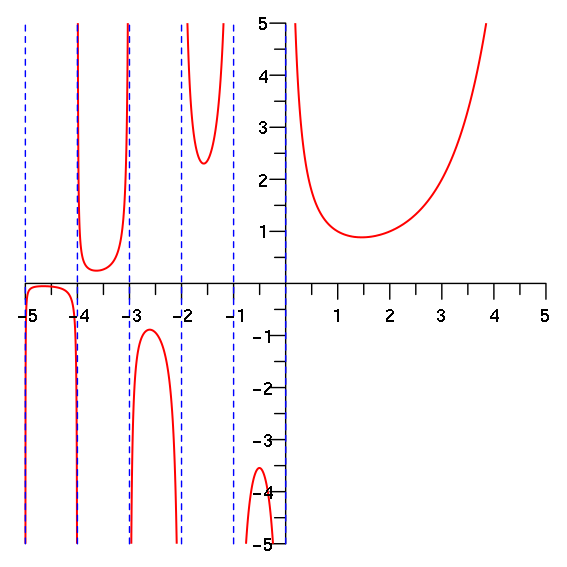
\includegraphics[scale=0.5]{img/2014-01-30/Gammafunktion}
\caption{Quelle: http://commons.wikimedia.org/wiki/File:Gammafunktion.svg}
%TODO: Wer eine Idee hat, wie man das mit tikz machen könnte, ich bin für Vorschläge offen. :)
\end{figure}

\subsection*{Bemerkung}
$\Gamma$ ist eine der wichtigsten Funktionen der Analysis, tritt oft in Normierungskonst. auf.

\phantomsection
\addcontentsline{toc}{section}{Stirlingsche Formel}
\section*{Stirlingsche Formel (Bemerkung zum Wachstum von $n!$)}
$n! \sim \sqrt{2 \pi n} \cdot \left(\frac{n}{e}a\right)^n$\nl
Dabei schreibt man für zwei Folgen $(a_n), (b_n) \subseteq \R$:\\
$a_n \sim b_n :\Lra \lim_{n \to \infty} \frac{a_n}{b_n} = 1$ (asymptotische Gleichheit)\nl
Hier: $\lim_{n \to \infty} \frac{n!}{\sqrt{2 \pi n} \cdot \left(\frac{n}{e}\right)^n} = 1$

\section{Integralkriterium}\label{14.20}
Sei $f: [1,\infty) \to \R$ monoton fallend, $f \ge 0$.\\
$a_n := \sum_{k=1}^n f(k) - \int_1^{n-1} f(x) dx$ ($n \in \N$)\nl
\begin{tikzpicture}
\draw[->] (-0.5,0)--(6,0);
\draw[->] (0,-0.5)--(0,2);
\draw[color=red,pattern=custom north west lines,hatchcolor=red] (0.5,0) -- (0.5,2) -- (1,2) -- (1,0) -- cycle;
\draw[color=red,pattern=custom north west lines,hatchcolor=red] (1,0) -- (1,1) -- (1.5,1) -- (1.5,0) -- cycle;
\draw[color=red,pattern=custom north west lines,hatchcolor=red] (2.5,0) -- (2.5,0.4) -- (3,0.4) -- (3,0) -- cycle;
\draw[color=red,pattern=custom north west lines,hatchcolor=red] (4.5,0) -- (4.5,0.22222222) -- (5,0.22222222) -- (5,0) -- cycle;
\draw[color=green,pattern=custom north west lines,hatchcolor=green] (0.5,2) -- plot [domain=0.5:1] (\x, {1/\x}) -- (1,2) -- cycle;
\draw[color=green,pattern=custom north west lines,hatchcolor=green] (1,1) -- plot [domain=1:1.5] (\x, {1/\x}) -- (1.5,1) -- cycle;
\draw[color=green,pattern=custom north west lines,hatchcolor=green] (2.5,0.4) -- plot [domain=2.5:3] (\x, {1/\x}) -- (3,0.4) -- cycle;
\draw[color=green,pattern=custom north west lines,hatchcolor=green] (4.5,0.22222222) -- plot [domain=4.5:5] (\x, {1/\x}) -- (5,0.22222222) -- cycle;
\draw[color=blue,domain=0.5:5] plot (\x, {1/\x});
\draw (0.5,0) node[below] {$1$} (1,0) node[below] {$2$} (1.5,0) node[below] {$3$} (2,0) node[below] {$\ldots$} (2.5,0) node[below] {\footnotesize $k$} (3,0) node[below] {\footnotesize $k+1$} (3.75,0) node[below] {$\ldots$} (4.5,0) node[below] {\footnotesize $n$} (5,0) node[below] {\footnotesize $n+1$};
\end{tikzpicture}\\
\emph{\footnotesize Der grüne Bereich entspricht $a_n$, der rote dem Integral und beide zusammen der Summe in obiger Gleichung}\nl
$\Ra \lim_{n \to \infty} a_n =: a$ existiert, und $0 \le a \le f(1)$\\
Ferner gilt: $\sum_{k=1}^\infty f(k)$ konvergiert $\Lra \int_1^\infty f(x) dx$ konvergiert
\subsection*{Beweis}
$f$ ist monoton fallend, $f \ge 0$.\nl
$(a_n)$ ist monoton wachsend und beschränkt mit $0 \le a_n \le f(1) \forall n$\\
$\Ra \lim_{n \to \infty} a_n = a$ existiert und $0 \le a \le f(1)$. Rest klar. \qed

\subsection*{Beispiel}
\en{
\item $f(x) = \frac{1}{x^s}, s>1$\\
$\int_1^\infty \frac{dx}{x^s}$ existiert $\Ra \sum_{n=1}^\infty \frac{1}{n^s}$ konvergiert\nl
\underline{Beachte}: $s \le 1 \Ra \sum_{n=1}^\infty \frac{1}{n^s}$ divergiert, da $\frac{1}{n^s} \ge \frac{1}{n}$ (harm. Reihe)\\
\^{=} $\int_1^\infty \frac{dx}{x^s}$ div. für $s<1$
\item $f(x) = \frac{1}{x} \Ra \lim_{n \to \infty} (\sum_{k=1}^n \frac{1}{k} - \ln(n+1)) =:  \gamma \in [0,1]$ existiert \emph{($\gamma$ ist die \href{https://de.wikipedia.org/wiki/Euler-Mascheroni-Konstante}{\underline{Euler-Mascheroni-Konstante}})}\\
d.h. $\sum_{k=1}^n \frac{1}{k} \sim \ln(n+1)$ für $n \to \infty$
}

\chapter{Taylorreihen}\label{P15}
\phantomsection
\addcontentsline{toc}{section}{Taylorpolynome}
\section*{Taylorpolynome}
Lineare Approximation einer differenzierbaren Funktion:\\
Sei $f: I \to \R$ differenzierbar in $a \in I$ und $I$ ein offenes Intervall.\nl
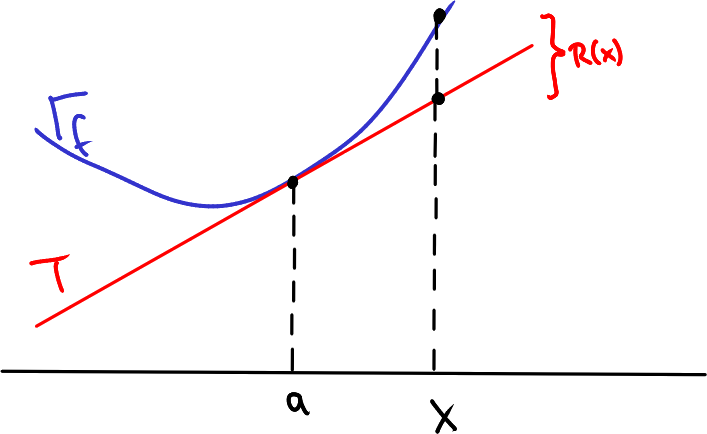
\includegraphics[scale=0.5]{img/2014-01-30/1}\nl %TODO: Vielleicht noch abtikzen?
Tangente an $\Gamma_f$ im Punkt $\underline{(a,f(a))}: T(x) = f(a)+f'(a)(x-a)$\nl
Wie gut ist diese Approximation in der Nähe von $a$?\\
Fehler: $R(x) = f(x)-T(x)$; $R(a) = 0$\\
$x \neq a \Ra \frac{R(x)}{x-a} = \underbrace{\frac{f(x)-f(a)}{x-a}}_{\to f'(a) \text{ für } x \to a} - f'(a) \Ra \lim_{x \to a} \frac{R(x)}{x-a} = 0$\nl
Das heißt, $R(x)$ geht für $x \to a$ deutlich schneller gegen $0$ als $x-a$.

\subsection*{Ziel}
Noch bessere Approximation durch Polynome höheren Grades, falls $f$ genug oft differenzierbar ist in $a$.\nl
Sei $f: I \to \R$ $n$-mal differenzierbar in $a \in I$, $I \subseteq R$ ein offenes Intervall.\\
Gesucht: Polynom $T$, grad $T \le n$, mit $T(a)=f(a)$, $T'(a)=f'(a)$, $T''(a)=f''(a)$, $\ldots$, $T^{(n)}(a) = f^{(n)}(a)$ (*)

\subsection*{Ansatz}
$T(x) = \sum_{k=0}^n c_k (x-a)^k$\\
$\Ra T(a) = c_0$, $T'(a)=c_1$, $T''(a)=2c_2$, $\ldots$, $T^{(n)}(a) = n! \cdot c_n$\\
$\Ra \exists!$ Polynom $T$ vom Grad $\le n$ mit (*), nämlich:
$$T_n f(x; a) = \sum_{k=0}^n \frac{f^{(n)}(a)}{k!} (x-a)^k$$
das \underline{Taylorpolynom} $n$-ter Ordnung an $f$ im Punkt $a$.\nl
$T_n f(x; a) = f(a) + f'(a) \cdot (x-a) + \frac{f''(a)}{2} \cdot (x-a)^2 + \ldots + \frac{f^{(n)}(a)}{n!} (x-a)^n$\nl
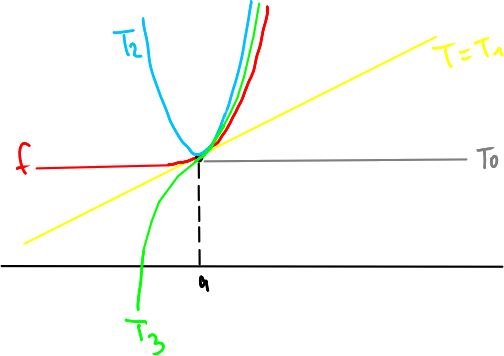
\includegraphics[scale=0.5]{img/2014-01-30/2}\nl %TODO: Vielleicht noch abtikzen?
$T_0 f$ hat den selben Wert wie $f$ in $a$\\
$T_1 f$ hat den selben Wert und die selbe Steigung\\
$T_2 f$ hat den selben Wert, die selbe Steigung und die selbe Krümmung\\
etc.

\subsection*{Beispiel}
$f(x) = \sqrt{1+x}$, $x \in (-1,1) \in I$ (bel. oft differenzierbar auf $I$)\nl
Taylorpolynom zweiter Ordnung von $f$ in $a=0$:\\
$f(0)=1$, $f'(x) = \frac{1}{2} (1+x)^{-\frac{1}{2}}$, $f'(0)=\frac{1}{2}$, $f''(x)=-\frac{1}{4} (1+x)^{-\frac{3}{2}}$, $f''(0) = -\frac{1}{4}$\\
$\Ra T_2 f(x;0) = 1 + \frac{1}{2} x - \frac{1}{8} x^2$

\subsection*{Beobachtung}
Approximationsgüte von $T_n f(x; a)$ nahe $a$?\\
Erwartung: Wird umso besser, je größer $n$ ist.

\subsection*{Restglied}
\fbox{$R_{n+1}(x) := f(x)-T_n f(x; a)$}

\newpage

\section{Satz: Integralformel für das Restglied}\label{15.1}
Sei $f \in C^{n+1} (I)$, $(n \in \N_0)$, $a \in I$ ($C^{n+1}(I)$ ist $n$-mal stetig differenzierbar auf $I$)\\
$\Ra$ \fbox{$R_{n+1}(x) = \frac{1}{n!} \int_a^x (x-t)^n f^{(n+1)}(t) dt$} $\forall x \in I$ (offenes Intervall)

\subsection*{Beweis mit Induktion nach $n$}
\items{
\item[$n=0$:] $R_1(x) = f(x)-f(a) \underset{\text{HDI}}{=} \int_a^x f'(t) dt$ \ok
\item[$n-1 \to n$:] $f(x)-T_{n-1} f(x; a) = R_n(x) \underset{\text{IV}}{=} \frac{1}{(n-1)!} \int_a^x (x-t)^{n-1} f^{(n)}(t) dt$\\
$\underset{\text{part. Int.}}{=} \underbrace{-\frac{(x-t)^n}{n!} f^{(n)} \arrowvert_a^x}_{=\frac{f^(n)(a)}{n!}(x-a)^n} + \frac{1}{n!} \int_a^x (x-t)^n f^{(n+1)}(t) dt$\nl
diesen Term nach links $\Ra$ Behauptung für $n$ \qed
}\newpage %V28
% Kopfzeile beim Kapitelanfang:
\fancypagestyle{plain}{
%Kopfzeile links bzw. innen
\fancyhead[L]{\Large Vorlesung 29 (03.02.2013)}
%Kopfzeile rechts bzw. außen
\fancyhead[R]{}}
%Kopfzeile links bzw. innen
\fancyhead[L]{\Large Vorlesung 29 (03.02.2014)}
%Kopfzeile rechts bzw. außen
\fancyhead[R]{}
% **************************************************
\section{Korollar}\label{15.2}
$f \in C^{n+1}(I)$ mit $f^{(n+1)} \equiv 0$ auf $I$\\
$\Ra f$ ist Polynom vom Grad $\le n$, nämlich $f(x)=T_n f(x; a)$

\section{Satz: Lagrange-Form des Restglieds}\label{15.3}
Sei $f \in C^{n+1}(I)$, $a \in I \Ra \forall x \in I \exists \xi_x$ zwischen $a$ und $x$:
$$R_{n+1}(x) = \frac{f^{(n+1)}(\xi_x)}{(n+1)!} (x-a)^{n+1}$$
Spezialfall $n=0$: $R_1(x)=f(x)-f(a)=f'(\xi_x) \cdot (x-a)$ (MWS der Differentialrechnung, \ref{11.12})

\subsection*{Beweis}
$R_{n+1}(x) = \frac{1}{n!} \int_a^x \underbrace{(x-t)^n}_{p(t)} f^{(n+1)}(t) dt$ hat einheitliches Vorzeichen zwischen $a$ und $x$\\
($x$ ist einzige Nullstelle)\nl
MWS der Integralrechnung (\ref{14.8}) $\Ra R_{n+1}(x) = \frac{1}{n!} f^{(n+1)}(\xi_x) \cdot \underbrace{\int_a^x (x-t)^n dt}_{\frac{1}{n+1}(x-a)^{n+1}}$ ($\xi_x$: geeignete Zwischenstelle zwischen $a$ und $x$)

\subsection*{Anwendung}
Wichtige Anwendung der Lagrange-Form: Abschätzung von $|R_{n+1}(x)|$

\section{Beispiel}\label{15.4}
Gesucht: Näherung für $\sqrt{x}$, $x=1+\delta$, $\delta > 0$ klein\\
Bekannt: $\sqrt{1}=1$\nl
$f(x) := \sqrt{x}$, Taylorentwicklung um $a=1$\\
$n$-te Näherung: $\sqrt{x} = T_n f(x; 1) + R_{n+1}(x)$\\
$f'(x) = \frac{1}{2} \cdot \frac{1}{\sqrt{x}}$, $f''(x) = -\frac{1}{4} \cdot \frac{1}{x^{\frac{3}{2}}}$, $f''(x) = \frac{3}{8} \cdot \frac{1}{x^{\frac{5}{2}}}$, $\ldots$\nl
$|R_n(x)| \underset{\text{Lagrange}}{\le} \frac{|x-1|^n}{n!} \max_{[1,x]} |f^{(n)}| \underset{x>1}{=} \frac{\delta^n}{n!} \cdot |f^{(n)}(1)|$\nl
$n=0$: $\sqrt{x} = f(1)+R_1(x) = 1+R_1(x)$, $|R_1(x)| \le \frac{\delta}{2}$\\
$n=1$: $\sqrt{x} = 1+f'(1) \cdot \delta + R_2(x) = 1+\frac{\delta}{2} + R_2(x)$, $|R_2(x)| \le \frac{\delta^2}{2} \cdot \frac{1}{4} = \frac{\delta^2}{8}$\\
$n=2$: $\sqrt{x} = \underbrace{1+\frac{\delta}{2}-\frac{1}{8} \delta^2}_{T_2 f(x; 1)} + R_3(x)$, $|R_3(x) \le \frac{\delta^3}{16}$

\newpage

\section*{Qualitative Betrachtung}
\underline{Vorbemerkung}: Landau-Symbol "`$o$"'\nl
Seien $f,g: D \to \R$ Funktionen, $a \in \R$\\
Man schreibt: $f(x)=o(g(x))$ für $x \to a$, falls $\lim_{x \to a} \frac{f(x)}{g(x)} = 0$\\
(Analog für $x \to \pm \infty$, falls $D$ nach oben/unten unbeschränkt)

\subsection*{Beispiel}
$|x|^{\frac{3}{2}} = o(x)$ für $x \to 0$; $|x|^{\frac{3}{2}} = o(x^2)$ für $x \to \infty$

\section{Qualitative Taylorformel}\label{15.5}
Sei $f \in C^n(I)$ (nicht notwendig $C^{n+1}$), $a \in I$\\
$\Ra$ \fbox{$f(x) = T_n f(x; a) + o((x-a)^n)$} für $x \to a$

\subsection*{Beweis}
$r(x) := \frac{f(x)-T_n f(x)}{(x-a)^n}$\\
Zu zeigen: $\lim_{x \to a} r(x) = 0$\\
$T_n f(x) = T_{n-1} f(x) + \frac{f^{(n)}(a)}{n!} \cdot (x-a)^n$\\
$r(x) = \underbrace{\frac{f(x) - T_{n-1} f(x)}{(x-a)^n}}_{\text{Lagr.}=\frac{1}{n!} f^{(n)}(\xi)} - \frac{f^{(n)}(a)}{n!} = \frac{1}{n!}(f^{(n)}(\xi) - f^{(n)}(a))$\\
$x \to a \Ra \xi \to a \underset{f^{(n)} \text{ stetig}}{\Ra} f^{(n)}(\xi) \to f^{(n)}(a) \Ra$ Behauptung \qed


\subsection*{Beispiel}
$f(x)=(1+x)^s$ mit $s \in \R, x > -1$\nl
$a := 0$\\
$f(0)=1$; $f'(x) = s(1+x)^{s-1}$; $f'(0) = s \Ra (1+x)^s = 1+sx+o(x)$ für $x \to 0$\\
Das heißt: $\lim_{x \to 0} \frac{(1+x)^s-1-x}{x} = 0$\nl
$s = \frac{1}{2}: \sqrt{1+x} = 1+\frac{1}{2}x+o(x)$ ($x \to 0$)

\section{Definition: Taylorreihen}\label{15.6}
$C^\infty(I) := \{f: I \to \R, f \text{ beliebig oft differenzierbar auf } I\}$\nl
Sei $f \in C^\infty(I)$ \underline{Taylorreihe} von $f$ um $a \in I$.
$$T f(x;a) = \sum_{n=0}^\infty \frac{f^{(n)}(a)}{n!} (x-a)^n$$
Dies ist eine Potenzreihe um $a$ (Entwicklungspunkt)

\newpage

\subsection*{Fakten}
\enk{
\item $T f(x; a)$ konvergiert für festes $x \Lra \lim_{n \to \infty} T_n f(x; a)$ existiert
\item Falls $T f(x; a)$ konvergiert, muss \underline{nicht notwendig} $T f(x; a)=f(x)$ sein!\\
Das heißt, es kann sein, dass $f \in C^\infty(I)$ im Punkt $a \in I$ nicht durch seine Taylorreihe dargestellt wird.
}

\subsection*{Beispiele}
$$f(x) = \left\{\begin{array}{l l} e^{-\frac{1}{x}}, & x > 0 \\ 0, & x \le 0 \end{array}\right.$$
\begin{tikzpicture}
\draw[->] (-3,0)--(3,0);
\draw[->] (0,-0.5)--(0,1.5);
\draw[color=blue,domain=0.1:3] plot (\x, {exp(-1/\x)});
\draw[color=blue,domain=-3:0.1] plot (\x, {0});
\end{tikzpicture}\nl
Es gilt: $f \in C^\infty(\R)$ (kritisch nur $x=0$) mit $f^{(n)}(0)=0 \forall n \in \N_0$\\
$\Ra Tf(x;0) = \sum_{n=0}^\infty \frac{f^{(n)}(0)}{n!} x^n = 0 \forall x \in \R$\nl
Daher: $Tf(x;0) \neq f(x) \forall x>0$!\nl
Aber es gilt:

\section{Satz}\label{15.7}
Sei $f$ eine Funktion mit Potenzreihendarstellung $f(x)=\sum_{n=0}^\infty c_n(x-a)^n$ ($a, c_n \in \R$)\nl
Der Konvergenzradius sei $R > 0 \Ra c_n = \frac{1}{n!} f^{(n)}(a) \forall n \in \N_0$\\
Also: $f(x) = Tf(x;a) \forall x \in (a-R,a+R)$\nl
Man sagt: $f$ besitzt auf $(a-R,a+R)$ eine Taylorentwicklung um $a$ (Beachte: Taylorentwicklung = Potenzreihenentwicklung)

\subsection*{Beweis}
Satz \ref{13.14} $\Ra f \in C^\infty((a-R,a+R))$ und darf gliedweise differenziert werden\nl
$f^{(n)}(x) = \sum_{k=0}^\infty c_k \frac{d^n}{dx^n}(x-a)^k = \sum_{k=n}^\infty c_k \cdot k(k-1) \cdot \ldots \cdot (k-n+1) \cdot (x-a)^{k-n}$\\
$\Ra f^{(n)}(a) \underset{(k=n)}{=} c_n \cdot n!$ \qed\newpage %V29
% Kopfzeile beim Kapitelanfang:
\fancypagestyle{plain}{
%Kopfzeile links bzw. innen
\fancyhead[L]{\Large Vorlesung 30 (06.02.2013)}
%Kopfzeile rechts bzw. außen
\fancyhead[R]{}}
%Kopfzeile links bzw. innen
\fancyhead[L]{\Large Vorlesung 30 (06.02.2014)}
%Kopfzeile rechts bzw. außen
\fancyhead[R]{}
% **************************************************
\section*{Das Newton-Verfahren}\label{Newton-Verfahren}
Zur Berechnung von Nullstellen einer Funktion $f: D \to \R, D \subseteq \R$\nl
Voraussetzung: $f$ ist differenzierbar auf $D$\\
Sei $\xi$ eine Nullstelle von $f$, das heißt: $f(\xi)=0$. Sei $x_0$ eine erste Näherung für $\xi$.\nl
\begin{tikzpicture}
\draw[->] (-3,0)--(3,0);
\draw[color=blue,domain=-2.5:2.5] plot (\x, {(0.15*(\x+2.5)^2)-1.5}) (0.662278,0) node {$\bullet$} node[above] {$\xi$};
\draw[color=red,domain=0:2.5] plot (\x, {(1.35*\x)-1.1625}) (0.861111111,0) node {$\bullet$} node[below] {$x_1$};
\draw[dashed] (2,1.5375) node {$\bullet$} node[right] {$(x_0, f(x_0))$} --(2,0) node[below] {$x_0$};
\end{tikzpicture}

\subsection*{Idee}
Die Nullstelle $x_1$ von $T$ ist bessere Näherung für $\xi$ als $x_0$.\nl
Tangente in $(x_0, f(x_0))$: $T(x)=f(x_0)+f'(x_0)(x-x_0)$\\
$T(x)=0 \Lra x=x_0-\frac{f(x_0)}{f'(x_0)}$, sofern $f'(x_0) \neq 0$\nl
Sei $f'(x_0) \neq 0$. Neue Näherung: $x_1:=x_0-\frac{f(x_0)}{f'(x_0)}$\\
Sei $f'(x_1) \neq 0$. Neue Näherung: $x_2:=x_1-\frac{f(x_1)}{f'(x_1)}$\\
usw.\nl
\begin{tikzpicture}
\draw[->] (-3,0)--(3,0);
\draw[color=blue,domain=-2.5:2.5] plot (\x, {(0.15*(\x+2.5)^2)-1.5}) (0.662278,0) node {$\bullet$} node[above] {$\xi$};
\draw[color=red,domain=-2.5:2.5] plot (\x, {(0.45*\x)-0.7125});
\draw[dashed] (-1,-1.1625) node {$\bullet$} --(-1,0) node{$\bullet$} node[above] {$x_0$};
\draw[color=cyan,domain=0:2.5] plot (\x, {(1.224999*\x)-0.93854});
\draw[color=cyan,dashed] (1.58333,1.001037583335) node {$\bullet$} --(1.58333,0) node {$\bullet$} node[below] {$x_1$};
\draw[color=green] (0.291665,-0.581250666665) node {$\bullet$} node[below] {$x_2$};
\end{tikzpicture}

\newpage

\phantomsection
\addcontentsline{toc}{section}{Definition: Newton-Iteration}
\section*{Definition: Newton-Iteration}
$x_{n+1}=x_n-\frac{f(x_n)}{f'(x_n)}$, sofern $f'(x_n) \neq 0, n \in \N_0$

\subsection*{Beispiel}
Sei $a>0$.\\
Gesucht: $\sqrt{a}$ (Näherung dafür)\nl
$f(x)=x^2-a, f'(x)=2x$\\
$x_{n+1}=x_n-\frac{x_n^2-a}{2x_n} = \frac{1}{2} \cdot \left(x_N + \frac{a}{x_n}\right)$ (auch bekannt als Babylonisches Wurzelziehen, \ref{5.11})

\subsection*{Achtung}
Das Newton-Verfahren kann divergieren, die Konvergenz ist abhängig vom Verhalten von $f$ in der Nähe von $\xi$.

\section{Satz}\label{16.1}
Sei $f: [a,b] \to \R$ eine $C^2$-Funktion (d.h.: zwei Mal stetig differenzierbar auf $[a,b]$) mit:
\en{
\item $f$ hat in $[a,b]$ eine Nullstelle: $\xi$
\item $f'(x) \neq 0 \forall x \in [a,b]$
\item $f''(x) \ge 0 \vee f''(x) \forall x \in [a,b]$
\item Die Iterationen $x_1$ zu $x_0=a$ und $x_0=b$ liegen in $[a,b]$
}
Dann gilt:
\enk{
\item $\xi$ ist einzige Nullstelle von $f$ auf $[a,b]$ (direkt aus (1) und (2))
\item Bei beliebigen $x_0 \in [a,b]$ gilt:\\
$x_n \in [a,b] \forall n, (x_n)$ monoton ab $n=1$, und $\lim_{n \to \infty} x_n = \xi$
\item \underline{Fehlerabschätzung}: $m := \min_{x \in [a,b]} |f'(x)| > 0, M: \max_{x \in [a,b]} |f''(x)|$\\
$\Ra |x_n-\xi| \le \frac{M}{2m} \cdot |x_n-x_{n-1}|^2$\\
(Hat man $x_1,\ldots,x_n$ berechnet, so kann man $|x_n-\xi|$ abschätzen)
}

\newpage

\subsection*{Beweis}
Betrachte Fall $f' > 0 \wedge f'' \ge 0$ (weitere drei Fälle analog)\nl
$g(x) := x - \frac{f(x)}{f'(x)}$ ($\blacksquare$), $g' = 1-\frac{(f')^2-f f''}{(f')^2} = f \cdot \underbrace{\frac{f''}{(f')^2}}_{>0}$\nl
$f$ s.m.w., $f(\xi)=0$\\
$\Ra g'(x) = \left\{\begin{array}{l l l} \le 0 & \text{auf} & [a,\xi] \\ \ge 0 & \text{auf} & [\xi,b]\end{array}\right.$\nl
\begin{tikzpicture}
\draw (-2,0) node {$|$} node[below] {$a$} --(2,0) node {$|$} node[below] {$b$};
\draw[color=blue,domain=-2:2] plot (\x, {(0.25*abs(\x^2))+1.5});
\draw[dashed] (-2,1.5) node[left] {$\xi$} --(0,1.5) --(0,0) node[below] {$\xi$};
\end{tikzpicture}\nl
$\Ra g$ hat absolutes Minimum in $\xi$, $g(\xi)=\xi$; (4) $\Ra g(a), g(b) \in [a,b]$\\
$\Ra \xi \le g(x) \le b \forall x \in [a,b]$ (*)\\
$f \ge 0$ auf $[\xi,b] \Ra g(x) \le x$ auf $[\xi,b]$ (**)\nl
Betrachte nun $(x_n)$: $x_{n+1}=g(x_n)$\nl
\underline{Zu 2.}: $x_0 \in [a,b] \underset{\text{(*)}}{\Ra} x_1 = g(x_0) \in [\xi,b]$\\
Ist $x_n \in [\xi,b]$ gezeigt für $n \in \N \Ra \xi \le \underbrace{g(x_n)}_{x_{n+1}} \underset{\text{(**)}}{\le} x_n \le b \Ra x_{n+1} \in [\xi,b]$\nl
Also: Induktion $\Ra (x_n) \subseteq [\xi,b]$ und monoton fallend ab $n=1$\\
$\Ra x_n \to \hat{\xi} \in [\xi,b]$\nl
$x_0 \in [a,b]$ beliebig, $x_{n+1}=g(x_n), n \in \N_0$\\
$(x_n)_{n \ge 1} \subseteq [\xi,b]$ monoton fallend $\Ra \hat{\xi} := \lim_{n \to \infty} x_n \in [\xi,b]$ existiert\\
$\hat{\xi} = \lim_{n \to \infty} x_{n+1} = \lim_{n \to \infty} g(x_n) \underset{g \text{ stetig}}{=} g(\lim_{n \to \infty} x_n) = g(\hat{\xi})$\\
($\blacksquare$) $\Ra f(\hat{\xi})=0 \underset{\text{Teil 1.}}{\Ra} \hat{\xi}=\xi$\nl
\underline{Zur Fehlerabschätzung}: $x_n \neq \xi \Ra \left|\frac{f(x_n)-\overbrace{f(\xi)}^{=0}}{x_n-\xi}\right| \underset{\text{MWS}}{=} |f'(\mu)| \ge m > 0$ ($\mu$ zwischen $\xi, x_n$)\\
$\Ra |x_n-\xi| \le \frac{|f(x_n)|}{m} \forall n$\nl
Abschätzung von $f(x_n)$: Taylorentwicklung von $f$ um $x_{n-1}$:\\
Lagrange (\ref{15.3}) $\Ra f(x_n) = \underbrace{f(x_{n-1})+f'(x_{n-1}) \cdot (x_n-x_{n-1})}_{=0} + \frac{1}{2} f''(\overline{\mu}) \cdot (x_n-x_{n-1})^2$ ($\overline{\mu}$ zwischen $x_{n-1}, x_n$)\\
$\Ra |f(x_n)| = \frac{1}{2} |f''(\overline{\mu})| \cdot |x_n-x_{n-1}|^2 \le \frac{M}{2} \cdot |x_n-x_{n-1}|^2$\\
$\Ra |x_n-\xi| \le \frac{M}{2m} \cdot |x_n-x_{n-1}|^2$ \qed

\newpage

\subsection*{Beispiel}
$f(x)=x-e^{-x} \overset{!}{=} 0$\\
$f(0)=-1<0, f(1)=1-\frac{1}{e} > 0$\nl
$[a,b]=[0,1]$ wählbar, denn:
\en{
\item erfüllt nach ZWS \ok
\item $f'(x)=1+e^{-x} > 0$ \ok
\item $f''(x)=-e^{-x} < 0$ \ok
\item $x_0=0 \Ra x_1 = \frac{1}{2} [0,1], x_0=1 \Ra x_1=\frac{2}{1+e} \in [0,1]$ \ok
}
$m = 1+\frac{1}{e}, M=1$\nl
Konkretes Beispiel: Startwert $x_0 := \frac{1}{2}$ (1. Iteration zu $0$)\\
$x_1 = 0,566311\ldots$\\
$x_2 = 0,567143\ldots$\\
$|x_2-\xi| \le \frac{M}{2m} |x_2-x_1|^2 < 0,5 \cdot 10^{-6}$\newpage %V30
% Kopfzeile beim Kapitelanfang:
\fancypagestyle{plain}{
%Kopfzeile links bzw. innen
\fancyhead[L]{\Large Informationen zur Klausur}
%Kopfzeile rechts bzw. außen
\fancyhead[R]{}}
%Kopfzeile links bzw. innen
\fancyhead[L]{\Large Informationen zur Klausur}
%Kopfzeile rechts bzw. außen
\fancyhead[R]{}
% **************************************************

\phantomsection
\addcontentsline{toc}{chapter}{Infos zur 1. Klausur WS 2013/14}
\chapter*{Infos zur 1. Klausur WS 2013/14}
\section*{Grundsätzliches zur Klausur}
\items{
%\item 20. Februar 2014, 13:30-15:30 Uhr in der Sporthalle SP2 (\href{http://www.uni-paderborn.de/fileadmin/uni-homepage/images/lageplan-03.13.jpg?dur=357}{\emph{\underline{Lageplan}}})
%\item Es wird wahrscheinlich \textbf{6 Aufgaben} geben
\item Keine Aufgabe ist optional, alle sind zu bearbeiten und gehen vollständig in die Zielnote mit ein
\item Ein beidseitig handbeschriebener DIN-A4 Spicker ist als Hilfsmittel zugelassen
\item Weitere Hilfsmittel (u.a. Taschenrechner) sind nicht zugelassen!
}

\section*{Aufgaben der ersten Klausur}
\emph{Folgendes ist aus meinem Gedächtnisprotokoll der ersten Klausur.\\
Dieses, andere sowie Klausuren der Vorjahre können in der Fachschaft (E1.311) eingesehen werden.}\nl

\noindent \textbf{Aufgabe 1: Rekursive Folgen}\newline
Gegeben: eine rekursive Definition für $(a_n)$
\begin{enumerate}[label=(\alph*)]
\item Beweis mit vollständiger Induktion, dass sich $a_n$ zwischen zwei Werten aufhält
\item Zeigen Sie Monotonie der Folge
\item Prüfen Sie, ob die Folge konvergiert, und wenn, dann berechnen Sie den Grenzwert
\end{enumerate}

\bigskip \hrule \bigskip

\noindent \textbf{Aufgabe 2: Komplexe Zahlen}
\begin{enumerate}[label=(\alph*)]
\item Wandeln Sie zwei gegebene, komplexe Zahlen um in das Format $x+yi$
\item Berechnen Sie von einer gegebenen, komplexen Zahl $z$ (nicht im Format $x+yi$) den Betrag $|z|$
\end{enumerate}

\bigskip \hrule \bigskip

\noindent \textbf{Aufgabe 3: Differentialrechnung}\newline
Gegeben: eine Funktion $f$
\begin{enumerate}[label=(\alph*)]
\item Skizzieren Sie den Graphen der Funktion
\item Wo ist die Funktion differenzierbar? Berechnen Sie dort die Ableitung
\end{enumerate}

\bigskip \hrule \bigskip

\noindent \textbf{Aufgabe 4: Konvergenzradius}\newline
Gegeben: Potenzreihe
\begin{enumerate}[label=(\alph*)]
\item Berechnen Sie den Konvergenzradius dieser Reihe
\item Wo konvergiert diese Reihe?
\end{enumerate}

\newpage

\noindent \textbf{Aufgabe 5: Kurvendiskussion, Trigonometrie}\newline
Zeigen Sie, dass eine gegeben Funktion $f$ genau eine Nullstelle in einem gegebenen, halboffenen Intervall hat

\bigskip \hrule \bigskip

\noindent \textbf{Aufgabe 6: Kurvendiskussion, Logarithmus}
\begin{enumerate}[label=(\alph*)]
\item Berechnen Sie für $x \to \infty$ den Grenzwert von einem gegebenen Term mit Logarithmus Naturalis
\item Untersuchen Sie die Funktion diesen Terms auf lokale und globale Extrema
\end{enumerate}

\bigskip \hrule \bigskip

\noindent \textbf{Aufgabe 7: Integralrechnung}
\begin{enumerate}[label=(\alph*)]
\item Berechnen Sie den Wert eines gegebenen Integrals
\item Zeigen/widerlegen Sie, dass ein gegebenes Integral konvergiert
\end{enumerate}

%\items{
%\item Folgen, Grenzwerte, rekursive Folgen (wie in Zwischenklausur)
%\item Komplexe Zahlen (z.B. Einheitswurzel)
%\item Potenzreihen, Konvergenzradien
%\item Reihen, Reihenkonvergenz, Leibniz-Kriterium
%\item Stetigkeit
%\item Ableitungen
%\item Hauptsatz der Integral- und Differentialrechnung
%\item Zwischen-, Mittelwertsatz
%\item Integralrechnung, uneigentliche Integrale, partielle Integrale, Substitution
%\item Taylorpolynome
%}\newpage
\end{document}
